%% LyX 2.3.3 created this file.  For more info, see http://www.lyx.org/.
%% Do not edit unless you really know what you are doing.
\documentclass[12pt,english]{article}
\usepackage[osf]{mathpazo}
\renewcommand{\sfdefault}{lmss}
\renewcommand{\ttdefault}{lmtt}
\usepackage[T1]{fontenc}
\usepackage[latin9]{inputenc}
\usepackage[paperwidth=30cm,paperheight=35cm]{geometry}
\geometry{verbose,tmargin=2cm,bmargin=2cm}
\setlength{\parindent}{0bp}
\usepackage{mathrsfs}
\usepackage{amsmath}
\usepackage{amssymb}

\makeatletter
\@ifundefined{date}{}{\date{}}
%%%%%%%%%%%%%%%%%%%%%%%%%%%%%% User specified LaTeX commands.
\usepackage{tikz}
\usetikzlibrary{matrix,arrows,decorations.pathmorphing}
\usetikzlibrary{shapes.geometric}
\usepackage{tikz-cd}
\usepackage{amsthm}
\usepackage{xparse,etoolbox}

\theoremstyle{plain}
\newtheorem{theorem}{Theorem}[section]
\newtheorem{lemma}[theorem]{Lemma}
\newtheorem{prop}{Proposition}[section]
\newtheorem*{cor}{Corollary}
\theoremstyle{definition}
\newtheorem{defn}{Definition}[section]
\newtheorem{ex}{Exercise} 
\newtheorem{example}{Example}[section]
\theoremstyle{remark}
\newtheorem*{rem}{Remark}
\newtheorem*{note}{Note}
\newtheorem{case}{Case}
\usepackage{graphicx}
\usepackage{amssymb}
\usepackage{tikz-cd}
\usetikzlibrary{calc,arrows,decorations.pathreplacing}
\tikzset{mydot/.style={circle,fill,inner sep=1.5pt},
commutative diagrams/.cd,
  arrow style=tikz,
  diagrams={>=latex},
}

\usepackage{babel}
\usepackage{hyperref}
\hypersetup{
    colorlinks,
    citecolor=blue,
    filecolor=blue,
    linkcolor=blue,
    urlcolor=blue
}
\usepackage{pgfplots}
\usetikzlibrary{decorations.markings}
\pgfplotsset{compat=1.9}


\newcommand{\blocktheorem}[1]{%
  \csletcs{old#1}{#1}% Store \begin
  \csletcs{endold#1}{end#1}% Store \end
  \RenewDocumentEnvironment{#1}{o}
    {\par\addvspace{1.5ex}
     \noindent\begin{minipage}{\textwidth}
     \IfNoValueTF{##1}
       {\csuse{old#1}}
       {\csuse{old#1}[##1]}}
    {\csuse{endold#1}
     \end{minipage}
     \par\addvspace{1.5ex}}
}

\raggedbottom

\blocktheorem{theorem}% Make theo into a block
\blocktheorem{defn}% Make defi into a block
\blocktheorem{lemma}% Make lem into a block
\blocktheorem{rem}% Make rem into a block
\blocktheorem{cor}% Make col into a block
\blocktheorem{prop}% Make prop into a block


\makeatletter
\newcommand*{\@old@slash}{}\let\@old@slash\slash
\def\slash{\relax\ifmmode\delimiter"502F30E\mathopen{}\else\@old@slash\fi}
\makeatother

\def\backslash{\delimiter"526E30F\mathopen{}}



\usepackage[bottom]{footmisc}

\makeatother

\usepackage{babel}
\begin{document}
\title{Linear Analysis}

\maketitle
\tableofcontents{}

\pagebreak{}

\part{Class Notes}

\section{Inner-Product Spaces}

\begin{defn}\label{defn} Let $V$ be a vector space over $\mathbb{C}$.
A map $\langle\cdot,\cdot\rangle\colon V\times V\to\mathbb{C}$ is
called an \textbf{inner-product on $V$ }if it satisfies the following
properties:
\begin{enumerate}
\item Linearity in the first argument: $\langle x,z\rangle+\langle y,z\rangle=\langle x+y,z\rangle$
and $\langle\lambda x,y\rangle=\lambda\langle x,y\rangle$ for all
$x,y,z\in V$ and $\lambda\in\mathbb{C}$.
\item Conjugate symmetric: $\langle x,y\rangle=\overline{\langle y,x\rangle}$
for all $x,y\in V$.
\item Positive definite: $\langle x,x\rangle>0$ for all nonzero $x\in V$.
\end{enumerate}
A vector space equipped with an inner-product is called an \textbf{inner-product
space}. We often write $\mathcal{V}$ to denote an inner-product space.
\end{defn}

\begin{prop}\label{prop} Let $\mathcal{V}$ be an inner-product space.
Then
\begin{enumerate}
\item $\langle x,y+z\rangle=\langle x,y\rangle+\langle x,z\rangle$ for
all $x,y,z\in\mathcal{V}$;
\item $\langle x,\lambda y\rangle=\overline{\lambda}\langle x,y\rangle$
for all $x,y\in\mathcal{V}$ and $\lambda\in\mathbb{C}$
\item $\langle x,0\rangle=0=\langle0,x\rangle$ for all $x\in\mathcal{V}$;
\item Let $x,y\in\mathcal{V}$. If $\langle x,z\rangle=\langle y,z\rangle$
for all $z\in\mathcal{V}$, then $x=y$. 
\end{enumerate}
\end{prop}

\begin{proof}\hfill
\begin{enumerate}
\item Let $x,y,z\in\mathcal{V}$. Then
\begin{align*}
\langle x,y+z\rangle & =\overline{\langle y+z,x\rangle}\\
 & =\overline{\langle y,x\rangle+\langle z,x\rangle}\\
 & =\overline{\langle y,x\rangle}+\overline{\langle z,x\rangle}\\
 & =\langle x,y\rangle+\langle x,z\rangle.
\end{align*}
\item Let $x,y\in\mathcal{V}$ and $\lambda\in\mathbb{C}$. Then 
\begin{align*}
\langle x,\lambda y\rangle & =\overline{\langle\lambda y,x\rangle}\\
 & =\overline{\lambda\langle y,x\rangle}\\
 & =\overline{\lambda}\overline{\langle y,x\rangle}\\
 & =\overline{\lambda}\langle x,y\rangle.
\end{align*}
\item Let $x\in\mathcal{V}$. Then 
\begin{align*}
\langle x,0\rangle & =\langle x,0+0\rangle\\
 & =\langle x,0\rangle+\langle x,0\rangle
\end{align*}
implies $\langle x,0\rangle=0$. A similar argument gives $\langle0,x\rangle=0$. 
\item Assuming $\langle x,z\rangle=\langle y,z\rangle$ for all $z\in\mathcal{V}$,
then we have $\langle x-y,z\rangle=0$ for all $z\in\mathcal{V}$.
In particular, setting $z=x-y$, we have $\langle x-y,x-y\rangle=0$.
Since the inner-product is positive definite, we must have $x-y=0$,
and hence $x=y$. 
\end{enumerate}
\end{proof}

\subsection{Examples of Inner-Product Spaces}

If we are given a complex vector space $V$, then we can \textbf{give
$V$ the structure of an inner-product space }by equipping $V$ with
an inner-product 
\[
\langle\cdot,\cdot\rangle\colon V\times V\to\mathbb{C}.
\]
In the following examples, we give many familiar complex vector spaces
the structure of an inner-product space.

\subsubsection{Giving $\mathbb{C}^{n}$ the structure of an inner-product space}

\begin{prop}\label{prop} Let $\langle\cdot,\cdot\rangle\colon\mathbb{C}^{n}\times\mathbb{C}^{n}\to\mathbb{C}$
be given by
\[
\langle x,y\rangle=\langle(x_{1},\dots,x_{n}),(y_{1},\dots,y_{n})\rangle=\sum_{i=1}^{n}x_{i}\overline{y}_{i}.
\]
for all $x,y\in\mathbb{C}^{n}$. Then the pair $(\mathbb{C}^{n},\langle\cdot,\cdot\rangle)$
forms an inner-product space. \end{prop}

\begin{proof}\label{proof} For linearity in the first argument follows
from linearity, let $x,y,z\in\mathbb{C}^{n}$. Then
\begin{align*}
\langle x+y,z\rangle & =\sum_{i=1}^{n}(x_{i}+y_{i})\overline{z}_{i}\\
 & =\sum_{i=1}^{n}x_{i}\overline{z}_{i}+\sum_{i=1}^{n}y_{i}\overline{z}_{i}\\
 & =\langle x,z\rangle+\langle y,z\rangle.
\end{align*}

For conjugate symmetry of $\langle\cdot,\cdot\rangle$, let $x,y\in\mathbb{C}^{n}$.
Then
\begin{align*}
\langle x,y\rangle & =\sum_{i=1}^{n}x_{i}\overline{y}_{i}\\
 & =\sum_{i=1}^{n}\overline{\overline{x_{i}\overline{y}_{i}}}\\
 & =\sum_{i=1}^{n}\overline{y_{i}\overline{x}_{i}}\\
 & =\overline{\langle y,x\rangle}.
\end{align*}

For positive-definiteness of $\langle\cdot,\cdot\rangle$, let $x\in\mathbb{C}^{n}$.
Then
\begin{align*}
\langle x,x\rangle & =\sum_{i=1}^{n}x_{i}\overline{x}_{i}\\
 & =\sum_{i=1}^{n}|x_{i}|^{2}.
\end{align*}
is a sum of its components absolute squared. This implies positive-definiteness.
\end{proof}

\subsubsection{Giving $\text{M}_{m\times n}(\mathbb{C})$ the structure of an inner-product
space}

Since $\text{M}_{m\times n}(\mathbb{C})\cong\mathbb{C}^{mn}$, we
can give $\text{M}_{m\times n}(\mathbb{C})$ the structure of an inner-product
space by equipping it with the inner-product described in the previous
example. In more detail, let $E_{ij}$ be the standard matrix in $\text{M}_{m\times n}(\mathbb{C})$
whose entry in the $(i,j)$-th component is $1$ and whose entry everywhere
else is $0$, let $e_{k}$ be the standard basis vector in $\mathbb{C}^{mn}$
whose entry in the $k$-th compenent is $1$ and whose entry everywhere
else is $0$, and let $\varphi\colon\text{M}_{m\times n}(\mathbb{C})\to\mathbb{C}^{mn}$
be the isomorphism such that 
\[
\varphi(E_{ij})=e_{n(i-1)+j}
\]
for all $E_{ij}\in\text{M}_{m\times n}(K)$ where $1\leq i\leq m$
and $1\leq j\leq n$. So under $\varphi$, we have
\[
A:=\begin{pmatrix}a_{11} & \cdots & a_{1n}\\
\vdots & \ddots & \vdots\\
a_{m1} & \cdots & a_{mn}
\end{pmatrix}\mapsto\begin{pmatrix}a_{11}\\
\vdots\\
a_{1n}\\
\vdots\\
a_{m1}\\
\vdots\\
a_{mn}
\end{pmatrix}:=a
\]

Using this isomorphism, we give $\text{M}_{m\times n}(\mathbb{C})$
the structure of an inner-product space by defining 
\[
\langle\cdot,\cdot\rangle\colon\text{M}_{m\times n}(\mathbb{C})\times\text{M}_{m\times n}(\mathbb{C})\to\mathbb{C}
\]
by the formula
\[
\langle A,B\rangle:=\text{Tr}(AB^{*})=\sum_{j=1}^{n}\sum_{i=1}^{m}a_{ij}\overline{b}_{ij}=\langle a,b\rangle
\]
where 
\[
A=\begin{pmatrix}a_{11} & \cdots & a_{1n}\\
\vdots & \ddots & \vdots\\
a_{m1} & \cdots & a_{mn}
\end{pmatrix}\quad,B=\begin{pmatrix}b_{11} & \cdots & b_{1n}\\
\vdots & \ddots & \vdots\\
b_{m1} & \cdots & b_{mn}
\end{pmatrix},\quad\text{and}\quad B^{*}=\begin{pmatrix}\overline{b}_{11} & \cdots & \overline{b}_{m1}\\
\vdots & \ddots & \vdots\\
\overline{b}_{1n} & \cdots & \overline{b}_{nm}
\end{pmatrix}.
\]


\subsubsection{Giving $\ell^{2}(\mathbb{N})$ the structure of an inner-product
space}

\begin{lemma}\label{lemmainequality} Let $a$ and $b$ be nonnegative
real numbers. Then we have
\begin{equation}
ab\leq\frac{1}{2}(a^{2}+b^{2})\label{eq:inequality}
\end{equation}
with equality if and only if $a=b$. \end{lemma}

\begin{prop}\label{prop} Let $\ell^{2}(\mathbb{N})$ be the set of
all sequence $(x_{n})$ in $\mathbb{C}$ such that 
\[
\sum_{n=1}^{\infty}|x_{n}|^{2}<\infty
\]
and let $\langle\cdot,\cdot\rangle\colon\ell^{2}(\mathbb{N})\times\ell^{2}(\mathbb{N})\to\mathbb{C}$
be given by
\[
\langle(x_{n}),(y_{n})\rangle=\sum_{n=1}^{\infty}x_{n}\overline{y}_{n}.
\]
for all $(x_{n}),(y_{n})\in\ell^{2}(\mathbb{N})$. Then the pair $(\ell^{2}(\mathbb{N}),\langle\cdot,\cdot\rangle)$
forms an inner-product space. \end{prop}

\begin{proof}\label{proof} We first need to show that $\ell^{2}(\mathbb{N})$
is indeed a vector space. In fact, we will show that $\ell^{2}(\mathbb{N})$
is a subspace of $\mathbb{C}^{N}$, the set of all sequences in $\mathbb{C}$.
Let $(x_{n}),(y_{n})\in\ell^{2}(\mathbb{N})$ and $\lambda\in\mathbb{C}$.
Then Lemma~(\ref{lemmainequality}) implies
\begin{align*}
\sum_{n=1}^{\infty}|\lambda x_{n}+y_{n}|^{2} & \leq\sum_{n=1}^{\infty}|\lambda x_{n}|^{2}+\sum_{n=1}^{\infty}|y_{n}|^{2}+\sum_{n=1}^{\infty}2|\lambda x_{n}||y_{n}|\\
 & \leq\lambda^{2}\sum_{n=1}^{\infty}|x_{n}|^{2}+\sum_{n=1}^{\infty}|y_{n}|^{2}+\lambda^{2}\sum_{n=1}^{\infty}|x_{n}|^{2}+|y_{n}|^{2}\\
 & <\infty.
\end{align*}
Therefore $(\lambda x_{n}+y_{n})\in\ell^{2}(\mathbb{N})$, which implies
$\ell^{2}(\mathbb{N})$ is a subspace of $\mathbb{C}^{\mathbb{N}}$. 

~~~Next, let us show that the inner product converges, and hence
is defined everywhere. Let $(x_{n}),(y_{n})\in\ell^{2}(\mathbb{N})$.
Then it follows from Lemma~(\ref{lemmainequality}) that
\begin{align*}
\sum_{n=1}^{\infty}|x_{n}\overline{y}_{n}| & =\sum_{n=1}^{\infty}|x_{n}||y_{n}|\\
 & \leq\sum_{n=1}^{\infty}\frac{|x_{n}|^{2}+|y_{n}|^{2}}{2}\\
 & =\frac{1}{2}\sum_{n=1}^{\infty}|x_{n}|^{2}+\frac{1}{2}\sum_{n=1}^{\infty}|y_{n}|^{2}\\
 & <\infty.
\end{align*}
Therefore $\sum_{n=1}^{\infty}x_{n}\overline{y}_{n}$ is absolutely
convergent, which implies it is convergent. (We can't use Cauchy-Schwarz
here since we haven't yet shown that $\langle\cdot,\cdot\rangle$
is in fact an inner-product).

~~~Finally, let us shows that $\langle\cdot,\cdot\rangle$ is an
inner-product. Linearity in the first argument follows from distrubitivity
of multiplication and linearity of taking infinite sums. For conjugate
symmetry, let $(x_{n}),(y_{n})\in\ell^{2}(\mathbb{N})$. Then
\begin{align*}
\langle(x_{n}),(y_{n})\rangle & =\sum_{n=1}^{\infty}x_{n}\overline{y}_{n}\\
 & =\lim_{N\to\infty}\sum_{n=1}^{N}x_{n}\overline{y}_{n}\\
 & =\overline{\overline{\lim_{N\to\infty}\sum_{n=1}^{N}x_{n}\overline{y}_{n}}}\\
 & =\overline{\lim_{N\to\infty}\sum_{n=1}^{N}\overline{x_{n}\overline{y}_{n}}}\\
 & =\overline{\lim_{N\to\infty}\sum_{n=1}^{N}y_{n}\overline{x}_{n}}\\
 & =\overline{\sum_{n=1}^{\infty}y_{n}\overline{x}_{n}}\\
 & =\overline{\langle(y_{n}),(x_{n})\rangle},
\end{align*}
where we were allowed to bring the conjugate inside the limit since
the conjugate function is continuous on $\mathbb{C}$. For positive-definiteness,
let $(x_{n})\in\ell^{2}(\mathbb{N})$. Then 
\begin{align*}
\langle(x_{n}),(x_{n})\rangle & =\sum_{n=1}^{\infty}x_{n}\overline{x}_{n}\\
 & =\sum_{n=1}^{\infty}|x_{n}|^{2}\\
 & \geq0.
\end{align*}
If $\sum_{n=1}^{\infty}|x_{n}|^{2}=0$, then clearly we must have
$x_{n}=0$ for all $n$. \end{proof}

\subsubsection{Giving $C[a,b]$ the structure of an inner-product space}

\begin{prop}\label{prop} Let $C[a,b]$ be the space of all continuous
functions defined on the closed interval $[a,b]$ and let $\langle\cdot,\cdot\rangle\colon C[a,b]\times C[a,b]\to\mathbb{C}$
be given by
\[
\langle f,g\rangle=\int_{a}^{b}f(x)\overline{g(x)}dx
\]
for all $f,g\in C[a,b]$. Then the pair $(C[a,b],\langle\cdot,\cdot\rangle)$
forms an inner-product space. \end{prop}

\begin{proof} Exercise.\end{proof}

\subsection{Norm Induced by Inner-Product }

\begin{defn}\label{defnnormofinner} The \textbf{norm }of $x\in\mathcal{V}$,
denoted $\|x\|$, is defined by
\[
\|x\|=\sqrt{\langle x,x\rangle}.
\]

\end{defn}

\begin{lemma}\label{pythagoreantheoremlemma} (Pythagorean Theorem)
Let $x$ and $y$ be nonzero vectors in $\mathcal{V}$ such that $\langle x,y\rangle=0$
(we call such vectors \textbf{orthogonal }to one another). Then 
\[
\|x+y\|^{2}=\|x\|^{2}+\|y\|^{2}.
\]
\end{lemma}

\begin{proof} We have
\begin{align*}
\|x+y\|^{2} & =\langle x+y,x+y\rangle\\
 & =\langle x,x\rangle+\langle x,y\rangle+\langle y,x\rangle+\langle y,y\rangle\\
 & =\langle x,x\rangle+\langle y,y\rangle\\
 & =\|x\|^{2}+\|y\|^{2}
\end{align*}

\end{proof}

\subsubsection{Properties of Norm}

\begin{prop}\label{propinnerprodnorm} If $x,y\in\mathcal{V}$ and
$\lambda\in\mathbb{C}$, then 
\begin{enumerate}
\item Positive-Definiteness: $\|x\|\geq0$ with equality if and only if
$x=0$; 
\item Absolutely Homogeneous: $\|\lambda x\|=|\lambda|\|x\|$;
\item Cauchy-Schwarz: $|\langle x,y\rangle|\leq\|x\|\|y\|$ with equality
if and only if $x$ and $y$ are linearly dependent.
\item Subadditivity: $\|x+y\|\leq\|x\|+\|y\|$
\end{enumerate}
\end{prop}

\begin{proof} \hfill
\begin{enumerate}
\item This follows from positive-definiteness of $\langle\cdot,\cdot\rangle$. 
\item We have 
\begin{align*}
\|\lambda x\| & =\sqrt{\langle\lambda x,\lambda x\rangle}\\
 & =\sqrt{\lambda\overline{\lambda}\langle x,x\rangle}\\
 & =\sqrt{|\lambda|^{2}\langle x,x\rangle}\\
 & =|\lambda|\sqrt{\langle x,x\rangle}\\
 & =|\lambda|\|x\|.
\end{align*}
\item We may assume that both $x$ and $y$ are nonzero, since it is trivial
in this case. Let 
\[
z=x-\text{pr}_{y}(x)=x-\frac{\langle x,y\rangle}{\langle y,y\rangle}y.
\]
Then by linearity of the inner product in the first argument, one
has 
\begin{align*}
\langle z,y\rangle & =\left\langle x-\frac{\langle x,y\rangle}{\langle y,y\rangle}y,y\right\rangle \\
 & =\langle x,y\rangle-\frac{\langle x,y\rangle}{\langle y,y\rangle}\langle y,y\rangle\\
 & =0.
\end{align*}
Therefore $z$ is a vector orthogonal to the vector $y$. We can thus
apply the Pythagorean theorem to 
\[
x=\frac{\langle x,y\rangle}{\langle y,y\rangle}y+z
\]
which gives 
\begin{align*}
\|x\|^{2} & =\left|\frac{\langle x,y\rangle}{\langle y,y\rangle}\right|^{2}\|y\|^{2}+\|z\|^{2}\\
 & =\frac{|\langle x,y\rangle|}{(\|y\|^{2})^{2}}^{2}\|y\|^{2}+\|z\|^{2}\\
 & =\frac{|\langle x,y\rangle|}{\|y\|^{2}}^{2}+\|z\|^{2}\\
 & \geq\frac{|\langle x,y\rangle|^{2}}{\|y\|^{2}},
\end{align*}
and after multiplication by $\|y\|^{2}$ and taking square root, we
get the Cauchy-Schwarz inequality. Moreover, if the relation $\geq$
in the above expression is actually an equality, then $\|z\|^{2}=0$
and hence $z=0$; the definition of $z$ then establishes a relation
of linear dependence between $x$ and $y$. On the other hand, if
$x$ and $y$ are linearly dependent, then there exists $\lambda\in\mathbb{C}$
such that $x=\lambda y$. Then 
\begin{align*}
|\langle x,y\rangle| & =|\langle\lambda y,y\rangle|\\
 & =|\lambda||\langle y,y\rangle|\\
 & =|\lambda|\|y\|^{2}\\
 & =\|\lambda y\|\|y\|\\
 & =\|x\|\|y\|.
\end{align*}
\item By the Cauchy-Schwarz inequality, we have
\begin{align*}
\|x+y\|^{2} & =\langle x+y,x+y\rangle\\
 & =\langle x,x\rangle+\langle x,y\rangle+\langle y,x\rangle+\langle y,y\rangle\\
 & =\|x\|^{2}+2\text{Re}(\langle x,y\rangle)+\|y\|^{2}\\
 & \leq\|x\|^{2}+2|\langle x,y\rangle|+\|y\|^{2}\\
 & \leq\|x\|^{2}+2\|x\|\|y\|+\|y\|^{2}\\
 & =(\|x\|+\|y\|)^{2}
\end{align*}
now we take square roots on both sides to get the desired result. 
\end{enumerate}
\end{proof}

\begin{prop}\label{propparallelogram} (Parallelogram Identity) Let
$x,y\in\mathcal{V}$. Then
\begin{equation}
\|x-y\|^{2}+\|x+y\|^{2}=2\|x\|^{2}+2\|y\|^{2}\label{eq:parallelogram}
\end{equation}
\end{prop}

\begin{proof} We have 
\begin{align*}
\|x+y\|^{2} & =\langle x+y,x+y\rangle\\
 & =\langle x,x\rangle+\langle x,y\rangle+\langle y,x\rangle+\langle y,y\rangle\\
 & =\|x\|^{2}+2\text{Re}(\langle x,y\rangle)+\|y\|^{2}.
\end{align*}
and
\begin{align*}
\|x-y\|^{2} & =\langle x-y,x-y\rangle\\
 & =\langle x,x\rangle+\langle x,-y\rangle+\langle-y,x\rangle+\langle-y,-y\rangle\\
 & =\|x\|^{2}-2\text{Re}(\langle x,y\rangle)+\|y\|^{2}.
\end{align*}
Adding these together gives us our desired result. \end{proof}

\begin{prop}\label{prop} (Polarization Identity) Let $x,y\in\mathcal{V}$.
Then
\[
4\langle x,y\rangle=\|x+y\|^{2}+i\|x+iy\|^{2}-\|x-y\|^{2}-i\|x-iy\|^{2}
\]
\end{prop}

\begin{proof} We have
\begin{align*}
\|x+y\|^{2} & =\langle x+y,x+y\rangle\\
 & =\langle x,x\rangle+\langle x,y\rangle+\langle y,x\rangle+\langle y,y\rangle,
\end{align*}
and
\begin{align*}
i\|x+iy\|^{2} & =i\langle x+iy,x+iy\rangle\\
 & =i\langle x,x\rangle+i\langle x,iy\rangle+i\langle iy,x\rangle+i\langle iy,iy\rangle\\
 & =i\langle x,x\rangle+\langle x,y\rangle-\langle y,x\rangle+i\langle y,y\rangle,
\end{align*}
and
\begin{align*}
-\|x-y\|^{2} & =-\langle x-y,x-y\rangle\\
 & =-\langle x,x\rangle-\langle x,-y\rangle-\langle-y,x\rangle-\langle-y,-y\rangle\\
 & =-\langle x,x\rangle+\langle x,y\rangle+\langle y,x\rangle-\langle y,y\rangle,
\end{align*}
and
\begin{align*}
-i\|x-iy\|^{2} & =-i\langle x-iy,x-iy\rangle\\
 & =-i\langle x,x\rangle-i\langle x,-iy\rangle-i\langle-iy,x\rangle-i\langle-iy,-iy\rangle\\
 & =-i\langle x,x\rangle+\langle x,y\rangle-\langle y,x\rangle-i\langle y,y\rangle.
\end{align*}
Adding these together gives us our desired result. \end{proof}

\subsubsection{Normed Vector Spaces}

\begin{defn}\label{normedvectorspace} Let $V$ be a $\mathbb{C}$-vector
space. A \textbf{norm }on $V$ is a nonnegative-valued scalar function
$\|\cdot\|\colon V\to[0,\infty)$ such that for all $\lambda\in\mathbb{C}$
and $x,y\in V$, we have 
\begin{enumerate}
\item (Subadditivity) $\|x+y\|\leq\|x\|+\|x\|$,
\item (Absolutely Homogeneous) $\|\lambda x\|=|\lambda|\|x\|$,
\item (Positive-Definite) $\|x\|=0$ if and only if $x=0$.
\end{enumerate}
We call the pair $(V,\|\cdot\|)$ a \textbf{normed vector space}.
\end{defn}

Proposition~(\ref{propinnerprodnorm}) implies $\mathcal{V}$ is a
normed vector space. This justifies our choice of the word ``norm''
in Definition~(\ref{defnnormofinner}). Proposition~(\ref{propinnerprodnorm})
also tells us that $\mathcal{V}$ satisfies an extra property which
is not satisfied by other normed vector spaces, namely the Cauchy-Schwarz
inequality. In fact, it turns out that inner-product spaces are just
normed vector spaces which satisfy the parallelogram law.

\subsubsection{Metric Induced By Norm}

\begin{defn}\label{defn} A \textbf{metric }on a set $X$ is a function
$d\colon X\times X\to\mathbb{R}$ which satisfies the following three
properties:
\begin{enumerate}
\item (Identity of Indiscernibles) $d(x,y)=0$ if and only if $x=y$ for
all $x,y\in X$,
\item (Symmetric) $d(x,y)=d(y,x)$ for all $x,y\in X$,
\item (Triangle Inequality) $d(x,z)\leq d(x,y)+d(y,z)$ for all $x,y,z\in X$.
\end{enumerate}
A set $X$ together with a choice of a metric $d$ is called a \textbf{metric
space }and is denoted $(X,d)$, or just denoted $X$ if the metric
is understood from context. \end{defn}

\begin{rem}\label{rem} Given the three axioms above, we also have
positive-definiteness: $d(x,y)\geq0$ with equality if and only if
$x=y$ for all $x,y\in X$. Indeed,
\begin{align*}
0 & =d(x,x)\\
 & \leq d(x,y)+d(y,x)\\
 & =d(x,y)+d(x,y)\\
 & =2d(x,y).
\end{align*}
This implies $d(x,y)\geq0$. \end{rem}

\begin{prop}\label{prop} Let $(V,\|\cdot\|)$ be a normed vector
space. Define $d\colon V\times V\to\mathbb{R}$ by $d(x,y)=\|x-y\|$
for all $(x,y)\in V\times V$. Then $(V,d)$ is a metric space. \end{prop}

\begin{proof} Let us first check that $d$ satisfies the identity
of indiscernibles property. Since $\|\cdot\|$ is positive-definite,
$d(x,y)=0$ implies $\|x-y\|=0$ which implies $x=y$. On the other
hand, suppose $x=y$. Then since $\|\cdot\|$ is absolutely homogeneous,
we have $\|0\|=|0|\|0\|=0$, and so $d(x,y)=\|0\|=0$. 

~~~Next we check that $d$ is symmetric. For all $(x,y)\in V\times V$,
we have
\begin{align*}
d(x,y) & =\|x-y\|\\
 & =\|-(y-x)\|\\
 & =|-1|\|y-x\|\\
 & =\|y-x\|\\
 & =d(y,x).
\end{align*}
~~~Finally, triangle inequality for $d$ follows from subadditivity
of $\|\cdot\|$. Indeed, for all $x,y,z\in V$, we have
\begin{align*}
d(x,y)+d(y,z) & =\|x-y\|+\|y-z\|\\
 & \geq\|x-z\|\\
 & =d(x,z).
\end{align*}

\end{proof}

The distance between points $x,y\in\mathcal{V}$ is measured using
the metric induced by the norm:
\[
d(x,y):=\|x-y\|.
\]

\begin{defn}\label{defn} A sequence $(x_{n})$ in $\mathcal{V}$
is said to converge to a point $x\in\mathcal{V}$ if for all $\varepsilon>0$
there exists $N\in\mathbb{N}$ such that 
\[
n\geq N\text{ implies }\|x_{n}-x\|<\varepsilon.
\]
In this case we write $x_{n}\to x$ as $n\to\infty$ or more simply
$x_{n}\to x$. We also write
\[
\lim_{n\to\infty}x_{n}=x.
\]
 

\end{defn}

\begin{prop}\label{prop} Let $(x_{n})$ and $(y_{n})$ be two sequences
in $\mathcal{V}$ and let $(\lambda_{n})$ be a sequence in $\mathbb{C}$.
Then the following statements hold:
\begin{enumerate}
\item There exists $M\geq0$ such that $\|x_{n}\|\leq M$ for all $n\in\mathbb{N}$. 
\item If $x_{n}\to x$ and $y_{n}\to y$, then $x_{n}+y_{n}\to x+y$. 
\item If $(\lambda_{n})$ is a sequence in $\mathbb{C}$ and $\lambda_{n}\to\lambda$,
then $\lambda_{n}x_{n}\to\lambda x$. 
\item If $x_{n}\to x$ and $y_{n}\to y$, then $\langle x_{n},y_{n}\rangle\to\langle x,y\rangle$.
In particular, $\|x_{n}\|\to\|x\|$. 
\end{enumerate}
\end{prop}

\begin{proof} \hfill
\begin{enumerate}
\item Choose $N\in\mathbb{N}$ such that $n\geq N$ implies $\|x_{n}-x\|\leq1$.
Now set $M$ to be 
\[
M=\max\{\|x_{1}\|,\dots,\|x_{N-1}\|,\|x\|+1\}
\]
\item Let $\varepsilon>0$. Choose $N\in\mathbb{N}$ such that $n\geq N$
implies $\|x_{n}-x\|<\varepsilon/2$ and $\|y_{n}-y\|<\varepsilon/2$.
Then $n\geq N$ implies 
\begin{align*}
\|x_{n}+y_{n}-(x+y)\| & \leq\|x_{n}-x\|+\|y_{n}-y\|\\
 & <\varepsilon/2+\varepsilon/2\\
 & =\varepsilon.
\end{align*}
\item Since $x_{n}\to x$, there exists $M\geq0$ such that $\|x_{n}\|\leq M$
for all $n\in\mathbb{N}$. Choose such an $M$ and let $\varepsilon>0$.
Choose $N\in\mathbb{N}$ such that $n\geq N$ implies $\|x_{n}-x\|<\varepsilon/2|\lambda|$
and $|\lambda_{n}-\lambda|<\varepsilon/2M$. Then $n\geq N$ implies
\begin{align*}
\|\lambda_{n}x_{n}-\lambda x\| & =\|\lambda_{n}x_{n}-\lambda x_{n}+\lambda x_{n}-\lambda x\|\\
 & \leq\|\lambda_{n}x_{n}-\lambda x_{n}\|+\|\lambda x_{n}-\lambda x\|\\
 & \leq\|(\lambda_{n}-\lambda)x_{n}\|+\|\lambda(x_{n}-x)\|\\
 & =|\lambda_{n}-\lambda|\|x_{n}\|+|\lambda|\|x_{n}-x\|\\
 & \leq|\lambda_{n}-\lambda|M+|\lambda|\|x_{n}-x\|\\
 & <\varepsilon/2+\varepsilon/2\\
 & =\varepsilon.
\end{align*}
\item Since $y_{n}\to y$, there exists $M\geq0$ such that $\|y_{n}\|\leq M$
for all $n\in\mathbb{N}$. Choose such an $M$ and let $\varepsilon>0$.
Choose $N\in\mathbb{N}$ such that $n\geq N$ implies $\|x_{n}-x\|<\varepsilon/2M$
and $\|y_{n}-y\|<\varepsilon/2\|x\|$. Then $n\geq N$ implies
\begin{align*}
|\langle x_{n},y_{n}\rangle-\langle x,y\rangle| & =|\langle x_{n},y_{n}\rangle-\langle x,y_{n}\rangle+\langle x,y_{n}\rangle-\langle x,y\rangle|\\
 & \leq|\langle x_{n},y_{n}\rangle-\langle x,y_{n}\rangle|+|\langle x,y_{n}\rangle-\langle x,y\rangle|\\
 & =|\langle x_{n}-x,y_{n}\rangle|+|\langle x,y_{n}-y\rangle|\\
 & \leq\|x_{n}-x\|\|y_{n}\|+\|x\|\|y_{n}-y\|\\
 & \leq\|x_{n}-x\|M+\|x\|\|y_{n}-y\|\\
 & <\varepsilon/2+\varepsilon/2\\
 & =\varepsilon.
\end{align*}
To see that $\|x_{n}\|\to\|x\|$, we just set $y_{n}=x_{n}$. Then
\begin{align*}
\|x_{n}\| & =\sqrt{\langle x_{n},x_{n}\rangle}\\
 & \to\sqrt{\langle x,x\rangle}\\
 & =\|x\|,
\end{align*}
where we were allowed to take limits inside the square root function
since the square root function is continuous on $\mathbb{R}_{\geq0}$. 
\end{enumerate}
\end{proof}

\begin{defn}\label{defn} Let $\|\cdot\|_{1}$ and $\|\cdot\|_{2}$
be two norms on a vector space $V$. We say $\|\cdot\|_{1}$ is \textbf{stronger
}than $\|\cdot\|_{2}$ (or $\|\cdot\|_{2}$ is \textbf{weaker }than
$\|\cdot\|_{1}$) if there exists a constant $C>0$ such that 
\[
\|x\|_{2}\leq C\|x\|_{1}
\]
for all $x\in V$. \end{defn}

\begin{rem}\label{rem} Observe if a sequence $(x_{n})$ in $V$ converges
to $x$ in the metric spaced induced by the $\|\cdot\|_{1}$ norm,
then it also converges in the metric space induced by the $\|\cdot\|_{2}$
norm. Indeed, let $\varepsilon>0$. Choose $N\in\mathbb{N}$ such
that $n\geq N$ implies $\|x_{n}-x\|_{1}<\varepsilon/C$. Then $n\geq N$
implies
\begin{align*}
\|x_{n}-x\|_{2} & \leq C\|x_{n}-x\|_{1}\\
 & <\varepsilon.
\end{align*}

Thus a sequence $(x_{n})$ converging in the $\|\cdot\|_{1}$ norm
is a \emph{stronger }condition than\emph{ }the sequence $(x_{n})$
converging in the $\|\cdot\|_{2}$ norm. An alternative way of thinking
about this is that the topology induced by the $\|\cdot\|_{1}$ norm
is \emph{finer }than the topology induced by the $\|\cdot\|_{2}$
norm. Indeed, if $B_{r}^{2}(0)$ is the open ball of radius $r$ centered
at $0$ in the $\|\cdot\|_{2}$ norm and $B_{r/C}^{1}(0)$ is the
open ball of radius $r/C$ in the $\|\cdot\|_{1}$ norm, then we have
\[
B_{r}^{2}(0)\subseteq B_{r/C}^{1}(0).
\]
More generally, if $a\in V$, then
\begin{align*}
B_{r}^{2}(a) & =a+B_{r}^{2}(0)\\
 & \subseteq a+B_{r/C}^{1}(0)\\
 & =B_{r/C}^{1}(a).
\end{align*}
This implies the topology induced by $\|\cdot\|_{1}$ is finer than
the topology induced by $\|\cdot\|_{2}$. \end{rem}

\subsection{Closure}

\begin{defn}\label{defn} Let $A\subseteq\mathcal{V}$. A point $x\in\mathcal{V}$
is said to be a \textbf{closure} \textbf{point }of $A$ if every open
neighborhood of $x$ meets $A$. This means that for any $\varepsilon>0$,
we have $B_{\varepsilon}(x)\cap A\neq\emptyset$, where 
\[
B_{\varepsilon}(x):=\{y\in\mathcal{V}\mid\|x-y\|<\varepsilon\}.
\]

The \textbf{closure of $A$ }is the set of all closure points of $A$
and is denoted $\overline{A}$. \end{defn}

\begin{rem}\label{rem} If every open neighborhood of a point $x\in\mathcal{V}$
meets $A$, then we can find a sequence $(x_{n})$ of points in $A$
such that $x_{n}\to x$. Conversely, if $(x_{n})$ is a sequence of
points in $A$ such that $x_{n}\to x$, then every open neighborhood
of $x$ meets $A$. Thus, an equivalent condition for $x$ to be a
closure point of $A$ is that there exists a sequence $(x_{n})$ of
points in $A$ such that $x_{n}\to x$. We will prove this in a moment.
\end{rem} 

\begin{prop}\label{prop} Let $A,B\subseteq\mathcal{V}$. Then
\begin{enumerate}
\item $A\subseteq\overline{A}$;
\item If $A\subseteq B$, then $\overline{A}\subseteq\overline{B}$;
\item $\overline{A\cup B}=\overline{A}\cup\overline{B}$;
\item $\overline{A\cap B}\subseteq\overline{A}\cap\overline{B}$;
\item $\overline{\overline{A}}=\overline{A}$.
\end{enumerate}
\end{prop}

\begin{proof}\label{proof}\hfill
\begin{enumerate}
\item Let $x\in A$. Then every open neighborhood of $x$ meets $A$ since,
in particular, every open neighborhood meets $x\in A$. Therefore
$x\in\overline{A}$.
\item Let $x\in\overline{A}$. Then every open neighborhood of $x$ meets
$B$ since, in particular, each open neighborhood meets $A$. Therefore
$x\in\overline{B}$.
\item First note that $\overline{A\cup B}\supseteq\overline{A}\cup\overline{B}$
follows from 2. For the reverse inclusion, let $x\in\overline{A\cup B}$
and assume for a contradiction that $x\notin\overline{A}\cup\overline{B}$.
Then there exists a open neighborhood $U$ of $x$ such that $U\cap A=\emptyset$
and an open neighborhood $V$ of $x$ such that $V\cap A=\emptyset$.
Choose such open neighborhoods $U$ and $V$ and set $W=U\cap V$.
Then $W$ is a open neighborhood of $x$ such that 
\[
W\cap(A\cup B)=(W\cap A)\cup(W\cap B)=\emptyset,
\]
which contradicts the fact that $x\in\overline{A\cup B}$.
\item This follows from 2. To see why we do not necessarily get the reverse
equality, consider $A=(0,1)$ and $B=(1,2)$ in $\mathbb{R}$. Then
$\overline{A}\cap\overline{B}=\{1\}$ but $\overline{A\cap B}=\overline{\emptyset}=\emptyset$.
\item Exercise.
\end{enumerate}
\end{proof}

\begin{prop}\label{prop} $x\in\overline{A}$ if and only if there
exists a sequence $(x_{n})$ of elements in $A$ such that $x_{n}\to x$.
\end{prop}

\begin{proof}\label{proof} Assume $x\in\overline{A}$. For each $n\in\mathbb{N}$,
choose $x_{n}\in B_{1/n}(x)\cap A$ (this set is nonempty since $x\in\overline{A})$.
Then one readily checks that $x_{n}\to x$.

~~~Conversely, suppose that $(x_{n})$ in $A$ such that $x_{n}\to x$
and assume for a contradiction that $x\notin\overline{A}$. Then there
exists an open neighborhood $B_{\varepsilon}(x)$ of $x$ such that
$B_{\varepsilon}(x)\cap A=\emptyset$. Choose such an open neighborhood
and choose $N\in\mathbb{N}$ such that $1/N<\varepsilon$. Then $n\geq N$
implies 
\[
x_{n}\in B_{1/N}(x)\cap A\subseteq B_{\varepsilon}(x)\cap A,
\]
which is a contradiction. \end{proof}

\begin{defn}\label{defn} A set $A\subseteq\mathcal{V}$ is said to
be a \textbf{closed set }if $A=\overline{A}$. \end{defn}

~~~In finite dimensional inner-product spaces every subspace is
a closed set. However this is no longer true in infinite dimensional
spaces.

\begin{example}\label{example} Let $\ell_{0}(\mathbb{N})$ be the
subset of $\ell^{2}(\mathbb{N})$ consisting of all square summable
sequences $(x_{n})$ with only finitely many nonzero terms. It is
easy to see that $\ell_{0}(\mathbb{N})$ is in fact a subspace of
$\ell^{2}(\mathbb{N})$. However $\ell_{0}(\mathbb{N})$ is not a
\emph{closed }subspace of $\ell^{2}(\mathbb{N})$. Indeed, consider
the sequence of elements in $\ell_{0}(\mathbb{N})$ given by 
\begin{align*}
x^{1} & =(1,0,0,0,\cdots)\\
x^{2} & =(1,1/2,0,0,\cdots)\\
x^{3} & =(1,1/2,1/3,0,\dots)\\
 & \vdots
\end{align*}
Then the sequence $(x^{n})$ of sequences $x^{n}$ converges to the
sequence $(1/n)\notin\ell_{0}(\mathbb{N})$. Therefore $\ell_{0}(\mathbb{N})$
is not closed.

~~~To see why we have $(x^{n})\to(1/n)$, let $\varepsilon>0$.
Choose $N\in\mathbb{N}$ such that $\sum_{k=N}^{\infty}1/k^{2}<\varepsilon$
(there exists such an $N$ since $\sum_{k=0}^{\infty}1/k^{2}<\infty$).
Then for all $n\geq N$, we have 
\[
\|(x^{n})-(1/n)\|\leq\sum_{k=N}^{\infty}\frac{1}{k^{2}}<\varepsilon.
\]

\end{example}

\begin{theorem}\label{theoremclosureofsubspaceissubspace} Let $\mathcal{U}$
be a subspace of $\mathcal{V}$. Then $\overline{\mathcal{U}}$ is
a subspace of $\mathcal{V}$. \end{theorem}

\begin{proof} Let $x,y\in\overline{\mathcal{U}}$ and $\lambda\in\mathbb{C}$.
Let $(x_{n})$ and $(y_{n})$ be two sequences of elements in $\mathcal{U}$
such that $x_{n}\to x$ and $y_{n}\to y$. Then $(\lambda x_{n}+y_{n})$
is a sequence of elements in $\mathcal{U}$ such that $\lambda x_{n}+y_{n}\to\lambda x+y$.
Therefore $\lambda x+y\in\overline{\mathcal{U}}$, which implies $\overline{\mathcal{U}}$
is a subspace of $\mathcal{V}$. \end{proof}

\begin{prop}\label{prop} If $\mathcal{U}$ is a subspace of $\mathcal{V}$,
then the closure $\overline{\mathcal{V}}$ is a closed subspace. \end{prop}

\begin{proof}\label{proof} Clearly $\overline{\mathcal{U}}$ is a
closed set. Therefore it suffices to show that $\overline{\mathcal{U}}$
is a subspace of $\mathcal{V}$. Let $x,y\in\overline{\mathcal{U}}$
and let $\lambda\in\mathbb{C}$. Choose sequence $(x_{n})$ and $(y_{n})$
in $\mathcal{U}$ such that $x_{n}\to x$ and $y_{n}\to y$. Then
since $\lambda x_{n}+y_{n}\in\mathcal{U}$ for each $n\in\mathbb{N}$
and 
\[
\lim_{n\to\infty}(\lambda x_{n}+y_{n})=\lambda x+y,
\]
we have $\lambda x+y\in\overline{\mathcal{U}}$. Therefore $\overline{\mathcal{U}}$
is a subspace of $\mathscr{V}$. \end{proof}

\section{Hilbert Spaces}

Let $\mathcal{V}$ be an inner-product space. A sequence $(x_{n})\in\mathcal{V}$
is said to be a \textbf{Cauchy sequence }if for all $\varepsilon>0$
there exists $N\in\mathbb{N}$ such that 
\[
n,m\geq N\text{ implies }\|x_{n}-x_{m}\|<\varepsilon.
\]
Every convergent sequence in $\mathcal{V}$ is a Cauchy sequence.
Indeed:

\begin{prop}\label{prop} Let $\mathcal{V}$ be an inner-product space
and let $(x_{n})$ be a convergent sequence in $\mathcal{V}$. Then
$(x_{n})$ is a Cauchy sequence. \end{prop}

\begin{proof}\label{proof} Let $x\in\mathcal{V}$ be the limit of
$(x_{n})$ and let $\varepsilon>0$. Choose $N\in\mathbb{N}$ such
that $n\geq N$ implies $\|x_{n}-x\|<\varepsilon/2$. Then $m,n\geq N$
implies 
\begin{align*}
\|x_{n}-x_{m}\| & =\|x_{n}-x+x-x_{m}\|\\
 & \leq\|x_{n}-x\|+\|x-x_{m}\|\\
 & <\varepsilon/2+\varepsilon/2\\
 & =\varepsilon.
\end{align*}
It follows that $(x_{n})$ is Cauchy. \end{proof}

~~~Though every convergent sequence is Cauchy, the converse need
not hold. For instance, in $\mathbb{Q}$, we can construct a sequence
of rational numbers which gets closer and closer to $\pi$. Namely,
such a sequence starts out as
\begin{equation}
(3,3.1,3.14,3.141,\dots).\label{eq:sequenceconvtopi}
\end{equation}
It's easy to see that such a sequence is in fact a Cauchy sequence.
However, by construction, this sequence converges to $\pi$, which
is not a rational number. On the other hand, since $\pi$ is a real
number, the Cauchy sequence (\ref{eq:sequenceconvtopi}) of real numbers
converges to a real number. Is every Cauchy sequence in $\mathbb{R}$
convergent? It turns out that the answer to this is, yes! We give
a special name to inner-product spaces which share this property with
$\mathbb{R}$. 

\begin{defn}\label{defn} Let $\mathcal{V}$ be an inner-product space.
We say $\mathcal{V}$ is a \textbf{Hilbert space }if every Cauchy
sequence in $\mathcal{V}$ converges to a limit in $\mathcal{V}$.
\end{defn}

~~~The most basic examples with Hilbert spaces are $\mathbb{R}$,
$\mathbb{R}^{n}$, and $\mathbb{C}^{n}$ (with their usual inner-product).
We will show later on that $\ell^{2}(\mathbb{N})$ is also a Hilbert
space. Nonexamples of Hilbert spaces include $\mathbb{Q}$ and $C[a,b]$.
Hilbert spaces are usually denoted by $\mathcal{H}$ and $\mathcal{K}$.

\subsection{Distances}

\begin{defn}\label{defndistance} Let $\mathcal{V}$ be an inner-product
space, let $A,B\subseteq\mathcal{V}$, and let $x\in\mathcal{V}$.
We define the \textbf{distance from $x$ to $A$}, denoted $\mathrm{d}(x,A)$,
by
\[
\mathrm{d}(x,A):=\inf\{\|x-a\|\mid a\in A\}.
\]
More generally, we defined the \textbf{distance from $A$ to $B$},
denoted $\mathrm{d}(A,B)$, by
\[
\mathrm{d}(A,B):=\inf\{\|a-b\|\mid a\in A\quad\text{and}\quad b\in B\}.
\]
\end{defn}

\begin{prop}\label{prop} With the notation as in Definition~(\ref{defndistance}),
we have $\mathrm{d}(x,A)=0$ if and only if $x\in\overline{A}$. \end{prop}

\begin{proof} Suppose $\mathrm{d}(x,A)=0$. Then for each $n\in\mathbb{N}$
we can choose $a_{n}\in A$ such that
\[
\mathrm{d}(x,A)\leq\|x-a_{n}\|<\mathrm{d}(x,A)+\frac{1}{n}.
\]
In other words, since $\mathrm{d}(x,A)=0$, we can find a sequence
$(a_{n})$ in $A$ such that
\[
\|x-a_{n}\|<\frac{1}{n}
\]
for all $n\in\mathbb{N}$. This implies $x\in\overline{A}$. 

~~~Conversely, suppose $x\in\overline{A}$. Then we can find a
sequence $(a_{n})$ in $A$ such that
\[
\mathrm{d}(x,A)\leq\|x-a_{n}\|<\frac{1}{n}
\]
for all $n\in\mathbb{N}$. Taking $n\to\infty$ gives us $\mathrm{d}(x,A)=0$.
\end{proof}

\begin{rem}\label{rem} A common technique that we do is we choose
a sequence $(a_{n})$ of elements in $A$ such that
\[
\|x-a_{n}\|<d(x,A)+\frac{1}{n}
\]
for all $n\in\mathbb{N}$. Such a sequence must exist since otherwise
there would exist an $n\in\mathbb{N}$ such that
\[
d(x,A)+\frac{1}{n}\leq\|x-a\|
\]
for all $a\in A$, and this contradicts the fact that $d(x,A)$ is
the infimum. \end{rem}

\subsubsection{Absolute Homogeneity of Distances}

\begin{prop}\label{prop} Let $\mathcal{V}$ be an inner-product space,
let $\mathcal{A}$ be a subspace of $\mathcal{V}$, let $x\in\mathcal{V}$,
and let $\lambda\in\mathbb{C}$. Then 
\[
d(\lambda x,\mathcal{A})=|\lambda|d(x,\mathcal{A}).
\]
\end{prop}

\begin{proof} Choose a sequence $(y_{n})$ of elements in $\mathcal{A}$
such that
\[
\|x-y_{n}\|<d(x,\mathcal{A})+\frac{1}{|\lambda n|}
\]
for all $n\in\mathbb{N}$. Then since $\mathcal{A}$ is a subspace,
we have
\begin{align*}
d(\lambda x,\mathcal{A}) & \leq\|\lambda x-\lambda y_{n}\|\\
 & =|\lambda|\|x-y_{n}\|\\
 & <|\lambda|\left(d(x,\mathcal{A})+\frac{1}{|\lambda n|}\right)\\
 & =|\lambda|d(x,\mathcal{A})+\frac{1}{n}
\end{align*}
for all $n\in\mathbb{N}$. In particular, this implies $d(\lambda x,\mathcal{A})\leq|\lambda|d(x,\mathcal{A})$. 

~~~Conversely, choose a sequence $(z_{n})$ of elements in $\mathcal{A}$
such that
\[
\|\lambda x-z_{n}\|<d(\lambda x,\mathcal{A})+\frac{1}{n}
\]

Then since $\mathcal{A}$ is a subspace, we have
\begin{align*}
|\lambda|d(x,\mathcal{A}) & \leq|\lambda|\|x-z_{n}/|\lambda|\|\\
 & =\|\lambda x-z_{n}\|\\
 & <d(\lambda x,\mathcal{A})+\frac{1}{n}
\end{align*}
for all $n\in\mathbb{N}$. In particular, this implies $|\lambda|d(x,\mathcal{A})\leq d(\lambda x,\mathcal{A})$.
\end{proof}

\subsubsection{Subadditivity of Distances}

\begin{prop}\label{prop} Let $\mathcal{V}$ be an inner-product space,
let $\mathcal{A}$ be a subspace of $\mathcal{V}$, and let $x,y\in\mathcal{V}$.
Then 
\[
d(x+y,\mathcal{A})\leq d(x,\mathcal{A})+d(y,\mathcal{A}).
\]
\end{prop}

\begin{proof} Choose a sequences $(w_{n})$ and $(z_{n})$ of elements
in $\mathcal{A}$ such that 
\[
\|x-w_{n}\|<d(x,\mathcal{A})+\frac{1}{2n}\quad\text{and}\quad\|y-z_{n}\|<d(y,\mathcal{A})+\frac{1}{2n}
\]
for all $n\in\mathbb{N}$. Then since $\mathcal{A}$ is a subspace,
we have
\begin{align*}
d(x+y,\mathcal{A}) & \leq\|(x+y)-(w_{n}+z_{n})\|\\
 & \leq\|x-w_{n}\|+\|y-z_{n}\|\\
 & <d(x,\mathcal{A})+\frac{1}{2n}+d(y,\mathcal{A})+\frac{1}{2n}\\
 & =d(x,\mathcal{A})+d(y,\mathcal{A})+\frac{1}{n}
\end{align*}
for all $n\in\mathbb{N}$. In particular, this implies $d(x+y,\mathcal{A})\leq d(x,\mathcal{A})+d(y,\mathcal{A})$.
\end{proof}

\subsection{Orthogonal Projection}

Let $K$ be a $2$-dimensional subspace in $\mathbb{R}^{3}$. Such
a subspace corresponds to a plane in $\mathbb{R}^{3}$ which passes
through the origin. One of the main tools that we use in this setting
is the concept of projecting onto $K$. For instance, if $K$ corresponds
to the plane $\{z=0\}$ in $\mathbb{R}^{3}$, then the projection
of the vector $(1,2,1)^{\top}$ onto $K$ gives the vector $(1,2,0)^{\top}$.
In fact, $(1,2,0)^{\top}$ is the \emph{closest }vector to $(1,2,1)^{\top}$
which belongs to $K$. In other words, if $(a,b,0)^{\top}\in K$,
then
\begin{align*}
\sqrt{(1-a)^{2}+(2-b)^{2}+1} & =\|(1,2,1)^{\top}-(a,b,0)^{\top}\|\\
 & \geq\|(1,2,1)^{\top}-(1,2,0)^{\top}\|\\
 & =1.
\end{align*}
We wish to generalize these concepts from $\mathbb{R}^{3}$ to an
arbitrary Hilbert space. 

\begin{theorem}\label{theoremorthogonalprojectionexist} Let $\mathcal{H}$
be a Hilbert space and let $\mathcal{K}$ be a closed subspace of
$\mathcal{H}$. Suppose $x\in\mathcal{H}\backslash\mathcal{K}$. Then
there exists a unique $a\in\mathcal{K}$ such that $\mathrm{d}(x,\mathcal{K})=\|x-a\|$.
\end{theorem}

\begin{proof}\label{proof} Choose a sequence $(a_{n})$ of elements
in $\mathcal{K}$ such that
\begin{equation}
\mathrm{d}(x,\mathcal{K})\leq\|x-a_{n}\|<\mathrm{d}(x,\mathcal{K})+1/n.\label{eq:inequalityinf}
\end{equation}
for all $n\in\mathbb{N}$. We claim that $(a_{n})$ is a Cauchy sequence.
The key to showing this is to use the parallelogram identity, which
says 
\begin{equation}
\|y-z\|^{2}+\|y+z\|^{2}=2\|y\|^{2}+2\|z\|^{2}\label{eq:paralleltoprove}
\end{equation}
for all $y,z\in\mathcal{H}$. Setting $y=x-a_{m}$ and $z=x-a_{n}$
in (\ref{eq:paralleltoprove}) and rearranging terms, we have

\begin{align*}
\|a_{m}-a_{n}\|^{2} & =2\|x-a_{m}\|^{2}+2\|x-a_{n}\|^{2}-\|(x-a_{m})+(x-a_{n})\|^{2}\\
 & <2(\mathrm{d}(x,\mathcal{K})+1/m)^{2}+2(\mathrm{d}(x,\mathcal{K})+1/n)^{2}-\|(2(x-(a_{n}-a_{m})/2)\|^{2}\\
 & =4\mathrm{d}(x,\mathcal{K})^{2}+(4/m+4/n)\mathrm{d}(x,\mathcal{K})+2/m^{2}+2/n^{2}-4\|(x-(a_{n}-a_{m})/2\|^{2}\\
 & \leq4\mathrm{d}(x,\mathcal{K})^{2}+(4/m+4/n)\mathrm{d}(x,\mathcal{K})+2/m^{2}+2/n^{2}-4\mathrm{d}(x,\mathcal{K})^{2}\\
 & =(4/n+4/m)\mathrm{d}(x,\mathcal{K})+2/n^{2}+2/m^{2}.
\end{align*}
Thus if $\varepsilon>0$, then we choose $N\in\mathbb{N}$ such that
$n,m\geq N$ implies
\[
(4/n+4/m)\mathrm{d}(x,\mathcal{K})+2/n^{2}+2/m^{2}<\varepsilon^{2}.
\]
which implies $\|a_{m}-a_{n}\|<\varepsilon$. Therefore the sequence
$(a_{n})$ is a Cauchy sequence, and since we are in a Hilbert space,
$(a_{n})$ must be convergent, say $a_{n}\to a$, with $a\in\mathcal{K}$
since $\mathcal{K}$ is closed. Then taking the limit of (\ref{eq:inequalityinf})
as $n\to\infty$ gives us $\mathrm{d}(x,\mathcal{K})=\|x-a\|$.

~~~To see uniqueness of $a$, let $b$ be another point in $\mathcal{K}$
such that $\|x-b\|=\mathrm{d}(x,\mathcal{K})$. We again use the parallelogram
identity. We have
\begin{align*}
\|b-a\|^{2} & =\|(x-a)-(x-b)\|^{2}\\
 & =2\|x-a\|^{2}+2\|x-b\|^{2}-\|(x-a)+(x-b)\|^{2}\\
 & =4\mathrm{d}(x,\mathcal{K})^{2}-\|2x-(a+b)\|^{2}\\
 & =4\mathrm{d}(x,\mathcal{K})^{2}-4\|x-(a+b)/2\|^{2}\\
 & \leq0,
\end{align*}
which implies $a=b$. \end{proof}

\begin{theorem}\label{theoremuniqueorthproj} Let $\mathcal{H}$ be
a Hilbert space, let $\mathcal{K}$ be a closed subspace of $\mathcal{H}$,
and let $x\in\mathcal{H}$. Then $\mathrm{P}_{\mathcal{K}}x$ is the
unique point in $\mathcal{K}$ such that
\[
\langle x-\mathrm{P}_{\mathcal{K}}x,y\rangle=0
\]
for all $y\in\mathcal{K}$. \end{theorem}

\begin{proof}\label{proof} Let $y\in\mathcal{K}$. Define a function
$f\colon\mathbb{R}\to\mathbb{R}$ by
\[
f(t)=\|x-\mathrm{P}_{\mathcal{K}}x+ty\|^{2}
\]
for all $t\in\mathbb{R}$. Then $f(0)=\mathrm{d}(x,\mathcal{K})^{2}$
and $f(t)>\mathrm{d}(x,\mathcal{K})^{2}$ for all $t\neq0$ (note
we have a \emph{strict }inequality here by uniqueness of $\mathrm{P}_{\mathcal{K}}x$).
For each $t\in\mathbb{R}$, we have
\begin{align*}
f(t) & =\|x-\mathrm{P}_{\mathcal{K}}x+ty\|^{2}\\
 & =\langle x-\mathrm{P}_{\mathcal{K}}x+ty,x-\mathrm{P}_{\mathcal{K}}x+ty\rangle\\
 & =\|x-\mathrm{P}_{\mathcal{K}}x\|^{2}+2\mathrm{Re}(\langle x-\mathrm{P}_{\mathcal{K}}x,ty\rangle)+\|ty\|^{2}\\
 & =\mathrm{d}(x,\mathcal{K})^{2}+2t\mathrm{Re}(\langle x-\mathrm{P}_{\mathcal{K}}x,y\rangle)+t^{2}\|y\|^{2}.
\end{align*}
So the function $f$ is just a quadratic function in $t$. In particular,
it is differentiable at $t=0$, and since it has a global minimum
at $t=0$, we have
\begin{align*}
0 & =f'(t)\Big|_{t=0}\\
 & =\left(2\mathrm{Re}(\langle x-\mathrm{P}_{\mathcal{K}}x,y\rangle)+2t\|y\|^{2}\right)\Big|_{t=0}\\
 & =2\mathrm{Re}(\langle x-\mathrm{P}_{\mathcal{K}}x,y\rangle).
\end{align*}
Therefore $\mathrm{Re}\langle x-\mathrm{P}_{\mathcal{K}}x,y\rangle=0$
for all $y\in\mathcal{K}$. Note that this also implies
\begin{align*}
\mathrm{Im}(\langle x-\mathrm{P}_{\mathcal{K}}x,y\rangle) & =-\mathrm{Re}(i\langle x-\mathrm{P}_{\mathcal{K}}x,y\rangle)\\
 & =-\mathrm{Re}(\langle x-\text{P}_{\mathcal{K}}x,-iy\rangle)\\
 & =0
\end{align*}
for all $y\in\mathcal{K}$. Combining these together gives us $\langle x-\mathrm{P}_{\mathcal{K}}x,y\rangle=0$
for all $y\in\mathcal{K}$. 

~~~This proves existence. To prove uniqueness, let $a\in\mathcal{K}$
such that $\langle x-a,y\rangle=0$ for all $y\in\mathcal{K}$. Then
\begin{align*}
0 & =\langle x-a,y\rangle\\
 & =\langle x-\mathrm{P}_{\mathcal{K}}x+\mathrm{P}_{\mathcal{K}}x-a,y\rangle\\
 & =\langle x-\mathrm{P}_{\mathcal{K}}x,y\rangle+\langle\mathrm{P}_{\mathcal{K}}x-a,y\rangle\\
 & =\langle\mathrm{P}_{\mathcal{K}}x-a,y\rangle
\end{align*}
for all $y\in\mathcal{K}$. In particular, setting $y=\mathrm{P}_{\mathcal{K}}-a$
gives us $\|\mathrm{P}_{\mathcal{K}}x-a\|^{2}=0$, which implies $\mathrm{P}_{\mathcal{K}}x=a$.
\end{proof}

\subsubsection{The Orthogonal Projection Map}

The unique point $a$ in Theorem~(\ref{theoremorthogonalprojectionexist})
is called the \textbf{orthogonal projection }$x$ onto the subspace
$\mathcal{K}$ and is denoted by $\mathrm{P}_{\mathcal{K}}x$. More
generally, we define the map $\mathrm{P}_{\mathcal{K}}\colon\mathcal{H}\to\mathcal{K}$
by $x\mapsto\mathrm{P}_{\mathcal{K}}x$ for all $x\in\mathcal{H}$.
The map $\mathrm{P}_{\mathcal{K}}$ is called the \textbf{orthogonal
projection }with respect to $\mathcal{K}$. Actually in linear analysis,
the words ``orthogonal projection'' describe a certain class of
linear maps:

\begin{defn}\label{defnorthogonalprojection} Let $\mathcal{V}$ be
an inner-product space and let $P\colon\mathcal{V}\to\mathcal{V}$
be a linear map. We say $P$ is a \textbf{projection }if $P^{2}=P$.
We say $P$ is an \textbf{orthogonal projection }if it is a projection
and it satisfies
\[
\langle Px,y\rangle=\langle x,Py\rangle
\]
for all $x,y\in V$. \end{defn}

~~~We need to make sure that our terminology is not contradictory.
So we need to justify that $\mathrm{P}_{\mathcal{K}}$ really is an
orthononal projection in the sense of Definition~(\ref{defnorthogonalprojection}).
This will be established in the next proposition.

\begin{prop}\label{prop} Let $\mathcal{H}$ be a Hilbert space and
let $\mathcal{K}$ be a closed subspace of $\mathcal{H}$. Then
\begin{enumerate}
\item $\mathrm{P}_{\mathcal{K}}$ is $\mathbb{C}$-linear, that is, $\mathrm{P}_{\mathcal{K}}(\lambda x+\mu y)=\lambda\mathrm{P}_{\mathcal{K}}x+\mu\mathrm{P}_{\mathcal{K}}y$
for all $x,y\in\mathcal{H}$ and $\lambda,\mu\in\mathbb{C}$.
\item $\|\mathrm{P}_{\mathcal{K}}x\|\leq\|x\|$ for all $x\in\mathcal{H}$.
\item Let $x\in\mathcal{H}$. Then $\mathrm{P}_{\mathcal{K}}x=x$ if and
only if $x\in\mathcal{K}$.
\item $\mathrm{P}_{\mathcal{K}}$ is an orthogonal projection, that is,
$\mathrm{P}_{\mathcal{K}}(\mathrm{P}_{\mathcal{K}}x)=\mathrm{P}_{\mathcal{K}}x$
and $\langle\mathrm{P}_{\mathcal{K}}x,y\rangle=\langle x,\mathrm{P}_{\mathcal{K}}y\rangle$
for all $x,y\in\mathcal{H}$.
\end{enumerate}
\end{prop}

\begin{proof}\label{proof} 1. Let $x,y\in\mathcal{H}$ and $\lambda,\mu\in\mathbb{C}$.
Then for all $z\in\mathcal{K}$, we have
\begin{align*}
\langle\lambda x+\mu y-\lambda\mathrm{P}_{\mathcal{K}}x-\mu\mathrm{P}_{\mathcal{K}}y,z\rangle & =\langle\lambda x-\lambda\mathrm{P}_{\mathcal{K}}x,z\rangle+\langle\mu y-\mu\mathrm{P}_{\mathcal{K}}y,z\rangle\\
 & =\lambda\langle x-\mathrm{P}_{\mathcal{K}}x,z\rangle+\mu\langle y-\mathrm{P}_{\mathcal{K}}y,z\rangle\\
 & =\lambda\cdot0+\mu\cdot0\\
 & =0.
\end{align*}
In particular, this implies 
\[
\lambda\mathrm{P}_{\mathcal{K}}x+\mu\mathrm{P}_{\mathcal{K}}y=\mathrm{P}_{\mathcal{K}}(\lambda x+\mu y)
\]
by Proposition~(\ref{theoremuniqueorthproj}).

\hfill

2. Let $x\in\mathcal{H}$. By the Pythagorean theorem, we have 
\begin{align*}
\|x\|^{2} & =\|\mathrm{P}_{\mathcal{K}}x\|^{2}+\|\mathrm{P}_{\mathcal{K}}x-x\|^{2}\\
 & \geq\|\mathrm{P}_{\mathcal{K}}x\|^{2},
\end{align*}
which implies $\|\mathrm{P}_{\mathcal{K}}x\|\leq\|x\|$.

\hfill

3. Suppose $\mathrm{P}_{\mathcal{K}}x=x$. Then $x\in\mathcal{K}$
since $\mathrm{P}_{\mathcal{K}}x\in\mathcal{K}$. Conversely, suppose
$x\in\mathcal{K}$. Then
\begin{align*}
0 & =\|x-x\|\\
 & \geq\mathrm{d}(x,\mathcal{K})\\
 & =\|x-\mathrm{P}_{\mathcal{K}}x\|\\
 & \geq0.
\end{align*}
It follows that $\|x-\mathrm{P}_{\mathcal{K}}x\|=0$, which implies
$x=\mathrm{P}_{\mathcal{K}}x$. 

\hfill

4. We first show $\mathrm{P}_{\mathcal{K}}$ is a projection. Let
$x\in\mathcal{H}$. Then since $\mathrm{P}_{\mathcal{K}}x\in\mathcal{K}$,
we have $\mathrm{P}_{\mathcal{K}}(\mathrm{P}_{\mathcal{K}}x)=\mathrm{P}_{\mathcal{K}}x$
by part 3. Thus $\mathrm{P}_{\mathcal{K}}$ is a projection. Now we
show it is an orthogonal projection. Let $x,y\in\mathcal{H}$. Then
\begin{align*}
0 & =\langle x-\mathrm{P}_{\mathcal{K}}x,\mathrm{P}_{\mathcal{K}}y\rangle\\
 & =\langle x,\mathrm{P}_{\mathcal{K}}y\rangle-\langle\mathrm{P}_{\mathcal{K}}x,\mathrm{P}_{\mathcal{K}}y\rangle\\
 & =\langle x,\mathrm{P}_{\mathcal{K}}y\rangle-\langle\mathrm{P}_{\mathcal{K}}x,(\mathrm{P}_{\mathcal{K}}y-y)+y\rangle\\
 & =\langle x,\mathrm{P}_{\mathcal{K}}y\rangle-\langle\mathrm{P}_{\mathcal{K}}x,\mathrm{P}_{\mathcal{K}}y-y\rangle-\langle\mathrm{P}_{\mathcal{K}}x,y\rangle\\
 & =\langle x,\mathrm{P}_{\mathcal{K}}y\rangle-\langle\mathrm{P}_{\mathcal{K}}x,y\rangle,
\end{align*}
which implies $\langle x,\mathrm{P}_{\mathcal{K}}y\rangle=\langle\mathrm{P}_{\mathcal{K}}x,y\rangle$.
Thus $\mathrm{P}_{\mathcal{K}}$ is an orthogonal projection. \end{proof}

\subsubsection{Orthogonal Complements}

\begin{defn}\label{defn} Let $\mathcal{V}$ be an inner-product space,
$x,y\in\mathcal{V}$, and let $A,B\subseteq\mathcal{V}$.
\begin{enumerate}
\item We say $x$ is \textbf{orthonal to} $y$, denoted $x\perp y$, if
$\langle x,y\rangle=0$.
\item We say $x$ is \textbf{orthogonal to} $A$, denoted $x\perp A$, if
$\langle x,a\rangle=0$ for all $a\in A$.
\item We say $A$ is \textbf{orthogonal to $B$}, denoted $A\perp B$, if
$\langle a,b\rangle=0$ for all $a\in A$ and $b\in B$.
\item The \textbf{orthogonal complement of $A$}, denoted $A^{\perp}$,
is defined to be
\[
A^{\perp}:=\{z\in\mathcal{V}\mid z\perp A\}.
\]
\end{enumerate}
\end{defn}

\begin{theorem}\label{theoremorthprop} Let $\mathcal{H}$ be a Hilbert
space and let $\mathcal{K}\subseteq\mathcal{L}\subseteq\mathcal{H}$.
Then
\begin{enumerate}
\item we have $\mathcal{K}^{\perp}\supseteq\mathcal{L}^{\perp}$.
\item $\mathcal{K}^{\perp}$ is a closed subspace of $\mathcal{H}$.
\item If $\mathcal{K}$ is a closed subspace of $\mathcal{H}$, then every
$x\in\mathcal{H}$ can be decomposed in a \emph{unique }way as a sum
of a vector in $\mathcal{K}$ and a vector in $\mathcal{K}^{\perp}$.
In other words, we have $\mathcal{H}=\mathcal{K}\oplus\mathcal{K}^{\perp}$.
\item If $\mathcal{K}$ is a closed subspace of $\mathcal{H}$, then $(\mathcal{K}^{\perp})^{\perp}=\mathcal{K}$.
\end{enumerate}
\end{theorem}

\begin{proof}\label{proof} 1. We have 
\begin{align*}
x\in\mathcal{L}^{\perp} & \implies\langle x,y\rangle=0\text{ for all }y\in\mathcal{L}\\
 & \implies\langle x,y\rangle=0\text{ for all }y\in\mathcal{K}\\
 & \implies x\in\mathcal{K}^{\perp}.
\end{align*}
Thus $\mathcal{K}^{\perp}\supseteq\mathcal{L}^{\perp}$.

\hfill

2. First we show that $\mathcal{K}^{\perp}$ is a subspace of $\mathcal{V}$.
Let $x,z\in\mathcal{K}^{\perp}$ and $\lambda\in\mathbb{C}$. Then
\begin{align*}
\langle x+\lambda z,y\rangle & =\langle x,y\rangle+\lambda\langle z,y\rangle\\
 & =0
\end{align*}
for all $y\in\mathcal{K}$. This implies $\mathcal{K}^{\perp}$ is
a subspace of $\mathcal{V}$. Now we will show that $\mathcal{K}^{\perp}$
is closed. Let $(x_{n})$ be a sequence of points in $\mathcal{K}^{\perp}$
such that $x_{n}\to x$ for some $x\in\mathcal{H}$. Then since $\langle x_{n},y\rangle=0$
for all $n\in\mathbb{N}$ and $y\in\mathcal{K}$, we have
\begin{align*}
\langle x,y\rangle & =\lim_{n\to\infty}\langle x_{n},y\rangle\\
 & =\lim_{n\to\infty}0\\
 & =0.
\end{align*}
 for all $y\in\mathcal{K}$. Therefore $x\in\mathcal{K}^{\perp}$,
which implies $\mathcal{K}^{\perp}$ is closed.

\hfill

3. Let $x\in\mathcal{H}$. Then 
\[
x=\mathrm{P}_{\mathcal{K}}x+(x-\mathrm{P}_{\mathcal{K}}x),
\]
where $\mathrm{P}_{\mathcal{K}}x\in\mathcal{K}$ and where $x-\mathrm{P}_{\mathcal{K}}x\in\mathcal{K}^{\perp}$
by Theorem~(\ref{theoremuniqueorthproj}). This establishes existence.
For uniqueness, first note that $\mathcal{K}\cap\mathcal{K}^{\perp}=\{0\}$.
Indeed, if $y\in\mathcal{K}\cap\mathcal{K}^{\perp}$, then we must
have $\langle y,y\rangle=0$, which implies $y=0$. Now suppose that
\[
x=y+z
\]
is another decomposition of $x$ where $y\in\mathcal{K}$ and $z\in\mathcal{K}^{\perp}$.
Then we have
\[
\mathrm{P}_{\mathcal{K}}x+(x-\mathrm{P}_{\mathcal{K}}x)=x=y+z,
\]
which implies 
\[
\mathrm{P}_{\mathcal{K}}x-y=(x-\mathrm{P}_{\mathcal{K}}x)-z.
\]
In particular, we see that
\[
\mathrm{P}_{\mathcal{K}}x-y\in\mathcal{K}\cap\mathcal{K}^{\perp}=\{0\}\quad\text{and}\quad(x-\mathrm{P}_{\mathcal{K}}x)-z\in\mathcal{K}\cap\mathcal{K}^{\perp}=\{0\}.
\]
So $\mathrm{P}_{\mathcal{K}}x=y$ and $(x-\mathrm{P}_{\mathcal{K}}x)=z$.
This establishes uniqueness. 

\hfill

4. Let $x\in\mathcal{K}$. Then $\langle x,y\rangle=0$ for all $y\in\mathcal{K}^{\perp}$.
Thus $x\in(\mathcal{K}^{\perp})^{\perp}$, and so $\mathcal{K}\subseteq(\mathcal{K}^{\perp})^{\perp}$.
Conversely, let $x\in(\mathcal{K}^{\perp})^{\perp}$. Then $\langle x,y\rangle=0$
for all $y\in\mathcal{K}^{\perp}$. In particular, we have
\begin{align*}
\|x-\mathrm{P}_{\mathcal{K}}x\|^{2} & =\langle x-\mathrm{P}_{\mathcal{K}}x,x-\mathrm{P}_{\mathcal{K}}x\rangle\\
 & =\langle x,x-\mathrm{P}_{\mathcal{K}}x\rangle-\langle\mathrm{P}_{\mathcal{K}}x,x-\mathrm{P}_{\mathcal{K}}x\rangle\\
 & =0-0\\
 & =0,
\end{align*}
which implies $x=\mathrm{P}_{\mathcal{K}}x$. This implies $x\in\mathcal{K}$,
and hence $(\mathcal{K}^{\perp})^{\perp}\subseteq\mathcal{K}$. \end{proof}

\subsection{Separable Hilbert Spaces}

\begin{defn}\label{defn} Let $\mathcal{V}$ be an inner-product space
and let $\mathcal{H}$ be a Hilbert space. 
\begin{enumerate}
\item A sequence $(e_{n})$ of vectors in $\mathcal{V}$ is said to be an
\textbf{orthonormal sequence }if
\begin{align*}
\langle e_{m},e_{n}\rangle & =\begin{cases}
1 & \text{if }m=n\\
0 & \text{else}.
\end{cases}
\end{align*}
\item A sequence $(x_{n})$ of vectors in $\mathcal{H}$ is said to be \textbf{complete
}if 
\[
\overline{\mathrm{span}}(\{x_{n}\mid n\in\mathbb{N}\})=\mathcal{H}.
\]
\item A sequence $(e_{n})$ of vectors in $\mathcal{H}$ is said to be an
\textbf{orthonormal basis }if it is both orthonormal and complete.
If $\mathcal{H}$ contains an orthonormal basis, then we say $\mathcal{H}$
is \textbf{separable}.
\end{enumerate}
\end{defn}

~~~To give motivation for what follows, let $\mathcal{H}$ be a
separable Hilbert space and let $(e_{n})$ be an orthonormal basis
for $\mathcal{H}$. We will show that every $x\in\mathcal{H}$ can
be represented as
\begin{equation}
x=\sum_{n=1}^{\infty}\langle x,e_{n}\rangle e_{n}.\label{eq:orthbasis}
\end{equation}

where the $\langle x,e_{n}\rangle$ are uniquely determined (with
respect to the orthonormal basis $(e_{n})$). Moreover we will show
that the sequence $(\langle x,e_{n}\rangle)$ of complex numbers is
square summable, and so $(\langle x,e_{n}\rangle)\in\ell^{2}(\mathbb{N})$.
We will arrive at this in the following steps:

\subsubsection{Orthonormal Sequences}

We first show that if $(a_{n})\in\ell^{2}(\mathbb{N})$ and $(e_{n})$
is an orthonormal sequence of vectors in $\mathcal{H}$, then the
infinite sum
\[
\sum_{n=1}^{\infty}a_{n}e_{n}
\]
converges, and hence (\ref{eq:orthbasis}) converges as long as $(\langle x,e_{n}\rangle)\in\ell^{2}(\mathbb{N})$.

\begin{prop}\label{proporthconv} Let $\mathcal{H}$ be a Hilbert
space. Suppose $(a_{n})\in\ell^{2}(\mathbb{N})$ and $(e_{n})$ is
an orthonormal sequence of vectors in $\mathcal{H}$. Then the sequence
of partial sums $(s_{N})$, where $s_{N}=\sum_{n=1}^{N}a_{n}e_{n}$,
converges in $\mathcal{H}$ and the limit, which we denote by $\sum_{n=1}^{\infty}a_{n}e_{n}$,
satisfies
\begin{equation}
\left\Vert \sum_{n=1}^{\infty}a_{n}e_{n}\right\Vert ^{2}=\sum_{n=1}^{\infty}|a_{n}|^{2}.\label{eq:ortheq-1}
\end{equation}

\end{prop}

\begin{proof}\label{proof} We first show that the sequence of partial
sums $(s_{N})$ converges in $\mathcal{H}$. To do this, we will show
$(s_{N})$ is Cauchy. Let $\varepsilon>0$. Since the sequence of
partial sums $(t_{N})$ converges, where $t_{N}=\sum_{n=1}^{N}|a_{n}|^{2}$,
there exists $N_{0}\in\mathbb{N}$ such that $M,N\geq N_{0}$ (with
$M\leq N$) implies $|t_{N}-t_{M}|^{2}<\varepsilon$. Choose such
an $N_{0}$. Then $M,N\geq N_{0}$ (with $M\leq N)$ implies
\begin{align*}
\left\Vert s_{N}-s_{M}\right\Vert ^{2} & =\left\Vert \sum_{n=M}^{N}a_{n}e_{n}\right\Vert ^{2}\\
 & =\sum_{n=M}^{N}|a_{n}|\left\Vert e_{n}\right\Vert ^{2}\\
 & =\sum_{n=M}^{N}|a_{n}|^{2}\\
 & =|t_{N}-t_{M}|^{2}\\
 & <\varepsilon,
\end{align*}
where we used the Pythagorean Theorem to get from the first line to
the second line. This implies $(s_{N})$ is a Cauchy sequence. To
show (\ref{eq:ortheq-1}), write
\begin{align*}
\left\Vert \sum_{n=1}^{\infty}a_{n}e_{n}\right\Vert ^{2} & =\left\Vert \lim_{N\to\infty}\sum_{n=1}^{N}a_{n}e_{n}\right\Vert ^{2}\\
 & =\lim_{N\to\infty}\left\Vert \sum_{n=1}^{N}a_{n}e_{n}\right\Vert ^{2}\\
 & =\lim_{N\to\infty}\sum_{n=1}^{N}|a_{n}|^{2}.\\
 & =\sum_{n=1}^{\infty}|a_{n}|^{2}.
\end{align*}

\end{proof}

\begin{prop}\label{proporthonormal} Suppose $(e_{n})$ is an orthonormal
sequence in a Hilbert space $\mathcal{H}$. Then for every $x\in\mathcal{H}$
we have
\begin{enumerate}
\item (Bessel's Inequality) $\sum_{n=1}^{\infty}|\langle x,e_{n}\rangle|^{2}\leq\|x\|^{2}$
(in particular $(\langle x,e_{n}\rangle)\in\ell^{2}(\mathbb{N})$);
\item $\sum_{n=1}^{\infty}\langle x,e_{n}\rangle e_{n}$ exists.
\end{enumerate}
\end{prop}

\begin{proof}\label{proof} 1. For each $N\in\mathbb{N}$, we have
\begin{align*}
0 & \leq\left\Vert x-\sum_{n=1}^{N}\langle x,e_{n}\rangle e_{n}\right\Vert ^{2}\\
 & =\left\langle x-\sum_{n=1}^{N}\langle x,e_{n}\rangle e_{n},x-\sum_{n=1}^{N}\langle x,e_{n}\rangle e_{n}\right\rangle \\
 & =\|x\|^{2}-2\text{Re}\left\langle x,\sum_{n=1}^{N}\langle x,e_{n}\rangle e_{n}\right\rangle +\left\Vert \sum_{n=1}^{N}\langle x,e_{n}\rangle e_{n}\right\Vert ^{2}\\
 & =\|x\|^{2}-2\text{Re}\sum_{n=1}^{N}\overline{\langle x,e_{n}\rangle}\langle x,e_{n}\rangle+\sum_{n=1}^{N}|\langle x,e_{n}\rangle|^{2}\\
 & =\|x\|^{2}-2\sum_{n=1}^{N}|\langle x,e_{n}\rangle|^{2}+\sum_{n=1}^{N}|\langle x,e_{n}\rangle|^{2}\\
 & =\|x\|^{2}-\sum_{n=1}^{N}|\langle x,e_{n}\rangle|^{2},
\end{align*}
where we applied the Pythagorean Theorem to get to the fourth line
from the third line. Since this holds for all $N\in\mathbb{N}$, this
gives us Bessel's inequality 
\[
\sum_{n=1}^{\infty}|\langle x,e_{n}\rangle|^{2}\leq\|x\|^{2}.
\]

\hfill

2. This follows from 1 and Proposition~(\ref{proporthconv}) with
$(a_{n})=(\langle x,x_{n}\rangle)$.

\end{proof}

\subsubsection{Complete Sequences}

Here is a criterion to determine if a sequence in a Hilbert space
is complete.

\begin{prop}\label{propcompletecrit} A sequence $(x_{n})$ in a Hilbert
space $\mathcal{H}$ is complete if and only if the only $x\in\mathcal{H}$
with the property $\langle x,x_{n}\rangle=0$ for all $n\in\mathbb{N}$
is $x=0$. \end{prop}

\begin{proof}\label{proof} Let $E=\{x_{n}\mid n\in\mathbb{N}\}$.
We first observe that
\begin{align*}
\langle x,x_{n}\rangle=0\text{ for all }n\in\mathbb{N} & \iff x\in\mathrm{span}(E)^{\perp}\\
 & \iff x\in\overline{\mathrm{span}}(E)^{\perp}.
\end{align*}
Thus we are trying to show that $\mathcal{H}=\overline{\mathrm{span}}(E)$
if and only if $\overline{\mathrm{span}}(E)^{\perp}=0$. If $\mathcal{H}=\overline{\mathrm{span}}(E)$,
then 
\begin{align*}
0 & =\mathcal{H}^{\perp}\\
 & =\overline{\mathrm{span}}(E).
\end{align*}
Conversely, if $\overline{\mathrm{span}}(E)^{\perp}=0$, then
\begin{align*}
\mathcal{H} & =0^{\perp}\\
 & =(\overline{\mathrm{span}}(E)^{\perp})^{\perp}\\
 & =\overline{\mathrm{span}}(E),
\end{align*}
where the last equality follows from the fact that $\overline{\mathrm{span}}(E)$
is a closed subspace. \end{proof}

\subsubsection{Unique Representations of Vectors in a Separable Hilbert Spaces}

\begin{theorem}\label{theoremunitary} Let $\mathcal{H}$ be a separable
Hilbert space and let $(e_{n})$ be an orthonormal basis for $\mathcal{H}$.
Then for every $x\in\mathcal{H}$ we have 
\[
x=\sum_{n=1}^{\infty}\langle x,e_{n}\rangle e_{n}\quad\text{and}\quad\|x\|^{2}=\sum_{n=1}^{\infty}|\langle x,e_{n}\rangle|^{2}.
\]
In addition, 
\[
\langle x,y\rangle=\sum_{n=1}^{\infty}\langle x,e_{n}\rangle\overline{\langle y,e_{n}\rangle}
\]
for all $x,y\in\mathcal{H}$. \end{theorem}

\begin{proof}\label{proof} Consider $y=x-\sum_{n=1}^{\infty}\langle x,e_{n}\rangle e_{n}\in\mathcal{H}$.
Then for all $k\in\mathbb{N}$, we have
\begin{align*}
\langle y,e_{k}\rangle & =\left\langle x-\sum_{n=1}^{\infty}\langle x,e_{n}\rangle e_{n},e_{k}\right\rangle \\
 & =\langle x,e_{k}\rangle-\left\langle \sum_{n=1}^{\infty}\langle x,e_{n}\rangle e_{n},e_{k}\right\rangle \\
 & =\langle x,e_{k}\rangle-\left\langle \lim_{N\to\infty}\sum_{n=1}^{N}\langle x,e_{n}\rangle e_{n},e_{k}\right\rangle \\
 & =\langle x,e_{k}\rangle-\lim_{N\to\infty}\sum_{n=1}^{N}\langle x,e_{n}\rangle\langle e_{n},e_{k}\rangle\\
 & =\langle x,e_{k}\rangle-\langle x,e_{k}\rangle\\
 & =0.
\end{align*}
Therefore $y=0$ by Proposition~(\ref{propcompletecrit}).

~~~Next, let $x,y\in\mathcal{H}$. Then 
\begin{align*}
\langle x,y\rangle & =\left\langle \sum_{n=1}^{\infty}\langle x,e_{n}\rangle e_{n},\sum_{k=1}^{\infty}\langle y,e_{k}\rangle e_{k}\right\rangle \\
 & =\sum_{n=1}^{\infty}\sum_{k=1}^{\infty}\langle x,e_{n}\rangle\overline{\langle y,e_{k}\rangle}\langle e_{n},e_{k}\rangle\\
 & =\sum_{n=1}^{\infty}\langle x,e_{n}\rangle\overline{\langle y,e_{n}\rangle}.
\end{align*}

To see that the $\langle x,e_{n}\rangle$ are uniquely determined.
Suppose we have another representation of $x$, say 
\[
x=\sum_{n=1}^{\infty}\lambda_{n}e_{n}.
\]
Then 0
\begin{align*}
0 & =\|0\|\\
 & =\|x-\sum_{n=1}^{\infty}\lambda_{n}e_{n}\|\\
 & =\|\sum_{n=1}^{\infty}\langle x,e_{n}\rangle x-\sum_{n=1}^{\infty}\lambda_{n}e_{n}\|\\
 & =
\end{align*}

\end{proof}

\subsubsection{Gram-Schmidt}

We want to show that every inner-product space contains an orthonormal
sequence.

\begin{prop}\label{prop} Let $\{x_{n}\mid n\in\mathbb{N}\}$ be a
linearly independent set of vectors in an inner-product space $\mathcal{V}$.
Consider the so called Gram-Schmidt process: set $e_{1}=\frac{1}{\|x_{1}\|}x_{1}$.
Proceed inductively. If $e_{1},e_{2},\dots,e_{n-1}$ are computed,
compute $e_{n}$ in two steps by
\[
f_{n}:=x_{n}-\sum_{k=1}^{n-1}\langle x_{n},e_{k}\rangle e_{k},\text{ and then set }e_{n}:=\frac{1}{\|f_{n}\|}f_{n}.
\]
Then
\begin{enumerate}
\item for every $N\in\mathbb{N}$ we have $\text{span}\{x_{1},x_{2},\dots,x_{N}\}=\text{span}\{e_{1},e_{2},\dots,e_{N}\}$;
\item the set $\{e_{n}\mid n\in\mathbb{N}\}$ is an orthonormal set in $\mathcal{H}$;
\end{enumerate}
\end{prop}

\begin{rem}\label{rem} Note that $\|f_{n}\|\neq0$ follows from linear
independence of $\{x_{n}\mid n\in\mathbb{N}\}$. \end{rem}

\begin{proof}\label{proof} \hfill

\hfill

1. Let $N\in\mathbb{N}$. Then for each $1\leq n\leq N$, we have
\[
x_{n}=\sum_{k=1}^{n-1}\langle x_{n},e_{k}\rangle e_{k}+\|f_{n}\|e_{n}.
\]
This implies $\text{span}\{x_{1},x_{2},\dots,x_{N}\}\subseteq\text{span}\{e_{1},e_{2},\dots,e_{N}\}$.
We show the reverse inclusion by induction on $n$ such that $1\leq n\leq N$.
The base case $n=1$ being $\text{span}\{x_{1}\}\supseteq\text{span}\{e_{1}\}$,
which holds since $e_{1}=\frac{1}{\|x_{1}\|}x_{1}$. Now suppose for
some $n$ such that $1\leq n<N$ we have
\begin{equation}
\text{span}\{x_{1},x_{2},\dots,x_{k}\}\supseteq\text{span}\{e_{1},e_{2},\dots,e_{k}\}\label{eq:inductionstep}
\end{equation}
for all $1\leq k\leq n$. Then
\[
e_{n+1}=\frac{1}{\|f_{n}\|}x_{n}-\sum_{k=1}^{n}\frac{1}{\|f_{n}\|}\langle x_{n},e_{k}\rangle e_{k}\in\text{span}\{x_{1},x_{2},\dots,x_{n}\}.
\]
where we used the induction step (\ref{eq:inductionstep}) on the
$e_{k}$'s ($1\leq k\leq n$). Therefore
\[
\text{span}\{x_{1},x_{2},\dots,x_{k}\}\supseteq\text{span}\{e_{1},e_{2},\dots,e_{k}\}
\]
for all $1\leq k\leq n+1$, and this proves our claim. 

\hfill

2. By construction, we have $\langle e_{n},e_{n}\rangle=1$ for all
$n\in\mathbb{N}$. Thus, it remains to show that $\langle e_{m},e_{n}\rangle=0$
whenever $m\neq n$. We prove by induction on $n\geq2$ that $\langle e_{n},e_{m}\rangle=0$
for all $m<n$. Proving this also give us $\langle e_{m},e_{n}\rangle=0$
for all $m<n$, since
\begin{align*}
\langle e_{m},e_{n}\rangle & =\overline{\langle e_{n},e_{m}\rangle}\\
 & =\overline{0}\\
 & =0.
\end{align*}
The base case is
\begin{align*}
\langle e_{2},e_{1}\rangle & =\frac{1}{\|x_{1}\|\|f_{2}\|}\left\langle \left(x_{2}-\frac{\langle x_{2},x_{1}\rangle}{\langle x_{1},x_{1}\rangle}x_{1}\right),x_{1}\right\rangle \\
 & =\frac{1}{\|x_{1}\|\|f_{2}\|}\left(\langle x_{2},x_{1}\rangle-\langle x_{2},x_{1}\rangle\right)\\
 & =0
\end{align*}
Now suppose that $n>2$ and that $\langle e_{n},e_{m}\rangle=0$ for
all $m<n$. Then
\begin{align*}
\langle e_{n+1},e_{m}\rangle & =\frac{1}{\|f_{n+1}\|}\langle x_{n+1}-\sum_{k=1}^{n}\langle x_{n+1},e_{k}\rangle e_{k},e_{m}\rangle\\
 & =\frac{1}{\|f_{n+1}\|}\left(\langle x_{n+1},e_{m}\rangle-\sum_{k=1}^{n}\langle x_{n+1},e_{k}\rangle\langle e_{k},e_{m}\rangle\right)\\
 & =\frac{1}{\|f_{n+1}\|}\left(\langle x_{n+1},e_{m}\rangle-\langle x_{n+1},e_{m}\rangle\langle e_{m},e_{m}\rangle\right)\\
 & =\frac{1}{\|f_{n+1}\|}\left(\langle x_{n+1},e_{m}\rangle-\langle x_{n+1},e_{m}\rangle\right)\\
 & =0,
\end{align*}
for all $m<n+1$, where we used the induction hypothesis to get from
the second line to the third line. This proves the induction step,
which finishes the proof of part 2 of the proposition.

\hfill

3. By 2, we know that $\{e_{n}\mid n\in\mathbb{N}\}$ is an orthonormal
set. Thus, it suffices to show that $\{e_{n}\mid n\in\mathbb{N}\}$
is complete. To do this, we use the criterion that the set $\{e_{n}\mid n\in\mathbb{N}\}$
is complete if and only if the only $x\in\mathcal{H}$ such that $\langle x,e_{n}\rangle=0$
for all $n\in\mathbb{N}$ is $x=0$. 

~~~Let $x\in\mathcal{H}$ and suppose $\langle x,e_{n}\rangle=0$
for all $n\in\mathbb{N}$. Then
\begin{align*}
\langle x,x_{n}\rangle & =\left\langle x,\sum_{k=1}^{n-1}\langle x_{n},e_{k}\rangle e_{k}+\|f_{n}\|e_{n}\right\rangle \\
 & =\sum_{k=1}^{n-1}\langle x_{n},e_{k}\rangle\langle x,e_{k}\rangle+\|f_{n}\|\langle x,e_{n}\rangle\\
 & =0
\end{align*}
for all $n\in\mathbb{N}$. Since $\{x_{n}\mid n\in\mathbb{N}\}$ is
complete, this implies $x=0$. Therefore $\{e_{n}\mid n\in\mathbb{N}\}$
is complete. \end{proof}

\section{Operators}

In linear analysis, an \textbf{operator }is just another word for
a linear map. We will stick to tradition and often refer to linear
maps as operators.

\subsection{Unitary Operators}

\begin{defn}\label{defn} An operator $U\colon\mathcal{V}_{1}\to\mathcal{V}_{2}$
between inner-product spaces $\mathcal{V}_{1}$ and $\mathcal{V}_{2}$
is said to be \textbf{unitary }if it is an isomorphism as $\mathbb{C}$-vector
spaces and it satisfies
\[
\langle U(x),U(y)\rangle=\langle x,y\rangle
\]
for all $x,y\in\mathcal{V}_{1}$. We say $\mathcal{V}_{1}$ and $\mathcal{V}_{2}$
are \textbf{unitarily equivalent }if there exists a unitary map $U\colon\mathcal{V}_{1}\to\mathcal{V}_{2}$
which is unitary. In this case, the inverse map $U^{-1}\colon\mathcal{V}_{2}\to\mathcal{V}_{1}$
is necessarily unitary (as one \emph{should }check!). \end{defn}

\begin{cor}\label{cor} Let $\mathcal{H}$ be an infinite dimensional
separable Hilbert space. Then $\mathcal{H}$ is unitarily equivalent
to $\ell^{2}(\mathbb{N})$. \end{cor}

\begin{proof}\label{proof} Let $(e_{n})$ be an orthonormal basis
for $\mathcal{H}$. Define $U\colon\mathcal{H}\to\ell^{2}(\mathbb{N})$
by $U(x)=(\langle x,e_{n}\rangle)$ for all $x\in\mathcal{H}$. The
proof that $U$ is linear is very easy. That $U$ is injective follows
from completeness of $(e_{n})$ and Proposition~(\ref{propcompletecrit}).
To show that $U$ is surjective, let $(a_{n})\in\ell^{2}(\mathbb{N})$.
Since $(e_{n})$ is an orthonormal sequence, the series $x=\sum_{n=1}^{\infty}a_{n}e_{n}$
converges in $\mathcal{H}$ by Proposition~(\ref{proporthconv}).
Then 
\begin{align*}
U(x) & =(\langle x,e_{n}\rangle)\\
 & =\left(\left\langle \sum_{m=1}^{\infty}a_{m}e_{m},e_{n}\rangle\right\rangle \right)\\
 & =\left(\sum_{m=1}^{\infty}a_{n}\langle e_{m},e_{n}\rangle\right)\\
 & =(a_{n})
\end{align*}
implies $U$ is surjective. Finally, we need to show that
\[
\langle U(x),U(y)\rangle=\langle x,y\rangle
\]
for all $x,y\in\mathcal{H}$. To see this, let $x,y\in\mathcal{H}$.
Then 
\begin{align*}
\langle U(x),U(y)\rangle & =\langle(\langle x,e_{n}\rangle),(\langle y,e_{n}\rangle)\rangle\\
 & =\sum_{n=1}^{\infty}\langle x,e_{n}\rangle\overline{\langle y,e_{n}\rangle}\\
 & =\langle x,y\rangle,
\end{align*}
by Theorem~(\ref{theoremunitary}). \end{proof}

\begin{cor}\label{cor} $\ell^{2}(\mathbb{N})$ is a Hilbert space.
\end{cor}

\begin{proof}\label{proof} Let $(a^{k})_{k=1}^{\infty}$ be a Cauchy
sequence in $\ell^{2}(\mathbb{N})$. Then for every $\varepsilon>0$
there exists $N\in\mathbb{N}$ such that $i,j\geq N$ implies $\|a^{i}-a^{j}\|<\varepsilon$.
By the previous corollary, for each $k\in\mathbb{N}$ there exists
$x_{k}\in\mathcal{H}$ such that $U(x_{k})=a^{k}$. Then 
\begin{align*}
\|a^{i}-a^{j}\| & =\|U(x_{i})-U(x_{j})\|\\
 & =\|U(x_{i}-x_{j})\|\\
 & =\|x_{i}-x_{j}\|
\end{align*}
which implies $\|a^{i}-a^{j}\|=\|x_{i}-x_{j}\|$ for all $i,j\in\mathbb{N}$,
and hence $i,j\geq N$ implies $\|x_{i}-x_{j}\|<\varepsilon$. So
$(x_{n})$ is a Cauchy sequence in $\mathcal{H}$. Since $\mathcal{H}$
is a Hilbert space, the sequence $(x_{n})$ must converge, say $x_{n}\to x$.
Then using the same argument that we just used it is easy to show
$a^{k}\to U(x)$ as $k\to\infty$. So $(a^{k})$ is convergent, which
implies $\ell^{2}(\mathbb{N})$ is a Hilbert space. \end{proof}

\begin{prop}\label{prop} Let $\mathcal{H}$ be a Hilbert space and
let $\mathcal{K}$ be a closed subspace. Suppose $(e_{n})$ is an
orthonormal basis for $\mathcal{K}$. Then
\[
\text{P}_{\mathcal{K}}(x)=\sum_{n=1}^{\infty}\langle x,e_{n}\rangle e_{n}
\]
for all $x\in\mathcal{H}$. \end{prop}

\begin{proof}\label{proof} We'll use the following fact that for
any set $E\subseteq H$, we have $\overline{\text{span}}(E)^{\perp}=E^{\perp}$.
Recall that $\text{P}_{\mathcal{K}}x$ is the unique vector such that
\[
\langle x-\text{P}_{\mathcal{K}}x,y\rangle=0
\]
for all $y\in\mathcal{K}$. So by the uniqueness, it suffices to show
that $\sum_{n=1}^{\infty}\langle x,e_{n}\rangle e_{n}$ has the same
property. Then 
\begin{align*}
\left\langle x-\sum_{n=1}^{\infty}\langle x,e_{n}\rangle e_{n},e_{k}\right\rangle  & =\langle x,e_{k}\rangle-\left\langle \sum_{n=1}^{\infty}\langle x,e_{n}\rangle e_{n},e_{k}\right\rangle \\
 & =\langle x,e_{k}\rangle-\sum_{n=1}^{\infty}\langle x,e_{n}\rangle\langle e_{n},e_{k}\rangle\\
 & =\langle x,e_{k}\rangle-\langle x,e_{k}\rangle\\
 & =0.
\end{align*}
for all $k\in\mathbb{N}$. In particular, this implies 
\[
\left\langle x-\sum_{n=1}^{\infty}\langle x,e_{n}\rangle e_{n},y\right\rangle =0
\]
for all $y\in\mathcal{K}$, which implies the proposition. \end{proof}

\subsection{Bounded Operators}

\begin{defn}\label{defn} Let $\mathcal{U}$ and $\mathcal{V}$ be
normed linear spaces. A \textbf{bounded operator $T\colon\mathcal{U}\to\mathcal{V}$
}is a linear map such that
\[
\sup\left\{ \|Tx\|\mid x\in\mathcal{U}\text{ and }\|x\|\leq1\right\} <\infty.
\]
In this case we define
\[
\|T\|:=\sup\left\{ \|Tx\|\mid x\in\mathcal{U}\text{ and }\|x\|\leq1\right\} 
\]
and call it the \textbf{operator norm }of $T$. \end{defn}

\subsubsection{Composition of Bounded Operators is Bounded}

\begin{prop}\label{propcomp} Let $T\colon\mathcal{H}_{1}\to\mathcal{H}_{2}$
and $S\colon\mathcal{H}\to\mathcal{H}$ be two bounded operators.
Then $ST$ is bounded
\begin{enumerate}
\item $TS$ is bounded and $\|TS\|\leq\|T\|\|S\|$;
\item $(TS)^{*}=S^{*}T^{*}$.
\end{enumerate}
\end{prop}

\begin{proof}\hfill

\hfill

1. Let $x\in\mathcal{H}$ such that $\|x\|=1$. Then
\begin{align*}
\|TSx\| & \leq\|T\|\|Sx\|\\
 & \leq\|T\|\|S\|\|x\|\\
 & =\|T\|\|S\|.
\end{align*}
Thus $TS$ is bounded and $\|TS\|\leq\|T\|\|S\|$.

\hfill

2. Let $y\in\mathcal{H}$. Then for all $x\in\mathcal{H}$, we have
\begin{align*}
\langle x,(TS)^{*}y\rangle & =\langle TSx,y\rangle\\
 & =\langle Sx,T^{*}y\rangle\\
 & =\langle x,S^{*}T^{*}y\rangle.
\end{align*}
In particular, this implies $(TS)^{*}y=S^{*}T^{*}y$ for all $y\in\mathcal{H}$,
which implies $(TS)^{*}=S^{*}T^{*}$. \end{proof}

\begin{prop}\label{propnormtnormx} Let $T\colon\mathcal{U}\to\mathcal{V}$
be a bounded operator. Then
\begin{equation}
\|Tx\|\leq\|T\|\|x\|\label{eq:boundin}
\end{equation}
for \emph{all} $x\in\mathcal{U}$. Moreover, let $M>0$ and suppose
there exists some $x_{0}\in\mathcal{U}$ such that
\[
\|Tx_{0}\|\geq M\|x_{0}\|.
\]
Then $M\leq\|T\|$. \end{prop}

\begin{proof}\label{proof} Let $x\in\mathcal{U}$. If $x=0$, then
(\ref{eq:boundin}) is obvious, so assume $x\neq0$. Then
\begin{align*}
\frac{\|Tx\|}{\|x\|} & =\left\Vert T\left(\frac{x}{\|x\|}\right)\right\Vert \\
 & \leq\|T\|,
\end{align*}
and this implies (\ref{eq:boundin}). 

~~~For the latter statement, let $x_{0}\in\mathcal{U}$ be such
an element. Then
\begin{align*}
\|T\| & \geq\left\Vert T\left(\frac{x_{0}}{\|x_{0}\|}\right)\right\Vert \\
 & =\frac{\|Tx_{0}\|}{\|x_{0}\|}\\
 & \geq M.
\end{align*}

\end{proof}

\begin{prop}\label{prop} Let $\mathcal{H}$ be a Hilbert space and
let $T\colon\mathcal{H\to\mathcal{H}}$ be a bounded operator. Then
\[
\|T\|=\sup\{\|Tx\|\mid\|x\|=1\}.
\]

\end{prop}

\begin{proof}\label{proof} First note that
\begin{align*}
\sup\{\|Tx\|\mid\|x\|=1\} & \leq\sup\{\|Tx\|\mid\|x\|\leq1\}\\
 & =\|T\|.
\end{align*}
We prove the reverse inequality by contradiction. Assume that $\|T\|>\sup\{\|Tx\|\mid\|x\|=1\}$.
Choose $\varepsilon>0$ such that
\begin{equation}
\|T\|-\varepsilon>\sup\{\|Tx\|\mid\|x\|=1\}\label{eq:contra}
\end{equation}
Next, choose $x\in\mathcal{H}$ such that $\|x\|\leq1$ and $\|Tx\|\geq\|T\|-\varepsilon$.
Then since $\|x\|\leq1$ and $\left\Vert \frac{x}{\|x\|}\right\Vert =1$,
we have
\begin{align*}
\|T\| & \geq\left\Vert T\left(\frac{x}{\|x\|}\right)\right\Vert \\
 & =\frac{\|Tx\|}{\|x\|}\\
 & \geq\|Tx\|\\
 & >\|T\|-\varepsilon,
\end{align*}
and this contradicts (\ref{eq:contra}). \end{proof}

\begin{ex} Let $T\colon\mathcal{U}\to\mathcal{V}$ be a bounded operator
and let $M\geq0$. The following statements are equivalent.
\begin{enumerate}
\item $\|Tx\|\leq M\|x\|$ for all $x\in\mathcal{V}$ if and only if $\|T\|\leq M$.
\item $\|Tx\|>M\|x\|$ for some $x\in\mathcal{V}$ if and only if $\|T\|>M$.
\item $\|Tx\|\geq M\|x\|$ for some $x\in\mathcal{V}$ if and only if $\|T\|\geq M$.
\end{enumerate}
\end{ex}

\subsubsection{Bounded Linear Operators and Normed Vector Spaces}

We now want to justify our choice in terminology.

\begin{defn}\label{defn} Let $\mathcal{V}$ and $\mathcal{W}$ be
inner-product spaces. We define
\[
\text{Hom}(\mathcal{V},\mathcal{W}):=\{T\colon\mathcal{V}\to\mathcal{W}\mid T\text{ is a bounded linear operator}\}.
\]
$\text{Hom}(\mathcal{V},\mathcal{W})$ has the structure of a $\mathbb{C}$-vector
space, where addition and scalar multiplication are defined by
\[
(T+U)(x)=Tx+Ux\quad\text{and}\quad(\lambda T)(x)=T(\lambda x)
\]
for all $T,U\in\text{Hom}(\mathcal{V},\mathcal{W})$, $\lambda\in\mathbb{C}$,
and $v\in\mathcal{V}$. \end{defn}

\begin{prop}\label{prop} Let $\mathcal{V}$ and $\mathcal{W}$ be
inner-product spaces. Then $(\text{Hom}(\mathcal{V},\mathcal{W}),\|\cdot\|)$
is a normed vector space, where $\|\cdot\|$ is the map which sends
a bounded linear operator $T$ to its norm $\|T\|$. \end{prop}

\begin{proof} An easy exercise in linear algebra shows that $\text{Hom}(\mathcal{V},\mathcal{W})$
has the structure of a $\mathbb{C}$-vector space, where addition
and scalar multiplication are defined by
\[
(T+U)(x)=T(x)+U(x)\quad\text{and}\quad(\lambda T)(x)=T(\lambda x)
\]
for all $T,U\in\text{Hom}(\mathcal{V},\mathcal{W})$, $\lambda\in\mathbb{C}$,
and $v\in\mathcal{V}$. The details of this are left as an exercise.
We are more interested in the fact that $\text{Hom}(\mathcal{V},\mathcal{W})$
is a \emph{normed }vector space. We just need to check that $\|\cdot\|$
satisfies the conditions laid out in Definition~(\ref{normedvectorspace}). 

~~~We first check for subadditivity. Let $T,U\in\text{Hom}(\mathcal{V},\mathcal{W})$.
Then
\begin{align*}
\|(T+U)(x)\| & =\|Tx+Ux\|\\
 & \leq\|Tx\|+\|Ux\|\\
 & \leq\|T\|\|x\|+\|U\|\|x\|\\
 & =(\|T\|+\|U\|)\|x\|
\end{align*}
for all $x\in\mathcal{V}$. In particular, this implies $\|T+U\|\leq\|T\|+\|U\|$.
Thus we have subadditivity. 

~~~Next we check that $\|\cdot\|$ is absolutely homogeneous. Let
$T\in\text{Hom}(\mathcal{V},\mathcal{W})$ and let $\lambda\in\mathbb{C}$.
Then 
\begin{align*}
\|(\lambda T)(x)\| & =\|T(\lambda x)\|\\
 & =\|\lambda Tx\|\\
 & =|\lambda|\|Tx\|
\end{align*}
for all $x\in\mathcal{V}$. In particular, this implies $\|\lambda T\|=|\lambda|\|T\|$.
Thus $\|\cdot\|$ is absolutely homogeneous. 

~~~Finally we check for positive-definitiness. Let $T\in\text{Hom}(\mathcal{V},\mathcal{W})$.
Clearly $\|T\|$ is greater than or equal to $0$ since it is the
supremum of terms which are greater than or equal to $0$. Suppose
$\|T\|=0$. Then
\begin{align*}
\|Tx\| & \leq\|T\|\|x\|\\
 & =0\cdot\|x\|\\
 & =0
\end{align*}
for all $x\in\mathcal{V}$. In particular, this implies $Tx=0$ for
all $x\in\mathcal{V}$ (by positive-definiteness of the norm for $\mathcal{W}$).
Therefore $T=0$ since they agree on all $x\in\mathcal{V}$. \end{proof}

\subsubsection{Bounded Linear Operators and Continuity}

\begin{theorem}\label{theorem} Let $T\colon\mathcal{U}\to\mathcal{V}$
be a linear operator. Then the following are equivalent.
\begin{enumerate}
\item $T$ is uniformly continuous;
\item $T$ is continuous at $0\in\mathcal{U}$;
\item $T$ is bounded.
\end{enumerate}
\end{theorem}

\begin{proof}\label{proof} We may assume that $T\neq0$ since the
theorem is obvious in this case. That 1 implies 2 is clear. Let us
show that 2 implies 3. Assume $T$ is continous at $0$. Choose $\delta>0$
such that $\|x\|<\delta$ implies $\|Tx\|<1$ (we can do this since
$T$ is continuous at $0$). Then for any nonzero $y\in\mathcal{U}$
such that $\|y\|\leq1$, we have
\begin{align*}
\|Ty\| & =\frac{2\delta}{2\delta}\|Ty\|\\
 & =\frac{2}{\delta}\|T(\delta y/2)\|\\
 & <\frac{2}{\delta}.
\end{align*}
It follows that $\|T\|<2/\delta$ which implies $T$ is bounded. 

~~~To finish the proof, we just need to show 3 implies 1. Assume
$T$ is bounded. Let $\varepsilon>0$ and choose $\delta=\varepsilon/\|T\|$.
Then $\|x-y\|<\delta$ implies
\begin{align*}
\|Tx-Ty\| & =\|T(x-y)\|\\
 & \leq\|T\|\|x-y\|\\
 & <\|T\|\frac{\varepsilon}{\|T\|}\\
 & =\varepsilon.
\end{align*}
It follows that $T$ is uniformly continuous. \end{proof}

\begin{prop}\label{prop} Let $T\colon\mathcal{U}\to\mathcal{V}$
be a bounded linear operator. Then $\text{Ker}(T)$ is a closed linear
subspace of $\mathcal{U}$. \end{prop}

\begin{proof}\label{proof} We first show that $\text{Ker}(T)$ is
a linear subspace of $\mathcal{U}$. Let $x,y\in\text{Ker}(T)$ and
let $\lambda\in\mathbb{C}$. Then 
\begin{align*}
T(x+\lambda y) & =T(x)+\lambda T(y)\\
 & =0+\lambda\cdot0\\
 & =0
\end{align*}
implies $x+\lambda y\in\text{Ker}(T)$. Thus, $\text{Ker}(T)$ is
a linear subspace of $\mathcal{U}$. 

~~~To see that $\text{Ker}(T)$ is closed, let $(x_{n})$ be a
sequence of elements in $\text{Ker}(T)$ such that $x_{n}\to x$ where
$x\in\mathcal{U}$. Since $T$ is bounded, it is uniformly continuous
(and in particular continuous at $x$). Therefore
\begin{align*}
0 & =\lim_{n\to\infty}0\\
 & =\lim_{n\to\infty}T(x_{n})\\
 & =T(\lim_{n\to\infty}x_{n})\\
 & =T(x),
\end{align*}
which implies $x\in\text{Ker}(T)$. Thus $\text{Ker}(T)$ is closed
in $\mathcal{U}$. \end{proof}

\begin{rem}\label{rem} Note that $\text{Im}(T)$ is not always closed.
\end{rem}

\subsection{Examples of Bounded Operators}

\subsubsection{Multiplication by Continuous Function is Bounded Operator}

\begin{prop}\label{prop} Let $k\in C[a,b]$. Then the operator $T\colon C[a,b]\to C[a,b]$
defined by
\[
Tf=kf
\]
for all $f\in C[a,b]$ is bounded. It's norm will be explicitly computed
in the proof below. \end{prop}

\begin{proof}\label{proof} We first show it is linear. Let $f,g\in C[a,b]$
and let $\lambda,\mu\in\mathbb{C}$. Then we have
\begin{align*}
T(\lambda f+\mu g) & =k(\lambda f+\mu g)\\
 & =\lambda kf+\mu kg\\
 & =\lambda T(f)+\mu T(g).
\end{align*}
Thus, $T$ is linear.

~~~Next we show it is bounded. If $k=0$, then $\|T\|=0$, so assume
$k\neq0$. Since $k$ is continuous on the compact interval $[a,b]$,
there exists $c\in[a,b]$ such that $|k(x)|\leq|k(c)|$ for all $x\in[a,b]$.
Choose such a $c\in[a,b]$ and let $f\in C[a,b]$ such that $\|f\|\leq1$.
Then
\begin{align*}
\|Tf\| & =\|kf\|\\
 & =\sqrt{\int_{a}^{b}|k(x)|^{2}|f(x)|^{2}dx}\\
 & \leq|k(c)|\sqrt{\int_{a}^{b}|f(x)|^{2}dx}\\
 & \leq|k(c)|.
\end{align*}
implies $\|T\|\leq|k(c)|$, and hence $T$ is bounded. 

~~~To find the norm of $T$, let $\varepsilon>0$ such that $\varepsilon<|k(c)|$.
Without loss of generality, assume that $c<b$ (if $c=b$, then we
swap the role of $b$ with $a$ in the argument which follows). Choose
$c'\in(c,b)$ such that $|k(x)|\geq|k(c)|-\varepsilon$ for all $x\in(c,c')$
(such a $c'$ must exist since $k$ is continuous) and choose $f$
to be a nonzero continuous function in $C[a,b]$ which vanishes outside
the interval $(c,c')$. Then
\[
|k(x)||f(x)|\geq(|k(c)|-\varepsilon)|f(x)|
\]
for all $x\in(a,b)$. In particular, this implies
\begin{align*}
\|Tf\| & =\|kf\|\\
 & =\sqrt{\int_{a}^{b}|k(x)f(x)|^{2}dx}\\
 & \geq\sqrt{\int_{a}^{b}(|k(c)|-\varepsilon)|f(x)|^{2}dx}\\
 & =(|k(c)|-\varepsilon)\sqrt{\int_{a}^{b}|f(x)|^{2}dx}\\
 & =(|k(c)|-\varepsilon)\|f\|.
\end{align*}
Therefore $\|T(f/\|f\|)\|\geq|k(c)|-\varepsilon$, and this implies
\begin{equation}
\|T\|\geq|k(c)|-\varepsilon\label{ini-1}
\end{equation}
Since (\ref{ini}) holds for all $\varepsilon>0$, we must have $\|T\|\geq|k(c)|$.
Thus $\|T\|=|k(c)|$. \end{proof}

\subsubsection{Orthogonal Projections are Bounded}

\begin{example}\label{example} Let $\mathcal{H}$ be a Hilbert space
and let $\mathcal{K}$ be a closed subspace of $\mathcal{H}$. Then
the orthogonal projection map $\mathrm{P}_{\mathcal{K}}\colon\mathcal{H}\to\mathcal{K}$
is a bounded operator. This is because $\mathrm{P}_{\mathcal{K}}$
is a linear map and $\|\mathrm{P}_{\mathcal{K}}x\|\leq\|x\|$ for
all $x\in\mathcal{H}$. In particular, If $\mathcal{K}\neq0$, then
$\|\mathrm{P}_{\mathcal{K}}\|\leq1$. In fact, we have equality here:
choose any nonzero $x\in\mathcal{K}$ such that $\|x\|=1$. Then $\|\mathrm{P}_{\mathcal{K}}x\|=1$.
\end{example}

\subsubsection{Unitary Operators are Bounded}

\begin{example}\label{example} Let $U\colon\mathcal{H}_{1}\to\mathcal{H}_{2}$
be a unitary operator. Then $U$ is bounded. Indeed, this is because
\begin{align*}
\|U\| & =\sup\{\|Ux\|\mid\|x\|\leq1\}\\
 & =\sup\{\|x\|\mid\|x\|\leq1\}\\
 & =1.
\end{align*}
\end{example}

\subsubsection{Diagonal Operator is Bounded Operator}

\begin{example}\label{example} Let $(a_{n})$ be a bounded sequence
of complex numbers. Let $M=\sup(|a_{n}|)$. Define $T\colon\ell^{2}(\mathbb{N})\to\ell^{2}(\mathbb{N})$
by
\[
T((x_{n}))=(a_{n}x_{n})
\]
for all $(x_{n})\in\ell^{2}(\mathbb{N})$. Then $T$ is a linear map
and note that 
\begin{align*}
\|T((x_{n}))\| & =\|(a_{n}x_{n})\|\\
 & =\sqrt{\sum_{n=1}^{\infty}|a_{n}x_{n}|^{2}}\\
 & \leq\sqrt{\sum_{n=1}^{\infty}M^{2}|x_{n}|^{2}}\\
 & =M\sqrt{\sum_{n=1}^{\infty}|x_{n}|^{2}}\\
 & =M\|(x_{n})\|.
\end{align*}
Thus 
\begin{align*}
\|T\| & =\sup\{\|T((x_{n}))\|\mid\|(x_{n})\|\leq1\}\\
 & \leq\sup\{M\|(x_{n})\|\mid\|(x_{n})\|\leq1\}\\
 & =M.
\end{align*}

We claim that $\|T\|=M$. Assume for a contradiction that $||T\|<M$.
Choose $k\in\mathbb{N}$ such that $|a_{k}|>\|T\|$. Let $e^{k}=(0,0,\dots,0,1,0,\dots,)$.
Then $\|e^{k}\|=1$ and $\|Te^{k}\|=|a_{k}|>\|T\|$. Contradiction.\end{example}

\subsubsection{Shift Operator is Bounded Operator}

Let $S\colon\ell^{2}(\mathbb{N})\to\ell^{2}(\mathbb{N})$ be the unique
linear map such that $S(e_{n})=e_{n+1}$ for all $n\in\mathbb{N}$,
where $e_{n}$ is the standard orthonormal basis vector with $1$
in its $n$th coordinate and $0$ everywhere else. Then 
\begin{align*}
\|Sx\| & =\left\Vert S\left(\sum_{n=1}^{\infty}x_{n}e_{n}\right)\right\Vert \\
 & =\left\Vert \sum_{n=1}^{\infty}x_{n}e_{n+1}\right\Vert \\
 & =\sqrt{\sum_{n=1}^{\infty}|x_{n}|^{2}}\\
 & =\|x\|
\end{align*}
for all $x\in\ell^{2}(\mathbb{N})$ implies $S$ is bounded and $\|S\|=1$.

\subsubsection{Operator on $(C[0,1],\langle\cdot,\cdot\rangle)$}

Let $T\colon C[0,1]\to\mathbb{C}$ be defined by 
\[
T(f)=\int_{0}^{1}f(x)dx
\]
for all $f\in C[0,1]$. Then $T$ is linear since the integral is
linear. Furthermore
\begin{align*}
\|Tf\| & =|Tf|\\
 & =\left|\int_{0}^{1}f(x)dx\right|\\
 & \leq\sqrt{\int_{0}^{1}|f(x)|^{2}}\sqrt{\int_{0}^{1}|1|^{2}dx}\\
 & \leq\sqrt{\int_{0}^{1}|f(x)|^{2}}\\
 & =\|f\|,
\end{align*}
where we applied Cauchy-Schwarz. Thus, $T$ is bounded and $\|T\|\leq1$.
Moreover, $T(1)=1$, and so $\|T(1)\|=1$. In particular, this implies
$\|T\|=1$.

\subsection{Riesz Representation Theorem}

\begin{theorem}\label{theorem} (Riesz representation theorem) Let
$\mathcal{H}$ be a Hilbert space and let $\ell\colon\mathcal{H}\to\mathbb{C}$
be a bounded operator. Then there exists a unique vector $y\in\mathcal{H}$
such that $\ell=\ell_{y}$. In other words, we have
\[
\ell(x)=\langle x,y\rangle
\]
for all $x\in\mathcal{H}$. Moreover, we have $\|\ell\|=\|y\|$. \end{theorem}

\begin{proof}\label{proof} If $\ell=0$ then the theorem is clear,
so assume $\ell\neq0$. Denote $\mathcal{K}=\ker\ell$. Then $\mathcal{K}$
is a closed proper subspace of $\mathcal{H}$. Choose a nonzero vector
$z$ in $\mathcal{K}^{\perp}$. Note that $\ell(z)\neq0$ since $\mathcal{K}\cap\mathcal{K}^{\perp}=\{0\}$.
Now for any $x\in\mathcal{H}$, we can express it as
\begin{align}
x & =\left(x-\frac{\ell(x)}{\ell(z)}z\right)+\frac{\ell(x)}{\ell(z)}z\label{eq:riesz-1}
\end{align}
where $x-(\ell(x)/\ell(z))z\in\mathcal{K}$ and where $(\ell(x)/\ell(z))z\in\mathcal{K}^{\perp}$.
Applying $\langle\cdot,z\rangle$ to both sides of (\ref{eq:riesz})
gives us
\begin{align*}
\langle x,z\rangle & =\left\langle x-\frac{\ell(x)}{\ell(z)}z,z\right\rangle +\left\langle \frac{\ell(x)}{\ell(z)}z,z\right\rangle \\
 & =\left\langle \frac{\ell(x)}{\ell(z)}z,z\right\rangle \\
 & =\frac{\ell(x)}{\ell(z)}\|z\|^{2}.
\end{align*}
In particular, we see that
\begin{align*}
\ell(x) & =\frac{\ell(z)}{\|z\|^{2}}\langle x,z\rangle\\
 & =\left\langle x,\frac{\overline{\ell(z)}}{\|z\|^{2}}z\right\rangle .
\end{align*}
So setting $y=(\overline{\ell(z)}/\|z\|^{2})z$, it follows that that
$\ell=\ell_{y}$. 

~~~This proves the existence of $y\in\mathcal{H}$. To show uniqueness,
suppose $y'\in\mathcal{H}$ such that $\ell_{y}=\ell=\ell_{y'}$.
Then
\[
\langle x,y\rangle=\ell(x)=\langle x,y'\rangle
\]
for all $x\in\mathcal{H}$. However since $\langle\cdot,\cdot\rangle$
is positive-definite, this implies $y=y'$. 

~~~Finally, we need to check that $\|\ell\|=\|y\|$. Let $x\in\mathcal{H}$
such that $\|x\|\leq1$. Then
\begin{align*}
|\ell(x)| & =|\langle x,y\rangle|\\
 & \leq\|x\|\|y\|\\
 & =\|y\|.
\end{align*}
Thus $\|\ell\|\leq\|y\|$. To see that equality is achieved, consider
$x=y/\|y\|$. In this case, we have
\begin{align*}
\left|\ell\left(\frac{y}{\|y\|}\right)\right| & =\frac{1}{\|y\|}|\ell(y)|\\
 & =\frac{1}{\|y\|}|\langle y,y\rangle|\\
 & =\frac{1}{\|y\|}\|y\|^{2}\\
 & =\|y\|.
\end{align*}
It follows that $\|\ell\|=\|y\|$. \end{proof}

\subsubsection{Schur's test for boundedness}

Let $T\colon\ell^{2}(\mathbb{N})\to\ell^{2}(\mathbb{N})$ be the operator
given by 
\[
T(x)_{i}=\sum_{j=1}^{\infty}a_{ij}.
\]
Then $T$ is bounded if 
\[
\sup_{i}\left\{ \sum_{j=1}^{\infty}|a_{ij}|\right\} \sup_{j}\left\{ \sum_{i=1}^{\infty}|a_{ij}|\right\} <\infty
\]
Set $\alpha:=\sup_{i}\left\{ \sum_{j=1}^{\infty}|a_{ij}|\right\} $
and $\beta:=\sup_{j}\left\{ \sum_{i=1}^{\infty}|a_{ij}|\right\} $.
Then in this case, we have
\[
\|T\|\leq\sqrt{\alpha\beta}.
\]
Indeed, let $x\in\ell^{2}(\mathbb{N})$ such that $\|x\|\leq1$. Then
\[
\|Tx\|=\sup\left\{ \langle Tx,y\rangle\mid\|y\|\leq1\right\} .
\]
Take $y\in\ell^{2}(\mathbb{N})$ such that $\|y\|\leq1$. Then 
\begin{align*}
|\langle Tx,y\rangle| & =|\langle\sum_{i=1}^{\infty}a_{ij}x_{j}),y_{i}\rangle|\\
 & =\left|\sum_{i=1}^{\infty}\left(\sum_{j=1}^{\infty}a_{j}x_{j}\right)\overline{y}_{i}\right|\\
 & \leq\sum_{i=1}^{\infty}\sum_{j=1}^{\infty}|a_{ij}||x_{i}||y_{j}|\\
 & \leq\sum_{i=1}^{\infty}\sum_{j=1}^{\infty}|a_{ij}|\frac{c|x_{j}|^{2}+\frac{1}{c}|y_{i}|^{2}}{2}\\
 & =\sum_{i=1}^{\infty}\sum_{j=1}^{\infty}\frac{c}{2}|a_{ij}||x_{j}|^{2}+\sum_{i=1}^{\infty}\sum_{j=1}^{\infty}\frac{1}{2c}|a_{ij}||y_{i}|^{2}\\
 & =\sum_{j=1}^{\infty}\frac{c}{2}|x_{j}|^{2}\sum_{i=1}^{\infty}|a_{ij}|+\sum_{i=1}^{\infty}\frac{1}{2c}|y_{i}|^{2}\sum_{j=1}^{\infty}|a_{ij}|\\
 & \leq\sum_{j=1}^{\infty}\frac{c}{2}|x_{j}|^{2}\beta+\sum_{i=1}^{\infty}\frac{1}{2c}|y_{i}|^{2}\alpha\\
 & =\frac{c\beta}{2}\sum_{j=1}^{\infty}|x_{j}|^{2}+\frac{\alpha}{2c}\sum_{i=1}^{\infty}|y_{i}|^{2}\\
 & =\frac{c\beta}{2}\|x\|^{2}+\frac{\alpha}{2c}\|y\|^{2}\\
 & \leq\frac{c\beta}{2}+\frac{\alpha}{2c}
\end{align*}
where $c>0$. Now choose $c=\sqrt{\frac{\alpha}{\beta}}$ (this makes
the inequality minimal). Then we get
\[
|\langle Tx,y\rangle|\eqcirc\sqrt{\alpha\beta}
\]
for all $x$ such that $\|x\|\leq1$. In particular, this implies
$\|T\|\leq\sqrt{\alpha\beta}$.

\subsection{Adjoint of an Operator}

\begin{theorem}\label{theoremadjoint} Let $\mathcal{H}_{1}$ and
$\mathcal{H}_{2}$ be Hilbert spaces and let $T\colon\mathcal{H}_{1}\to\mathcal{H}_{2}$
be a bounded operator. There exists a unique operator $T^{*}\colon\mathcal{H}_{2}\to\mathcal{H}_{1}$
such that
\[
\langle Tx,y\rangle_{\mathcal{H}_{2}}=\langle x,T^{*}y\rangle_{\mathcal{H}_{1}}
\]
for all $x\in\mathcal{H}_{1}$ and $y\in\mathcal{H}_{2}$. \end{theorem}

\begin{proof}\label{proof} We define $T^{*}\colon\mathcal{H}_{2}\to\mathcal{H}_{1}$
as follows: Let $z\in\mathcal{H}_{2}$ and set $\ell=\ell_{z}\circ T$.
Thus $\ell\colon\mathcal{H}_{2}\to\mathbb{C}$ is defined by
\[
\ell(x)=\langle Tx,z\rangle_{\mathcal{H}_{2}}
\]
for all $x\in\mathcal{H}_{1}$. Since $\ell$ is a composition of
bounded operators, it must also be a bounded operator with 
\[
\|\ell\|\leq\|T\|\|\ell_{z}\|=\|T\|\|z\|.
\]
By the Riesz representation theorem, there exists a unique $y\in\mathcal{H}_{1}$
such that $\ell=\ell_{y}$. We set
\[
T^{*}z=y.
\]

Observe that $T^{*}$ is well-defined because of the uniqueness part
of the Riesz representation theorem!

~~~Let us show that $T^{*}$ is $\mathbb{C}$-linear. Let $\alpha,\alpha'\in\mathbb{C}$
and let $z,z'\in\mathcal{H}_{2}$. Then we have
\begin{align*}
\langle x,T^{*}(\alpha z+\alpha'z')\rangle & =\langle Tx,\alpha z+\alpha'z'\rangle\\
 & =\overline{\alpha}\langle Tx,z\rangle+\overline{\alpha}'\langle Tx,z'\rangle\\
 & =\overline{\alpha}\langle x,T^{*}z\rangle+\overline{\alpha}'\langle x,T^{*}z'\rangle\\
 & =\langle x,\alpha T^{*}z+\alpha'T^{*}z'\rangle
\end{align*}
for all $x\in\mathcal{H}_{1}$. It follows that 
\[
T^{*}(\alpha z+\alpha'z')=\alpha T^{*}z+\alpha'T^{*}z',
\]
which implies $T^{*}$ is $\mathbb{C}$-linear. 

~~~Next let us show that $T^{*}$ is bounded. For any $z\in\mathcal{H}_{2}$,
we have
\begin{align*}
\|T^{*}z\|^{2} & =\langle T^{*}z,T^{*}z\rangle\\
 & =\langle TT^{*}z,z\rangle\\
 & \leq\|T(T^{*}z)\|\|z\|\\
 & \leq\|T\|\|T^{*}z\|\|z\|.
\end{align*}
It follows that $\|T^{*}z\|\leq\|T\|\|z\|$ which implies $T^{*}$
is bounded with $\|T^{*}\|\leq\|T\|$.\end{proof}

\begin{defn}\label{defn} The operator $T^{*}$ given in Theorem~(\ref{theoremadjoint})
is called the \textbf{adjoint }of $T$. \end{defn}

\begin{prop}\label{prop} Let $T\colon\mathcal{H}_{1}\to\mathcal{H}_{2}$
be a bounded operator between Hilbert spaces $\mathcal{H}_{1}$ and
$\mathcal{H}_{2}$. Then $(T^{*})^{*}=T$ and $\|T\|=\|T^{*}\|$.\end{prop}

\begin{proof}\label{proof} Let $x\in\mathcal{H}_{1}$. Then 
\begin{align*}
\langle x,(T^{*})^{*}y\rangle & =\langle T^{*}x,y\rangle\\
 & =\overline{\langle y,T^{*}x\rangle.}\\
 & =\overline{\langle Ty,x\rangle}\\
 & =\langle x,Ty\rangle.
\end{align*}
Thus $(T^{*})^{*}y=Ty$ for all $y\in\mathcal{H}_{2}$.

~~~Now
\begin{align*}
\|T\| & =\|(T^{*})^{*}\|\\
 & \leq\|T^{*}\|
\end{align*}
implies $\|T\|\leq\|T^{*}\|$. Combining this with the previous theorem
gives us $\|T^{*}\|\leq\|T\|$. \end{proof}

\begin{example}\label{example} Let $S\colon\ell^{2}(\mathbb{N})\to\ell^{2}(\mathbb{N})$
be the shift operator, defined by
\[
S((x_{1},x_{2},\dots))=(0,x_{1},x_{2},\dots),
\]

We compute $S^{*}$. We have
\begin{align*}
\langle S((x_{n})),(y_{n})\rangle & =\langle((x_{n})),S^{*}(y_{n})\rangle
\end{align*}
if and ony if 
\[
\sum_{n=1}^{\infty}x_{n}y_{n+1}=\sum_{n=1}^{\infty}x_{n}\overline{(S^{*}((y_{n}))_{n})}
\]
Choose $(x_{n})=e^{k}=(0,0,\dots,1,0,0,\dots)$. Then 
\[
\overline{y}_{k+1}=\overline{(S^{*}((y_{n}))}_{k}
\]
which implies $S^{*}((y_{n}))_{k}=y_{k+1}$. So 
\[
S^{*}((y_{1},y_{2},\dots,))=(y_{2},y_{3},\dots,).
\]
We call $S^{*}$ the \textbf{backwards shift operator}. \end{example}

\subsection{Self-Adjoint Operators}

\begin{defn}\label{defn} An operator $T\colon\mathcal{H}\to\mathcal{H}$
is said to be \textbf{self-adjoint }(or \textbf{symmetric, Hermitian})
if $T^{*}=T$, i.e.
\[
\langle Tx,y\rangle=\langle x,Ty\rangle
\]
for all $x,y\in\mathcal{H}$. \end{defn}

\subsubsection{Examples and Non-examples of Self-Adjoint Operators}

\begin{example}\label{example} Any orthogonal projection is self-adjoint.
\end{example}

\begin{example}\label{example} Let $(a_{n})$ be a sequence of complex
numbers and let $T\colon\ell^{2}(\mathbb{N})\to\ell^{2}(\mathbb{N})$
be given by
\[
T((x_{n}))=(a_{n}x_{n})
\]
for all $(x_{n})\in\ell^{2}(\mathbb{N})$. Then $T$ is self-adjoint
if and only if $(a_{n})$ is a sequence of real numbers. Indeed, if
$T$ is self-adjoint, then
\begin{align*}
a_{n} & =\langle a_{n}e^{n},e^{n}\rangle\\
 & =\langle T(e^{n}),e^{n}\rangle\\
 & =\langle e^{n},T(e^{n})\rangle\\
 & =\langle e^{n},a_{n}e^{n}\rangle\\
 & =\overline{a}_{n}
\end{align*}
for all $n\in\mathbb{N}$. Thus each $a_{n}$ is real. Conversely,
if each $a_{n}$ is real, then
\begin{align*}
\langle T((x_{n})),(y_{n})\rangle & =\sum_{n=1}^{\infty}a_{n}x_{n}\overline{y}_{n}\\
 & =\sum_{n=1}^{\infty}x_{n}\overline{a}_{n}\overline{y}_{n}\\
 & =\langle(x_{n}),T((y_{n}))\rangle.
\end{align*}
\end{example}

\begin{example}\label{example} The shift operator is not self-adjoint.
\end{example}

\begin{example}\label{example} Unitary operators are not self-adjoint.
\end{example}

\begin{prop}\label{prop} Let $T\colon\mathcal{H}\to\mathcal{H}$
be self-adjoint. Then
\[
\|T\|=\sup\left\{ |\langle Tx,x\rangle|\mid\|x\|\leq1\right\} .
\]

\end{prop}

\begin{proof}\label{proof} First note that by Cauchy-Schwarz, we
have
\begin{align*}
\sup\left\{ |\langle Tx,x\rangle|\mid\|x\|\leq1\right\}  & \leq\sup\left\{ \|Tx\|\mid\|x\|\leq1\right\} \\
 & =\|T\|.
\end{align*}
Conversely, let 
\[
M=\sup\left\{ |\langle Tx,x\rangle|\mid\|x\|\leq1\right\} .
\]
Let $x,y\in\mathcal{H}$ with $\|x\|,\|y\|\leq1$. Then
\begin{align*}
\langle T(x+y),x+y\rangle-\langle T(x-y),x-y\rangle & =\langle Tx,x\rangle+\langle Tx,y\rangle+\langle Ty,x\rangle+\langle Ty,y\rangle-\langle Tx,x\rangle+\langle Tx,y\rangle+\langle Ty,x\rangle-\langle Ty,y\rangle\\
 & =\langle Tx,y\rangle+\langle Ty,x\rangle+\langle Tx,y\rangle+\langle Ty,x\rangle\\
 & =2\langle Tx,y\rangle+2\overline{\langle x,Ty\rangle}\\
 & =2\langle Tx,y\rangle+2\overline{\langle Tx,y\rangle}\\
 & =4\text{Re}\langle Tx,y\rangle.
\end{align*}
Now observe that for any $z\in\mathcal{H}$ we have
\begin{align*}
|\langle Tz,z\rangle| & =|\langle\|z\|T(\frac{z}{\|z\|})|,\|z\|\frac{z}{\|z\|}\rangle\\
 & =\|z\|^{2}\langle T\left(\frac{z}{\|z\|}\right),\frac{z}{\|z\|}\rangle\\
 & \leq\|z\|^{2}M.
\end{align*}
Therefore
\begin{align*}
4\text{Re}\langle Tx,y\rangle & \leq|\langle T(x+y),x+y\rangle-\langle T(x-y),x-y\rangle|\\
 & \leq M(\|x+y\|^{2}+\|x-y\|^{2})\\
 & =2M(\|x\|^{2}+\|y\|^{2})\\
 & \leq4M.
\end{align*}
Thus for any $x,y\in\mathcal{H}$ with $\|x\|,\|y\|\leq1$, we proved
\begin{equation}
\text{Re}\langle Tx,y\rangle\leq M.\label{eq:realin}
\end{equation}
Setting $y=Tx/\|Tx\|$, Then plugging in $y$ into (\ref{eq:realin}),
we obtain
\begin{align*}
\|Tx\| & \leq=\frac{1}{\|Tx\|}\text{Re}\langle\|Tx\|^{2}\rangle\\
 & =\text{Re}\langle Tx,\frac{Tx}{\|Tx\|}\rangle\\
 & \leq M.
\end{align*}
Thus $\|T\|\leq M$. \end{proof}

\section{Compactness}

In topology, one studies a class of spaces called \textbf{compact
}spaces. Recall that a toplogical space $X$ is said to be compact
if it satisfies the following property: every open cover of $X$ contains
a finite subcover of $X$. In other words, $X$ is compact if for
all open covers $\{U_{i}\}_{i\in I}$ of $X$, where by an open cover
we mean each $U_{i}$ is an open subset of $X$ and
\[
X=\bigcup_{i\in I}U_{i},
\]
then there exists $U_{i_{1}},\dots,U_{i_{n}}\in\{U_{i}\}_{i\in I}$
such that $\{U_{i_{1}},\dots,U_{i_{n}}\}$ is an open cover of $X$,
that is
\[
X=U_{i_{1}}\cup\cdots\cup U_{i_{n}}.
\]

There is an analagous notion of compactness called \textbf{sequential
compactness}. Recall that a topological space $X$ is said to be sequentially
compact if every sequence of points in $X$ has a convergent subsequence
converging to a point in $X$. It turns out that for metric space,
compactness and sequintial compactness are equivalent. Since we are
always talking about sequences in linear analysis, it makes sense
for us to study compact spaces as sequentially compact spaces. In
particular, we make the following definitions:

\begin{defn}\label{defn} Let $\mathcal{V}$ be an inner-product space
and let $K\subseteq\mathcal{V}$.
\begin{enumerate}
\item We say $K$ is \textbf{precompact }if every sequence in $K$ has a
convergent sequence.
\item We say $K$ is \textbf{compact }if every sequence in $K$ has a convergent
sequence with a limit in $K$. 
\end{enumerate}
\end{defn}

~~~Precompactness can be thought of as ``almost'' compact. In
fact, we have the following proposition.

\begin{prop}\label{propprecompactclos} Let $\mathcal{H}$ be an inner-product
space and let $A\subseteq\mathcal{H}$. Then $A$ is precompact if
and only if $\overline{A}$ is compact. \end{prop}

\begin{proof}\label{proof} Suppose $A$ is precompact. Let $(a_{n})$
be a sequence in $\overline{A}$. For each $n\in\mathbb{N}$ choose
$b_{n}\in A$ such that 
\[
\|a_{n}-b_{n}\|<\frac{1}{n}.
\]

Since $A$ is precompact, there exists a convergent subsequence of
$(b_{n})$, say $(b_{\pi(n)})$. We claim that the subsequence $(a_{\pi(n)})$
of $(a_{n})$ is Cauchy. Indeed, let $\varepsilon>0$. Choose $N\in\mathbb{N}$
such that $\pi(n)\geq\pi(m)\geq N$ implies
\begin{align*}
\|b_{\pi(n)}-b_{\pi(m)}\| & <\frac{\varepsilon}{3}\quad\text{and}\quad\frac{1}{\pi(m)}<\frac{\varepsilon}{3}.
\end{align*}
Then $\pi(n)\geq\pi(m)\geq N$ implies
\begin{align*}
\|a_{\pi(n)}-a_{\pi(m)}\| & =\|a_{\pi(n)}-b_{\pi(n)}+b_{\pi(n)}-b_{\pi(m)}+b_{\pi(m)}-a_{\pi(m)}\|\\
 & \leq\|a_{\pi(n)}-b_{\pi(n)}\|+\|b_{\pi(n)}-b_{\pi(m)}\|+\|b_{\pi(m)}-a_{\pi(m)}\|\\
 & <\frac{1}{\pi(n)}+\frac{\varepsilon}{3}+\frac{1}{\pi(m)}\\
 & \leq\frac{\varepsilon}{3}+\frac{\varepsilon}{3}+\frac{\varepsilon}{3}\\
 & =\varepsilon.
\end{align*}
This implies $(a_{\pi(n)})$ is Cauchy. Finally, since $(a_{\pi(n)})$
is Cauchy and since $\mathcal{H}$ is a Hilbert space, we must have
$a_{\pi(n)}\to a$ for some $a\in\overline{A}$. This implies $\overline{A}$
is compact.

~~~Conversely, suppose $\overline{A}$ is compact. Let $(a_{n})$
be a sequence in $A$. Then $(a_{n})$ is a sequence in $\overline{A}$.
Since $\overline{A}$ is compact, the sequence $(a_{n})$ has a convergent
subsequence. This implies $A$ is precompact. \end{proof}

\subsubsection{Compactness = Sequential Compactness in Metric Spaces}

As we mentioned before, sequential compactness and compactness are
equivalent notions when it comes to metric spaces. It takes some work
to show that sequential compactness implies compactness, so we will
save that for later. On the other hand, we can prove that compactness
implies sequential compactness relatively easily:

\begin{prop}\label{prop} Let $K$ be a compact subspace of $\mathcal{V}$.
Then $K$ is sequentially compact. \end{prop}

\begin{proof} Let $(x_{n})$ be a sequence in $K$. Assume for a
contradiction that $(x_{n})$ does not have a convergent subsequence
with a limit in $K$. We claim that for each $x\in K$, we can find
an open neighborhood $U_{x}$ of $x$ such that only finitely many
elements in the sequence $(x_{n})$ belongs to $U_{x}$. Indeed, assume
for a contradiction that every open neighborhood of $x$ contains
infinitely many terms of $(x_{n})$. Then for each $n\in\mathbb{N}$,
we can choose an $x_{\pi(n)}$ such that $x_{\pi(n)}\in B_{1/n}(x).$
Then the subsequence $(x_{\pi(n)})$ is a Cauchy sequence which converges
to $x$, and this contradicts our first assumption.

~~~Thus for each $x\in X$ we may choose an open neighborhood $U_{x}$
of $x$ such that only finitely many elements in the sequence $(x_{n})$
belongs to $U_{x}$. Since $K$ is compact, the open cover $\{U_{x}\}_{x\in X}$
of $K$ has a finite subcover, say $\{U_{x_{1}},\dots,U_{x_{k}}\}$.
But then each $U_{x_{i}}$ contains only finitely many elements in
the sequence $(x_{n})$, so the sequence only contains finitely many
distinct elements. Such a sequence clearly has a convergent subsequence
with a limit in $K$. This gives us our desired contradiction. \end{proof}

\subsubsection{Failure of Heine-Borel Theorem in the Infinite-Dimensional Setting}

As we've mentioned before, sequential compactness and compactness
are equivalent notions when it comes to metric spaces. It turns out
that there is another description of compactness when it comes to
spaces like $\mathbb{R}$, $\mathbb{C}$, $\mathbb{R}^{n}$, and $\mathbb{C}^{n}$.
More generally, if $\mathcal{H}$ is a finite-dimensional Hilbert
space and $K$ is a subset of $\mathcal{H}$, then $K$ is compact
if and only if it is closed and bounded. This is essentially the content
of the Heine-Borel Theorem. On the other hand, closed and bound subspaces
of infinite-dimensional Hilbert spaces need not be compact subspaces.
To see what goes wrong, consider the closed unit ball $\mathrm{B}_{1}[0]$
(centered at $0$ and of radius $1$) in $\ell^{2}(\mathbb{N})$.
Clearly, $\mathrm{B}_{1}[0]$ is closed and bounded. However it is
not compact. Indeed, the sequence $(\mathbf{e}_{n})$ of standard
coordinate vectors in $\mathrm{B}_{1}[0]$ cannot have a convergent
subsequence. Indeed, the distance between any two standard coordinate
vectors $\mathbf{e}_{n}$ and $\mathbf{e}_{m}$ is $\sqrt{2}$. Thus,
any subsequence of $(\mathbf{e}_{n})$ will fail to be Cauchy, and
hence will not converge. 

~~~Even though closed and bound subspaces of infinite-dimensional
Hilbert spaces need not be compact subspaces, the converse still holds.
In other words, being closed and bounded is a necessary condition
for a subspace to be compact, though it is not sufficient. 

\begin{prop}\label{prop} Let $\mathcal{H}$ be a Hilbert space and
let $A\subseteq\mathcal{H}$ be a compact subspace. Then $A$ is closed
and bounded. \end{prop}

\begin{proof} In any Hausdorff space $X$ (for example a metric space),
a compact subspace $K\subseteq X$ is necessarily a closed subset
of $X$. We leave the proof of this as an exercise for the reason.
Let us prove that $A$ is a bounded. Assume for a contradiction that
$A$ is not bounded. For each $a\in A$, let $U_{a}=\mathrm{B}_{1}(a)$
be the open ball of radius $1$ centered at $a$. Then $\{U_{a}\}_{a\in A}$
forms an open cover of $A$. Since $A$ is compact, there exists a
finite subcover of $\{U_{a}\}$, say $\{U_{a_{1}},\dots,U_{a_{n}}\}$.
For each $1\leq i,j\leq n$, set
\[
L_{ij}=\mathrm{d}(U_{a_{i}},U_{a_{j}})=\sup\left\{ \|x_{i}-x_{j}\|\mid x_{i}\in U_{a_{i}}\text{ and }x_{j}\in U_{a_{j}}\right\} 
\]
Clearly $L_{ij}$ is finite since $L_{ij}\leq\|a_{i}-a_{j}\|+2$.
Setting $L=\max_{1\leq i,j\leq n}\{L_{ij}\}$, we see that for all
$x,x'\in A$, we must have $\|x-x'\|\leq L$. Thus, $A$ is bounded.
\end{proof}

\subsection{Weak Convergence}

As we've seen, the sequence $(\mathbf{e}_{n})$ in $\ell^{2}(\mathbb{N})$
has not convergent subsequences, so obviously the sequence $(\mathbf{e}_{n})$
doesn't converge. On the other hand, there is a weaker notion of convergence
in which the sequence $(\mathbf{e}_{n})$ does converge. Let us discuss
this weakened version of convergence now. 

\begin{defn}\label{defn} Let $\mathcal{V}$ be an inner-product space
and let $(x_{n})$ be a sequence in $\mathcal{V}$. We say $(x_{n})$
\textbf{converges weakly }to an element $x\in\mathcal{V}$, which
we denote by $x_{n}\xrightarrow{w}x$, if the sequence of complex
numbers $(\langle x_{n},y)\rangle$ converges (in the usual sense)
to $\langle x,y\rangle\in\mathbb{C}$ for all $y\in\mathcal{V}$.
In this case, we call $x$ the \textbf{weak limit }of $(x_{n})$.
\end{defn}

\begin{rem}\label{rem} If $\langle x_{n},y\rangle\to\langle x,y\rangle$,
then $\langle y,x_{n}\rangle\to\langle y,x\rangle$. This is because
\begin{align*}
\lim_{n\to\infty}\langle y,x_{n}\rangle & =\lim_{n\to\infty}\overline{\langle x_{n},y\rangle}\\
 & =\overline{\lim_{n\to\infty}\langle x_{n},y\rangle}\\
 & =\overline{\langle x,y\rangle}\\
 & =\langle y,x\rangle,
\end{align*}
where we are allowed to pull the conjugation outside of the limit
operator since the conjugation function is continuous everywhere.
A similar argument shows that if $\langle y,x_{n}\rangle\to\langle y,x\rangle$,
then $\langle x_{n},y\rangle\to\langle x,y\rangle.$ Thus $\langle x_{n},y\rangle\to\langle x,y\rangle$
if and only if $\langle y,x_{n}\rangle\to\langle y,x\rangle$. \end{rem}

\begin{rem}\label{rem} Note that weak limits are unique. Indeed,
this follows from positive-definiteness of the inner-product. If $\langle x_{n},y\rangle\to\langle x,y\rangle$
and $\langle x_{n},y\rangle\to\langle x',y\rangle$ for all $y\in\mathcal{V}$,
then $\langle x,y\rangle=\langle x',y\rangle$ for all $y\in\mathcal{V}$,
which implies $x=x'$ by positive-definiteness of the inner-product.
\end{rem}

\begin{example}\label{example} Let $\mathcal{H}$ be an infinite-dimensional
separable Hilbert space and let $(e_{n})$ be an orthonormal sequence
in $\mathcal{H}$. We claim that $e_{n}\xrightarrow{w}0$. Indeed,
let $y\in\mathcal{H}$. Then since $\sum_{n=1}^{\infty}\langle y,e_{n}\rangle e_{n}$
is convergent, we must in particular have
\[
\lim_{n\to\infty}\langle y,e_{n}\rangle=0=\langle y,0\rangle.
\]
Note that we need \end{example}

\begin{rem}\label{rem} Any orthonormal sequence is weakly convergent
to $0$. \end{rem}

~~~We will prove that any bounded sequence in an infinite dimensional
Hilbert space has a weakly convergent subsequence.

\subsubsection{Weak Convergence Properties}

\begin{prop}\label{propstrongconv} Let $\mathcal{H}$ be an infinite
dimensional Hilbert space. Then $x_{n}\to x$ implies $x_{n}\xrightarrow{w}x$.
Conversely, if $x_{n}\xrightarrow{w}x$ and $\|x_{n}\|\to\|x\|$,
then $x_{n}\to x$. \end{prop}

\begin{rem}\label{rem} In finite dimensional spaces we have $x_{n}\to x$
if and only if $x_{n}\xrightarrow{w}x$. \end{rem}

\begin{proof}\label{proof} Suppose $x_{n}\to x$. Then for all $y\in\mathcal{H}$,
we have
\begin{align*}
|\langle x_{n},y\rangle-\langle x,y\rangle| & =|\langle x_{n}-x,y\rangle|\\
 & \leq\|x_{n}-x\|\|y\|\\
 & \to0
\end{align*}
as $n\to\infty$. It follows that $x_{n}\xrightarrow{w}x$.

~~~Converesely, suppose $x_{n}\xrightarrow{w}x$ and $\|x_{n}\|\to\|x\|$.
Since $x_{n}\xrightarrow{w}x$, we have in particular $\langle x_{n},x\rangle\to\langle x,x\rangle$
and $\langle x,x_{n}\rangle\to\langle x,x\rangle$. Thus
\begin{align*}
\|x_{n}-x\|^{2} & =\langle x_{n},x_{n}\rangle-\langle x_{n},x\rangle-\langle x,x_{n}\rangle+\langle x,x\rangle\\
 & \to\|x\|^{2}-\langle x,x\rangle-\langle x,x\rangle+\langle x,x\rangle\\
 & =0.
\end{align*}
It follows that $x_{n}\to x$. \end{proof}

~~~Note that we really do need both $x_{n}\xrightarrow{w}x$ \emph{and
}$\|x_{n}\|\to\|x\|$ for the converse to be true. Indeed, let $(x_{n})$
be any orthonormal sequence in $\mathcal{H}$. Then for any $y\in\mathcal{H}$
we have the Bessel inequality
\[
\sum_{n=1}^{\infty}|\langle y,x_{n}\rangle|^{2}\leq\|y\|^{2}.
\]
In particular, the series on the left is convergent. Therefore $\langle x_{n},y\rangle\to0=\langle0,y\rangle$,
and hence $x_{n}\xrightarrow{w}0$. However, clearly $(x_{n})$ is
not a convergent sequence since $\|x_{n}\|=1$ for all $n\in\mathbb{N}$.

\subsubsection{Weak convergence in Separable Hilbert Space}

\begin{lemma}\label{lemmaweakconvcriterion} Let $\mathcal{H}$ be
a separable Hilbert space, let $(e_{m})$ be an othonormal sequence
in $\mathcal{H}$, let $(x_{n})$ be a bounded sequence in $\mathcal{H}$,
and let $x\in\mathcal{H}$. Then $x_{n}\xrightarrow{w}x$ if and only
if $\langle x_{n},e_{m}\rangle\to\langle x,e_{m}\rangle$ for all
$m\in\mathbb{N}$. \end{lemma}

\begin{proof} Suppose $x_{n}\xrightarrow{w}x$. Then $\langle x_{n},y\rangle\to\langle x,y\rangle$
for all $y\in\mathcal{H}$, so certainly $\langle x_{n},e_{m}\rangle\to\langle x,e_{m}\rangle$
for all $m\in\mathbb{N}$. Conversely, suppose $\langle x_{n},e_{m}\rangle\to\langle x,e_{m}\rangle$
for all $m\in\mathbb{N}$. 

\hfill

\textbf{Step 1: }We first show that $\langle x_{n},y\rangle\to\langle x,y\rangle$
for all $y\in E$, where $E=\text{span}\{e_{m}\mid m\in\mathbb{N}\}$,
so let $y\in E$. Then
\[
y=\lambda_{1}e_{m_{1}}+\cdots+\lambda_{r}e_{m_{r}}
\]
for some (unique) $\lambda_{1},\dots,\lambda_{r}\in\mathbb{C}$ and
$m_{1},\dots,m_{r}\in\mathbb{N}$. Then
\begin{align*}
\lim_{n\to\infty}\langle x_{n},y\rangle & =\lim_{n\to\infty}\langle x_{n},\lambda_{1}e_{m_{1}}+\cdots+\lambda_{r}e_{m_{r}}\rangle\\
 & =\overline{\lambda}_{1}\lim_{n\to\infty}\langle x_{n},e_{m_{1}}\rangle+\cdots+\overline{\lambda}_{r}\lim_{n\to\infty}\langle x_{n},e_{m_{r}}\rangle\\
 & =\overline{\lambda}_{1}\langle x,e_{m_{1}}\rangle+\cdots+\overline{\lambda}_{r}\langle x,e_{m_{r}}\rangle\\
 & =\langle x,\lambda_{1}e_{m_{1}}+\cdots+\lambda_{r}e_{m_{r}}\rangle\\
 & =\langle x,y\rangle.
\end{align*}

\hfill

\textbf{Step 2: }Now we will show that $\langle x_{n},z\rangle\to\langle x,z\rangle$
for all $z\in\mathcal{H}$, so let $z\in\mathcal{H}$. Let $\varepsilon>0$.
Choose $M\geq0$ such that $\|x_{n}\|\leq M$ for all $n\in\mathbb{N}$
(we can do this by the assumption that $(x_{n})$ is bounded). Choose
an element $y\in\text{span}\{e_{m}\mid m\in\mathbb{N}\}$ such that
$\|y-z\|<\frac{\varepsilon}{3\max(\|x\|,M)}$ (we can do this since
$\mathcal{H}$ is separable). Finally, choose $N\in\mathbb{N}$ such
that $n\geq N$ implies $|\langle x_{n}-x,y\rangle|<\varepsilon/3$
(we can do this by step 1). Then $n\geq N$ implies
\begin{align*}
|\langle x_{n},z\rangle-\langle x,z\rangle| & =|\langle x_{n},z\rangle-\langle x_{n},y\rangle+\langle x_{n},y\rangle-\langle x,y\rangle+\langle x,y\rangle-\langle x,z\rangle|\\
 & =|\langle x_{n},z-y\rangle+\langle x_{n}-x,y\rangle+\langle x,y-z\rangle|\\
 & \leq|\langle x_{n},z-y\rangle|+|\langle x_{n}-x,y\rangle|+|\langle x,y-z\rangle|\\
 & \leq\|x_{n}\|\|z-y\|+|\langle x_{n}-x,y\rangle|+\|x\|\|y-z\|\\
 & <\varepsilon/3+\varepsilon/3+\varepsilon/3\\
 & =\varepsilon.
\end{align*}

\end{proof} 

\subsection{Baby Version of the Uniform Boundedness Principle and its Consequences}

\subsubsection{Baby Version of the Uniform Boundedness Principle}

\begin{lemma}\label{lemmasequencebounded} Let $(x_{n})$ be a sequence
in $\mathcal{H}$. Assume there exists an $M>0$ and a closed ball
$\mathrm{B}_{r}[a]\subseteq\mathcal{H}$ such that
\[
|\langle x_{n},y\rangle|\leq M
\]
for all $n\in\mathbb{N}$ and for all $y\in\mathrm{B}_{r}[a]$. Then
the sequence $(x_{n})$ is bounded. \end{lemma}

\begin{proof}\label{proof} The key is to translate everything from
the closed ball $\mathrm{B}_{r}[a]$ to the closed ball $\mathrm{B}_{1}[0]$.
Let $z\in\mathrm{B}_{1}[0]$. Then
\begin{align*}
|\langle x_{n},z\rangle| & =\frac{1}{r}|\langle x_{n},rz\rangle|\\
 & =\frac{1}{r}|\langle x_{n},rz+a-a\rangle|\\
 & =\frac{1}{r}|\langle x_{n},rz+a\rangle-\langle x_{n},a\rangle|\\
 & \leq\frac{1}{r}|\langle x_{n},rz+a\rangle|+\frac{1}{r}|\langle x_{n},a\rangle\\
 & \leq\frac{1}{r}M+\frac{1}{r}M\\
 & =\frac{2M}{r}
\end{align*}
for all $n\in\mathbb{N}$. In particular, fixing $x_{n}$ and setting
$z=x_{n}/\|x_{n}\|$, we have $\|x_{n}\|\leq2M/r$. Since $x_{n}$
was arbitrary, we have $\|x_{n}\|\leq2M/r$ for all $n\in\mathbb{N}$.\end{proof}

\begin{theorem}\label{theoremuniformboundednessprinciple} (Uniform
Boundedness Principle) Let $\mathcal{H}$ be a Hilbert space and let
$(x_{n})$ be a sequence in $\mathcal{H}$. Assume that for every
$y\in\mathcal{H}$ there exists an $M_{y}>0$ such that 
\begin{equation}
|\langle x_{n},y\rangle|\leq M_{y}\label{eq:ybounded2}
\end{equation}
for all $n\in\mathbb{N}$. Then the sequence $(x_{n})$ is bounded.
\end{theorem}

\begin{proof}\label{proof} We claim that there exists $M>0$ and
a closed ball $\mathrm{B}_{r}[a]\subseteq\mathcal{H}$ such that 
\[
|\langle x_{n},y\rangle|\leq M
\]
for all $n\in\mathbb{N}$ and for all $y\in\mathrm{B}_{r}[a]$. This
will imply $(x_{n})$ is bounded by Lemma~(\ref{lemmasequencebounded}).

~~~For each $m\in\mathbb{N}$, we set
\[
E_{m}=\{y\in\mathcal{H}\mid|\langle x_{n},y\rangle|\leq m\text{ for all }n\in\mathbb{N}\}.
\]
Observe that $(E_{m})$ is an ascending sequence of closed sets. Indeed,
it is clearly ascending, to see that $E_{m}$ is closed, view it as
an infinite intersection of closed sets, namely
\[
E_{m}=\bigcap_{n=1}^{\infty}\left\{ y\in\mathcal{H}\mid|\langle x_{n},y\rangle|\leq m\right\} .
\]
Moreover, for any $y\in\mathcal{H}$, (\ref{eq:ybounded2}) implies
$y\in\bigcup_{m=1}^{\infty}E_{m}$. Thus
\[
\mathcal{H}=\bigcup_{m=1}^{\infty}E_{m}.
\]

~~~Now to prove the claim, it suffices to show that one of the
$E_{m}$'s contains an open ball of the form $\mathrm{B}_{r}(a)$
(the closure $\mathrm{B}_{r}[a]$ will then also belong to $E_{m}$
since $E_{m}$ is itself closed). Let $\mathrm{B}_{r_{1}}(a_{1})$
be any open ball. If $\mathrm{B}_{r_{1}}(a_{1})\subseteq E_{1}$,
then we are done, so assume $\mathrm{B}_{r_{1}}(a_{1})\cap E_{1}^{c}\neq\emptyset$.
Choose $a_{2}\in\mathcal{H}$ and $r_{2}>0$ such that $r_{2}<r_{1}/2$
and $\mathrm{B}_{r_{2}}[a_{2}]\subseteq\mathrm{B}_{r_{1}}(a_{1})\cap E_{1}^{c}$:
we can find an open ball $\mathrm{B}_{r_{2}}(a_{2})$ which is contained
in $\mathrm{B}_{r_{1}}(a_{1})\cap E_{1}^{c}$ since the intersection
is a nonempty open set, and by replacing $r_{2}$ by a smaller positive
number if necessary, we may assume that $\mathrm{B}_{r_{2}}[a_{2}]$
is contained in $\mathrm{B}_{r_{2}}[a_{2}]\cap E_{1}^{c}$). Continuing
this process, we will either stop after finitely many iterations (and
we'd be done!) or we can construct a sequence $(a_{n})$ in $\mathcal{H}$
and a sequence $(r_{n})\in\mathbb{R}$ such that 
\[
r_{n+1}<r_{n}/2<\cdots<r_{1}/2^{n}\quad\text{and}\quad\mathrm{B}_{r_{n+1}}[a_{n+1}]\subseteq\mathrm{B}_{r_{n}}(a_{n})\cap E_{n}^{c}
\]
for all $n\in\mathbb{N}$.

~~~Assume for a contradiction that such a sequence has been constructed.
We claim that $(a_{n})$ is a Cauchy sequence. Indeed, let $\varepsilon>0$.
Since $r_{n}\to0$, there exists $N\in\mathbb{N}$ such that $n\geq N$
implies $2r_{n}<\varepsilon$. Then $n,m\geq N$ implies
\begin{align*}
\|a_{n}-a_{m}\| & \leq\|a_{n}-a_{N}\|+\|a_{N}-a_{m}\|\\
 & <r_{N}+r_{N}\\
 & =2r_{N}\\
 & <\varepsilon.
\end{align*}
since $a_{n},a_{m}\in\mathrm{B}_{r_{N}}[a_{N}]$ for all $n,m\geq N$.
Thus $(a_{n})$ is a Cauchy sequence and hence converges (since we
are in a Hilbert space) say to $a\in\mathcal{H}$. Now observe that
for any $m\in\mathbb{N}$, we have $a\in\mathrm{B}_{r_{m}}[a_{m}]\subseteq E_{m-1}^{c}$.
In particular
\begin{align*}
a & \in\bigcap_{m=1}^{\infty}E_{m}^{c}\\
 & =\left(\bigcup_{m=1}^{\infty}E_{m}\right)^{c}\\
 & =\mathcal{H}^{c}\\
 & =\emptyset,
\end{align*}
which is a contradiction. \end{proof}

\begin{cor}\label{cor} Let $\mathcal{H}$ be a Hilbert space, let
$(x_{n})$ be a sequence of elements in $\mathcal{H}$, and let $x\in\mathcal{H}$.
If $x_{n}\xrightarrow{w}x$, then the sequence $(x_{n})$ is bounded.
Moreover, we have
\begin{equation}
\|x\|\leq\liminf_{n\to\infty}\|x_{n}\|.\label{eq:liminf}
\end{equation}
\end{cor}

\begin{proof}\label{proof} Let $y\in\mathcal{H}$. Since the sequence
$(\langle x_{n},y\rangle)$ of complex numbers is convergent, it must
be bounded. Thus there exists $M_{y}>0$ such that $|\langle x_{n},y\rangle|\leq M_{y}$
for all $n\in\mathbb{N}$. It follows from Theorem~(\ref{theoremuniformboundednessprinciple})
that the sequence $(x_{n})$ is bounded. For the last part, we have
\begin{align*}
\|x\|^{2} & =|\langle x,x\rangle|\\
 & =\lim_{n\to\infty}|\langle x_{n},x\rangle|\\
 & \leq\liminf_{n\to\infty}\|x_{n}\|\|x\|\\
 & =\|x\|\liminf_{n\to\infty}\|x_{n}\|,
\end{align*}
which implies (\ref{eq:liminf}). \end{proof}

\subsubsection{Weak Convergence Plus Convergence Implies Convergence}

\begin{prop}\label{propweakplusstrong} Let $\mathcal{H}$ be a Hilbert
space. If $x_{n}\xrightarrow{w}x$ and $y_{n}\to y$. Then $\langle x_{n},y_{n}\rangle\to\langle x,y\rangle$.
\end{prop}

\begin{proof}\label{proof} Choose $M\geq0$ such that $\|x_{n}\|\leq M$
for all $n\in\mathbb{N}$ (we can do this by the previous theorem).
Let $\varepsilon>0$. Choose $N\in\mathbb{N}$ such that $n\geq N$
implies $\|y-y_{n}\|<\varepsilon/2M$ and $|\langle x_{n},y\rangle-\langle x,y\rangle|<\varepsilon/2$.
We have
\begin{align*}
|\langle x_{n},y_{n}\rangle-\langle x,y\rangle| & \leq|\langle x_{n},y_{n}\rangle-\langle x_{n},y\rangle|+|\langle x_{n},y\rangle-\langle x,y\rangle|\\
 & =|\langle x_{n},y-y_{n}\rangle|+|\langle x_{n},y\rangle-\langle x,y\rangle|\\
 & \leq\|x_{n}\|\|y-y_{n}\|+\frac{\varepsilon}{2}\\
 & <M\frac{\varepsilon}{2M}+\frac{\varepsilon}{2}\\
 & =\varepsilon.
\end{align*}

\end{proof}

\subsubsection{Every Bounded Sequence in Hilbert Space has Weakly Convergent Subsequence}

\begin{lemma}\label{lemma} Let $\mathcal{H}$ be a separable Hilbert
space. Then there exists a countable dense subset of $\mathcal{H}$.
\end{lemma}

\begin{proof} Choose an orthonormal basis $(e_{n})$ of $\mathcal{H}$.
Let 
\[
\mathcal{Y}=\text{span}_{\mathbb{Q}(i)}\{e_{n}\mid n\in\mathbb{N}\}=\{\lambda_{1}e_{n_{1}}+\cdots+\lambda_{k}e_{n_{k}}\mid\lambda_{1},\dots,\lambda_{k}\in\mathbb{Q}(i)\}.
\]
Then $\mathcal{Y}$ is countable since $\mathbb{Q}(i)$ is countable.
Moreover, $\mathcal{Y}$ is dense in $\mathcal{H}$ since $\mathbb{Q}(i)$
is dense in $\mathbb{C}$ and since 
\[
\text{span}_{\mathbb{C}}\{e_{n}\mid n\in\mathbb{N}\}=\{\lambda_{1}e_{n_{1}}+\cdots+\lambda_{k}e_{n_{k}}\mid\lambda_{1},\dots,\lambda_{k}\in\mathbb{C}\}
\]
is dense in $\mathcal{H}$. \end{proof}

\begin{rem}\label{rem} In general, a topological space $X$ is said
to be \textbf{separable }if it contains a countable dense subset.
Every continuous function on a separable space whose image is a subset
of a Hausdorff space is determined by its values on the countable
dense subset. \end{rem}

\begin{theorem}\label{theoremboundedseqweaklyconvsub} Let $\mathcal{H}$
be an infinite dimensional separable Hilbert space. Then any bounded
sequence in $\mathcal{H}$ has a weakly convergent subsequence. \end{theorem}

\begin{rem}\label{rem} If $\mathcal{H}$ is finite-dimensional, then
every bounded sequence has a convergent subsequence. This is a consequence
of the Bolzano-Weierstrass Theorem. However this theorem is no longer
true in infinite dimensions.\end{rem}

\begin{proof}\label{proof} Let $(x_{n})$ be a bounded sequence in
$\mathcal{H}$. Choose a countably dense susbset $\mathcal{Y}$ of
$\mathcal{H}$ and order the elements in $\mathcal{Y}$ as a sequence,
say $\mathcal{Y}=(y_{m})$. Choose $M\geq0$ such that $\|x_{n}\|\leq M$
for all $n\in\mathbb{N}$. Consider the sequence $(\langle y_{1},x_{n}\rangle)$
of complex numbers. Since
\begin{align*}
|\langle y_{1},x_{n}\rangle| & \leq\|y_{1}\|\|x_{n}\|\\
 & \leq\|y_{1}\|M
\end{align*}
for all $n\in\mathbb{N}$, we see that the sequence $(\langle y_{1},x_{n}\rangle)$
is bounded. By the Bolzano-Weierstrass Theorem, it must have a convergent
subsequence, say $(\langle y_{1},x_{\pi_{1}(n)}\rangle)$\footnote{Here we view $\pi_{1}$ as a strictly increasing function from $\mathbb{N}$
to $\mathbb{N}$ whose range consists of the indices in the subsequence.} where $\langle y_{1},x_{\pi_{1}(n)}\rangle\to\lambda_{1}$ for some
(uniquely determined) $\lambda_{1}\in\mathbb{C}$. Repeating the same
argument for the bounded sequence $(\langle y_{2},x_{\pi_{1}(n)}\rangle)$,
we can find a convergent subsequence, say $(\langle y_{2},x_{\pi_{2}(n)}\rangle)$
where $\langle y_{2},x_{\pi_{2}(n)}\rangle\to\lambda_{2}$ for some
(uniquely determined) $\lambda_{2}\in\mathbb{C}$ \emph{and }$\langle y_{1},x_{\pi_{2}(n)}\rangle\to\lambda_{1}$
since $(\langle y_{1},x_{\pi_{2}(n)}\rangle)$ is a subsequence of
$(\langle y_{1},x_{\pi_{1}(n)}\rangle)$ and hence must converge to
the same limit. Repeating this process for each $m\in\mathbb{N}$,
we can find a subsequence $(\langle y_{m},x_{\pi_{m}(n)}\rangle)$
such that $\langle y_{m},x_{\pi_{m}(n)}\rangle\to\lambda_{m}$ for
some (uniquely determined) $\lambda_{m}\in\mathbb{C}$ \emph{and}
$\langle y_{k},x_{\pi_{m}(n)}\rangle\to\lambda_{k}$ for all $1\leq k<m$.
Now we apply the diagonal trick. Define $\pi\colon\mathbb{N}\to\mathbb{N}$
by $\pi(n)=\pi_{n}(n)$ for all $n\in\mathbb{N}$ and consider the
sequence $(x_{\pi(n)})$. Observe that the sequence $(x_{\pi(n)})$
is a subsequence of $(x_{n})$. Moreover, $(x_{\pi(n)})$ is essentially
a subsequence of $(x_{\pi_{m}(n)})$ (minus the first $m$ terms)
for all $m\in\mathbb{N}$. Therefore $\langle y_{m},x_{\pi(n)}\rangle\to\lambda_{m}$
for all $m\in\mathbb{N}$. In particular, for each $m\in\mathbb{N}$,
the sequence $(\langle y_{m},x_{\pi(n)}\rangle)$ is Cauchy.

~~~Let $y\in\mathcal{H}$. We claim that the sequence $(\langle y,x_{\pi(n)}\rangle)$
of complex numbers is Cauchy. Indeed, let $\varepsilon>0$. Choose
$m_{0}\in\mathbb{N}$ such that
\[
\|y_{m_{0}}-y\|<\frac{\varepsilon}{3M}
\]
(we can do this since $\mathcal{Y}$ is dense in $\mathcal{H}$).
Choose $N\in\mathbb{N}$ such that $m,n\geq N$ implies 
\[
|\langle y_{m_{0}},x_{\pi(n)}\rangle-\langle y_{m_{0}},x_{\pi(m)}\rangle|<\frac{\varepsilon}{3}
\]
(we can do this since the sequence $(\langle y_{m_{0}},x_{\pi(n)}\rangle)$
is Cauchy). Then $m,n\geq N$ implies
\begin{align*}
|\langle y,x_{\pi(n)}\rangle-\langle y,x_{\pi(m)}\rangle| & =|\langle y,x_{\pi(n)}\rangle-\langle y_{m_{0}},x_{\pi(n)}\rangle+\langle y_{m_{0}},x_{\pi(n)}\rangle-\langle y_{m_{0}},x_{\pi(m)}\rangle+\langle y_{m_{0}},x_{\pi(m)}\rangle-\langle y,x_{\pi(m)}\rangle|\\
 & \leq|\langle y-y_{m_{0}},x_{\pi(n)}\rangle|+|\langle y_{m_{0}},x_{\pi(n)}\rangle-\langle y_{m_{0}},x_{\pi(m)}\rangle|+|\langle y_{m_{0}}-y,x_{\pi(m)}\rangle|\\
 & \leq\|y-y_{m_{0}}\|M+|\langle y_{m_{0}},x_{\pi(n)}\rangle-\langle y_{m_{0}},x_{\pi(m)}\rangle|+\|y_{m_{0}}-y\|M\\
 & <\frac{\varepsilon}{3}+\frac{\varepsilon}{3}+\frac{\varepsilon}{3}\\
 & =\varepsilon.
\end{align*}
Thus the sequence $(\langle y,x_{\pi(n)}\rangle)$ is Cauchy.

~~~Since the sequence $(\langle y,x_{\pi(n)}\rangle)$ is a Cauchy
sequence of complex numbers for each $y\in\mathcal{H}$, we are justified
in defining $\ell\colon\mathcal{H}\to\mathbb{C}$ by
\[
\ell(y)=\lim_{n\to\infty}\langle y,x_{\pi(n)}\rangle
\]
for all\emph{ }$y\in\mathcal{H}$. The map $\ell$ is linear since
the limit operator is linear and since the inner-product is linear
in the first argument. The map $\ell$ is also bounded since
\begin{align*}
|\ell(y)| & =|\lim_{n\to\infty}\langle y,x_{\pi(n)}\rangle|\\
 & =\lim_{n\to\infty}|\langle y,x_{\pi(n)}\rangle|\\
 & \leq\lim_{n\to\infty}\|y\|M\\
 & =\|y\|M
\end{align*}
for all $y\in\mathcal{H}$. By the Riesz Representation Theorem, there
is a unique $x\in\mathcal{H}$ such that
\begin{align*}
\langle y,x\rangle & =\ell(y)\\
 & =\lim_{n\to\infty}\langle y,x_{\pi(n)}\rangle
\end{align*}
for all $y\in\mathcal{H}$. In other words, there exists a (necessarily
unique) $x\in\mathcal{H}$ such that $x_{\pi(n)}\xrightarrow{w}x$.
\end{proof}

\begin{cor}\label{cor} Let $\mathcal{H}$ be an infinite-dimensional
Hilbert space. Then every bounded sequence has a weakly convergent
subsequence. \end{cor}

\begin{proof} Let $(x_{n})$ be a bounded sequence in $\mathcal{H}$.
Define 
\[
\mathcal{H}_{0}:=\overline{\text{span}}\{x_{n}\mid n\in\mathbb{N}\}.
\]
Then $(x_{n})$ is a bounded sequence in the separable Hilbert space
$\mathcal{H}_{0}$. Therefore by Theorem~(\ref{theoremboundedseqweaklyconvsub}),
there exists a bounded subsequence, say $(x_{\pi(n)})$, of the sequence
$(x_{n})$ which weakly converges to some element, say $x$, in $\mathcal{H}_{0}$.
Since $\mathcal{H}_{0}$ is a subspace of $\mathcal{H}$, it follows
that $(x_{\pi(n)})$ is a subsequence of $(x_{n})$ which weakly converges
to the element $x$, where $x\in\mathcal{H}_{0}\subseteq\mathcal{H}$.
\end{proof}

\subsection{Compact Operators}

\begin{defn}\label{defn} An operator $T\colon\mathcal{H}\to\mathcal{H}$
is said to be \textbf{compact }(also called \textbf{completely continuous})
if for any sequence $(x_{n})$ of elements in $\mathcal{H}$ such
that $x_{n}\xrightarrow{w}x$, we have $Tx_{n}\to Tx$. \end{defn}

\begin{rem}\label{rem} Thus compact operators improve convergence.
Note that compact operators are continuous, and hence bounded. The
set of all compact operators from $\mathcal{H}_{1}$ to $\mathcal{H}_{2}$
is denoted $\mathcal{C}(\mathcal{H}_{1},\mathcal{H}_{2})$. Note that
$\mathcal{C}(\mathcal{H},\mathcal{H})$ is a maximal ideal in $\mathcal{B}(\mathcal{H},\mathcal{H})$.
\end{rem}

\begin{defn}\label{defn} A bounded operator $T$ with finite-dimensional
range is called a \textbf{finite rank operator}.\end{defn}

\begin{prop}\label{prop} Every \textbf{finite rank operator} is compact.
\end{prop}

\begin{proof}\label{proof} Let $T\colon\mathcal{H}\to\mathcal{H}$
be a finite rank operator. Let $(x_{n})$ be a sequence of elements
in $\mathcal{H}$ such that $x_{n}\xrightarrow{w}x$. Then $Tx_{n}\xrightarrow{w}Tx$
since $T$ is bounded. Let $e_{1},\dots,e_{k}$ be an orthonormal
basis for $\text{im}(T)$. Then
\begin{align*}
Tx_{n} & =\langle Tx_{n},e_{1}\rangle e_{1}+\cdots+\langle Tx_{n},e_{k}\rangle e_{k}\\
 & \to\langle Tx,e_{1}\rangle e_{1}+\cdots+\langle Tx,e_{k}\rangle e_{k}\\
 & =Tx.
\end{align*}
\end{proof}

\subsection{Eigenvalues}

Let $T$ be a linear map from a complex vector space $V$ to itself.
Recall from linear algebra that $\lambda\in\mathbb{C}$ is said to
be an \textbf{eigenvalue of} $T$ if there exists a nonzero $v\in V$
such that $Tv=\lambda v$. In this case, we call $v$ an \textbf{eigenvector
of $T$ corresponding to the eigenvalue} $\lambda$. We denote by
$\Lambda$ to be the set of all eigenvalues of $T$ and we denote
by $E_{\lambda}$ to be the set of all eigenvectors of $T$ corresponding
to $\lambda$. Observe that $E_{\lambda}=\text{ker}(\lambda-T)$,
hence $E_{\lambda}$ is in fact a subspace of $V$. We call this subspace
the \textbf{eigenspace of $T$ corresponding to} $\lambda$. When
context is clear, we often refer to $\lambda$, $v$, and $E_{\lambda}$
as ``an eigenvalue'', ``an eigenvector'', and ``an eigenspace''
respectively. 

~~~We'd like to have a good understanding of $\Lambda$. If $V$
is finite dimensional, say $\dim V=n$, then the eigenvalues of $T$
are completely characterized by the \textbf{characteristic polynomial
of} $T$ which is defined by the equation
\begin{equation}
\chi_{T}(X)=\det(X\text{I}_{n}-[T]_{\beta})\label{eq:charpoly2}
\end{equation}
where $[T]_{\beta}$ is the matrix representation of $T$ with respect
to some basis $\beta$ of $V$. Indeed, $\lambda$ is an eigenvalue
of $T$ if and only if $\lambda$ is a root of $\chi_{T}(X)$. Any
polynomial in $\mathbb{C}[X]$ splits in $\mathbb{C}$ since $\mathbb{C}$is
algebraically closed, and therefore $\chi_{T}(X)$ factors as
\begin{equation}
\chi_{T}(X)=\prod_{\lambda\in\Lambda}(X-\lambda)^{m_{T}(\lambda)}\label{eq:charpoly}
\end{equation}
where $m_{T}(\lambda)$ is called the \textbf{algebraic multiplicity
of $\lambda$}. Therefore if we have a good understanding $\chi_{T}(X)$,
then we will have a good understanding $\Lambda$ as well. 

~~~If $V$ is infinite dimensional, then the formulas (\ref{eq:charpoly2})
and (\ref{eq:charpoly}) may no longer make sense due to convergence
issues (for instance what does $\prod_{n=1}^{\infty}(X-n)$ mean?).
Therefore we need to find alternative methods to better understand
$\Lambda$. This is where linear analysis comes in. Throughout the
rest of this subsection, let $\mathcal{H}$ be a separable Hilbert
space. 

\subsubsection{Eigenspaces of Compact Operators }

\begin{prop}\label{prop} Let $T\colon\mathcal{H}\to\mathcal{H}$
be a compact operator. Then $E_{\lambda}$ is finite dimensional for
all $\lambda\in\Lambda\backslash\{0\}$. \end{prop}

\begin{proof} Let $\lambda$ be a nonzero eigenvalue of $T$ and
let $(x_{n})$ be a bounded sequence in $E_{\lambda}$. Choose a subsequence
$(x_{\pi(n)})$ of $(x_{n})$ such that $x_{\pi(n)}\xrightarrow{w}x$
for some $x\in\mathcal{H}$ (such a subsequence exists by the Uniform
Boundedness Principle). Since $T$ is compact, we have
\begin{align*}
\lambda x_{\pi(n)} & =Tx_{\pi(n)}\\
 & \to Tx\\
 & =\lambda x,
\end{align*}
and since $\lambda\neq0$, this implies $x_{\pi(n)}\to x$. Thus $(x_{\pi(n)})$
is a convergent subsequence of $(x_{n})$. It follows from Proposition~(\ref{propeveryboundedseq})
(in HW7 Problem 6.a) that $E_{\lambda}$ is finite dimensional. \end{proof}

\begin{rem}\label{rem} Note that the eigenspace $E_{0}$ corresponding
to the eigenvalue $0$ is precisely the kernel of $T$, and this may
be \emph{infinite }dimensional! For instance, if $T\colon\mathcal{H}\to\mathcal{H}$
is the zero map, then $E_{0}$ is all of $\mathcal{H}$. \end{rem}

\subsubsection{Eigenspaces of Self-Adjoint Operators}

\begin{prop}\label{propeigenvaluebound} Let $T\colon\mathcal{H}\to\mathcal{H}$
be a self-adjoint operator. Then $\Lambda$ is bounded above by $\|T\|$.
\end{prop}

\begin{proof} Let $\lambda\in\Lambda$ and choose an eigenvector
$x$ corresponding to the eigenvalue $\lambda$. By scaling if necessary,
we may assume $\|x\|=1$. Then
\begin{align*}
\|T\| & =\sup\{|\langle Ty,y\rangle|\mid\|y\|\leq1\}\\
 & \geq|\langle Tx,x\rangle|\\
 & =|\langle\lambda x,x\rangle|\\
 & =|\lambda|.
\end{align*}
Therefore $|\lambda|\leq\|T\|$ for all $\lambda\in\Lambda$. In other
words, $\Lambda$ is bounded above by $\|T\|$. \end{proof}

\begin{prop}\label{propeigenspacesperp} Let $T\colon\mathcal{H}\to\mathcal{H}$
be a self-adjoint operator. Suppose $\lambda$ and $\mu$ are two
distinct eigenvalues of $T$. Then $E_{\lambda}\perp E_{\mu}$. \end{prop}

\begin{proof} Let $x\in E_{\lambda}$ and let $y\in E_{\mu}$. Then
we have
\begin{align*}
(\lambda-\mu)\langle x,y\rangle & =\langle\lambda x,y\rangle-\langle x,\overline{\mu}y\rangle\\
 & =\langle\lambda x,y\rangle-\langle x,\mu y\rangle\\
 & =\langle Tx,y\rangle-\langle x,Ty\rangle\\
 & =\langle Tx,y\rangle-\langle Tx,y\rangle\\
 & =0.
\end{align*}
Therefore $E_{\lambda}\perp E_{\mu}$. \end{proof}

\begin{prop}\label{prop} Let $T\colon\mathcal{H}\to\mathcal{H}$
be a self-adjoint operator. Then $\Lambda\subseteq\mathbb{R}$. \end{prop}

\begin{proof} Let $\lambda$ be an eigenvalue of $T$. Choose an
eigenvector of $\lambda$, say $x\in\mathcal{H}$. By scaling if necessary,
we may assume $\|x\|=1$. Then
\begin{align*}
\lambda & =\lambda\langle x,x\rangle\\
 & =\langle\lambda x,x\rangle\\
 & =\langle Tx,x\rangle\\
 & =\langle x,Tx\rangle\\
 & =\langle x,\lambda x\rangle\\
 & =\overline{\lambda}\langle x,x\rangle\\
 & =\overline{\lambda},
\end{align*}
which implies $\lambda$ is real. Therefore $\Lambda\subseteq\mathbb{R}$.
\end{proof}

\subsubsection{Eigenspaces of Compact Self-Adjoint Operators}

\begin{prop}\label{prop} Let $T\colon\mathcal{H}\to\mathcal{H}$
be a compact self-adjoint operator. Assume that $\Lambda$ is infinite.
Then $0$ is an accumulation point of $\Lambda$. Moreover, the set
of all accumulation points of $\Lambda$ is $\Lambda\cup\{0\}$. In
other words, the closure of $\Lambda$ (as a subset of $\mathbb{C}$)
is $\overline{\Lambda}=\Lambda\cup\{0\}$. \end{prop}

\begin{rem}\label{rem} We give two remarks before we prove this proposition.
\hfill
\begin{enumerate}
\item We are not saying that $0$ is an eigenvalue of $T$. We are merely
saying that $0$ is an accumulation point of $\Lambda$ and in fact
the only accumulation point of $\Lambda$. Equivalently, we are saying
that there exists a sequence of distinct eigenvalues $(\lambda_{n})$
such that $\lambda_{n}\to0$ and that any convergent sequence of distinct
eigenvalues must converge to $0$.
\item The proposition tells us that $\Lambda$ must be countable. This is
because any uncountable subset of $\mathbb{C}$ must have infinitely
many accumulation points.
\end{enumerate}
\end{rem}

\begin{proof}\label{proof} Since $\Lambda$ is bounded above by $\|T\|$,
there exists a convergent sequence of distinct eigenvalues, say $(\lambda_{n})$.
For each $n\in\mathbb{N}$, choose an eigenvector $x_{n}$ of $\lambda_{n}$.
By scaling if necessary, we may assume that $\|x_{n}\|=1$ for all
$n\in\mathbb{N}$. Since $(\lambda_{n})$ consists of distinct eigenvalues
and since $T$ is self-adjoint, we have $\langle x_{m},x_{n}\rangle=0$
whenever $m\neq n$. Thus $(x_{n})$ is an orthonormal sequence. In
particular, this implies $x_{n}\xrightarrow{w}0$. Since $T$ is compact,
we have $Tx_{n}\to0$. Thus
\begin{align*}
\lambda_{n}x_{n} & =Tx_{n}\\
 & \to0,
\end{align*}
Taking norms gives us $|\lambda_{n}|\to0$, which implies $\lambda_{n}\to0$.
\end{proof}

\subsubsection{Spectral Theorem}

Since $\mathcal{H}$ is a separable Hilbert space, we know that there
exists an orthonormal basis of $\mathcal{H}$. It turns out that we
can get something even better:

\begin{theorem}\label{theorem} (Spectral Theorem) Let $T\colon\mathcal{H}\to\mathcal{H}$
be a compact self-adjoint operator. Then there exists an orthonormal
basis of $\mathcal{H}$ consisting of eigenvectors of $T$. \end{theorem}

\begin{rem}\label{rem} Note that the sum (\ref{eq:spectral}) may
be finite. Also note that the sequence $(\lambda_{n})$ of eigenvalues
corresponding to the sequence $(e_{n})$ of eigenvectors may have
repeated terms. \end{rem}

\begin{proof}\label{proof} If $T=0$, then the theorem is clear,
so assume $T\neq0$. 

\hfill

\textbf{Step 1: }A nonzero eigenvalue of $T$ exists: Denote by $S$
to be the set $\{\langle Tx,x\rangle\mid\|x\|\leq1\}$. Then $S$
is nonempty and bounded above by $\|T\|$. Therefore the supremum
of $S$ exists. Denote by $\lambda_{0}$ to be this supremum. We claim
that $\lambda_{0}\in S$ and hence is in fact a maximum of $S$. Indeed,
choose a sequence $(\langle Tx_{n},x_{n}\rangle)$ in $S$ such that
$\langle Tx_{n},x_{n}\rangle\to\lambda_{0}$. Since the sequence $(x_{n})$
is bounded, it has a weakly convergent subsequence, say $(x_{\pi(n)})$
where $x_{\pi(n)}\xrightarrow{w}x_{0}$ for some $x_{0}\in\mathcal{H}$.
Since $T$ is compact, we will have $Tx_{\pi(n)}\to Tx_{0}$, and
this implies $\langle Tx_{\pi(n)},x_{\pi(n)}\rangle\to\langle Tx_{0},x_{0}\rangle$
by Proposition~(\ref{propweakplusstrong}). Since every subsequence
of a convergence subsequence is convergent and moreover converges
to the same limit, we have $\langle Tx_{0},x_{0}\rangle=\lambda_{0}$.
Finally, since
\begin{align*}
\|x_{0}\| & \leq\liminf_{n\to\infty}\|x_{\pi(n)}\|\\
 & \leq1,
\end{align*}
our claim is proved. In fact, we must have $\|x_{0}\|=1$, since if
$\|x_{0}\|<1$, then 
\begin{align*}
\left\langle T\left(\frac{x_{0}}{\|x_{0}\|}\right),\frac{x_{0}}{\|x_{0}\|}\right\rangle  & =\frac{1}{\|x_{0}\|}\langle Tx_{0},x_{0}\rangle\\
 & >\lambda_{0},
\end{align*}
which contradicts the fact that $\lambda_{0}$ is the supremum. Thus
$\|x_{0}\|=1$.

~~~We next show that $x_{0}$ is an eigenvector of $T$ with eigenvalue
$\lambda_{0}$. Define a function $R_{T}\colon\mathcal{H}\backslash\{0\}\to\mathbb{R}$
(this is called the \textbf{Rayleigh quotient}) by
\[
R_{T}(x)=\frac{\langle Tx,x\rangle}{\|x\|^{2}}
\]
for all $x\in\mathcal{H}\backslash\{0\}$. Observe that $R_{T}(x)\leq R_{T}(x_{0})$
for all $x\in\mathcal{H}\backslash\{0\}$. Define a function $f\colon\mathbb{R}\to\mathbb{R}$
by
\[
f(t)=R_{T}(x_{0}+tw)
\]
where $w$ is an arbitrary fixed vector in $\mathcal{H}$. Then $f$
is maximized at $t=0$. Moreover since
\begin{align*}
f(t) & =\frac{\langle T(x_{0}+tw),x_{0}+tw\rangle}{\|x_{0}+tw\|^{2}}\\
 & =\frac{\langle Tx_{0},x_{0}\rangle+t(\langle Tx_{0},w\rangle+\langle Tw,x_{0}\rangle)+t^{2}\langle Tw,w\rangle}{\|x_{0}\|^{2}+2t\text{Re}\langle x_{0},w\rangle+t^{2}\|w\|^{2}},
\end{align*}
we see that $f$ is differentiabe at $t=0$. It follows that
\begin{align*}
0 & =f'(0)\\
 & =\frac{\langle Tx_{0},w\rangle+\langle Tw,x_{0}\rangle}{\|x_{0}\|^{2}}-\langle Tx_{0},x_{0}\rangle\frac{\langle x_{0},w\rangle+\langle w,x_{0}\rangle}{\|x_{0}\|^{4}}\\
 & =\langle Tx_{0},w\rangle+\langle Tw,x_{0}\rangle-\lambda_{0}(\langle x_{0},w\rangle+\langle w,x_{0}\rangle)\\
 & =\langle Tx_{0},w\rangle+\langle w,Tx_{0}\rangle-\lambda_{0}(\langle x_{0},w\rangle+\langle w,x_{0}\rangle)\\
 & =2\text{Re}\langle Tx_{0},w\rangle-\lambda_{0}(2\text{Re}\langle x_{0},w\rangle)\\
 & =2\text{Re}\langle Tx_{0}-\lambda_{0}x_{0},w\rangle
\end{align*}
for all $w\in\mathcal{H}$. Plugging in $w=Tx_{0}-\lambda_{0}x_{0}$,
we get $2\text{Re}\|Tx_{0}-\lambda_{0}x_{0}\|^{2}=0$ which implies
$\|Tx_{0}-\lambda_{0}x_{0}\|=0$ which implies $Tx_{0}=\lambda_{0}x_{0}$.
Thus $\lambda_{0}$ is an eigenvalue corresponding to the eigenvector
$x_{0}$.

~~~Now observe that $-\lambda_{0}$ is an eigenvalue of $-T$.
Denote by $S'$ to be the set $\{\langle-Tx,x\rangle\mid\|x\|\leq1\}$.
Then $S'$ is nonempty and bounded above by $\|T\|$. Therefore the
supremum of $S'$ exists. Denote by $\lambda_{0}'$ to be this supremum.
Running through the same argument above, we find that $\lambda_{0}'$
is an eigenvalue of $-T$ and hence $-\lambda_{0}'$ is an eigenvalue
of $T$. If $\lambda_{0}\geq\lambda_{0}'$, then it follows that
\begin{align*}
\lambda_{0} & =\sup\{|\langle Tx,x\rangle|\mid\|x\|\leq1\}\\
 & =\|T\|.
\end{align*}
If $\lambda_{0}'\geq\lambda_{0}$, then we would get $\lambda_{0}'=\|T\|$.
Thus either $\|T\|$ or $-\|T\|$ is an eigenvalue of $T$ (and in
fact the largest eigenvalue of $T$ in absolute value). 

\hfill

\textbf{Step 2: }An orthonormal basis of $T$ consisting of eigenvectors
exists. Denote by $\Lambda_{\neq0}$ to be the set of all nonzero
eigenvalues of $T$. Then $\Lambda_{\neq0}\neq\emptyset$ by step
1. For each $\lambda\in\Lambda_{\neq0}$, let $\{e_{\lambda,i}\mid1\leq i\leq n_{\lambda}\}$
be an orthonormal basis of $E_{\lambda}$ where $n_{\lambda}:=\dim E_{\lambda}$
is finite since $T$ is compact. The set
\begin{equation}
\bigcup_{\lambda\in\Lambda_{\neq0}}\{e_{\lambda,i}\mid1\leq i\leq n_{\lambda}\}\label{eq:orthseteigen}
\end{equation}
is an orthonormal set consisting of eigenvectors. Indeed, we have
$e_{\lambda,i}\perp e_{\mu,j}$ for all $\lambda,\mu\in\Lambda_{\neq0}$
such that $\lambda\neq\mu$ and for all $1\leq i\leq n_{\lambda}$
and $1\leq j\leq n_{\lambda}$ since $T$ is self-adjoint. We also
have $e_{\lambda,i}\perp e_{\lambda,j}$ for all $\lambda\in\Lambda_{\neq0}$
and for all $1\leq i,j\leq n_{\lambda}$ such that $i\neq j$. By
placing an order on (\ref{eq:orthseteigen}) and relabeling indices
based on that order, we obtain an orthonormal sequence $(e_{n})$
consisting of eigenvectors corresponding to nonzero eigenvalues of
$T$. Let 
\[
\mathcal{K}=\overline{\text{span}}(\{e_{n}\mid n\in\mathbb{N}\}).
\]
Observe that $\mathcal{K}$ is $T$-invariant, meaning $Tx\in\mathcal{K}$
for all $x\in\mathcal{K}$. In fact, $\mathcal{K}^{\perp}$ is $T$-invariant
too. Indeed, let $y\in\mathcal{K}^{\perp}$. Then
\begin{align*}
\langle x,Ty\rangle & =\langle Tx,y\rangle\\
 & =0
\end{align*}
for all $x\in\mathcal{K}$. Therefore $Ty\in\mathcal{K}^{\perp}$.
Thus the restriction of $T$ to $\mathcal{K}^{\perp}$ lands in $\mathcal{K}^{\perp}$,
denote this restriction by $T|_{\mathcal{K}^{\perp}}\colon\mathcal{K}^{\perp}\to\mathcal{K}^{\perp}$.
The operator $T|_{\mathcal{K}^{\perp}}$ is compact and self-adjoint
since it inherits these properties from $T$. We claim that $T|_{\mathcal{K}^{\perp}}$
is the zero operator. Indeed, assume for a contradiction that $T|_{\mathcal{K}^{\perp}}$
is not the zero operator. Then from what we just proved, the operator
$T|_{\mathcal{K}^{\perp}}$ must have a nonzero eigenvalue say $\lambda$.
Choose an eigenvector $x\in\mathcal{K}^{\perp}$ of $T|_{\mathcal{K}^{\perp}}$
corresponding to the eigenvalue $\lambda$. Then $x\in\mathcal{K}^{\perp}$
is also an eigenvector of $T$. Therefore $x\in\mathcal{K}^{\perp}\cap\mathcal{K}=\{0\}$,
which is a contradiction since eigenvectors are nonzero. Thus $T|_{\mathcal{K}^{\perp}}$
must be the zero operator. In particular this implies $\mathcal{K}^{\perp}\subseteq\text{ker}(T)$.
In fact, we already have the reverse inclusion. Indeed, let $x\in\text{ker}(T)$
and let $n\in\mathbb{N}$. Then
\begin{align*}
\lambda_{n}\langle e_{n},x\rangle & =\langle\lambda_{n}e_{n},x\rangle\\
 & =\langle Te_{n},x\rangle\\
 & =\langle e_{n},Tx\rangle\\
 & =\langle e_{n},0\rangle\\
 & =0,
\end{align*}
and since $\lambda_{n}\neq0$, this implies $\langle e_{n},x\rangle=0$.
Therefore $\langle e_{n},x\rangle=0$ for all $n\in\mathbb{N}$, and
hence $x\in\mathcal{K}^{\perp}$. Finally, choose an orthonormal basis
for $\text{ker}T=\mathcal{K^{\perp}}$ and combine the orthonormal
basis for $\mathcal{K}$ to get an orthonormal basis of $\mathcal{H}=\mathcal{K}\oplus\mathcal{K}^{\perp}$
consisting of eigenvectors of $T$. \end{proof}

\begin{cor}\label{cor} Let $T\colon\mathcal{H}\to\mathcal{H}$ be
a compact self-adjoint operator and let $(e_{n})$ be an orthonormal
basis of $\mathcal{H}$ consisting of eigenvectors. Then
\begin{equation}
Tx=\sum_{n=1}^{\infty}\lambda_{n}\langle x,e_{n}\rangle e_{n}\label{eq:spectral}
\end{equation}
for all $x\in\mathcal{H}$, where $\lambda_{n}$ is the eigenvalue
corresponding to the eigenvector $e_{n}$ for all $n\in\mathbb{N}$.
\end{cor}

\begin{proof} Let $x\in\mathcal{H}$. Then
\begin{align*}
Tx & =T\left(\sum_{n=1}^{\infty}\langle x,e_{n}\rangle e_{n}\right)\\
 & =\sum_{n=1}^{\infty}\langle x,e_{n}\rangle Te_{n}\\
 & =\sum_{n=1}^{\infty}\langle x,e_{n}\rangle\lambda_{n}e_{n}\\
 & =\sum_{n=1}^{\infty}\lambda_{n}\langle x,e_{n}\rangle e_{n}.
\end{align*}

\end{proof}

\subsection{Functional Calculus}

Let $T\colon\mathcal{H}\to\mathcal{H}$ be a positive compact self-adjoint
operator. Thus $\langle Tx,x\rangle\geq0$ for all $x\in\mathcal{H}$.
This implies
\begin{align*}
0 & \leq\langle Te_{n},e_{n}\rangle\\
 & =\langle\lambda_{n}e_{n},e_{n}\rangle\\
 & =\lambda_{n}\|e_{n}\|^{2},
\end{align*}
which implies $\lambda_{n}\geq0$ for all $n\in\mathbb{N}$. Define
$S\colon\mathcal{H}\to\mathcal{H}$ by
\[
Sx=\sum_{n=1}^{\infty}\sqrt{\lambda_{n}}\langle x,e_{n}\rangle e_{n}
\]
for all $x\in\mathcal{H}$. Then
\begin{align*}
S^{2}x & =S(Sx)\\
 & =\sum_{n=1}^{\infty}\sqrt{\lambda_{n}}\langle Sx,e_{n}\rangle e_{n}\\
 & =\sum_{n=1}^{\infty}\sqrt{\lambda_{n}}\left\langle \sum_{m=1}^{\infty}\sqrt{\lambda_{n}}\langle x,e_{m}\rangle e_{m},e_{n}\right\rangle e_{n}\\
 & =\sum_{n=1}^{\infty}\sqrt{\lambda_{n}}\sum_{m=1}^{\infty}\sqrt{\lambda_{n}}\langle x,e_{m}\rangle\left\langle e_{m},e_{n}\right\rangle e_{n}\\
 & =\sum_{n=1}^{\infty}\sqrt{\lambda_{n}}\sqrt{\lambda_{n}}\langle x,e_{n}\rangle e_{n}\\
 & =\sum_{n=1}^{\infty}\lambda_{n}\langle x,e_{n}\rangle e_{n}\\
 & =Tx.
\end{align*}

More generally, let $f\colon D\subseteq\mathbb{R}\to\mathbb{R}$ be
a bounded function. If $\{0\}\cup\Lambda\subseteq D$ where $\Lambda$
is the set of all eigenvalues of $T$, then we can define $f(T)\colon\mathcal{H}'\to\mathcal{H}$
by 
\[
f(T)x=\sum_{n=1}^{\infty}f(\lambda_{n})\langle x,e_{n}\rangle e_{n}.
\]
Then $f(T)+g(T)=(f+g)(T)$ and $f(T)\circ g(T)=(f\circ g)(T)$ and
moreover we will have
\[
\|f(T)\|=\sup_{x\in D}|f(x)|\cdot\|T\|.
\]


\subsection{Singular-Value Decomposition}

Recall that the polarization decomposition of a complex number
\[
z=|z|e^{i\theta}\text{ where }|z|^{2}=\overline{z}z.
\]
We want to find an analogue of this for compact operators. Let $T\colon\mathcal{H}\to\mathcal{H}$
be a compact operator. Then $T^{*}T$ is compact, self-adjoint, and
positive. Then there exists a unique positive compact self-adjoint
operator $S$ such that $S^{2}=T^{*}T$. \footnote{In fact, if $T$ is not compact, then it turns out that we still obtain
a unique positive compact self-adjoint operator $S$ such that $S^{2}=T^{*}T$,
but this requires some measure theory which is outside the scope of
this class.} We denote this operator $S$ by $|T|$. Thus
\begin{align*}
|T|x & =\sum_{n=1}^{\infty}\sqrt{\lambda_{n}}\langle x,e_{n}\rangle e_{n}
\end{align*}
for all $x\in\mathcal{H}$ where $(\lambda_{n})$ is a sequence consisting
of all eigenvalues of $T^{*}T$ and $(e_{n})$ a corresponding orthonormal
basis of eigenvectors. Let $U\colon\mathcal{H}\to\mathcal{H}$ be
defined by
\[
Ux=\sum_{n=1}^{\infty}\frac{1}{\sqrt{\lambda_{n}}}\langle x,e_{n}\rangle Te_{n},
\]
where if $\lambda_{n}=0$, then it is understood that $1/\sqrt{\lambda_{n}}=0$.
Then observe that
\begin{align*}
U(|T|x) & =\sum_{n=1}^{\infty}\frac{1}{\sqrt{\lambda_{n}}}\langle|T|x,e_{n}\rangle Te_{n}\\
 & =\sum_{n=1}^{\infty}\frac{1}{\sqrt{\lambda_{n}}}\left\langle \sum_{m=1}^{\infty}\sqrt{\lambda_{m}}\langle x,e_{m}\rangle e_{m},e_{n}\right\rangle Te_{n}\\
 & =\sum_{n=1}^{\infty}\frac{1}{\sqrt{\lambda_{n}}}\sum_{m=1}^{\infty}\sqrt{\lambda_{m}}\langle x,e_{m}\rangle\langle e_{m},e_{n}\rangle Te_{n}\\
 & =\sum_{n=1}^{\infty}\frac{1}{\sqrt{\lambda_{n}}}\sqrt{\lambda_{n}}\langle x,e_{n}\rangle Te_{n}\\
 & =\sum_{n=1}^{\infty}\langle x,e_{n}\rangle Te_{n}\\
 & =T\left(\sum_{n=1}^{\infty}\langle x,e_{n}\rangle e_{n}\right)\\
 & =Tx
\end{align*}
for all $x\in\mathcal{H}$. Therefore $U|T|=T$. We call this the
\textbf{polar decomposition of} $T$. The numbers $\sqrt{\lambda_{n}}$
are called the \textbf{singular values of $T$}. Observe that
\begin{align*}
Tx & =U|T|x\\
 & =U\left(\sum_{n=1}^{\infty}\sqrt{\lambda_{n}}\langle x,e_{n}\rangle e_{n}\right)\\
 & =\sum_{n=1}^{\infty}\sqrt{\lambda_{n}}\langle x,e_{n}\rangle Ue_{n}
\end{align*}
for all $x\in\mathcal{H}$. 

\section{Normed Linear Spaces}

\begin{defn}\label{defn} Let $\mathcal{X}$ be a vector space (over
$\mathbb{C}$). A function $\|\cdot\|\colon\mathcal{X}\to\mathbb{R}$
satisfying
\begin{enumerate}
\item (Positive-Definite) $\|x\|\geq0$ for all $x\in\mathcal{X}$ with
equality if and only if $x=0$. 
\item (Absolutely Homogeneous) $\|\alpha x\|=|\alpha|\|x\|$ for all $x\in\mathcal{X}$
and $\alpha\in\mathbb{C}$. 
\item (Subadditivity) $\|x+y\|\leq\|x\|+\|y\|$ for all $x,y\in\mathcal{X}$ 
\end{enumerate}
is called a \textbf{norm }on $\mathcal{X}$. We call the pair $(\mathcal{X},\|\cdot\|)$
a \textbf{normed linear space}. 

\end{defn}

\begin{example}\label{example} Every inner-product space is a normed
linear space. \end{example}

\begin{example}\label{example} Let $1\leq p<\infty$. Define $\|\cdot\|_{p}\colon\mathbb{C}^{n}\to\mathbb{R}$
by 
\[
\|(x_{1},\dots,x_{n})^{\top}\|_{p}=\sqrt[p]{|x_{1}|^{p}+\cdots+|x_{n}|^{p}}
\]
for all $(x_{1},\dots,x_{n})^{\top}\in\mathbb{C}^{n}$. Then $\|\cdot\|_{p}$
is a norm on $\mathbb{C}^{n}$. More generally, we define
\[
\ell^{p}(\mathbb{N}):=\left\{ (x_{n})\in\mathbb{C}^{\infty}\mid\sum_{n=1}^{\infty}|x_{n}|^{2}<\infty\right\} 
\]
and we define $\|\cdot\|_{p}\colon\ell^{p}(\mathbb{N})\to\mathbb{R}$
by 
\[
\|(x_{n})\|_{p}=\sqrt{\sum_{n=1}^{\infty}|x_{n}|^{p}}
\]
\end{example}

\begin{example}\label{example} Define $\|\cdot\|_{\infty}\colon\mathbb{C}^{n}\to\mathbb{R}$
by 
\[
\|(x_{1},\dots,x_{n})^{\top}\|_{\infty}=\max\{|x_{1}|,\dots,|x_{n}|\}.
\]
for all $(x_{1},\dots,x_{n})^{\top}\in\mathbb{C}^{n}$. Then $\|\cdot\|_{\infty}$
is a norm on $\mathbb{C}^{n}$. In fact we have $\|(x_{1},\dots,x_{n})^{\top}\|_{p}\to\|(x_{1},\dots,x_{n})^{\top}\|_{\infty}$
as $p\to\infty$ for all $(x_{1},\dots,x_{n})^{\top}\in\mathbb{C}^{n}$.
More generally, we define
\[
\ell^{\infty}(\mathbb{N}):=\left\{ (x_{n})\in\mathbb{C}^{\infty}\mid\sup\{|x_{n}|\mid n\in\mathbb{N}\}<\infty\right\} 
\]
and we define $\|\cdot\|_{\infty}\colon\ell^{\infty}(\mathbb{N})\to\mathbb{R}$
by 
\[
\|(x_{n})\|_{\infty}=\sup\{|x_{n}|\mid n\in\mathbb{N}\}.
\]
\end{example}

\begin{example}\label{example} Define $\|\cdot\|_{\sup}\colon C[a,b]\to\mathbb{R}$
by
\[
\|f\|_{\sup}=\sup\{|f(x)|\mid x\in[a,b]\}.
\]
\end{example}

\begin{example}\label{example} Let $\mathcal{H}$ be a Hilbert space
and 
\[
\mathcal{L}(\mathcal{H})=\{T\colon\mathcal{H}\to\mathcal{H}\mid T\text{ is bounded}\}.
\]
\end{example}

~~~We want to prove that $\|\cdot\|_{p}$ is a norm. We first prove
it in the finite dimensional case. For the first property we have
\begin{align*}
\|x\|_{p} & =\sqrt[p]{|x_{1}|^{p}+\cdots+|x_{n}|^{p}}\geq0
\end{align*}
with equality if and only if $x_{1}=\cdots=x_{p}=0$. For the second
property, we have
\begin{align*}
\|\alpha x\|_{p} & =\sqrt[p]{|\alpha x_{1}|^{p}+\cdots+|\alpha x_{n}|^{p}}\\
 & =|\alpha|\|x\|_{p}.
\end{align*}
For the triangle inequality, we need to show that
\begin{equation}
\sqrt[p]{|x_{1}+y_{1}|^{p}+\cdots+|x_{n}+y_{n}|^{p}}\leq\sqrt[p]{|x_{1}|^{p}+\cdots+|x_{n}|^{p}}+\sqrt[p]{|y_{1}|^{p}+\cdots+|y_{n}|^{p}}.\label{eq:subadditivitylp}
\end{equation}
To prove this we will use the following analog of the Cauchy-Schwarz
inequality called the \textbf{H�lder} \textbf{inequality}: for positive
numbers $a_{1},\dots,a_{n}$ and $b_{1},\dots,b_{n}$, we have
\begin{equation}
\sum_{i=1}^{n}a_{i}b_{i}\leq\sqrt[p]{\sum_{i=1}^{n}a_{i}^{p}}\sqrt[q]{\sum_{i=1}^{n}b_{i}^{q}}\label{eq:hi}
\end{equation}
where $1\leq p,q<\infty$ such that $1=\frac{1}{p}+\frac{1}{q}$.
To prove H�lder inequality we will use
\begin{equation}
ab\leq\frac{a^{p}}{p}+\frac{b^{q}}{q}\label{eq:convexin}
\end{equation}
for all $a,b\geq0$. If $\sum_{i=1}^{n}a_{i}^{p}=0$ or if $\sum_{i=1}^{n}b_{i}^{p}=0$
then the inequality (\ref{eq:hi}) is trivial. So assume both are
nonzero. In this case, the inequality (\ref{eq:hi}) is equivalent
to 
\begin{equation}
\sum_{i=1}^{n}\frac{a_{i}}{A}\frac{b_{i}}{B}\leq1.\label{eq:hi2}
\end{equation}
where $A=\sqrt[p]{\sum_{i=1}^{n}a_{i}^{p}}$ and $B=\sqrt[q]{\sum_{i=1}^{n}b_{i}^{q}}$.
Applying (\ref{eq:convexin}), we obtain
\begin{align*}
\sum_{i=1}^{n}\frac{a_{i}}{A}\frac{b_{i}}{B} & \leq\sum_{i=1}^{n}\left(\frac{\left(\frac{a_{i}}{A}\right)^{p}}{p}+\frac{\left(\frac{b_{i}}{B}\right)^{q}}{q}\right)\\
 & =\frac{1}{A^{p}p}\sum_{i=1}^{n}a_{i}^{p}+\frac{1}{B^{q}q}\sum_{i=1}^{n}b_{i}^{q}\\
 & =\frac{A^{p}}{A^{p}p}+\frac{B^{q}}{B^{q}q}\\
 & =\frac{1}{p}+\frac{1}{q}\\
 & =1.
\end{align*}

This establishes (\ref{eq:hi}). Next we prove (\ref{eq:subadditivitylp}).
Let $x,y\in(\mathbb{C}^{n},\|\cdot\|_{p})$. Then 
\begin{align*}
\|x+y\|_{p}^{p} & =\left(\sum_{i=1}^{n}|x_{i}+y_{i}|^{p}\right)\\
 & =\sum_{i=1}^{n}|x_{i}+y_{i}||x_{i}+y_{i}|^{p-1}\\
 & \leq\sum_{i=1}^{n}(|x_{i}|+|y_{i}|)|x_{i}+y_{i}|^{p-1}\\
 & =\sum_{i=1}^{n}|x_{i}||x_{i}+y_{i}|^{p-1}+\sum_{i=1}^{n}|y_{i}||x_{i}+y_{i}|^{p-1}\\
 & \leq\left(\sum_{i=1}^{n}|x_{i}|^{p}\right)^{\frac{1}{p}}\left(\sum_{i=1}^{n}|x_{i}+y_{i}|^{(p-1)q}\right)^{\frac{1}{q}}+\left(\sum_{i=1}^{n}|y_{i}|^{p}\right)^{\frac{1}{p}}\left(\sum_{i=1}^{n}|x_{i}+y_{i}|^{(p-1)q}\right)^{\frac{1}{q}}\\
 & =\|x\|_{p}\left(\sum_{i=1}^{n}|x_{i}+y_{i}|^{p}\right)^{\frac{1}{q}}+\|y\|_{p}\left(\sum_{i=1}^{n}|x_{i}+y_{i}|^{p}\right)^{\frac{1}{q}}\\
 & =\left(\|x\|_{p}+\|y\|_{p}\right)\left(\sum_{i=1}^{n}|x_{i}+y_{i}|^{p}\right)^{\frac{1}{q}}\\
 & =\left(\|x\|_{p}+\|y\|_{p}\right)\|x+y\|_{p}^{\frac{p}{q}}\\
 & =\left(\|x\|_{p}+\|y\|_{p}\right)\|x+y\|_{p}^{p-1},
\end{align*}
which implies $\|x+y\|_{p}\leq\|x\|_{p}+\|y\|_{p}$. 

~~~Now consider $\ell^{p}(\mathbb{N})$. We want to show that the
$\ell^{p}$ norm
\[
\|x\|_{p}:=\left(\sum_{i=1}^{\infty}|x_{i}|^{p}\right)^{\frac{1}{p}}
\]
is a norm on $\ell^{p}(\mathbb{N})$. Properties (1) and (2) are easy
to prove. We know for each $N\in\mathbb{N}$, we have
\begin{align*}
\left(\sum_{i=1}^{N}|x_{i}+y_{i}|^{p}\right)^{\frac{1}{p}} & \leq\left(\sum_{i=1}^{N}|x_{i}|^{p}\right)^{\frac{1}{p}}+\left(\sum_{i=1}^{N}|y_{i}|^{p}\right)^{\frac{1}{p}}\\
 & \leq\left(\sum_{i=1}^{\infty}|x_{i}|^{p}\right)^{\frac{1}{p}}+\left(\sum_{i=1}^{\infty}|y_{i}|^{p}\right)^{\frac{1}{p}}\\
 & =\|x\|_{p}+\|y\|_{p}.
\end{align*}
Since the left-hand side is monotone increasing and bounded in $N$,
taking the limit $N\to\infty$ gives us $\|x+y\|_{p}\leq\|x\|_{p}+\|y\|_{p}$. 

\subsection{Topology Induced by Norm}

Just as in the case of inner-product spaces, we define convergence
in normed linear spaces by $x_{n}\to x$ if $\|x_{n}-x\|\to0$. We
also define closure, open/closed balls, open/closed sets in exactly
the same way. Also the notion of Cauchy sequence is defined in exactly
the same way.

\begin{prop}\label{prop} Let $\mathcal{X}$ be a normed linear space.
Then \hfill
\begin{enumerate}
\item Every convergent sequence is Cauchy;
\item Every Cauchy (and hence every convergent sequence) is bounded;
\item If $x_{n}\to x$ and $y_{n}\to y$ then $\alpha x_{n}+\beta y_{n}\to\alpha x+\beta y$;
\item If $\alpha_{n}\to\alpha$ and $x_{n}\to x$, then $\alpha_{n}x_{n}\to\alpha x$.
\end{enumerate}
\end{prop}

\begin{proof} The proof is the same as in the inner-product case.
\end{proof}

~~~Note that the converse of (1) in the previous proposition is
wrong in general. 

\begin{defn}\label{defn} Let $\mathcal{X}$ be a normed linear space.
We say $\mathcal{X}$ is a \textbf{Banach space} if every Cauchy sequence
in $\mathcal{X}$ is convergent. \end{defn}

\subsection{Bounded Operators on Normed Linear Spaces}

We define the notion of a bounded operator on normed linear spaces
in the same way as before. 

\begin{defn}\label{defn} Let $\mathcal{X}$ and $\mathcal{Y}$ be
normed linear spaces and let $T\colon\mathcal{X}\to\mathcal{Y}$ be
a map. We say $T$ is a \textbf{bounded linear operator }if $T$ is
linear and if
\[
\sup\{\|Tx\|_{\mathcal{Y}}\mid\|x\|_{\mathcal{X}}\leq1\}<\infty.
\]
In this case, we define the \textbf{operator norm }of $T$ to be
\[
\|T\|:=\sup\{\|Tx\|_{\mathcal{Y}}\mid\|x\|_{\mathcal{X}}\leq1\}.
\]
A bounded linear operator $\ell\colon\mathcal{X}\to\mathbb{C}$ is
called a \textbf{bounded linear functional}. \end{defn}

\begin{prop}\label{prop} Let $\mathcal{X}$ and $\mathcal{Y}$ be
normed linear spaces and let $T\colon\mathcal{X}\to\mathcal{Y}$ be
a linear map. Then $T$ is bounded if and only if $T$ is continuous
at $0$ if and only if $T$ is uniformly continuous. \end{prop}

\begin{prop}\label{prop} If $T$ is bounded then $\|Tx\|\leq\|T\|\|x\|$
for all $x\in\mathcal{X}$. \end{prop}

\subsection{Dual Spaces}

\begin{defn}\label{defn} Given a normed linear space $X$, the \textbf{dual
space }of $X$, denoted by $X^{*}$, is the vector space which consists
of all bounded linear functionals on $X$ equipped with the operator
norm. In other words,
\[
X^{*}=\{\ell\colon X\to\mathbb{C}\mid\ell\text{ is bounded and linear.}\}
\]
\end{defn}

\subsubsection{Hahn-Banach Theorem and its Consequences}

\begin{theorem}\label{theorem} (Hahn-Banach Theorem) Let $X$ be
a normed linear space and let $Y$ be a subspace of $X$. Then every
bounded linear functional $\psi\colon Y\to\mathbb{C}$ can be extended
to $X$ with the same norm. More precisely, there exists a bounded
linear functional $\widetilde{\psi}\colon X\to\mathbb{C}$ such that
$\widetilde{\psi}|_{Y}=\psi$ and moreover $\|\widetilde{\psi}\|=\|\psi\|$.
\end{theorem}

\begin{rem}\label{rem} Note that $\|\widetilde{\psi}\|\leq\|\psi\|$
is the nontrivial direction. \end{rem}

\begin{prop}\label{proplinearfunctionalx} For any nonzero vector
$x_{0}\in X$ there exists $\ell\in X^{*}$ with $\|\ell\|=1$ such
that $\ell(x_{0})=\|x_{0}\|$. \end{prop}

\begin{proof} Let $Y=\text{span}(\{x_{0}\})$. Define $\psi\colon Y\to\mathbb{C}$
by
\[
\psi(\lambda x_{0})=\lambda\|x_{0}\|
\]
for all $\lambda x_{0}\in\text{span}(\{x_{0}\})$. It is easy to check
that $\psi$ is linear and bounded with $\psi(x_{0})=\|x_{0}\|$ and
$\|\psi\|=1$. By the Hahn-Banach Theorem, we can extend $\psi$ to
a bounded linear functional $\ell\colon X\to\mathbb{C}$ such that
$\|\ell\|=\|\psi\|=1$ and such that $\ell(x_{0})=\psi(x_{0})=\|x_{0}\|$.
This completes the proof. \end{proof}

\begin{prop}\label{prop} For any $x\in X$, we have
\[
\|x\|=\max\{|\ell(x)|\mid\ell\in X^{*}\text{ and }\|\ell\|\leq1\}.
\]
\end{prop}

\begin{proof} First note that for any $\ell\in X^{*}$ such that
$\|\ell\|\leq1$ we always have 
\begin{align*}
|\ell(x)| & \leq\|\ell\|\|x\|\\
 & \leq\|x\|.
\end{align*}
For the reverse inequality, choose an $\ell\in X^{*}$ such that $\|\ell\|=1$
and such that $\ell(x)=\|x\|$ (such a choice exists by Proposition~(\ref{proplinearfunctionalx})).
This gives us the reverse direction. \end{proof}

\begin{prop}\label{prop} $X^{*}$ is always a Banach space. \end{prop}

\begin{proof} It suffices to show $X^{*}$ is complete. Let $(\ell_{n})$
be a Cauchy sequence in $X^{*}$. Let $x\in X$ and let $\varepsilon>0$.
Choose $N\in\mathbb{N}$ such that $m,n\geq N$ implies
\[
\|\ell_{n}-\ell_{m}\|<\frac{\varepsilon}{\|x\|}.
\]
Then $n,m\geq N$ implies
\begin{align*}
|\ell_{n}(x)-\ell_{m}(x)| & =|(\ell_{n}-\ell_{m})(x)|\\
 & \leq\|\ell_{n}-\ell_{m}\|\|x\|\\
 & <\frac{\varepsilon}{\|x\|}\|x\|\\
 & =\varepsilon.
\end{align*}
In particular, $(\ell_{n}(x))$ is a Cauchy sequence of complex numbers
for all $x\in X$. Since $\mathbb{C}$ is complete, we may define
$\ell\colon X\to\mathbb{C}$ by
\[
\ell(x)=\lim_{n\to\infty}\ell_{n}(x)
\]
for all $x\in X$. 

~~~We claim that $\ell\in X^{*}$ and $\ell_{n}\to\ell$ as $n\to\infty$.
Linearity of $\ell$ follows from linearity of $\ell_{n}$ and linearity
of the limit operator. To see that $\ell$ is bounded, we consider
the inequality 
\[
|\ell_{n}(x)-\ell_{m}(x)|<\varepsilon\|x\|.
\]
Then for $\|x\|\leq1$ and setting $m\to\infty$, we find that $n\geq N$
implies
\[
|\ell_{n}(x)-\ell(x)|\leq\varepsilon.
\]
Therefore $\ell_{n}-\ell$ is bounded. In particular, $\ell=(\ell_{n}-\ell)+\ell_{n}$
is bounded since $X^{*}$ is a vector space. This also implies $\|\ell_{n}\|\to\|\ell\|$.
\end{proof}

\begin{defn}\label{defn} Two normed linear spaces $(X_{1},\|\cdot\|_{1})$
and $(X_{2},\|\cdot\|_{2})$ are said to be \textbf{isometricaly isomorphic
}if there exists a bijective linear map $T\colon X_{1}\to X_{2}$
such that $\|Tx\|_{2}=\|x\|_{1}$ for all $x\in X_{1}$. In this case,
we write $X\cong Y$. If $T$ is not necessarily surjective, then
we say $(X_{1},\|\cdot\|_{1})$ is \textbf{isometrically embedded
}in $(X_{2},\|\cdot\|_{2})$ and we call such $T$ an (\textbf{isometrical})
\textbf{embedding}. \end{defn}

\begin{prop}\label{prop} Suppose $1\leq p<\infty$ and $q$ is the
conjugate of $p$ (i.e. $1/p+1/q=1$). The dual space of $\ell^{p}(\mathbb{N})$
is isometrically isomorphic to $\ell^{q}(\mathbb{N})$. \end{prop}

\begin{defn}\label{defn} Let $\mathcal{X}$ be a normed linear space
and let $A$ be a subset of $\mathcal{X}$. The \textbf{annihilator
of} $A$ \textbf{in} $\mathcal{X}$ is defined to be the set of all
bounded linear functionals $\ell\colon\mathcal{X}\to\mathbb{C}$ that
annihilate $A$, i.e. $\ell(a)=0$ for all $a\in A$. We denote the
annihilator of $A$ by $A^{\perp}$. \end{defn}

\begin{prop}\label{prop} For any $A\subseteq\mathcal{X}$ we have
$A^{\perp}$ is a closed subspace of $\mathcal{X}^{*}$.\end{prop}

Just like in Hilbert spaces, we define
\[
d(x,A)=\inf\{\|x-a\|\mid a\in A\}
\]
to be the distance from $x$ to $A$. 

\begin{theorem}\label{theorem} Let $\mathcal{X}$ be a normed linear
space and let $\mathcal{Y}$ be a subspace of $\mathcal{X}$. Then
\[
d(x,\mathcal{Y})=\max\{|\ell(x)|\mid\ell\in\mathcal{Y}^{\perp}\text{ and }\|\ell\|\leq1\}.
\]
\end{theorem}

\begin{proof} Let $x\in\mathcal{X}$ and let $\ell\in\mathcal{Y}^{\perp}$
with $\|\ell\|\leq1$. Then 
\begin{align*}
|\ell(x)| & =|\ell(x-y)|\\
 & \leq\|\ell\|\|x-y\|\\
 & \leq\|x-y\|
\end{align*}
for all $y\in\mathcal{Y}$. Therefore
\begin{align*}
d(x,\mathcal{Y}) & \geq\inf_{y\in\mathcal{Y}}\|x-y\|\\
 & \geq\inf_{y\in\mathcal{Y}}|\ell(x)|\\
 & =|\ell(x)|.
\end{align*}
This implies 
\[
\sup\{|\ell(x)|\mid\ell\in\mathcal{Y}^{\perp}\text{ and }\|\ell\|\leq1\}\leq d(x,\mathcal{Y}).
\]

Now we want to show that the supremum is actually a maximum. If $x\in\mathcal{Y}$
then it is obvious, so assume $x\notin\mathcal{Y}$. Define $\mathcal{Z}=\text{span}\{x,\mathcal{Y}\}$
and define $\psi\colon\mathcal{Z}\to\mathbb{C}$ by
\[
\psi(\lambda x+y)=\lambda d(x,\mathcal{Y})
\]
for all $\lambda x+y\in\mathcal{Z}$. Note that any element in $\mathcal{Z}$
can be uniquely expressed as $\lambda x+y$ for some $\lambda\in\mathbb{C}$
and $y\in\mathcal{Y}$ and hence $\psi$ is well-defined. It is easy
to show that $\psi$ is a linear functional. Also $\psi(y)=0$ for
all $y\in\mathcal{Y}$ and $\psi(x)=d(x,\mathcal{Y})$. Let $z\in\mathcal{Z}$.
If $z\in\mathcal{Y}$, then $|\psi(z)|\leq\|z\|$, otherwise let $z=\lambda x+y$
with $\lambda\neq0$. Then
\begin{align*}
|\psi(z)| & =|\lambda|d(x,\mathcal{Y})\\
 & =\frac{|\lambda|\|z\|}{\|z\|}d(x,\mathcal{Y})\\
 & =\frac{|\lambda|\|z\|}{\|\lambda x+y\|}d(x,\mathcal{Y})\\
 & =\frac{|\lambda|\|z\|}{\|\lambda(x+\lambda^{-1}y)\|}d(x,\mathcal{Y})\\
 & =\frac{\|z\|}{\|(x+\lambda^{-1}y)\|}d(x,\mathcal{Y})\\
 & \leq\|z\|
\end{align*}
So for any $z\in\mathcal{Z}$, we have $|\psi(z)|\leq\|z\|$. By the
Hahn-Banach Theorem there exists $\ell\in\mathcal{X}^{*}$ such that
$\ell(z)=\psi(z)$ for all $z\in\mathcal{Z}$ and $\|\ell\|=\|\psi\|\leq1$.
Then $\ell(y)=\psi(y)=0$ for all $y\in\mathcal{Y}$. In otherwords,
$\ell\in\mathcal{Y}^{\perp}$. Also $\ell(x)=\psi(x)=d(x,\mathcal{Y})$.
Therefore the supremum is a maximum. \end{proof}

\subsection{Reflexivity}

Any $x\in\mathcal{X}$ defines a natural linear functional $x^{**}\colon\mathcal{X}^{*}\to\mathbb{C}$
by 
\[
x^{**}(\ell)=\ell(x)
\]
for all $\ell\in\mathcal{X}^{*}$. Indeed, for linearity let $\alpha_{1},\alpha_{2}\in\mathbb{C}$
and $\ell_{1},\ell_{2}\in\mathcal{X}^{*}$. Then
\begin{align*}
x^{**}(\alpha_{1}\ell_{1}+\alpha_{2}\ell_{2}) & =(\alpha_{1}\ell_{1}+\alpha_{2}\ell_{2})(x)\\
 & =\alpha_{1}\ell_{1}(x)+\alpha_{2}\ell_{2}(x)\\
 & =\alpha_{1}x^{**}(\ell)+\alpha_{2}x^{**}(\ell).
\end{align*}
Moreover $x^{**}$ is bounded above by $\|x\|$ since 
\begin{align*}
|x^{**}(\ell)| & =|\ell(x)|\\
 & \leq\|\ell\|\|x\|
\end{align*}
for all $\ell\in\mathcal{X}^{*}$. In fact $\|x^{**}\|=\|x\|$.

\begin{prop}\label{prop} Define $\Phi\colon\mathcal{X}\to\mathcal{X}^{**}$
by 
\[
\Phi(x)=x^{**}
\]
for all $x\in\mathcal{X}$. Then $\Phi$ is an isometrically embedding.
\end{prop}

\begin{proof} For linearity, let $\alpha,\beta\in\mathbb{C}$ and
$x,y\in\mathcal{X}$ and let $\ell\in\mathcal{X}^{*}$. Then
\begin{align*}
(\alpha x+\beta y)^{**}(\ell) & =\ell(\alpha x+\beta y)\\
 & =\alpha\ell(x)+\beta\ell(y)\\
 & =\alpha x^{**}(\ell)+\beta y^{**}(\ell)\\
 & =(\alpha x^{**}+\beta y^{**})(\ell).
\end{align*}
Therefore $(\alpha x+\beta y)^{**}=\alpha x^{**}+\beta y^{**}$, and
so $\Phi$ is linear. Also we proved 
\begin{align*}
\|\Phi(x)\| & =\|x^{**}\|\\
 & =\|x\|.
\end{align*}
In other words $\Phi$ is an isometry. \end{proof}

\begin{defn}\label{defn} A normed linear space $\mathcal{X}$ is
said to be \textbf{reflexive }if the natural embedding $\Phi$ is
surjective, i.e. $\mathcal{X}\cong\mathcal{X}^{**}$. \end{defn}

\subsubsection{Examples of Reflexive Banach Spaces}

\begin{example}\label{example} Let $1<p<\infty$. Then $\ell^{p}(\mathbb{N})$
is reflexive. On the other hand, $\ell^{1}(\mathbb{N})$, $\ell^{\infty}(\mathbb{N})$,
and $(C[a,b],\|\cdot\|_{\sup})$ are not reflexive.  \end{example}

\begin{lemma}\label{lemma} Let $\mathcal{Y}$ be a closed subspace
of a normed linear space $\mathcal{X}$. Then there exists $z\in\mathcal{X}$
with $\|z\|=1$ such that $d(z,\mathcal{Y})\geq1/2$.\end{lemma}

\begin{proof} Let $x\notin\mathcal{Y}$. Since $\mathcal{Y}$ is
closed we must have $d(x,\mathcal{Y})>0$. Choose $y_{0}\in\mathcal{Y}$
such that 
\[
\|x-y_{0}\|<d(x,\mathcal{Y})+d(x,\mathcal{Y}).
\]

Let $z'=x-y_{0}$. Then 
\begin{align*}
\|z'-y\| & =\|x-y_{0}-y\|\\
 & =\|x-(y+y_{0})\|\\
 & \geq d(x,\mathcal{Y})
\end{align*}
for all $y\in\mathcal{Y}$. Now set $z=z'/\|z'\|$. Then $\|z\|=1$
and
\begin{align*}
\|z-y\| & =\left\Vert \frac{z'}{\|z'\|}-y\right\Vert \\
 & \frac{\|z'-\|z'\|\cdot y\|}{\|z'\|}\\
 & >\frac{d(x,\mathcal{Y})}{\|x-y_{0}\|}\\
 & \geq\frac{d(x,\mathcal{Y})}{2d(x,\mathcal{Y})}\\
 & =\frac{1}{2}.
\end{align*}
\end{proof}

\begin{theorem}\label{theorem} The closed (unit) ball in any infinite-dimensional
normed linear space is not compact. \end{theorem}

\begin{proof} Let $y_{1}$ with $\|y_{1}\|=1$ be arbitrary. Set
$\mathcal{Y}_{1}=\text{span}\{y_{1}\}$. Then $\mathcal{Y}_{1}$ is
a closed proper subspace of $\mathcal{X}$. Therefore by the lemma,
there exists $y_{2}$ with $\|y_{2}\|=1$ such that $d(y_{2},\mathcal{Y}_{1})\geq1/2$.
Choose such $y_{2}$. Then clearly
\[
\|y_{2}-y_{1}\|\geq\frac{1}{2}.
\]
Next set $\mathcal{Y}_{2}=\text{span}\{y_{1},y_{2}\}$. Again, $\mathcal{Y}_{2}$
is a proper closed subspace of $\mathcal{X}$. Choose $y_{3}$ with
$\|y_{3}\|=1$ such that $d(y_{3},\mathcal{Y}_{2})\geq1/2$. In particular,
we have 
\[
\|y_{3}-y_{2}\|\geq\frac{1}{2}\quad\text{and}\quad\|y_{3}-y_{1}\|\geq\frac{1}{2}.
\]
Continuing in this manner, we construct a sequence $(y_{n})$ such
that 
\[
\|y_{n}-y_{m}\|\geq\frac{1}{2}
\]
for all $n\geq m\geq1$. Clearly this sequence doesn't have a convergent
subsequence. \end{proof}

~~~Recall that in a Hilbert space $\mathcal{H}$, a sequence $(x_{n})$
converges weakly to $x$ if 
\[
\langle x_{n},y\rangle\to\langle x,y\rangle
\]
for all $y\in\mathcal{H}$. We do not have inner-products in a normed
linear space, however there is still an analogue of weak convergence
in normed linear spaces:

\begin{defn}\label{defn} A sequence $(x_{n})$ in a normed linear
space $\mathcal{X}$ is said to\textbf{ }be \textbf{weakly convergent
}if there exists $x\in\mathcal{X}$ such that 
\[
\ell(x_{n})\to\ell(x)
\]
for all $\ell\in\mathcal{X}^{*}$. If such $x$ exists it is unique
in this case we write $x_{n}\xrightarrow{w}x$. \end{defn}

\begin{theorem}\label{theorem} Every weakly convergent sequence in
a normed linear space is bounded. Moreover, if $x_{n}\xrightarrow{w}x$,
then
\[
\|x\|\leq\liminf_{n\to\infty}\|x_{n}\|.
\]
\end{theorem}

\begin{proof} The proof relies on the uniform boundedness principle
just as in the Hilbert space case. \end{proof}

\begin{theorem}\label{theorem} Every bounded sequence in a (separable)
reflexive Banach space has a weakly convergent subsequence. \end{theorem}

\begin{rem} The separable assumption can be dropped but the reflexive
assumption cannot be dropped. \end{rem}

\begin{proof} Diagonal argument. We need to use reflexivity in the
last step in place of the Riesz Representation Theorem. \end{proof}

\begin{prop}\label{prop} Let $\mathcal{Y}$ be a closed subspace
of a normed linear space $\mathcal{X}$. If $(x_{n})$ is a sequence
in $\mathcal{Y}$ and $x_{n}\xrightarrow{w}x$, then $x\in\mathcal{Y}$.
\end{prop}

\begin{proof} Similar to the Hilbert space case. We need to use 
\[
d(x,\mathcal{Y})=\sup\{|\ell(x)|\mid\ell\in\mathcal{Y}^{\perp}\text{ and }\|\ell\|\leq1\}.
\]
\end{proof}

\begin{theorem}\label{theorem} Let $\mathcal{X}$ be a reflexive
Banach space and let $\mathcal{Y}$ be a closed subspace of $\mathcal{X}$.
Then for any $x\in\mathcal{X}$ there exists $y_{0}\in\mathcal{Y}$
such that 
\[
\|x-y_{0}\|=d(x,\mathcal{Y}).
\]
\end{theorem}

\begin{rem} Note that $y_{0}$ is not necessarily unique. \end{rem}

\begin{proof} For each $n\in\mathbb{N}$, there exists $y_{n}\in\mathcal{Y}$
such that 
\[
d(x,\mathcal{Y})\leq\|x-y_{n}\|<d(x,\mathcal{Y})+\frac{1}{n}.
\]

Then 
\begin{align*}
\|y_{n}\| & \leq\|y_{n}-x\|+\|x\|\\
 & <d(x,\mathcal{Y})+\frac{1}{n}+\|x\|\\
 & \leq d(x,\mathcal{Y})+1+\|x\|
\end{align*}
for all $n\in\mathbb{N}$. Therefore $(y_{n})$ is a bounded sequence
and hence contains a weakly convergent subsequence, say $(y_{\pi(n)})$
with $y_{\pi(n)}\xrightarrow{w}y_{0}$. Since $(y_{\pi(n)})\subseteq\mathcal{Y}$,
the weak limit $y_{0}$ is also in $\mathcal{Y}$. Then $x-y_{\pi(n)}\xrightarrow{w}x-y_{0}$,
and hence 
\[
\|x-y_{0}\|\leq\liminf_{n\to\infty}\|x-y_{\pi(n)}\|.
\]
Therefore
\begin{align*}
d(x,\mathcal{Y}) & \leq\|x-y_{0}\|\\
 & \leq\liminf_{n\to\infty}\|x-y_{\pi(n)}\|\\
 & \leq\liminf_{n\to\infty}\left(d(x,\mathcal{Y})+\frac{1}{\pi(n)}\right)\\
 & =d(x,\mathcal{Y}),
\end{align*}
which implies $\|x-y_{0}\|=d(x,\mathcal{Y})$. \end{proof}

\part{Homework Problems and Solutions}

\section{Homework 1}

\subsection{Polarization Identity}

\begin{prop}\label{prop} (Polarization Identity) For $x,y\in\mathscr{V}$
we have
\[
4\langle x,y\rangle=\|x+y\|^{2}+i\|x+iy\|^{2}-\|x-y\|^{2}-i\|x-iy\|^{2}
\]
\end{prop}

\begin{proof} We calculate
\begin{align*}
\|x+y\|^{2} & =\langle x+y,x+y\rangle\\
 & =\langle x,x\rangle+\langle x,y\rangle+\langle y,x\rangle+\langle y,y\rangle,
\end{align*}
and
\begin{align*}
i\|x+iy\|^{2} & =i\langle x+iy,x+iy\rangle\\
 & =i\langle x,x\rangle+i\langle x,iy\rangle+i\langle iy,x\rangle+i\langle iy,iy\rangle\\
 & =i\langle x,x\rangle+\langle x,y\rangle-\langle y,x\rangle+i\langle y,y\rangle,
\end{align*}
and
\begin{align*}
-\|x-y\|^{2} & =-\langle x-y,x-y\rangle\\
 & =-\langle x,x\rangle-\langle x,-y\rangle-\langle-y,x\rangle-\langle-y,-y\rangle\\
 & =-\langle x,x\rangle+\langle x,y\rangle+\langle y,x\rangle-\langle y,y\rangle,
\end{align*}
and
\begin{align*}
-i\|x-iy\|^{2} & =-i\langle x-iy,x-iy\rangle\\
 & =-i\langle x,x\rangle-i\langle x,-iy\rangle-i\langle-iy,x\rangle-i\langle-iy,-iy\rangle\\
 & =-i\langle x,x\rangle+\langle x,y\rangle-\langle y,x\rangle-i\langle y,y\rangle.
\end{align*}
Adding these together gives us our desired result. \end{proof}

\subsection{Parallelogram Identity}

\begin{prop}\label{propparallelogram} (Parallelogram Identity) For
$x,y\in\mathscr{V}$ we have
\[
\|x-y\|^{2}+\|x+y\|^{2}=2\|x\|^{2}+2\|y\|^{2}
\]
\end{prop}

\begin{proof} We calculate
\begin{align*}
\|x+y\|^{2} & =\langle x+y,x+y\rangle\\
 & =\langle x,x\rangle+\langle x,y\rangle+\langle y,x\rangle+\langle y,y\rangle\\
 & =\|x\|^{2}+2\text{Re}(\langle x,y\rangle)+\|y\|^{2}.
\end{align*}
and
\begin{align*}
\|x-y\|^{2} & =\langle x-y,x-y\rangle\\
 & =\langle x,x\rangle+\langle x,-y\rangle+\langle-y,x\rangle+\langle-y,-y\rangle\\
 & =\|x\|^{2}-2\text{Re}(\langle x,y\rangle)+\|y\|^{2}.
\end{align*}
Adding these together gives us our desired result. \end{proof}

The geometric interpretation of Proposition~(\ref{propparallelogram})
in the case where $\mathscr{V}=\mathbb{R}^{3}$ can be seen below:

\hfill

\hfill

\hfill

\hfill

\hfill

\hfill

\hfill

\hfill

\hfill

\hfill

\hfill

\hfill

\hfill

\hfill

\hfill

\hfill

\subsection{Pythagorean Theorem}

\begin{prop}\label{prop} (Pythagorean Theorem) Let $x$ and $y$
be nonzero vectors in $\mathscr{V}$ such that $\langle x,y\rangle=0$
(we call such vectors \textbf{orthogonal }to one another). Then
\[
\|x+y\|^{2}=\|x\|^{2}+\|y\|^{2}.
\]
\end{prop}

\begin{proof} We have
\begin{align*}
\|x+y\|^{2} & =\langle x+y,x+y\rangle\\
 & =\langle x,x\rangle+\langle x,y\rangle+\langle y,x\rangle+\langle y,y\rangle\\
 & =\langle x,x\rangle+\langle y,y\rangle\\
 & =\|x\|^{2}+\|y\|^{2}.
\end{align*}
\end{proof}

\subsection{$x_{n}\to x$ and $y_{n}\to y$ implies $\langle x_{n},y_{n}\rangle\to\langle x,y\rangle$}

\begin{prop}\label{prop} Let $(x_{n})$ and $(y_{n})$ be two sequences
in $\mathscr{V}$. Then the following statements hold:
\begin{enumerate}
\item If $x_{n}\to x$ and $y_{n}\to y$, then $x_{n}+y_{n}\to x+y$.
\item If $x_{n}\to x$ and $y_{n}\to y$, then $\langle x_{n},y_{n}\rangle\to\langle x,y\rangle$.
In particular, $\|x_{n}\|\to\|x\|$. 
\end{enumerate}
\end{prop}

\begin{proof} \hfill
\begin{enumerate}
\item Let $\varepsilon>0$. Choose $N\in\mathbb{N}$ such that $n\geq N$
implies $\|x_{n}-x\|<\varepsilon/2$ and $\|y_{n}-y\|<\varepsilon/2$.
Then $n\geq N$ implies
\begin{align*}
\|(x_{n}+y_{n})-(x+y)\| & \leq\|x_{n}-x\|+\|y_{n}-y\|\\
 & <\varepsilon/2+\varepsilon/2\\
 & =\varepsilon.
\end{align*}
\item Since $y_{n}\to y$, there exists $M\geq0$ such that $\|y_{n}\|\leq M$
for all $n\in\mathbb{N}$. Choose such an $M$ and let $\varepsilon>0$.
Choose $N\in\mathbb{N}$ such that $n\geq N$ implies $\|x_{n}-x\|<\varepsilon/2M$
and $\|y_{n}-y\|<\varepsilon/2\|x\|$. Then $n\geq N$ implies
\begin{align*}
|\langle x_{n},y_{n}\rangle-\langle x,y\rangle| & =|\langle x_{n},y_{n}\rangle-\langle x,y_{n}\rangle+\langle x,y_{n}\rangle-\langle x,y\rangle|\\
 & \leq|\langle x_{n},y_{n}\rangle-\langle x,y_{n}\rangle|+|\langle x,y_{n}\rangle-\langle x,y\rangle|\\
 & =|\langle x_{n}-x,y_{n}\rangle|+|\langle x,y_{n}-y\rangle|\\
 & \leq\|x_{n}-x\|\|y_{n}\|+\|x\|\|y_{n}-y\|\\
 & \leq\|x_{n}-x\|M+\|x\|\|y_{n}-y\|\\
 & <\varepsilon/2+\varepsilon/2\\
 & =\varepsilon.
\end{align*}
To see that $\|x_{n}\|\to\|x\|$, we just set $y_{n}=x_{n}$. Then
\begin{align*}
\|x_{n}\| & =\sqrt{\langle x_{n},x_{n}\rangle}\\
 & \to\sqrt{\langle x,x\rangle}\\
 & =\|x\|,
\end{align*}
where we were allowed to take limits inside the square root function
since the square root function is continuous on $\mathbb{R}_{\geq0}$. 
\end{enumerate}
\end{proof}

\subsection{Inner-product on $\mathrm{M}_{m\times n}(\mathbb{R})$}

\begin{prop}\label{prop} Let $\langle\cdot,\cdot\rangle\colon\text{M}_{m\times n}(\mathbb{R})\times\text{M}_{m\times n}(\mathbb{R})\to\mathbb{R}$
be given by
\[
\langle A,B\rangle=\text{Tr}(B^{\top}A),
\]
for all $A,B\in\text{M}_{n}(\mathbb{C})$. Then the pair $(\text{M}_{n}(\mathbb{C}),\langle\cdot,\cdot\rangle)$
forms an inner-product space. \end{prop}

\begin{proof}\label{proof} Linearity in the first argument follows
from distributivity of matrix multiplication and from linearity of
the trace function: Let $A,B,C\in\text{M}_{m\times n}(\mathbb{R})$.
Then
\begin{align*}
\langle A+B,C\rangle & =\text{Tr}(C^{\top}(A+B))\\
 & =\text{Tr}(C^{\top}A+C^{\top}B)\\
 & =\text{Tr}(C^{\top}A)+\text{Tr}(C^{\top}B)\\
 & =\langle A,C\rangle+\langle B,C\rangle.
\end{align*}

Symmetry of $\langle\cdot,\cdot\rangle$ follows from the fact that
$\text{Tr}(A)=\text{Tr}(A^{\top})$ for all $A\in\text{M}_{m\times n}(\mathbb{R})$:
Let $A,B\in\text{M}_{m\times n}(\mathbb{R})$. Then
\begin{align*}
\langle A,B\rangle & =\text{Tr}(B^{\top}A)\\
 & =\text{Tr}((B^{\top}A)^{\top})\\
 & =\text{Tr}(A^{\top}B)\\
 & =\langle B,A\rangle.
\end{align*}

Finally, to see positive-definiteness of $\langle\cdot,\cdot\rangle$,
let
\[
A=\begin{pmatrix}a_{11} & \cdots & a_{1n}\\
\vdots & \ddots & \vdots\\
a_{m1} & \cdots & a_{mn}
\end{pmatrix}\in\text{M}_{m\times n}(\mathbb{R}).
\]
Then
\begin{align*}
\langle A,A\rangle & =\text{Tr}(A^{\top}A)\\
 & =\text{Tr}\begin{pmatrix}a_{11} & \cdots & a_{m1}\\
\vdots & \ddots & \vdots\\
a_{1n} & \cdots & a_{mn}
\end{pmatrix}\begin{pmatrix}a_{11} & \cdots & a_{1n}\\
\vdots & \ddots & \vdots\\
a_{m1} & \cdots & a_{mn}
\end{pmatrix}\\
 & =\sum_{j=1}^{n}\sum_{i=1}^{m}a_{ij}^{2}.
\end{align*}
is a sum of its entries squared. This implies positive-definiteness.
\end{proof}

\subsection{Inner-product on $\mathbb{C}^{n}$}

\begin{prop}\label{prop} Let $\langle\cdot,\cdot\rangle\colon\mathbb{C}^{n}\times\mathbb{C}^{n}\to\mathbb{C}$
be given by
\[
\langle x,y\rangle=\langle(x_{1},\dots,x_{n}),(y_{1},\dots,y_{n})\rangle=\sum_{i=1}^{n}x_{i}\overline{y}_{i}.
\]
for all $x,y\in\mathbb{C}^{n}$. Then the pair $(\mathbb{C}^{n},\langle\cdot,\cdot\rangle)$
forms an inner-product space. \end{prop}

\begin{proof}\label{proof} For linearity in the first argument follows
from linearity, let $x,y,z\in\mathbb{C}^{n}$. Then
\begin{align*}
\langle x+y,z\rangle & =\sum_{i=1}^{n}(x_{i}+y_{i})\overline{z}_{i}\\
 & =\sum_{i=1}^{n}x_{i}\overline{z}_{i}+\sum_{i=1}^{n}y_{i}\overline{z}_{i}\\
 & =\langle x,z\rangle+\langle y,z\rangle.
\end{align*}

For conjugate symmetry of $\langle\cdot,\cdot\rangle$, let $x,y\in\mathbb{C}^{n}$.
Then
\begin{align*}
\langle x,y\rangle & =\sum_{i=1}^{n}x_{i}\overline{y}_{i}\\
 & =\sum_{i=1}^{n}\overline{\overline{x_{i}\overline{y}_{i}}}\\
 & =\sum_{i=1}^{n}\overline{y_{i}\overline{x}_{i}}\\
 & =\overline{\langle y,x\rangle}.
\end{align*}

For positive-definiteness of $\langle\cdot,\cdot\rangle$, let $x\in\mathbb{C}^{n}$.
Then
\begin{align*}
\langle x,x\rangle & =\sum_{i=1}^{n}x_{i}\overline{x}_{i}\\
 & =\sum_{i=1}^{n}|x_{i}|^{2}.
\end{align*}
is a sum of its components absolute squared. This implies positive-definiteness.
\end{proof}

\subsection{Cauchy-Schwarz }

This follows from an easy application of Cauchy-Schwarz, but here's
another method (which turns out to be equivalent to Cauchy-Schwarz).
We need the following two lemmas:

\begin{lemma}\label{lemmainequality} Let $a$ and $b$ be nonnegative
real numbers. Then we have
\begin{equation}
2ab\leq a^{2}+b^{2}.\label{eq:inequality-1-1}
\end{equation}
\end{lemma}

\begin{proof} We have 
\begin{align*}
0 & \leq(a-b)^{2}\\
 & =a^{2}-2ab+b^{2}.
\end{align*}
Therefore the inequality (\ref{eq:inequality-1-1}) follows from adding
$2ab$. \end{proof}

\begin{lemma}\label{lemmainequality2} Let $a_{1},\dots,a_{n}$ and
$b_{1},\dots,b_{n}$ be nonnegative real numbers. Then
\[
\left(\sum_{i=1}^{n}a_{i}b_{i}\right)^{2}\leq\left(\sum_{i=1}^{n}a_{i}^{2}\right)\left(\sum_{i=1}^{n}b_{i}^{2}\right).
\]
\end{lemma}

\begin{proof}\label{proof} We have
\begin{align*}
\left(\sum_{i=1}^{n}a_{i}b_{i}\right)^{2} & =\sum_{i=1}^{n}a_{i}^{2}b_{i}^{2}+\sum_{1\leq i<j\leq n}2a_{i}b_{j}a_{j}b_{i}\\
 & \leq\sum_{i=1}^{n}a_{i}^{2}b_{i}^{2}+\sum_{1\leq i<j\leq n}(a_{i}^{2}b_{j}^{2}+a_{j}^{2}b_{i}^{2})\\
 & =\left(\sum_{i=1}^{n}a_{i}^{2}\right)\left(\sum_{i=1}^{n}b_{i}^{2}\right)
\end{align*}
where the inequality in the second line follows from Lemma~(\ref{lemmainequality})
applied to $a_{i}b_{j}$ and $a_{j}b_{i}$. \end{proof}

\begin{cor}\label{cor} Let $x,y\in\mathbb{C}^{n}$. Then
\[
\sum_{i=1}^{n}|x_{i}||y_{i}|\leq\sqrt{\sum_{i=1}^{n}|x_{i}|^{2}}\sqrt{\sum_{i=1}^{n}|y_{i}|^{2}}.
\]
\end{cor}

\begin{proof}\label{proof} This follows from by taking squares on
both sides and applying Lemma~(\ref{lemmainequality2}) since the
$|x_{i}|$ and $|y_{i}|$ are nonnegative real numbers. \end{proof}

\subsection{Inner-product on $\ell^{2}(\mathbb{N})$}

\begin{prop}\label{prop} Let $\ell^{2}(\mathbb{N})$ be the set of
all sequence $(x_{n})$ in $\mathbb{C}$ such that 
\[
\sum_{n=1}^{\infty}|x_{n}|^{2}<\infty
\]
and let $\langle\cdot,\cdot\rangle\colon\ell^{2}(\mathbb{N})\times\ell^{2}(\mathbb{N})\to\mathbb{C}$
be given by
\[
\langle(x_{n}),(y_{n})\rangle=\sum_{n=1}^{\infty}x_{n}\overline{y}_{n}.
\]
for all $(x_{n}),(y_{n})\in\ell^{2}(\mathbb{N})$. Then the pair $(\ell^{2}(\mathbb{N}),\langle\cdot,\cdot\rangle)$
forms an inner-product space. \end{prop}

\begin{proof}\label{proof} We first need to show that $\ell^{2}(\mathbb{N})$
is indeed a vector space. In fact, we will show that $\ell^{2}(\mathbb{N})$
is a subspace of $\mathbb{C}^{N}$, the set of all sequences in $\mathbb{C}$.
Let $(x_{n}),(y_{n})\in\ell^{2}(\mathbb{N})$ and $\lambda\in\mathbb{C}$.
Then Lemma~(\ref{lemmainequality}) implies
\begin{align*}
\sum_{n=1}^{\infty}|\lambda x_{n}+y_{n}|^{2} & \leq\sum_{n=1}^{\infty}|\lambda x_{n}|^{2}+\sum_{n=1}^{\infty}|y_{n}|^{2}+\sum_{n=1}^{\infty}2|\lambda x_{n}||y_{n}|\\
 & \leq\lambda^{2}\sum_{n=1}^{\infty}|x_{n}|^{2}+\sum_{n=1}^{\infty}|y_{n}|^{2}+\lambda^{2}\sum_{n=1}^{\infty}|x_{n}|^{2}+|y_{n}|^{2}\\
 & <\infty.
\end{align*}
Therefore $(\lambda x_{n}+y_{n})\in\ell^{2}(\mathbb{N})$, which implies
$\ell^{2}(\mathbb{N})$ is a subspace of $\mathbb{C}^{\mathbb{N}}$. 

~~~Next, let us show that the inner product converges, and hence
is defined everywhere. Let $(x_{n}),(y_{n})\in\ell^{2}(\mathbb{N})$.
Then it follows from Lemma~(\ref{lemmainequality}) that
\begin{align*}
\sum_{n=1}^{\infty}|x_{n}\overline{y}_{n}| & =\sum_{n=1}^{\infty}|x_{n}||y_{n}|\\
 & \leq\sum_{n=1}^{\infty}\frac{|x_{n}|^{2}+|y_{n}|^{2}}{2}\\
 & =\frac{1}{2}\sum_{n=1}^{\infty}|x_{n}|^{2}+\frac{1}{2}\sum_{n=1}^{\infty}|y_{n}|^{2}\\
 & <\infty.
\end{align*}
Therefore $\sum_{n=1}^{\infty}x_{n}\overline{y}_{n}$ is absolutely
convergent, which implies it is convergent. (We can't use Cauchy-Schwarz
here since we haven't yet shown that $\langle\cdot,\cdot\rangle$
is in fact an inner-product).

~~~Finally, let us shows that $\langle\cdot,\cdot\rangle$ is an
inner-product. Linearity in the first argument follows from distrubitivity
of multiplication and linearity of taking infinite sums. For conjugate
symmetry, let $(x_{n}),(y_{n})\in\ell^{2}(\mathbb{N})$. Then
\begin{align*}
\langle(x_{n}),(y_{n})\rangle & =\sum_{n=1}^{\infty}x_{n}\overline{y}_{n}\\
 & =\lim_{N\to\infty}\sum_{n=1}^{N}x_{n}\overline{y}_{n}\\
 & =\overline{\overline{\lim_{N\to\infty}\sum_{n=1}^{N}x_{n}\overline{y}_{n}}}\\
 & =\overline{\lim_{N\to\infty}\sum_{n=1}^{N}\overline{x_{n}\overline{y}_{n}}}\\
 & =\overline{\lim_{N\to\infty}\sum_{n=1}^{N}y_{n}\overline{x}_{n}}\\
 & =\overline{\sum_{n=1}^{\infty}y_{n}\overline{x}_{n}}\\
 & =\overline{\langle(y_{n}),(x_{n})\rangle},
\end{align*}
where we were allowed to bring the conjugate inside the limit since
the conjugate function is continuous on $\mathbb{C}$. For positive-definiteness,
let $(x_{n})\in\ell^{2}(\mathbb{N})$. Then 
\begin{align*}
\langle(x_{n}),(x_{n})\rangle & =\sum_{n=1}^{\infty}x_{n}\overline{x}_{n}\\
 & =\sum_{n=1}^{\infty}|x_{n}|^{2}\\
 & \geq0.
\end{align*}
If $\sum_{n=1}^{\infty}|x_{n}|^{2}=0$, then clearly we must have
$x_{n}=0$ for all $n$. \end{proof}

\subsection{Cauchy-Schwarz Application}

\begin{prop}\label{prop} Let $(x_{n})\in\ell^{2}(\mathbb{N})$ such
that $\sum_{n=1}^{\infty}|x_{n}|^{2}=1$. Then 
\begin{equation}
\sum_{n=1}^{\infty}\frac{|x_{n}|}{2^{n}}\leq\frac{1}{\sqrt{3}}.\label{eq:cauchyschwarzinequality}
\end{equation}
where the inequality (\ref{eq:cauchyschwarzinequality}) becomes an
equality if and only if $|x_{n}|=\sqrt{3}\cdot2^{-n}$ for all $n$.
\end{prop}

\begin{proof} By Cauchy-Schwarz, we have 
\begin{align*}
\sum_{n=1}^{\infty}\frac{|x_{n}|}{2^{n}} & =|\langle(|x_{n}|),(2^{-n})\rangle|\\
 & \leq\|(|x_{n}|)\|\|(2^{-n})\|\\
 & =\sqrt{\sum_{n=1}^{\infty}|x_{n}|^{2}}\sqrt{\sum_{n=1}^{\infty}2^{-2n}}\\
 & 1\cdot\sqrt{\sum_{n=0}^{\infty}\left(\frac{1}{4}\right)^{n}-1}\\
 & =\sqrt{\frac{1}{1-1/4}-1}\\
 & =\sqrt{\frac{4}{3}-1}\\
 & =\frac{1}{\sqrt{3}}.
\end{align*}
where the inequality becomes an equality if and only if $(|x_{n}|)$
and $(2^{-n})$ are linearly dependent. This means that there is a
$\lambda\in\mathbb{C}$ such that $|x_{n}|=\lambda2^{-n}$ for all
$n$. To find this $\lambda$, write
\begin{align*}
1 & =\sum_{n=1}^{\infty}|x_{n}|^{2}\\
 & =\sum_{n=1}^{\infty}|\lambda2^{-n}|^{2}\\
 & =|\lambda|^{2}\sum_{n=1}^{\infty}\left(\frac{1}{4}\right)^{n}\\
 & =\frac{|\lambda|^{2}}{3}.
\end{align*}
Thus, any $\lambda\in\mathbb{C}$ such that $|\lambda|=\sqrt{3}$
works. (Actually, we must have $\lambda=\sqrt{3}$ since $\lambda=|x_{n}|2^{n}$
is positive). \end{proof}

\subsection{Cauchy-Schwarz Application}

\begin{prop}\label{prop} Let $f\in C[0,1]$ such that $\int_{0}^{1}|f(x)|^{2}dx=1$.
Then 
\[
\int_{0}^{1}|f(x)|\sin(\pi x)dx\leq\frac{1}{\sqrt{2}},
\]
where the inequality becomes an equality if and only if $|f(x)|=\sqrt{2}\sin(\pi x)$.
\end{prop}

\begin{proof} First note that
\begin{align*}
\int_{0}^{1}\sin^{2}(\pi x)dx & =\int_{0}^{1}\cos^{2}(\pi x)dx\\
 & =\int_{0}^{1}(1-\sin^{2}(\pi x))dx
\end{align*}
implies $\int_{0}^{1}\sin^{2}(\pi x)dx=1/2$, where in the first equality
above we used integration by parts with $u=\sin(\pi x)$ and $dv=\sin(\pi x)dx$.
Therefore, by Cauchy-Schwarz, we have
\begin{align*}
\int_{0}^{1}|f(x)|\sin(\pi x)dx & \leq\sqrt{\int_{0}^{1}|f(x)|^{2}dx}\cdot\sqrt{\int_{0}^{1}\sin^{2}(\pi x)dx}\\
 & =1\cdot\frac{1}{\sqrt{2}}\\
 & =\frac{1}{\sqrt{2}},
\end{align*}
where the inequality becomes an equality if and only if $|f(x)|$
and $\sin(\pi x)$ and linearly dependent. This means that there is
a $\lambda\in\mathbb{C}$ such that $|f(x)|=\lambda\sin(\pi x)$ for
all $x$. To find this $\lambda$, write
\begin{align*}
1 & =\int_{0}^{1}|f(x)|^{2}dx\\
 & =\int_{0}^{1}|\lambda\sin(\pi x)|^{2}dx\\
 & =|\lambda|^{2}\int_{0}^{1}\sin^{2}(\pi x)dx\\
 & =\frac{|\lambda|^{2}}{2}.
\end{align*}
Thus, any $\lambda\in\mathbb{C}$ such that $|\lambda|=\sqrt{2}$
works. (Actually, we must have $\lambda=\sqrt{2}$ since $\lambda=|f(x)|/\sin(\pi x)$
is positive). \end{proof}

\begin{rem}\label{rem} If we tried to apply Lemma~(\ref{lemmainequality})
at each $x\in[0,1]$, we'd only get the weaker result: 
\begin{align*}
\int_{0}^{1}|f(x)|\sin(\pi x)dx & \leq\frac{1}{2}\left(\int_{0}^{1}|f(x)|^{2}dx+\int_{0}^{1}\sin^{2}(\pi x)dx\right)\\
 & =\frac{1}{2}+\frac{1}{4}\\
 & =\frac{3}{4}.
\end{align*}
\end{rem}

\section{Homework 2}

Throughout this homework, let $\mathscr{V}$ be an inner-product space
over $\mathbb{C}$. If $x\in\mathscr{V}$ and $r>0$, then we define
\[
B_{r}(x):=\{y\in\mathscr{V}\mid\|y-x\|<r\}
\]
to be the \textbf{open ball centered at $x$ and of radius $r$}.
We also define 
\[
B_{r}[x]:=\{y\in\mathscr{V}\mid\|y-x\|\leq r\}
\]
to be the \textbf{closed ball centered at $x$ and of radius $r$}. 

\subsection{Translating Open Balls}

\begin{prop}\label{prop} Let $a\in\mathscr{V}$ and $r>0$. Then
\[
B_{r}(a)=a+rB_{1}(0).
\]
\end{prop}

\begin{proof} We prove this in two steps. 

\hfill

\textbf{Step 1: }We show $B_{r}(a)=a+B_{r}(0)$: Let $x\in B_{r}(a)$,
so $\|x-a\|<r$. This implies $x-a\in B_{r}(0)$. Thus
\begin{align*}
x & =a+(x-a)\\
 & \in a+B_{r}(0).
\end{align*}
Therefore $B_{r}(a)\subseteq a+B_{r}(0)$. 

~~~Conversely, let $a+y\in a+B_{r}(0)$ where $y\in B_{r}(0)$,
so $\|y\|<r$. This implies $\|(a+y)-a\|<r$. In other words, $a+y\in B_{r}(a)$.
Therefore $a+B_{r}(0)\subseteq B_{r}(a)$. 

\hfill

\textbf{Step 2: }We show $B_{r}(0)=rB_{1}(0)$: Let $x\in B_{r}(0)$,
so $\|x\|<r$. Then since $r>0$, we have
\begin{align*}
1 & >(1/r)\|x\|\\
 & =\|x/r\|.
\end{align*}
In other words, $x/r\in B_{1}(0)$. Thus
\begin{align*}
x & =r(x/r)\\
 & \in rB_{1}(0).
\end{align*}
Therefore $B_{r}(0)\subseteq rB_{1}(0)$. 

~~~Conversely, let $ry\in rB_{1}(0)$ where $y\in B_{1}(0)$, so
$\|y\|<1$. Then since $r>0$, we have
\begin{align*}
\|ry\| & =r\|y\|\\
 & <1.
\end{align*}
In other words, $ry\in B_{1}(0)$. Therefore $rB_{1}(0)\subseteq B_{r}(0)$.
\end{proof}

\subsection{Closure of Open Balls}

\begin{lemma}\label{lemmasequence1overn} Let $x\in\mathscr{V}$ and
for each $n\in\mathbb{N}$ let $x_{n}\in\mathscr{V}$ such that $\|x_{n}-x\|<1/n$.
Then $x_{n}\to x$. \end{lemma}

\begin{proof} Let $\varepsilon>0$. Choose $N\in\mathbb{N}$ such
that $1/N<\varepsilon$. Then $n\geq N$ implies
\begin{align*}
\|x_{n}-x\| & <1/n\\
 & \leq1/N\\
 & <\varepsilon.
\end{align*}
\end{proof}

\begin{prop}\label{prop} Let $a\in\mathscr{V}$ and $r>0$. Then
\[
\overline{B_{r}(a)}=B_{r}[a].
\]
\end{prop}

\begin{proof} Let $x\in\overline{B_{r}(a)}$. Choose a sequence $(x_{n})$
of elements in $B_{r}(a)$ such that $x_{n}\to x$. Let $\varepsilon>0$
and choose $N\in\mathbb{N}$ such that $\|x_{N}-x\|<\varepsilon$.
Then
\begin{align*}
\|x-a\| & =\|x-x_{N}+x_{N}-a\|\\
 & \leq\|x-x_{N}\|+\|x_{N}-a\|\\
 & <\varepsilon+r.
\end{align*}
Thus $\|x-a\|<r+\varepsilon$ for all $\varepsilon>0$. This implies
$\|x-a\|\leq r$, or in other words, $x\in B_{r}[a]$. Thus $\overline{B_{r}(a)}\subseteq B_{r}[a]$. 

~~~Conversely, let $x\in B_{r}[a]$ and let $n\in\mathbb{N}$.
We first observe that for each $t\in(0,1)$, we have
\begin{align*}
\|(x+t(a-x))-a\| & =\|(1-t)x-(1-t)a\|\\
 & =(1-t)\|x-a\|\\
 & <r.
\end{align*}
Thus $x+t(a-x)\in B_{r}(a)$ for all $t\in(0,1)$. Now let $n\in\mathbb{N}$.
Choose $t_{n}\in(0,1)$ such that $t_{n}<\|x-a\|/n$. Then
\begin{align*}
\|(x+t_{n}(a-x))-x\| & =\|t_{n}(x-a)\|\\
 & =t_{n}\|x-a\|\\
 & <1/n.
\end{align*}
Thus $(x+t_{n}(a-x))$ is a sequence of elements of elements in $B_{r}(a)$
such that $x+t_{n}(a-x)\to x$ (by Lemma~(\ref{lemmasequence1overn})),
hence $x\in\overline{B_{r}(a)}$. Thus $B_{r}[a]\subseteq\overline{B_{r}(a)}$.
\end{proof}

\subsection{Closed Set Properties}

\begin{lemma}\label{lemma} Let $A\subseteq\mathscr{V}$. \end{lemma}

\begin{prop}\label{prop} Let $A\subseteq\mathscr{V}$ and let $C_{1},C_{2}\subseteq\mathscr{V}$
such that $C_{1}$ and $C_{2}$ are closed. Then 
\begin{enumerate}
\item $\overline{A}$ is a closed set.
\item $\overline{A}$ is the smallest closed set that contains $A$, i.e.,
for any closed set $B$ such that $A\subseteq B$ we have $\overline{A}\subseteq B$.
In particular, $\overline{A}=A$ if and only if $A$ is closed. 
\item The union of $C_{1}$ and $C_{2}$ is closed.
\item The intersection of $C_{1}$ and $C_{2}$ is closed. 
\item An infinite union of closed sets may not be closed. 
\end{enumerate}
\end{prop}

\begin{proof} \hfill
\begin{enumerate}
\item We will show that $\overline{A}$ is closed by showing that $\mathscr{V}\backslash\overline{A}$
is open. To show that $\mathscr{V}\backslash\overline{A}$ is open,
it suffices to show that for each $x\in\mathscr{V}\backslash\overline{A}$
there exists an open neighborhood of $x$ which is contained in $\mathscr{V}\backslash\overline{A}$.
Assume (for a contradiction) that $\mathscr{V}\backslash\overline{A}$
is not open. Choose $x\in\mathscr{V}\backslash\overline{A}$ such
that every open neighborhood of $x$ meets $\overline{A}$. In particular,
for each $n\in\mathbb{N}$, there exists $x_{n}\in B_{1/n}(x)\cap\overline{A}$.
Choose such $x_{n}$ for all $n\in\mathbb{N}$. Then by Lemma~(\ref{lemmasequence1overn}),
we must have $x_{n}\to x$, and hence $x\in\overline{\overline{A}}=\overline{A}$.
This is a contradiction.
\item Let $B$ be any closed set which contains $A$. Suppose $x\in\overline{A}$.
Choose a sequence $(x_{n})$ of elements in $A$ such that $x_{n}\to x$.
Assume (for a contradiction) that $x\in\mathscr{V}\backslash B$.
Choose $\varepsilon>0$ such that $B_{\varepsilon}(x)\cap B=\emptyset$
(we can do this since $\mathscr{V}\backslash B$ is open). But then
the sequence $(x_{n})$ of elements in $B$ cannot converge to $x$
since $x_{n}\notin B_{\varepsilon}(x)$ for all $n\in\mathbb{N}$.
This is a contradiction. For the last statement. If $A$ is closed,
then since $\overline{A}$ is the smallest\emph{ }closed set containing
$A$, we must have $A=\overline{A}$. And if $A=\overline{A}$, then
since $\overline{A}$ is the smallest\emph{ }closed set containing
$A$, the set $A$ itself must be closed. 
\item Combining 2 with an identity we proved in class, we have
\begin{align*}
C_{1}\cup C_{2} & =\overline{C}_{1}\cup\overline{C}_{2}\\
 & =\overline{C_{1}\cup C_{2}}.
\end{align*}
Therefore $C_{1}\cup C_{2}$ is closed. 
\item Combining 2 with a couple identities that we proved in class, we have
\begin{align*}
\overline{C_{1}\cap C_{2}} & \supseteq C_{1}\cap C_{2}\\
 & =\overline{C}_{1}\cap\overline{C}_{2}\\
 & \supseteq\overline{C_{1}\cap C_{2}}.
\end{align*}
Therefore $C_{1}\cap C_{2}$ is closed. 
\item Consider $\mathscr{V}=\mathbb{R}$ and $C_{n}=[0,1-1/n]$ for all
$n\in\mathbb{N}$. Then $\bigcup_{n=1}^{\infty}C_{n}=[0,1)$, which
is not closed in $\mathbb{R}$. 
\end{enumerate}
\end{proof}

\subsection{Distance Between Point and Set Properties}

\begin{prop}\label{prop} Let $E\subseteq\mathscr{V}$ and let $x,y\in\mathscr{V}$.
Then 
\begin{enumerate}
\item $d(x,E)=0$ if and only if $x\in\overline{E}$;
\item $|d(x,E)-d(y,E)|\leq\|x-y\|$.
\end{enumerate}
\end{prop}

\begin{proof}\hfill
\begin{enumerate}
\item First suppose that $d(x,E)=0$. For each $n\in\mathbb{N}$, choose
$x_{n}\in E$ such that $\|x_{n}-x\|<1/n$ (if we couldn't find such
an $x_{n}$, then $0$ would not be the infinum). Now we apply Lemma~(\ref{lemmasequence1overn})
to find that $(x_{n})$ is a sequence of elements in $E$ such that
$x_{n}\to x$. Therefore $x\in\overline{E}$. Conversely, suppose
that $x\in\overline{E}$. Choose a sequence $(x_{n})$ of elements
in $E$ such that $x_{n}\to x$. Then we have 
\[
0\leq d(x,E)<\|x_{n}-x\|
\]
for all $n\in\mathbb{N}$. This implies $d(x,E)=0$. 
\item Without loss of generality, we may assume that $d(x,E)\geq d(y,E)$.
Thus we are trying to show that $d(x,E)\leq\|x-y\|+d(y,E)$. Choose
$y_{n}\in E$ such that $\|y_{n}-y\|<d(y,E)+1/n$ for all $n\in\mathbb{N}$.
Then 
\begin{align*}
d(x,E) & \leq\|x-y_{n}\|\\
 & =\|x-y+y-y_{n}\|\\
 & \leq\|x-y\|+\|y-y_{n}\|\\
 & <\|x-y\|+d(y,E)+1/n.
\end{align*}
Taking $n\to\infty$ gives us our desired result. 
\end{enumerate}
\end{proof}

\subsection{Distance is a Norm}

\begin{prop}\label{prop} Let $\mathscr{H}$ be a Hilbert space of
$\mathbb{C}$, let $\mathscr{K}$ be a closed subspace of $\mathscr{H}$,
let $x,y\in\mathscr{H}$, and let $\lambda\in\mathbb{C}$. Then 
\begin{enumerate}
\item $d(\lambda x,\mathscr{K})=|\lambda|d(x,\mathscr{K})$;
\item $d(x+y,\mathscr{K})\leq d(x,\mathscr{K})+d(y,\mathscr{K})$.
\end{enumerate}
\end{prop}

\begin{proof} \hfill
\begin{enumerate}
\item Choose a sequence $(y_{n})$ of elements in $\mathcal{A}$ such that
\[
\|x-y_{n}\|<d(x,\mathcal{A})-1/n
\]
for all $n\in\mathbb{N}$. Then
\begin{align*}
\|\lambda x-\lambda y_{n}\| & =|\lambda|\|x-y_{n}\|\\
 & <|\lambda|d(x,\mathcal{A})-|\lambda|/n
\end{align*}
\[
|\lambda|d(x,\mathcal{A})\leq|\lambda|\|x-y_{n}\|<d(x,\mathcal{A})-1/n
\]
\item Let $a$ be the unique element in $\mathscr{K}$ such that $d(x,\mathscr{K})=\|x-a\|$.
Then $\lambda a\in\mathscr{K}$, and so
\begin{align*}
|\lambda|d(x,\mathscr{K}) & =|\lambda|\|x-a\|\\
 & =\|\lambda x-\lambda a\|\\
 & \geq d(\lambda x,\mathscr{K}).
\end{align*}
Conversely, let $b$ be the unique element in $\mathscr{K}$ such
that $d(\lambda x,\mathscr{K})=\|x-b\|$. Then $b/\lambda\in\mathscr{K}$,
and so
\begin{align*}
d(\lambda x,\mathscr{K}) & =\|\lambda x-b\|\\
 & =|\lambda|\|x-b/\lambda\|\\
 & \geq|\lambda|d(x,\mathscr{K}).
\end{align*}
\item Let $a$ be the unique element in $\mathscr{K}$ such that $d(x,\mathscr{K})=\|x-a\|$
and let $b$ be the unique element in $\mathscr{K}$ such that $d(y,\mathscr{K})=\|y-b\|$.
Then $a+b\in\mathscr{K}$, and so 
\begin{align*}
d(x+y,\mathscr{K}) & \leq\|x+y-(a+b)\|\\
 & =\|x-a\|+\|y-b\|\\
 & =d(x,\mathscr{K})+d(y,\mathscr{K}).
\end{align*}
\end{enumerate}
\end{proof}

\section{Homework 3}

\subsection{Orthogonal Projection $\mathrm{P}_{\mathcal{K}}$ Properties}

\begin{prop}\label{propproblem1} Let $\mathcal{K}$ be a closed subspace
of a Hilbert space $\mathcal{H}$ and let $x\in\mathcal{H}$. Then
\begin{enumerate}
\item $\text{P}_{\mathcal{K}}x=x$ if and only if $x\in\mathcal{K}$.
\item $\|\text{P}_{\mathcal{K}}x\|=\|x\|$ if and only if $x\in\mathcal{K}$.
\item $\langle\text{P}_{\mathcal{K}}x,x\rangle=\|\text{P}_{\mathcal{K}}x\|^{2}$.
\end{enumerate}
\end{prop}

\begin{proof}\label{proof} \hfill
\begin{enumerate}
\item If $\text{P}_{\mathcal{K}}x=x$, then it is clear that $x\in\mathcal{K}$
since $\text{P}_{\mathcal{K}}x\in\mathcal{K}$. For the reverse direction,
suppose $x\in\mathcal{K}$. Then
\begin{align*}
0 & =\|x-x\|\\
 & \geq d(x,\mathcal{K})\\
 & =\|x-\text{P}_{\mathcal{K}}x\|\\
 & \geq0
\end{align*}
implies $\|x-x\|=d(x,\mathcal{K})=\|x-\text{P}_{\mathcal{K}}x\|$,
and so by uniqueness of $\text{P}_{\mathcal{K}}x$, we must have $x=\text{P}_{\mathcal{K}}x$.
\item If $x\in\mathcal{K}$, then it is clear that $\|\text{P}_{\mathcal{K}}x\|=\|x\|$
since $x=\text{P}_{\mathcal{K}}x$ by 1. For the reverse direction,
suppose $\|\text{P}_{\mathcal{K}}x\|=\|x\|$. Since $\langle x-\text{P}_{\mathcal{K}}x,\text{P}_{\mathcal{K}}x\rangle=0$,
the Pythagorean Theorem\footnote{Theorem~(\ref{pythagoreantheorem}) in the Appendix.}
implies
\begin{align*}
\|x\|^{2} & =\|x-\text{P}_{\mathcal{K}}x+\text{P}_{\mathcal{K}}x\|^{2}\\
 & =\|x-\text{P}_{\mathcal{K}}x\|^{2}+\|\text{P}_{\mathcal{K}}x\|^{2}\\
 & =\|x-\text{P}_{\mathcal{K}}x\|^{2}+\|x\|^{2}.
\end{align*}
Thus $\|x-\text{P}_{\mathcal{K}}x\|^{2}=0$, which implies $x=\text{P}_{\mathcal{K}}x$
since the metric is positive definite.
\item We have
\begin{align*}
0 & =\langle x-\text{P}_{\mathcal{K}}x,\text{P}_{\mathcal{K}}x\rangle\\
 & =\langle x,\text{P}_{\mathcal{K}}x\rangle-\langle\text{P}_{\mathcal{K}}x,\text{P}_{\mathcal{K}}x\rangle\\
 & =\langle x,\text{P}_{\mathcal{K}}x\rangle-\|\text{P}_{\mathcal{K}}x\|^{2},
\end{align*}
which implies $\langle x,\text{P}_{\mathcal{K}}x\rangle=\|\text{P}_{\mathcal{K}}x\|^{2}$.
Since $\|\text{P}_{\mathcal{K}}x\|^{2}$ is a real number, this implies
$\langle\text{P}_{\mathcal{K}}x,x\rangle=\|\text{P}_{\mathcal{K}}x\|^{2}$. 
\end{enumerate}
\end{proof}

\subsection{$\mathcal{K}_{1}\subseteq\mathcal{K}_{2}$ if and only if $\langle\mathrm{P}_{\mathcal{K}_{1}}x,x\rangle\protect\leq\langle\mathrm{P}_{\mathcal{K}_{2}}x,x\rangle$
for all $x\in\mathcal{H}$}

\begin{prop}\label{prop} Let $\mathcal{K}_{1}$ and $\mathcal{K}_{2}$
be closed subspaces of a Hilbert space $\mathcal{H}$. Then $\mathcal{K}_{1}\subseteq\mathcal{K}_{2}$
if and only if $\langle\text{P}_{\mathcal{K}_{1}}x,x\rangle\leq\langle\text{P}_{\mathcal{K}_{2}}x,x\rangle$
for all $x\in\mathcal{H}$. \end{prop}

\begin{proof}\label{proof} By Proposition~(\ref{propproblem1}),
we can replace the condition $\langle\text{P}_{\mathcal{K}_{1}}x,x\rangle\leq\langle\text{P}_{\mathcal{K}_{2}}x,x\rangle$
for all $x\in\mathcal{H}$ with $\|\text{P}_{\mathcal{K}_{1}}x\|^{2}\leq\|\text{P}_{\mathcal{K}_{2}}x\|^{2}$
for all $x\in\mathcal{H}$. Suppose $\mathcal{K}_{1}\subseteq\mathcal{K}_{2}$.
Then
\begin{align*}
\|x-\text{P}_{\mathcal{K}_{2}}x\| & =\mathrm{d}(x,\mathcal{K}_{2})\\
 & =\inf\{\|x-y\|\mid y\in\mathcal{K}_{2}\}\\
 & \leq\inf\{\|x-y\|\mid y\in\mathcal{K}_{1}\}\\
 & =\mathrm{d}(x,\mathcal{K}_{1})\\
 & =\|x-\text{P}_{\mathcal{K}_{1}}x\|.
\end{align*}
Therefore by the Pythagorean Theorem, we have
\begin{align*}
\|\text{P}_{\mathcal{K}_{1}}x\|^{2} & =\|x\|^{2}-\|x-\text{P}_{\mathcal{K}_{1}}x\|^{2}\\
 & \leq\|x\|^{2}-\|x-\text{P}_{\mathcal{K}_{2}}x\|^{2}\\
 & =\|\text{P}_{\mathcal{K}_{2}}x\|^{2}.
\end{align*}

~~~Conversely, suppose $\|\text{P}_{\mathcal{K}_{1}}x\|^{2}\leq\|\text{P}_{\mathcal{K}_{2}}x\|^{2}$
for all $x\in\mathcal{H}$. Equivalently, by the Pythagorean Theorem,
we have
\begin{align*}
\|x-\text{P}_{\mathcal{K}_{1}}x\|^{2} & =\|x\|^{2}-\|\text{P}_{\mathcal{K}_{1}}x\|^{2}\\
 & \leq\|x\|^{2}-\|\text{P}_{\mathcal{K}_{2}}x\|^{2}\\
 & =\|x-\text{P}_{\mathcal{K}_{2}}x\|^{2}
\end{align*}
for all $x\in\mathcal{K}_{1}$. Now let $x\in\mathcal{K}_{1}$. Then
$x=\text{P}_{\mathcal{K}_{1}}x$ by Proposition~(\ref{propproblem1}).
Thus
\begin{align*}
0 & =\|x-x\|^{2}\\
 & =\|x-\text{P}_{\mathcal{K}_{1}}x\|^{2}\\
 & \geq\|x-\text{P}_{\mathcal{K}_{2}}x\|^{2},
\end{align*}
which implies $x=\text{P}_{\mathcal{K}_{2}}x$ since the metric is
positive definite. Applying Proposition~(\ref{propproblem1}) again,
we see that $x\in\mathcal{K}_{2}$, and hence $\mathcal{K}_{1}\subseteq\mathcal{K}_{2}$.
\end{proof}

\subsection{$\|\mathrm{P}_{\mathcal{K}^{\perp}}x\|=\mathrm{d}(x,\mathcal{K})$
for all $x\in\mathcal{H}$}

\begin{prop}\label{prop} Let $\mathcal{K}$ be a closed subspace
of a Hilbert space $\mathcal{H}$. Then $\|\text{P}_{\mathcal{K}^{\perp}}x\|=\mathrm{d}(x,\mathcal{K})$
for all $x\in\mathcal{H}$. \end{prop}

\begin{proof} From a theorem\footnote{Theorem~(\ref{theoremorthprop}) in the Appendix.}
we proved in class, we know that $x$ can be uniquely decomposed as
\begin{equation}
x=\text{P}_{\mathcal{K}}x+(x-\text{P}_{\mathcal{K}}x),\label{eq:decomp}
\end{equation}
for unique $\text{P}_{\mathcal{K}}x\in\mathcal{K}$ and unique $x-\text{P}_{\mathcal{K}}x\in\mathcal{K}^{\perp}$.
Since $\mathcal{K}^{\perp}$ is another closed subspace\footnote{This was also shown in class and is given in Theorem~(\ref{theoremorthprop})
in the Appendix} of $\mathcal{H}$, we can uniquely decompose $x$ as
\begin{equation}
x=\text{P}_{\mathcal{K}^{\perp}}x+(x-\text{P}_{\mathcal{K}^{\perp}}x)\label{eq:decomp2}
\end{equation}
for unique $\text{P}_{\mathcal{K}^{\perp}}x\in\mathcal{K}^{\perp}$
and unique $x-\text{P}_{\mathcal{K}^{\perp}}x\in(\mathcal{K}^{\perp})^{\perp}=\mathcal{K}$.
It follows from uniqueness of (\ref{eq:decomp}) and (\ref{eq:decomp2})
that
\[
\text{P}_{\mathcal{K}^{\perp}}x=x-\text{P}_{\mathcal{K}}x\quad\text{and}\quad\text{P}_{\mathcal{K}}x=x-\text{P}_{\mathcal{K}^{\perp}}x
\]
In particular, we have
\begin{align*}
\mathrm{d}(x,\mathcal{K}) & =\|x-\text{P}_{\mathcal{K}}x\|\\
 & =\|\text{P}_{\mathcal{K}^{\perp}}x\|.
\end{align*}

\end{proof}

\subsection{$\mathrm{\mathrm{s}pan}(E)$ Properties}

\begin{prop}\label{propspan} Let $\mathcal{V}$ be an inner-product
space and let $E\subseteq V$. Define
\[
\text{Span}(E):=\left\{ \sum_{i=1}^{n}\lambda_{i}v_{i}\mid n\in\mathbb{N}\text{, }\lambda_{i}\in\mathbb{C}\text{, and }v_{i}\in E\text{ for }1\leq i\leq n\right\} 
\]
Then
\begin{enumerate}
\item $\text{Span}(E)$ is a subspace of $\mathcal{V}$.
\item $\text{Span}(E)$ is the smallest subspace containing $E$.
\end{enumerate}
\end{prop}

\begin{proof}\label{proof}\hfill
\begin{enumerate}
\item Let $\lambda\in\mathbb{C}$ and let $v,w\in\text{Span}(E)$ where
\[
v=\sum_{i=1}^{m}\lambda_{i}v_{i}\text{ and }w=\sum_{j=1}^{n}\mu_{j}w_{j}
\]
where $\lambda_{i},\mu_{j}\in\mathbb{C}$ and $v_{i},w_{j}\in E$
for all $1\leq i\leq m$ and $1\leq j\leq n$. Then
\begin{align*}
\lambda v+w & =\sum_{i=1}^{m}\lambda\lambda_{i}v_{i}+\sum_{j=1}^{n}\lambda\mu_{j}w_{j}\\
 & =\sum_{i=1}^{m}\kappa_{k}u_{k}\in\text{Span}(E),
\end{align*}
where $\kappa_{k}=\lambda\lambda_{k}$ and $u_{k}=v_{k}$ for $1\leq k\leq m$
and $\kappa_{k}=\lambda\mu_{k-m}$ and $u_{k}=w_{k-m}$ for $m<k\leq m+n$.
Therefore $\text{Span}(E)$ is a subspace of $\mathcal{V}$.
\item Let $\mathcal{U}$ be any subspace of $\mathcal{V}$ which contains
$E$. Suppose that $v\in\text{Span}(E)$, where
\begin{equation}
v=\sum_{i=1}^{n}\lambda_{i}v_{i}\label{eq:finitelinear}
\end{equation}
where $\lambda_{i}\in\mathbb{C}$ and $v_{i}\in E$ for all $1\leq i\leq n$.
As $\mathcal{U}$ is a subspace of $\mathcal{V}$, it must be closed
under taking finite linear combinations of elements in $\mathcal{U}$.
Since for each $1\leq i\leq n$, we have $\lambda_{i}\in\mathbb{C}$
and $v_{i}\in E\subseteq\mathcal{U}$, it is clear that from (\ref{eq:finitelinear})
that $v\in\mathcal{U}$. Thus $\text{Span}(E)\subseteq\mathcal{U}$. 
\end{enumerate}
\end{proof}

\subsection{$\overline{\mathrm{Span}}(E)$ Properties}

\begin{prop}\label{propspanbar} Let $\mathcal{V}$ be an inner-product
space and let $E\subseteq V$. Define the closed span of $E$, denoted
$\overline{\text{Span}}(E)$, as the closure of $\text{Span}(E)$.
Then
\begin{enumerate}
\item $\overline{\text{Span}}(E)$ is a closed subspace of $\mathcal{V}$.
\item $\overline{\text{Span}}(E)$ is the smallest closed subspace containing
$E$.
\end{enumerate}
\end{prop}

\begin{proof}\label{proof}\hfill
\begin{enumerate}
\item By Proposition~(\ref{propspan}), we know that $\text{Span}(E)$ is
a subspace. By a theorem\footnote{Theorem~(\ref{theoremclosureofsubspaceissubspace}) in the Appendix.}
which we proved in class, the closure of a subspace is a closed subspace.
Therefore $\overline{\text{Span}}(E)$ is a closed subspace of $\mathcal{V}$.
\item Let $\mathcal{U}$ be any closed subspace of $\mathcal{V}$ which
contains $E$. By Proposition~(\ref{propspan}), we know that $\text{Span}(E)\subseteq\mathcal{U}$.
Therefore
\begin{align*}
\overline{\text{Span}}(E) & =\overline{\text{Span}(E)}\\
 & \subseteq\overline{\mathcal{U}}\\
 & =\mathcal{U},
\end{align*}
where $\mathcal{U}=\overline{\mathcal{U}}$ since $\mathcal{U}$ is
closed (this was proved in the second homework).
\end{enumerate}
\end{proof}

\subsection{$(E^{\perp})^{\perp}=\overline{\mathrm{Span}}(E)$}

\begin{prop}\label{prop} Let $\mathcal{H}$ be a Hilbert space and
let $E\subseteq\mathcal{H}$. Then
\[
(E^{\perp})^{\perp}=\overline{\text{Span}}(E).
\]
\end{prop}

\begin{proof}\label{proof} First note that $E\subseteq(E^{\perp})^{\perp}$.
Indeed, if $x\in E$, then $\langle x,y\rangle=0$ for all $y\in E^{\perp}$,
hence $x\in(E^{\perp})^{\perp}$. Also, from a theorem\footnote{Theorem~(\ref{theoremorthprop}) in the Appendix}
we proved in class, we know that $(E^{\perp})^{\perp}$ is a closed
subspace. Thus $(E^{\perp})^{\perp}$ is a closed subspace which contains
$E$, which implies $(E^{\perp})^{\perp}\supseteq\overline{\text{Span}}(E)$
by Proposition~(\ref{propspanbar}). 

~~~Converesely, since taking orthononal complements is inclusion-reversing\footnote{Theorem~(\ref{theoremorthprop}) in the Appendix},
$E\subseteq\overline{\text{Span}}(E)$ implies $E^{\perp}\supseteq\overline{\text{Span}}(E)^{\perp}$
which implies $(E^{\perp})^{\perp}\subseteq(\overline{\text{Span}}(E)^{\perp})^{\perp}=\overline{\text{Span}}(E)$,
where the last equality follows from a theorem\footnote{Theorem~(\ref{theoremorthprop}) in the Appendix}
in class. \end{proof}

\section*{Appendix}

\begin{theorem}\label{pythagoreantheorem} (Pythagorean Theorem) Let
$x$ and $y$ be nonzero vectors in $\mathcal{V}$ such that $\langle x,y\rangle=0$
(we call such vectors \textbf{orthogonal }to one another). Then
\[
\|x+y\|^{2}=\|x\|^{2}+\|y\|^{2}.
\]
\end{theorem}

\begin{proof} We have
\begin{align*}
\|x+y\|^{2} & =\langle x+y,x+y\rangle\\
 & =\langle x,x\rangle+\langle x,y\rangle+\langle y,x\rangle+\langle y,y\rangle\\
 & =\langle x,x\rangle+\langle y,y\rangle\\
 & =\|x\|^{2}+\|y\|^{2}
\end{align*}

\end{proof}

\begin{theorem}\label{theoremclosureofsubspaceissubspace} Let $\mathcal{U}$
be a subspace of $\mathcal{V}$. Then $\overline{\mathcal{U}}$ is
a subspace of $\mathcal{V}$. \end{theorem}

\begin{proof} Let $x,y\in\overline{\mathcal{U}}$ and $\lambda\in\mathbb{C}$.
Let $(x_{n})$ and $(y_{n})$ be two sequences of elements in $\mathcal{U}$
such that $x_{n}\to x$ and $y_{n}\to y$. Then $(\lambda x_{n}+y_{n})$
is a sequence of elements in $\mathcal{U}$ such that $\lambda x_{n}+y_{n}\to\lambda x+y$.
Therefore $\lambda x+y\in\overline{\mathcal{U}}$, which implies $\overline{\mathcal{U}}$
is a subspace of $\mathcal{V}$. \end{proof}

\begin{theorem}\label{theoremorthprop} Let $\mathcal{H}$ be a Hilbert
space and let $\mathcal{K}\subseteq\mathcal{L}\subseteq\mathcal{H}$.
Then
\begin{enumerate}
\item we have $\mathcal{K}^{\perp}\supseteq\mathcal{L}^{\perp}$.
\item $\mathcal{K}^{\perp}$ is a closed subspace of $\mathcal{H}$.
\item If $\mathcal{K}$ is a closed subspace of $\mathcal{H}$, then every
$x\in\mathcal{H}$ can be decomposed in a \emph{unique }way as a sum
of a vector in $\mathcal{K}$ and a vector in $\mathcal{K}^{\perp}$.
In other words, we have $\mathcal{H}=\mathcal{K}\oplus\mathcal{K}^{\perp}$.
\item If $\mathcal{K}$ is a closed subspace of $\mathcal{H}$, then $(\mathcal{K}^{\perp})^{\perp}=\mathcal{K}$.
\end{enumerate}
\end{theorem}

\begin{proof}\label{proof} \hfill
\begin{enumerate}
\item We have
\begin{align*}
x\in\mathcal{L}^{\perp} & \implies\langle x,y\rangle=0\text{ for all }y\in\mathcal{L}\\
 & \implies\langle x,y\rangle=0\text{ for all }y\in\mathcal{K}\\
 & \implies x\in\mathcal{K}^{\perp}.
\end{align*}
Thus $\mathcal{K}^{\perp}\supseteq\mathcal{L}^{\perp}$.
\item First we show that $\mathcal{K}^{\perp}$ is a subspace of $\mathcal{V}$.
Let $x,z\in\mathcal{K}^{\perp}$ and $\lambda\in\mathbb{C}$. Then
\begin{align*}
\langle x+\lambda z,y\rangle & =\langle x,y\rangle+\lambda\langle z,y\rangle\\
 & =0
\end{align*}
for all $y\in\mathcal{K}$. This implies $\mathcal{K}^{\perp}$ is
a subspace of $\mathcal{V}$. Now we will show that $\mathcal{K}^{\perp}$
is closed. Let $(x_{n})$ be a sequence of points in $\mathcal{K}^{\perp}$
such that $x_{n}\to x$ for some $x\in\mathcal{H}$. Then since $\langle x_{n},y\rangle=0$
for all $n\in\mathbb{N}$ and $y\in\mathcal{K}$, we have
\begin{align*}
\langle x,y\rangle & =\lim_{n\to\infty}\langle x_{n},y\rangle\\
 & =\lim_{n\to\infty}0\\
 & =0.
\end{align*}
 for all $y\in\mathcal{K}$. Therefore $x\in\mathcal{K}^{\perp}$,
which implies $\mathcal{K}^{\perp}$ is closed.
\item Let $x\in\mathcal{H}$. Then $x=\text{P}_{\mathcal{K}}x+x-\text{P}_{\mathcal{K}}x$
where $\text{P}_{\mathcal{K}}x\in\mathcal{K}$ and $x-\text{P}_{\mathcal{K}}x\in\mathcal{K}^{\perp}$.
This establishes existence. For uniqueness, first note that $\mathcal{K}\cap\mathcal{K}^{\perp}=\{0\}$.
Indeed, if $y\in\mathcal{K}\cap\mathcal{K}^{\perp}$, then we must
have $\langle y,y\rangle=0$, which implies $y=0$. Now suppose that
$x=y+z$ is another decomposition of $x$ where $y\in\mathcal{K}$
and $z\in\mathcal{K}^{\perp}$. Then we have
\[
(\text{P}_{\mathcal{K}}x)+(x-\text{P}_{\mathcal{K}}x)=x=y+z
\]
implies $\text{P}_{\mathcal{K}}x-y=(x-\text{P}_{\mathcal{K}}x)-z$
which implies $\text{P}_{\mathcal{K}}x-y\in\mathcal{K}\cap\mathcal{K}^{\perp}=\{0\}$
and $(x-\text{P}_{\mathcal{K}}x)-z\in\mathcal{K}\cap\mathcal{K}^{\perp}=\{0\}$.
\item Let $x\in\mathcal{K}$. Then $\langle x,y\rangle=0$ for all $y\in\mathcal{K}^{\perp}$.
Thus $x\in(\mathcal{K}^{\perp})^{\perp}$, and so $\mathcal{K}\subseteq(\mathcal{K}^{\perp})^{\perp}$.
Conversely, let $x\in(\mathcal{K}^{\perp})^{\perp}$. Then $\langle x,y\rangle=0$
for all $y\in\mathcal{K}^{\perp}$. In particular, we have
\begin{align*}
\|x-\text{P}_{\mathcal{K}}x\|^{2} & =\langle x-\text{P}_{\mathcal{K}}x,x-\text{P}_{\mathcal{K}}x\rangle\\
 & =\langle x,x-\text{P}_{\mathcal{K}}x\rangle-\langle\text{P}_{\mathcal{K}}x,x-\text{P}_{\mathcal{K}}x\rangle\\
 & =0-0\\
 & =0,
\end{align*}
which implies $x=\text{P}_{\mathcal{K}}x$. This implies $x\in\mathcal{K}$,
and hence $(\mathcal{K}^{\perp})^{\perp}\subseteq\mathcal{K}$. 
\end{enumerate}
\end{proof}

\section{Homework 4}

\subsection{Equivalent Definitions of Norm of Operator}

\begin{prop}\label{prop} Let $\mathcal{H}$ be a Hilbert space and
let $T\colon\mathcal{H\to\mathcal{H}}$ be a bounded operator. Then
\begin{enumerate}
\item $\|T\|=\sup\{\|Tx\|\mid\|x\|=1\}$;
\item $\|T\|=\sup\left\{ \frac{\|Tx\|}{\|x\|}\mid x\in\mathcal{H}\backslash\{0\}\right\} .$
\end{enumerate}
\end{prop}

\begin{proof}\label{proof} \hfill

\hfill

1. First note that
\begin{align*}
\sup\{\|Tx\|\mid\|x\|=1\} & \leq\sup\{\|Tx\|\mid\|x\|\leq1\}\\
 & =\|T\|.
\end{align*}
We prove the reverse inequality by contradiction. Assume that $\|T\|>\sup\{\|Tx\|\mid\|x\|=1\}$.
Choose $\varepsilon>0$ such that
\begin{equation}
\|T\|-\varepsilon>\sup\{\|Tx\|\mid\|x\|=1\}\label{eq:contra-1}
\end{equation}
Next, choose $x\in\mathcal{H}$ such that $\|x\|\leq1$ and $\|Tx\|\geq\|T\|-\varepsilon$.
Then since $\|x\|\leq1$ and $\left\Vert \frac{x}{\|x\|}\right\Vert =1$,
we have
\begin{align*}
\|T\| & \geq\left\Vert T\left(\frac{x}{\|x\|}\right)\right\Vert \\
 & =\frac{\|Tx\|}{\|x\|}\\
 & \geq\|Tx\|\\
 & >\|T\|-\varepsilon,
\end{align*}
and this contradicts (\ref{eq:contra-1}).

\hfill

2. We have
\begin{align*}
\sup\left\{ \frac{\|Tx\|}{\|x\|}\mid x\in\mathcal{H}\backslash\{0\}\right\}  & =\sup\left\{ \left\Vert T\left(\frac{x}{\|x\|}\right)\right\Vert \mid x\in\mathcal{H}\backslash\{0\}\right\} \\
 & =\sup\left\{ \left\Vert Ty\right\Vert \mid\|y\|=1\right\} \\
 & =\|T\|,
\end{align*}
where the last equality follows from 1. \end{proof}

\subsection{Multiplication by $k\in C[a,b]$ is Bounded Operator}

\begin{prop}\label{prop} Let $k\in C[a,b]$. Then the operator $T\colon C[a,b]\to C[a,b]$
defined by
\[
Tf=kf
\]
for all $f\in C[a,b]$ is bounded. It's norm will be explicitly computed
in the proof below. \end{prop}

\begin{proof}\label{proof} We first show it is linear. Let $f,g\in C[a,b]$
and let $\lambda,\mu\in\mathbb{C}$. Then we have
\begin{align*}
T(\lambda f+\mu g) & =k(\lambda f+\mu g)\\
 & =\lambda kf+\mu kg\\
 & =\lambda T(f)+\mu T(g).
\end{align*}
Thus, $T$ is linear.

~~~Next we show it is bounded. If $k=0$, then $\|T\|=0$, so assume
$k\neq0$. Since $k$ is continuous on the compact interval $[a,b]$,
there exists $c\in[a,b]$ such that $|k(x)|\leq|k(c)|$ for all $x\in[a,b]$.
Choose such a $c\in[a,b]$ and let $f\in C[a,b]$ such that $\|f\|\leq1$.
Then
\begin{align*}
\|Tf\| & =\|kf\|\\
 & =\sqrt{\int_{a}^{b}|k(x)|^{2}|f(x)|^{2}dx}\\
 & \leq|k(c)|\sqrt{\int_{a}^{b}|f(x)|^{2}dx}\\
 & \leq|k(c)|.
\end{align*}
implies $\|T\|\leq|k(c)|$, and hence $T$ is bounded. 

~~~To find the norm of $T$, let $\varepsilon>0$ such that $\varepsilon<|k(c)|$.
Without loss of generality, assume that $c<b$ (if $c=b$, then we
swap the role of $b$ with $a$ in the argument which follows). Choose
$c'\in(c,b)$ such that $|k(x)|\geq|k(c)|-\varepsilon$ for all $x\in(c,c')$
(such a $c'$ must exist since $k$ is continuous) and choose $f$
to be a nonzero continuous function in $C[a,b]$ which vanishes outside
the interval $(c,c')$. Then
\[
|k(x)||f(x)|\geq(|k(c)|-\varepsilon)|f(x)|
\]
for all $x\in(a,b)$. In particular, this implies
\begin{align*}
\|Tf\| & =\|kf\|\\
 & =\sqrt{\int_{a}^{b}|k(x)f(x)|^{2}dx}\\
 & \geq\sqrt{\int_{a}^{b}(|k(c)|-\varepsilon)|f(x)|^{2}dx}\\
 & =(|k(c)|-\varepsilon)\sqrt{\int_{a}^{b}|f(x)|^{2}dx}\\
 & =(|k(c)|-\varepsilon)\|f\|.
\end{align*}
Therefore $\|T(f/\|f\|)\|\geq|k(c)|-\varepsilon$, and this implies
\begin{equation}
\|T\|\geq|k(c)|-\varepsilon\label{ini}
\end{equation}
Since (\ref{ini}) holds for all $\varepsilon>0$, we must have $\|T\|\geq|k(c)|$.
Thus $\|T\|=|k(c)|$. \end{proof}

\subsection{Gram\_Schmidt Properties}

\begin{prop}\label{prop} Let $\{x_{n}\mid n\in\mathbb{N}\}$ be a
linearly independent set of vectors in a Hilbert space $\mathcal{H}$.
Consider the so called Gram-Schmidt process: set $e_{1}=\frac{1}{\|x_{1}\|}x_{1}$.
Proceed inductively. If $e_{1},e_{2},\dots,e_{n-1}$ are computed,
compute $e_{n}$ in two steps by
\[
f_{n}:=x_{n}-\sum_{k=1}^{n-1}\langle x_{n},e_{k}\rangle e_{k},\text{ and then set }e_{n}:=\frac{1}{\|f_{n}\|}f_{n}.
\]

Then
\begin{enumerate}
\item for every $N\in\mathbb{N}$ we have $\text{span}\{x_{1},x_{2},\dots,x_{N}\}=\text{span}\{e_{1},e_{2},\dots,e_{N}\}$;
\item the set $\{e_{n}\mid n\in\mathbb{N}\}$ is an orthonormal set in $\mathcal{H}$;
\item if $\overline{\text{span}}\{x_{n}\mid n\in\mathbb{N}\}=\mathcal{H}$,
then $\{e_{n}\mid n\in\mathbb{N}\}$ is an orthonormal basis for $\mathcal{H}$.
\end{enumerate}
\end{prop}

\begin{proof}\label{proof} \hfill

1. Let $N\in\mathbb{N}$. Then for each $1\leq n\leq N$, we have
\[
x_{n}=\sum_{k=1}^{n-1}\langle x_{n},e_{k}\rangle e_{k}+\|f_{n}\|e_{n}.
\]
This implies $\text{span}\{x_{1},x_{2},\dots,x_{N}\}\subseteq\text{span}\{e_{1},e_{2},\dots,e_{N}\}$.
We show the reverse inclusion by induction on $n$ such that $1\leq n\leq N$.
The base case $n=1$ being $\text{span}\{x_{1}\}\supseteq\text{span}\{e_{1}\}$,
which holds since $e_{1}=\frac{1}{\|x_{1}\|}x_{1}$. Now suppose for
some $n$ such that $1\leq n<N$ we have
\begin{equation}
\text{span}\{x_{1},x_{2},\dots,x_{k}\}\supseteq\text{span}\{e_{1},e_{2},\dots,e_{k}\}\label{eq:inductionstep-1}
\end{equation}
for all $1\leq k\leq n$. Then
\[
e_{n+1}=\frac{1}{\|f_{n}\|}x_{n}-\sum_{k=1}^{n}\frac{1}{\|f_{n}\|}\langle x_{n},e_{k}\rangle e_{k}\in\text{span}\{x_{1},x_{2},\dots,x_{n}\}.
\]
where we used the induction step (\ref{eq:inductionstep-1}) on the
$e_{k}$'s ($1\leq k\leq n$). Therefore
\[
\text{span}\{x_{1},x_{2},\dots,x_{k}\}\supseteq\text{span}\{e_{1},e_{2},\dots,e_{k}\}
\]
for all $1\leq k\leq n+1$, and this proves our claim. 

\hfill

2. By construction, we have $\langle e_{n},e_{n}\rangle=1$ for all
$n\in\mathbb{N}$. Thus, it remains to show that $\langle e_{m},e_{n}\rangle=0$
whenever $m\neq n$. We prove by induction on $n\geq2$ that $\langle e_{n},e_{m}\rangle=0$
for all $m<n$. Proving this also give us $\langle e_{m},e_{n}\rangle=0$
for all $m<n$, since
\begin{align*}
\langle e_{m},e_{n}\rangle & =\overline{\langle e_{n},e_{m}\rangle}\\
 & =\overline{0}\\
 & =0.
\end{align*}
The base case is
\begin{align*}
\langle e_{2},e_{1}\rangle & =\frac{1}{\|x_{1}\|\|f_{2}\|}\left\langle \left(x_{2}-\frac{\langle x_{2},x_{1}\rangle}{\langle x_{1},x_{1}\rangle}x_{1}\right),x_{1}\right\rangle \\
 & =\frac{1}{\|x_{1}\|\|f_{2}\|}\left(\langle x_{2},x_{1}\rangle-\langle x_{2},x_{1}\rangle\right)\\
 & =0
\end{align*}
Now suppose that $n>2$ and that $\langle e_{n},e_{m}\rangle=0$ for
all $m<n$. Then
\begin{align*}
\langle e_{n+1},e_{m}\rangle & =\frac{1}{\|f_{n+1}\|}\langle x_{n+1}-\sum_{k=1}^{n}\langle x_{n+1},e_{k}\rangle e_{k},e_{m}\rangle\\
 & =\frac{1}{\|f_{n+1}\|}\left(\langle x_{n+1},e_{m}\rangle-\sum_{k=1}^{n}\langle x_{n+1},e_{k}\rangle\langle e_{k},e_{m}\rangle\right)\\
 & =\frac{1}{\|f_{n+1}\|}\left(\langle x_{n+1},e_{m}\rangle-\langle x_{n+1},e_{m}\rangle\langle e_{m},e_{m}\rangle\right)\\
 & =\frac{1}{\|f_{n+1}\|}\left(\langle x_{n+1},e_{m}\rangle-\langle x_{n+1},e_{m}\rangle\right)\\
 & =0,
\end{align*}
for all $m<n+1$, where we used the induction hypothesis to get from
the second line to the third line. This proves the induction step,
which finishes the proof of part 2 of the proposition.

\hfill

3. By 2, we know that $\{e_{n}\mid n\in\mathbb{N}\}$ is an orthonormal
set. Thus, it suffices to show that $\{e_{n}\mid n\in\mathbb{N}\}$
is complete. To do this, we use the criterion that the set $\{e_{n}\mid n\in\mathbb{N}\}$
is complete if and only if the only $x\in\mathcal{H}$ such that $\langle x,e_{n}\rangle=0$
for all $n\in\mathbb{N}$ is $x=0$. 

~~~Let $x\in\mathcal{H}$ and suppose $\langle x,e_{n}\rangle=0$
for all $n\in\mathbb{N}$. Then
\begin{align*}
\langle x,x_{n}\rangle & =\left\langle x,\sum_{k=1}^{n-1}\langle x_{n},e_{k}\rangle e_{k}+\|f_{n}\|e_{n}\right\rangle \\
 & =\sum_{k=1}^{n-1}\langle x_{n},e_{k}\rangle\langle x,e_{k}\rangle+\|f_{n}\|\langle x,e_{n}\rangle\\
 & =0
\end{align*}
for all $n\in\mathbb{N}$. Since $\{x_{n}\mid n\in\mathbb{N}\}$ is
complete, this implies $x=0$. Therefore $\{e_{n}\mid n\in\mathbb{N}\}$
is complete. \end{proof}

\subsection{Gram-Schmidt Example Worked out on Legendre Polynomials}

\begin{example}\label{example} The first three Legendre polynomials
are
\[
P_{1}(x)=1,\quad P_{2}(x)=x,\quad,P_{3}(x)=\frac{1}{2}(3x^{2}-1).
\]
We apply Gram-Schmidt process to the polynomials $1,x,x^{2}$ in the
space $C[-1,1]$ to get scalar multiples of the Legendre polynomials
above. First we set $f_{1}(x)=1$ and then calculate
\begin{align*}
\|f_{1}(x)\| & =\sqrt{\int_{-1}^{1}dx}\\
 & =\sqrt{2}.
\end{align*}
Thus we set $e_{1}(x)=1/\sqrt{2}$. Next we calculate
\begin{align*}
f_{1}(x) & =x-\left\langle x,\frac{1}{\sqrt{2}}\right\rangle \frac{1}{\sqrt{2}}\\
 & =x-\frac{1}{2}\int_{-1}^{1}xdx\\
 & =x.
\end{align*}
Next we calculate
\begin{align*}
\|f_{1}(x)\| & =\sqrt{\int_{-1}^{1}x^{2}dx}\\
 & =\sqrt{\frac{2}{3}}.
\end{align*}
Thus we set $e_{2}(x)=\sqrt{3/2}x$. Next we calculate
\begin{align*}
f_{2}(x) & =x^{2}-\left\langle x^{2},\sqrt{\frac{3}{2}}x\right\rangle \sqrt{\frac{3}{2}}x-\left\langle x^{2},\sqrt{\frac{1}{2}}\right\rangle \sqrt{\frac{1}{2}}\\
 & =x^{2}-\frac{3}{2}x\int_{-1}^{1}x^{3}dx-\frac{1}{2}\int_{-1}^{1}x^{2}dx\\
 & =x^{2}-\frac{1}{3}.
\end{align*}
Then we finally calculate
\begin{align*}
\|f_{2}(x)\| & =\sqrt{\int_{-1}^{1}\left(x^{2}-\frac{1}{3}\right)^{2}dx}\\
 & =\sqrt{\int_{-1}^{1}\left(x^{4}-\frac{2}{3}x^{2}+\frac{1}{9}\right)dx}\\
 & =\sqrt{\int_{-1}^{1}x^{4}dx-\frac{2}{3}\int_{-1}^{1}x^{2}dx+\frac{1}{9}\int_{-1}^{1}dx}\\
 & =\sqrt{\frac{2}{5}-\frac{4}{9}+\frac{2}{9}}\\
 & =\sqrt{\frac{8}{45}}.
\end{align*}
Thus we set $e_{3}(x)=\sqrt{45/8}(x^{2}-1/3)$. Now observe that
\begin{align*}
P_{1}(x) & =\sqrt{2}e_{1}(x)\\
P_{2}(x) & =\sqrt{\frac{2}{3}}e_{2}(x)\\
P_{3}(x) & =\sqrt{\frac{2}{5}}e_{3}(x)
\end{align*}

\end{example}

\subsection{Minimizing Integral Example}

For this problem, we needed to establish some basic results which
we proved in the Appendix. 

\begin{prop}\label{prop} The expression
\begin{equation}
\int_{-1}^{1}|x^{3}-a-bx-cx^{2}|^{2}\mathrm{d}x.\label{eq:min}
\end{equation}
is minimized in $a,b,c\in\mathbb{C}$ if and only if $a=0$, $b=3/5$,
and $c=0$. \end{prop}

\begin{proof} Let 
\[
\mathcal{H}=\{p(x)\in\mathbb{C}[x]\mid\deg(p(x))\leq3\}\quad\text{and}\quad\mathcal{K}=\{p(x)\in\mathbb{C}[x]\mid\deg(p(x))\leq2\}.
\]
Then $\mathcal{H}$ and $\mathcal{K}$ are subspaces of $C[-1,1]$,
Proposition~(\ref{propsubspace}) implies they are inner-product spaces
with the inner-product inherited from $C[-1,1]$. Since $\mathcal{H}$
is finite dimensional, Proposition~(\ref{propfinistrivial}) implies
$\mathcal{H}$ is a separable Hilbert space. Since $\mathcal{K}$
is a finite dimensional subspace of $\mathcal{H}$, Proposition~(\ref{propfinsubisclosed})
implies $\mathcal{K}$ is closed in $\mathcal{H}$. Let $\{e_{1},e_{2},e_{3}\}$
be the orthonormal basis computed in problem 4. A proposition proved
in class implies
\begin{align*}
\text{P}_{\mathcal{K}}(x^{3}) & =\langle x^{3},e_{1}\rangle e_{1}+\langle x^{3},e_{2}\rangle e_{2}+\langle x^{3},e_{3}\rangle e_{3}\\
 & =\frac{1}{2}\int_{-1}^{1}x^{3}dx+\frac{3}{2}x\int_{-1}^{1}x^{4}dx+\frac{45}{8}\left(x^{2}-\frac{1}{3}\right)\int_{-1}^{1}x^{3}\left(x^{2}-\frac{1}{3}\right)\mathrm{d}x\\
 & =\frac{3}{5}x.
\end{align*}
where we used the fact that $x^{3}(x^{2}-1/3)$ is an odd function
to get $\int_{-1}^{1}x^{3}(x^{2}-1/3)dx=0$. Therefore
\begin{align*}
\int_{-1}^{1}\left|x^{3}-\frac{3}{5}x\right|^{2}\mathrm{d}x & =\|x^{3}-\text{P}_{\mathcal{K}}(x^{3})\|^{2}\\
 & =\inf\left\{ \|x^{3}-(a+bx+cx^{2})\|^{2}\mid a+bx+cx^{2}\in\mathcal{K}\right\} \\
 & =\inf\left\{ \int_{-1}^{1}|x^{3}-a-bx-cx^{2}|^{2}dx\mid a,b,c\in\mathbb{C}\right\} .
\end{align*}
By uniqueness of $\text{P}_{\mathcal{K}}x^{3}$, (\ref{eq:min}) is
minimized in $a,b,c\in\mathbb{C}$ if and only if $a=0$, $b=3/5$,
and $c=0$. \end{proof}

\subsection{$\ell^{2}(\mathbb{N})$ is a Hilbert Space}

\begin{prop}\label{prop} $\ell^{2}(\mathbb{N})$ is a Hilbert space.
\end{prop}

\begin{proof} Let $(a^{n})_{n\in\mathbb{N}}$ be a Cauchy sequence
in $\ell^{2}(\mathbb{N})$. 

\hfill 

\textbf{Step 1: }We show that for each $k\in\mathbb{N}$, the sequence
of $k$th coordinates $(a_{k}^{n})_{n\in\mathbb{N}}$ is a Cauchy
sequence of complex numbers, and hence must converge (as $\mathbb{C}$
is complete). Let $k\in\mathbb{N}$ and let $\varepsilon>0$. Choose
$N\in\mathbb{N}$ such that $m,n\geq N$ implies $\|a^{n}-a^{m}\|<\varepsilon^{2}$.
Then $n,m\geq N$ implies
\begin{align*}
|a_{k}^{n}-a_{k}^{m}|^{2} & \leq\sum_{i=1}^{\infty}|a_{i}^{n}-a_{i}^{m}|^{2}\\
 & =\|a^{n}-a^{m}\|\\
 & <\varepsilon^{2},
\end{align*}
which implies $|a_{k}^{n}-a_{k}^{m}|<\varepsilon$. Therefore $(a_{k}^{n})_{n\in\mathbb{N}}$
is a Cauchy sequence of complex numbers. In particular, the sequence
$(a_{k}^{n})_{n\in\mathbb{N}}$ converges to some element, say $a_{k}^{n}\to a_{k}$. 

\hfill

\textbf{Step 2: }We show that the sequence $(a_{k})_{k\in\mathbb{N}}$
defined in step 1 is square summable. Since $(a^{n})$ is a Cauchy
sequence of elements in $\ell^{2}(\mathbb{N})$, there exists an $M>0$
such that $\|a^{n}\|<M$ for all $n\in\mathbb{N}$ (see Lemma~((\ref{lemmacauchybound})
for a proof of this). Choose such an $M>0$. Let $\varepsilon>0$
and let $K\in\mathbb{N}$. Choose $N\in\mathbb{N}$ such that
\[
|a_{k}|^{2}<|a_{k}^{N}|^{2}+\varepsilon/K
\]
for all $1\leq k\leq K$. Then
\begin{align*}
\sum_{k=1}^{K}|a_{k}|^{2} & <\sum_{k=1}^{K}|a_{k}^{N}|^{2}+\varepsilon\\
 & \leq\|a^{N}\|+\varepsilon\\
 & \leq M+\varepsilon.
\end{align*}
Taking the limit $K\to\infty$, we see that
\begin{align*}
\|a\| & =\sum_{k=1}^{\infty}|a_{k}|^{2}\\
 & \leq M+\varepsilon\\
 & \leq0.
\end{align*}
In particular, $a$ is square summable. 

\hfill

\textbf{Step 3: }Let $a$ be the sequence $(a_{k})_{k\in\mathbb{N}}$
defined in step 1. We show that $a^{n}\to a$ in the $\ell^{2}$ norm.
Let $\varepsilon>0$ and let $K\in\mathbb{N}$. Choose $N\in\mathbb{N}$
such that $m,n\geq N$ implies $\|a^{n}-a^{m}\|^{2}<\varepsilon/2$.
Then
\begin{align*}
\sum_{k=1}^{K}|a_{k}^{n}-a_{k}^{m}|^{2} & \leq\sum_{k=1}^{\infty}|a_{k}^{n}-a_{k}^{m}|^{2}\\
 & =\|a^{n}-a^{m}\|^{2}\\
 & <\varepsilon/2
\end{align*}
for all $n,m\geq N$. Since $a_{k}^{m}\to a_{k}$ as $m\to\infty$
implies
\[
\sum_{k=1}^{K}|a_{k}^{n}-a_{k}^{m}|^{2}\to\sum_{k=1}^{K}|a_{k}^{n}-a_{k}|^{2}
\]
as $m\to\infty$, we see that after taking the limit $m\to\infty$
, we have
\begin{equation}
\sum_{k=1}^{K}|a_{k}^{n}-a_{k}|^{2}\leq\varepsilon/2.\label{lim}
\end{equation}
for all $n\geq N$. Taking the limit $K\to\infty$ in (\ref{lim})
gives us
\[
\|a^{n}-a\|^{2}<\varepsilon
\]
for all $n\geq N$. It follows that $a^{n}\to a$. \end{proof}

\subsection{$C[a,b]$ is not a Hilbert Space}

\begin{prop}\label{prop} $C[a,b]$ is not a Hilbert space. \end{prop}

\begin{proof} For each $n\in\mathbb{N}$, define $f_{n}\in C[a,b]$
by
\[
f_{n}(x)=\begin{cases}
0 & x\in[a,c-\frac{1}{n}]\\
nx+1-nc & x\in[c-\frac{1}{n},c]\\
1 & x\in[c,b],
\end{cases}
\]
where $c=\frac{a+b}{2}$. We will show that the sequence $(f_{n})$
is a Cauchy sequence which is not convergent. 

\hfill

\textbf{Step 1:} We first show that the sequence $(f_{n})$ is a Cauchy
sequence. Let $\varepsilon>0$ and let $m,n\in\mathbb{N}$ such that
$n\geq m$. Then
\begin{align*}
\|f_{n}-f_{m}\|^{2} & =\int_{c-\frac{1}{m}}^{c-\frac{1}{n}}\left|mx+1-mc\right|^{2}dx+\int_{c-\frac{1}{n}}^{c}\left|nx+1-nc-\left(mx+1-mc\right)\right|^{2}dx\\
 & =\int_{c-\frac{1}{m}}^{c-\frac{1}{n}}\left|m(x-c)+1\right|^{2}dx+(n-m)^{2}\int_{c-\frac{1}{n}}^{c}\left|x-c\right|^{2}dx\\
 & \leq\left(\frac{1}{m}-\frac{1}{n}\right)\left|1-\frac{m}{n}\right|^{2}+\frac{(n-m)^{2}}{n^{3}}\\
 & \leq\frac{1}{m}-\frac{1}{n}+\frac{(n-m)^{2}}{n^{3}}.
\end{align*}

Choose $N\in\mathbb{N}$ such that $n\geq m\geq N$ implies
\[
\frac{1}{m}-\frac{1}{n}+\frac{(n-m)^{2}}{n^{3}}<\varepsilon^{2}.
\]
Then $n\geq m\geq N$ implies $\|f_{n}-f_{m}\|<\varepsilon$. Therefore
$(f_{n})$ is a Cauchy sequence.

\hfill

\textbf{Step 2: }We show that the sequence $(f_{n})$ is not convergent.
Assume for a contradiction that $f_{n}\to f$ where $f\in C[a,b]$.
Then
\begin{align*}
\|f_{n}-f\|^{2} & =\int_{a}^{c-\frac{1}{n}}|f(x)|^{2}dx+\int_{c-\frac{1}{n}}^{c}|f(x)-f_{n}(x)|^{2}dx+\int_{c}^{b}|f(x)-1|^{2}dx\\
 & \leq(c-a-\frac{1}{n})\sup_{x\in[a,c-\frac{1}{n}]}|f(x)|^{2}+\int_{c-\frac{1}{n}}^{c}|f(x)-f_{n}(x)|^{2}dx+(b-c)\sup_{x\in[c,c-\frac{1}{n}]}|f(x)-1|^{2}dx.
\end{align*}
Since $\|f_{n}-f\|\to0$ as $n\to\infty$, we see that (after taking
the limit $n\to\infty$) we must have
\[
f(x)=\begin{cases}
0 & \text{if }x\in[a,c]\\
1 & \text{if }x\in[c,b]
\end{cases}
\]
but this is not a continuous function. Thus we obtain a contradiction.
\end{proof}

\section*{Appendix}

\begin{prop}\label{propsubspace} Let $(V,\langle\cdot,\cdot\rangle)$
be an inner-product space and let $W$ be a subspace of $V$. Then
$(W,\langle\cdot,\cdot\rangle|_{W\times W}\rangle$ is an inner-product
space, where $\langle\cdot,\cdot\rangle|_{W\times W}\colon W\times W\to\mathbb{C}$
is the restriction of $\langle\cdot,\cdot\rangle$ to $W\times W$.
\end{prop}

\begin{proof} All of the required properties for $\langle\cdot,\cdot\rangle|_{W\times W}$
to be an inner-product are \emph{inherited }by $\langle\cdot,\cdot\rangle$
since $W$ is a subset of $V$. For instance, let $x,y,z\in V$ and
let $\lambda\in\mathbb{C}$. Then
\begin{align*}
\langle x+\lambda y,z\rangle|_{W\times W} & =\langle x+\lambda y,z\rangle\\
 & =\langle x,z\rangle+\lambda\langle y,z\rangle\\
 & =\langle x,z\rangle|_{W\times W}+\lambda\langle y,z\rangle|_{W\times W}
\end{align*}
gives us linearity in the first argument. The other properties follow
similarly. \end{proof}

\begin{rem}\label{rem} As long as context is clear, then we denote
$\langle\cdot,\cdot\rangle|_{W\times W}$ simply by $\langle\cdot,\cdot\rangle$.
\end{rem}

\begin{prop}\label{propfinistrivial} Let $(V,\langle\cdot,\cdot\rangle)$
be an $n$-dimensional inner-product space. Then $(V,\langle\cdot,\cdot\rangle)$
is unitarily equivalent to $(\mathbb{C}^{n},\langle\cdot,\cdot\rangle_{\text{e}}\rangle$,
where $\langle\cdot,\cdot\rangle_{\text{e}}$ is the standard Euclidean
inner-product on $\mathbb{C}^{n}$. In particular, $(V,\langle\cdot,\cdot\rangle)$
is a separable Hilbert space. \end{prop}

\begin{proof} Let $\{v_{1},\dots,v_{n}\}$ be a basis for $V$. By
applying the Gram-Schmidt process to $\{v_{1},\dots,v_{n}\}$, we
can get an orthonormal basis, say $\{u_{1},\dots,u_{n}\}$, of $V$.
Let $\varphi\colon V\to\mathbb{C}^{n}$ be the unique linear isomorphism
such that
\[
\varphi(u_{i})=e_{i}
\]
where $e_{i}$ is the standard $i$th coordinate vector in $\mathbb{C}^{n}$
for all $1\leq i\leq n$. Then $\varphi$ is a unitary equivalence.
Indeed, it is an isomorphism since it restricts to a bijection on
basis sets. Moreover we have
\begin{align*}
\langle u_{i},u_{j}\rangle & =\langle\varphi(u_{i}),\varphi(u_{j})\rangle_{\text{e}}=\langle e_{i},e_{j}\rangle_{\text{e}}
\end{align*}
for all $1\leq i,j\leq n$. This implies
\[
\langle x,y\rangle=\langle\varphi(x),\varphi(y)\rangle_{\text{e}}
\]
for all $x,y\in V$. \end{proof}

\begin{prop}\label{propfinsubisclosed} Let $\mathcal{V}$ be an inner-product
space over $\mathbb{C}$ and let $\mathcal{W}$ be a finite dimensional
subspace of $\mathcal{V}$. Then $\mathcal{W}$ is a closed. \end{prop}

\begin{proof} Let $\{w_{1},\dots,w_{k}\}$ be an orthonormal basis
for $\mathcal{W}$ and let $(x_{n})$ be a sequence of vectors in
$\mathcal{W}$ such that $x_{n}\to x$ where $x\in\mathcal{V}$. For
each $n\in\mathbb{N}$, express $x_{n}$ in terms of the basis $\{w_{1},\dots,w_{k}\}$
say as
\[
x_{n}=\lambda_{1n}w_{1}+\cdots+\lambda_{kn}w_{k},
\]
where $\lambda_{1n},\dots,\lambda_{kn}\in\mathbb{C}$. Since $x_{n}\to x$
as $n\to\infty$, the sequence $(x_{n})$ is a Cauchy sequence. This
implies the sequence $(\lambda_{jn})_{n\in\mathbb{N}}$ of complex
numbers is a Cauchy sequence, for each $1\leq j\leq k$. Indeed, letting
$\varepsilon>0$, choose $N\in\mathbb{N}$ such that $n,m\geq N$
implies $\|x_{n}-x_{m}\|<\varepsilon$. Then $n,m\geq N$ implies
\begin{align*}
|\lambda_{jn}-\lambda_{jm}| & \leq|\lambda_{1n}-\lambda_{1m}|+\cdots+|\lambda_{kn}-\lambda_{km}|\\
 & =\|(\lambda_{1n}-\lambda_{1m})w_{1}+\cdots+(\lambda_{kn}-\lambda_{km})w_{k}\|\\
 & =\|x_{n}-x_{m}\|\\
 & <\varepsilon
\end{align*}
for each $1\leq j\leq k$. Now since $\mathbb{C}$ is complete, we
must have $\lambda_{jn}\to\lambda_{j}$ as $n\to\infty$ for some
$\lambda_{j}\in\mathbb{C}$ for all $1\leq j\leq n$. In particular,
we have
\begin{align*}
x & =\lim_{n\to\infty}x_{n}\\
 & =\lim_{n\to\infty}\left(\lambda_{1n}w_{1}+\cdots+\lambda_{kn}w_{k}\right)\\
 & =\lim_{n\to\infty}(\lambda_{1n}w_{1})+\cdots+\lim_{n\to\infty}(\lambda_{kn}w_{k})\\
 & =\lambda_{1}w_{1}+\cdots+\lambda_{k}w_{k},
\end{align*}
and this implies $x\in\mathcal{W}$, which implies $\mathcal{W}$
is closed. \end{proof}

\begin{lemma}\label{lemmacauchybound} Let $(x_{n})$ be a Cauchy
sequence in $\mathcal{V}$. Then $(x_{n})$ is bounded. \end{lemma}

\begin{proof} Let $\varepsilon>0$. Choose $N\in\mathbb{N}$ such
that $m,n\geq N$ implies $\|x_{n}-x_{m}\|<\varepsilon$. Thus, fixing
$m\in\mathbb{N}$, we see that $n\geq N$ implies 
\[
\|x_{n}\|<\|x_{m}\|+\varepsilon.
\]
Now we let 
\[
M=\max\{\|x_{1}\|,\|x_{2}\|,\dots,\|x_{m}\|+\varepsilon\}.
\]
Then $M$ is a bound for $(x_{n})$. \end{proof}

\begin{prop}\label{propcauchy} Let $(x_{n})$ and $(y_{n})$ be Cauchy
sequences of vectors in $\mathcal{V}$. Then $(\langle x_{n},y_{n}\rangle)$
is a Cauchy sequence of complex numbers. \end{prop}

\begin{proof} Let $\varepsilon>0$. Choose $M_{x}$ and $M_{y}$
such that $\|x_{n}\|<M_{x}$ and $\|y_{n}\|<M_{y}$ for all $n\in\mathbb{N}$.
We can do this by Lemma~(\ref{lemmacauchybound}). Next, choose $N\in\mathbb{N}$
such that $n,m\geq N$ implies $\|x_{n}-x_{m}\|<\frac{\varepsilon}{2M_{y}}$
and $\|y_{n}-y_{m}\|<\frac{\varepsilon}{2M_{x}}$. Then $n,m\geq M$
implies 
\begin{align*}
|\langle x_{n},y_{n}\rangle-\langle x_{m},y_{m}\rangle| & =|\langle x_{n},y_{n}\rangle-\langle x_{m},y_{n}\rangle+\langle x_{m},y_{n}\rangle-\langle x_{m},y_{m}\rangle|\\
 & =|\langle x_{n}-x_{m},y_{n}\rangle+\langle x_{m},y_{n}-y_{m}\rangle|\\
 & \leq|\langle x_{n}-x_{m},y_{n}\rangle|+|\langle x_{m},y_{n}-y_{m}\rangle|\\
 & \leq\|x_{n}-x_{m}\|\|y_{n}\|+\|x_{m}\|\|y_{n}-y_{m}\|\\
 & \leq\|x_{n}-x_{m}\|M_{y}+M_{x}\|y_{n}-y_{m}\|\\
 & <\varepsilon.
\end{align*}
This implies $(\langle x_{n},y_{n}\rangle)$ is a Cauchy sequence
of complex numbers in $\mathbb{C}$. The latter statement in the proposition
follows from the fact that $\mathbb{C}$ is complete. \end{proof}

\section*{Homework 2, Problem 5 }

\begin{prop}\label{prop} Let $\mathcal{V}$ be an inner-product space,
let $\mathcal{A}$ be a subspace of $\mathcal{V}$, let $x\in\mathcal{V}$,
and let $\lambda\in\mathbb{C}$. Then
\[
d(\lambda x,\mathcal{A})=|\lambda|d(x,\mathcal{A}).
\]
\end{prop}

\begin{proof} Choose a sequence $(y_{n})$ of elements in $\mathcal{A}$
such that
\[
\|x-y_{n}\|<d(x,\mathcal{A})+\frac{1}{|\lambda n|}
\]
for all $n\in\mathbb{N}$. Then since $\mathcal{A}$ is a subspace,
we have
\begin{align*}
d(\lambda x,\mathcal{A}) & \leq\|\lambda x-\lambda y_{n}\|\\
 & =|\lambda|\|x-y_{n}\|\\
 & <|\lambda|\left(d(x,\mathcal{A})+\frac{1}{|\lambda n|}\right)\\
 & =|\lambda|d(x,\mathcal{A})+\frac{1}{n}
\end{align*}
for all $n\in\mathbb{N}$. In particular, this implies $d(\lambda x,\mathcal{A})\leq|\lambda|d(x,\mathcal{A})$. 

~~~Conversely, choose a sequence $(z_{n})$ of elements in $\mathcal{A}$
such that
\[
\|\lambda x-z_{n}\|<d(\lambda x,\mathcal{A})+\frac{1}{n}
\]

Then since $\mathcal{A}$ is a subspace, we have
\begin{align*}
|\lambda|d(x,\mathcal{A}) & \leq|\lambda|\|x-z_{n}/|\lambda|\|\\
 & =\|\lambda x-z_{n}\|\\
 & <d(\lambda x,\mathcal{A})+\frac{1}{n}
\end{align*}
for all $n\in\mathbb{N}$. In particular, this implies $|\lambda|d(x,\mathcal{A})\leq d(\lambda x,\mathcal{A})$.
\end{proof}

\begin{prop}\label{prop} Let $\mathcal{V}$ be an inner-product space,
let $\mathcal{A}$ be a subspace of $\mathcal{V}$, and let $x,y\in\mathcal{V}$.
Then
\[
d(x+y,\mathcal{A})\leq d(x,\mathcal{A})+d(y,\mathcal{A}).
\]
\end{prop}

\begin{proof} Choose a sequences $(w_{n})$ and $(z_{n})$ of elements
in $\mathcal{A}$ such that
\[
\|x-w_{n}\|<d(x,\mathcal{A})+\frac{1}{2n}\quad\text{and}\quad\|y-z_{n}\|<d(y,\mathcal{A})+\frac{1}{2n}
\]
for all $n\in\mathbb{N}$. Then since $\mathcal{A}$ is a subspace,
we have
\begin{align*}
d(x+y,\mathcal{A}) & \leq\|(x+y)-(w_{n}+z_{n})\|\\
 & \leq\|x-w_{n}\|+\|y-z_{n}\|\\
 & <d(x,\mathcal{A})+\frac{1}{2n}+d(y,\mathcal{A})+\frac{1}{2n}\\
 & =d(x,\mathcal{A})+d(y,\mathcal{A})+\frac{1}{n}
\end{align*}
for all $n\in\mathbb{N}$. In particular, this implies $d(x+y,\mathcal{A})\leq d(x,\mathcal{A})+d(y,\mathcal{A})$.
\end{proof}

\section{Homework 5}

Throughout this homework, let $\mathcal{H}$ be a Hilbert space. 

\subsection{Map Sending Bounded Operator to its Adjoint Operator is Conjugate-Linear}

\begin{prop}\label{prop} Let $T\colon\mathcal{H}\to\mathcal{H}$
and $S\colon\mathcal{H}\to\mathcal{H}$ be two bounded operators.
Then
\begin{equation}
(\alpha T+\beta S)^{*}=\overline{\alpha}T^{*}+\overline{\beta}S^{*}\label{eq:adjointeq}
\end{equation}
for all $\alpha,\beta,\in\mathbb{C}$. \end{prop}

\begin{proof} Let $\alpha,\beta,\in\mathbb{C}$ and let $y\in\mathcal{H}$.
Then for all $x\in\mathcal{H}$, we have
\begin{align*}
\langle x,(\alpha T+\beta S)^{*}y\rangle & =\langle(\alpha T+\beta S)x,y\rangle\\
 & =\alpha\langle Tx,y\rangle+\beta\langle Sx,y\rangle\\
 & =\alpha\langle x,T^{*}y\rangle+\beta\langle x,S^{*}y\rangle\\
 & =\langle x,(\overline{\alpha}T^{*}+\overline{\beta}S^{*})y\rangle
\end{align*}
In particular, this implies $(\alpha T+\beta S)^{*}y=(\overline{\alpha}T^{*}+\overline{\beta}S^{*})y$
for all $y\in\mathcal{H}$ (by positive-definiteness of the inner-product)
which implies (\ref{eq:adjointeq}). \end{proof}

\subsection{Composite of Bounded Operators is Bounded}

\begin{prop}\label{propcomp} Let $T\colon\mathcal{H}\to\mathcal{H}$
and $S\colon\mathcal{H}\to\mathcal{H}$ be two bounded operators.
Then
\begin{enumerate}
\item $TS$ is bounded and $\|TS\|\leq\|T\|\|S\|$;
\item $(TS)^{*}=S^{*}T^{*}$.
\end{enumerate}
\end{prop}

\begin{proof}\hfill

\hfill

1. Let $x\in\mathcal{H}$ such that $\|x\|=1$. Then
\begin{align*}
\|TSx\| & \leq\|T\|\|Sx\|\\
 & \leq\|T\|\|S\|\|x\|\\
 & =\|T\|\|S\|.
\end{align*}
Thus $TS$ is bounded and $\|TS\|\leq\|T\|\|S\|$.

\hfill

2. Let $y\in\mathcal{H}$. Then for all $x\in\mathcal{H}$, we have
\begin{align*}
\langle x,(TS)^{*}y\rangle & =\langle TSx,y\rangle\\
 & =\langle Sx,T^{*}y\rangle\\
 & =\langle x,S^{*}T^{*}y\rangle.
\end{align*}
In particular, this implies $(TS)^{*}y=S^{*}T^{*}y$ for all $y\in\mathcal{H}$,
which implies $(TS)^{*}=S^{*}T^{*}$. \end{proof}

\subsection{The Adjoint Operator of $T_{u,v}$ is $T_{v,u}$}

\begin{prop}\label{propnormuv} Let $u,v\in\mathcal{H}$ be fixed
vectors. 
\begin{enumerate}
\item The operator $T_{u,v}\colon\mathcal{H}\to\mathcal{H}$ defined by
\[
T_{u,v}x=\langle x,u\rangle v
\]
for all $x\in\mathcal{H}$ is bounded. Moreover, we have $\|T_{u,v}\|=\|u\|\|v\|$.
\item The adjoint of $T_{u,v}$ is given by $T_{v,u}$, that is, 
\[
(T_{u,v})^{*}y=\langle y,v\rangle u
\]
for all $y\in\mathcal{H}$. 
\end{enumerate}
\end{prop}

\begin{proof}\hfill

\hfill

1. Let $x\in\mathcal{H}$. Then
\begin{align*}
\|T_{u,v}x\| & =\|\langle x,u\rangle v\|\\
 & =|\langle x,u\rangle|\|v\|\\
 & \leq\|x\|\|u\|\|v\|,
\end{align*}
where we used Cauchy-Schwarz to get from the second to the third line.
This implies $\|T_{u,v}\|\leq\|u\|\|v\|$. We have equality at the
Cauchy-Schwarz step if and only if $x=\lambda u$ for some $\lambda\in\mathbb{C}$.
In particular, setting $x=u/\|u\|$ gives us $\|T_{u,v}\|=\|u\|\|v\|$. 

\hfill

2. Let $y\in\mathcal{H}$. Then
\begin{align*}
\langle x,(T_{u,v})^{*}y\rangle & =\langle T_{u,v}x,y\rangle\\
 & =\langle\langle x,u\rangle v,y\rangle\\
 & =\langle x,u\rangle\langle v,y\rangle\\
 & =\langle x,\overline{\langle v,y\rangle}u\rangle\\
 & =\langle x,\langle y,v\rangle u\rangle
\end{align*}
for all $x\in\mathcal{H}$. This implies $(T_{u,v})^{*}y=\langle y,v\rangle u$
for all $y\in\mathcal{H}$. \end{proof}

\subsection{Computing Adjoint of Operator from $\ell^{2}(\mathbb{N})$ to Itself}

\begin{cor}\label{cor} Let $T\colon\ell^{2}(\mathbb{N})\to\ell^{2}(\mathbb{N})$
be operator defined by
\[
T(x)_{n}=\sum_{m=1}^{\infty}\frac{x_{m}}{2^{n}3^{m}},
\]
for all $x=(x_{m})\in\ell^{2}(\mathbb{N})$, where $T(x)_{n}$ denotes
the $n$-th coordinate of $T(x)\in\ell^{2}(\mathbb{N})$. Then $T$
is bounded with
\[
\|T\|=\sqrt{\frac{1}{24}}.
\]
The adjoint of $T$ is given by
\[
T^{*}(y)_{n}=\sum_{m=1}^{\infty}\frac{y_{m}}{2^{m}3^{n}},
\]
for all $y\in\ell^{2}(\mathbb{N})$. \end{cor}

\begin{proof} Set $u=(1/3^{m})$ and $v=(1/2^{n})$. Then
\begin{align*}
T(x)_{n} & =\sum_{m=1}^{\infty}\frac{x_{m}}{2^{n}3^{m}}\\
 & =\langle x,u\rangle\frac{1}{2^{n}}\\
 & =\langle x,u\rangle v_{n}
\end{align*}
for all $x\in\mathcal{H}$. Thus $Tx=\langle x,u\rangle v$ for all
$x\in\mathcal{H}$. Therefore we can apply Proposition~(\ref{propnormuv})
and obtain
\begin{align*}
\|T\| & =\|u\|\|v\|\\
 & =\sqrt{\sum_{n=1}^{\infty}9^{-n}}\sqrt{\sum_{n=1}^{\infty}4^{-n}}\\
 & =\sqrt{\left(\frac{1}{1-\frac{1}{9}}-1\right)\left(\frac{1}{1-\frac{1}{4}}-1\right)}\\
 & =\sqrt{\frac{1}{24}}.
\end{align*}
The adjoint of $T$ is given by
\begin{align*}
T^{*}(y)_{n} & =\langle y,v\rangle u_{n}\\
 & =\sum_{m=1}^{\infty}\frac{y_{m}}{2^{m}3^{n}}
\end{align*}
for all $y\in\mathcal{H}$. \end{proof}

\subsection{Properties of $T^{*}T$}

\begin{prop}\label{prop} Let $T\colon\mathcal{H}\to\mathcal{H}$
be a bounded operator. Then
\begin{enumerate}
\item $\|T^{*}T\|=\|T\|^{2}$;
\item $\text{Ker}(T^{*}T)=\text{Ker}(T)$.
\end{enumerate}
\end{prop}

\begin{proof}\hfill 

\hfill

1. First note that Proposition~(\ref{propcomp}) implies $\|T^{*}T\|\leq\|T^{*}\|\|T\|=\|T\|^{2}$.
For the reverse inequality, let $x\in\mathcal{H}$ such that $\|x\|=1$.
Then
\begin{align*}
\|Tx\|^{2} & =\langle Tx,Tx\rangle\\
 & =\langle x,T^{*}Tx\rangle\\
 & \leq\|x\|\|T^{*}Tx\|\\
 & =\|T^{*}Tx\|,
\end{align*}
where we used Cauchy-Schwarz to get from the second line to the third
line. In particular, this implies
\begin{align*}
\|T\|^{2} & =\sup\{\|Tx\|^{2}\mid\|x\|\leq1\}\\
 & \leq\sup\{\|T^{*}Tx\|\mid\|x\|\leq1\}\\
 & =\|T^{*}T\|,
\end{align*}
where the first line is justifed in the Appendix.

\hfill

2. Let $x\in\text{Ker}(T)$. Then
\begin{align*}
T^{*}Tx & =T^{*}(Tx)\\
 & =T^{*}(0)\\
 & =0
\end{align*}
implies $x\in\text{Ker}(T^{*}T)$. Thus $\text{Ker}(T)\subseteq\text{Ker}(T^{*}T)$. 

~~~For the reverse inclusion, let $x\in\text{Ker}(T^{*}T)$. Then
\begin{align*}
\langle Tx,Tx\rangle & =\langle x,T^{*}Tx\rangle\\
 & =\langle x,0\rangle\\
 & =0
\end{align*}
implies $Tx=0$ (by positive-definiteness of inner-product) which
implies $x\in\text{Ker}(T)$. Therefore $\text{Ker}(T)\supseteq\text{Ker}(T^{*}T)$.
\end{proof}

\subsection{$\ker(T^{*})=(\mathrm{im}\,T)^{\perp}$ and $(\ker T)^{\perp}=\overline{\mathrm{im}(T^{*})}$}

\begin{prop}\label{prop} Let $T\colon\mathcal{H}\to\mathcal{H}$
be a bounded operator. Then
\begin{enumerate}
\item $\ker(T^{*})=(\mathrm{im}\,T)^{\perp}$;
\item $(\ker T)^{\perp}=\overline{\mathrm{im}(T^{*})}$.
\end{enumerate}
\end{prop}

\begin{proof}\hfill

\hfill

1. Let $x\in\ker(T^{*})$. Then
\begin{align*}
\langle Ty,x\rangle & =\langle y,T^{*}x\rangle\\
 & =\langle y,0\rangle\\
 & =0
\end{align*}
for all $Ty\in\mathrm{im}\,T$. This implies $x\in(\mathrm{im}\,T)^{\perp}$
and so $\ker(T^{*})\subseteq(\mathrm{im}\,T)^{\perp}$. For the reverse
inclusion, let $x\in(\mathrm{im}\,T)^{\perp}$. Then
\begin{align*}
0 & =\langle x,TT^{*}x\rangle\\
 & =\langle T^{*}x,T^{*}x\rangle
\end{align*}
implies $T^{*}x=0$ (by positive-definiteness of inner-product) which
implies $x\in\ker(T^{*})$ and so $\ker(T^{*})\supseteq(\mathrm{im}\,T)^{\perp}$.

\hfill

2. Let $T^{*}y\in\mathrm{im}(T^{*})$. Then for all $x\in\ker T$,
we have
\begin{align*}
\langle x,T^{*}y\rangle & =\langle Tx,y\rangle\\
 & =\langle0,y\rangle\\
 & =0.
\end{align*}
In particular, this implies $\mathrm{im}(T^{*})\subseteq(\ker T)^{\perp}$
which implies $\overline{\mathrm{im}(T^{*})}\subseteq(\ker T)^{\perp}$
(as $(\ker T)^{\perp}$ is a closed subspace which contains $\mathrm{im}(T^{*})$).
For the reverse inclusion, we have
\begin{align*}
(\ker T)^{\perp} & =\ker((T^{*})^{*})^{\perp}\\
 & =(\mathrm{im}(T^{*})^{\perp})^{\perp}\\
 & \subseteq((\overline{\mathrm{im}(T^{*}})^{\perp})^{\perp}\\
 & =\overline{\mathrm{im}(T^{*})},
\end{align*}
where we used part 1 of this proposition to get from the first line
to the second line. \end{proof}

\subsection{$T$ is an Isometry if and only if $T^{*}T=1_{\mathcal{H}}$}

\begin{defn}\label{defn} An \textbf{isometry} between normed vector
spaces $\mathcal{V}_{1}$ and $\mathcal{V}_{2}$ is an operator $T\colon\mathcal{V}_{1}\to\mathcal{V}_{2}$
such that
\[
\|Tx-Ty\|=\|x-y\|
\]
for all $x,y\in\mathcal{V}$. \end{defn}

\begin{prop}\label{prop} Let $\mathcal{V}_{1}$ and $\mathcal{V}_{2}$
be inner-product spaces and let $T\colon\mathcal{V}_{1}\to\mathcal{V}_{2}$
be an operator. Then $T$ is an isometry (where $\mathcal{V}_{1}$
and $\mathcal{V}_{2}$ are viewed as the induced normed vector spaces
with respect to their inner-products) if and only if
\begin{equation}
\langle x,y\rangle=\langle Tx,Ty\rangle\label{isometry}
\end{equation}
for all $x,y\in\mathcal{V}_{1}$. \end{prop}

\begin{proof} Suppose (\ref{isometry}) holds for all $x,y\in\mathcal{V}_{1}$.
Then
\begin{align*}
\|Tx-Ty\| & =\sqrt{\langle Tx-Ty,Tx-Ty\rangle}\\
 & =\sqrt{\langle Tx,Tx\rangle-\langle Tx,Ty\rangle-\langle Ty,Tx\rangle+\langle Ty,Ty\rangle}\\
 & =\sqrt{\langle x,x\rangle-\langle x,y\rangle-\langle y,x\rangle+\langle y,y\rangle}\\
 & =\sqrt{\langle x-y,x-y\rangle}\\
 & =\|x-y\|.
\end{align*}
for all $x,y\in\mathcal{V}_{1}$. Thus $T$ is an isometry. 

~~~Conversely, suppose $T$ is an isometry and let $x,y\in\mathcal{V}_{1}$.
Then
\begin{align*}
\|x\|^{2}-2\text{Re}(\langle x,y\rangle)+\|y\|^{2} & =\langle x-y,x-y\rangle\\
 & =\langle Tx-Ty,Tx-Ty\rangle\\
 & =\|Tx\|^{2}-2\text{Re}(\langle Tx,Ty\rangle)+\|Ty\|^{2}\\
 & =\|x\|^{2}-2\text{Re}(\langle Tx,Ty\rangle)+\|y\|^{2}
\end{align*}
implies $\text{Re}(\langle x,y\rangle)=\text{Re}(\langle Tx,Ty\rangle)$
for all $x,y\in\mathcal{V}_{1}$. Note that this also implies
\begin{align*}
\text{Im}(\langle x,y\rangle) & =-\text{Re}(i\langle x,y\rangle)\\
 & =-\text{Re}(\langle ix,y\rangle)\\
 & =-\text{Re}(\langle T(ix),Ty\rangle)\\
 & =-\text{Re}(i\langle Tx,Ty\rangle)\\
 & =\text{Im}(\langle Tx,Ty\rangle)
\end{align*}
for all $x,y\in\mathcal{V}_{1}$. Thus we have (\ref{isometry}) for
all $x,y\in\mathcal{V}_{1}$. \end{proof}

\begin{prop}\label{prop} Let $T\colon\mathcal{H}\to\mathcal{H}$
be a bounded operator. Then
\begin{enumerate}
\item $T$ is an isometry if and only if $T^{*}T=1_{\mathcal{H}}$.
\item There exists isometries $T$ such that $TT^{*}\neq1_{\mathcal{H}}$.
\end{enumerate}
\end{prop}

\begin{proof}\hfill

\hfill

1. Suppose $T$ is an isometry. Then for all $y\in\mathcal{H}$, we
have
\begin{align*}
\langle x,1_{\mathcal{H}}y\rangle & =\langle x,y\rangle\\
 & =\langle Tx,Ty\rangle\\
 & =\langle x,T^{*}Ty\rangle
\end{align*}
for all $x\in\mathcal{H}$. In particular, this implies $T^{*}Ty=1_{\mathcal{H}}y$
for all $y\in\mathcal{H}$, which implies $T^{*}T=1_{\mathcal{H}}$. 

~~~Conversely, suppose $T^{*}T=1_{\mathcal{H}}$. Then
\begin{align*}
\langle Tx,Ty\rangle & =\langle x,T^{*}Ty\rangle\\
 & =\langle x,1_{\mathcal{H}}y\rangle\\
 & =\langle x,y\rangle
\end{align*}
for all $x,y\in\mathcal{H}$. This implies $T$ is an isometry. 

\hfill

2. Consider the shift operator $S\colon\ell^{2}(\mathbb{N})\to\ell^{2}(\mathbb{N})$,
given by
\[
S(x_{n})=(x_{n-1})
\]
for all $(x_{n})\in\ell^{2}(\mathbb{N})$, where $x_{0}=0$. In class,
it was shown that
\[
S^{*}(x_{n})=(x_{n+1})
\]
for all $(x_{n})\in\ell^{2}(\mathbb{N})$. Thus, whenever $x_{1}\neq0$,
we have
\begin{align*}
SS^{*}(x_{n}) & =SS^{*}(x_{1},x_{2},\dots)\\
 & =S(x_{2},x_{3},\dots)\\
 & =(0,x_{2},x_{3},\dots)\\
 & \neq(x_{n}).
\end{align*}
On the other hand, $S$ is an isometry. Indeed, let $(x_{n}),(y_{n})\in\ell^{2}(\mathbb{N})$.
Then
\begin{align*}
\langle S(x_{n}),S(y_{n})\rangle & =\langle(x_{n-1}),(y_{n-1})\rangle\\
 & =\sum_{n=1}^{\infty}x_{n-1}\overline{y}_{n-1}\\
 & =\sum_{m=0}^{\infty}x_{m}\overline{y}_{m}\\
 & =x_{0}y_{0}+\sum_{m=1}^{\infty}x_{m}\overline{y}_{m}\\
 & =\sum_{m=1}^{\infty}x_{m}\overline{y}_{m}\\
 & =\langle(x_{n}),(y_{n})\rangle.
\end{align*}
 

\end{proof}

\section*{Appendix}

\begin{prop}\label{prop} Let $T\colon\mathcal{U}\to\mathcal{V}$
be a bounded linear operator. Then
\[
\|T\|^{2}=\sup\{\|Tx\|^{2}\mid\|x\|\leq1\}
\]

\end{prop}

\begin{proof} For any $x\in\mathcal{U}$ such that $\|x\|\leq1$,
we have $\|Tx\|^{2}\leq\|T\|^{2}$. Thus 
\begin{equation}
\|T\|^{2}\geq\sup\{\|Tx\|^{2}\mid\|x\|\leq1\}.\label{eq:strict}
\end{equation}
To show the reverse inequality, we assume (for a contradiction) that
(\ref{eq:strict}) is a strictly inequality. Choose $\delta>0$ such
that 
\[
\|T\|^{2}-\delta>\sup\{\|Tx\|^{2}\mid\|x\|\leq1\}.
\]
Now let $\varepsilon=\delta/2\|T\|$, and choose $x\in\mathcal{U}$
such that $\|x\|\leq1$ and such that
\[
\|T\|-\varepsilon<\|Tx\|.
\]
Then 
\begin{align*}
\|Tx\|^{2} & >(\|T\|-\varepsilon)^{2}\\
 & =\|T\|^{2}-2\varepsilon\|T\|+\varepsilon^{2}\\
 & \geq\|T\|^{2}-2\varepsilon\|T\|\\
 & =\|T\|^{2}-\delta
\end{align*}
gives us a contradiction. \end{proof}

\section{Homework 6}

Throughout this homework, let $\mathcal{H}$ be a Hilbert space. 

\subsection{Decomposition of $T$ as $T=A+iB$ where $A$ and $B$ are Self-Adjoint}

\begin{prop}\label{prop} Let $T\colon\mathcal{H}\to\mathcal{H}$
be a bounded operator. There exists unique self-adjoint operators
$A\colon\mathcal{H}\to\mathcal{H}$ and $B\colon\mathcal{H}\to\mathcal{H}$
such that $T=A+iB$. \end{prop}

\begin{proof} Define 
\[
A=\frac{1}{2}(T+T^{*})\quad\text{and\ensuremath{\quad B=\frac{-i}{2}(T-T^{*}).}}
\]
Then
\begin{align*}
A+iB & =\frac{1}{2}(T+T^{*})+\frac{1}{2}(T-T^{*})\\
 & =\left(\frac{1}{2}+\frac{1}{2}\right)T+\left(\frac{1}{2}-\frac{1}{2}\right)T^{*}\\
 & =T
\end{align*}
Furthermore, $A$ and $B$ are self-adjoint. Indeed,
\begin{align*}
A^{*} & =\left(\frac{1}{2}(T+T^{*})\right)^{*}\\
 & =\frac{1}{2}(T^{*}+T^{**})\\
 & =\frac{1}{2}(T^{*}+T)\\
 & =\frac{1}{2}(T+T^{*})\\
 & =A,
\end{align*}
and similarly
\begin{align*}
B^{*} & =\left(\frac{-i}{2}(T-T^{*})\right)^{*}\\
 & =\frac{i}{2}(T^{*}-T^{**})\\
 & =\frac{i}{2}(T^{*}-T)\\
 & =\frac{-i}{2}(T-T^{*})\\
 & =B.
\end{align*}

This establishes existence. 

~~~For uniqueness, suppose that $A'\colon\mathcal{H}\to\mathcal{H}$
and $B'\colon\mathcal{H}\to\mathcal{H}$ are two other self-adjoint
operators such that $T=A'+iB'$. Then since
\begin{align*}
T^{*} & =(A+iB)^{*}\\
 & =A^{*}-iB^{*}\\
 & =A-iB,
\end{align*}
and since
\begin{align*}
T^{*} & =(A'+iB')^{*}\\
 & =A'^{*}-iB'^{*}\\
 & =A'-iB',
\end{align*}
we have
\begin{align*}
A+iB & =A'+iB'\\
A-iB & =A'-iB'.
\end{align*}
Adding these together gives us $2A=2A'$, and hence $A=A'$. Similarly,
subtracting these gives us $2iB=2iB'$, and hence $B=B'$. \end{proof}

\subsection{$S^{*}S$ and Orthogonal Projection are Positive Operators}

\begin{defn}\label{defn} A self-adjoint operator $T\colon\mathcal{H}\to\mathcal{H}$
is said to be \textbf{positive }if $\langle Tx,x\rangle\geq0$ for
all $x\in\mathcal{H}$. We say $T$ is \textbf{strictly positive }if
$\langle Tx,x\rangle>0$ for all $x\in\mathcal{H}\backslash\{0\}$.
\end{defn}

\begin{rem}\label{rempositive} Equivalently, $T\colon\mathcal{H}\to\mathcal{H}$
is positive if and only if $\langle x,Tx\rangle\geq0$ for all $x\in\mathcal{H}$.
Indeed, if $\langle Tx,x\rangle\geq0$ for all $x\in\mathcal{H}$,
then $\langle Tx,x\rangle$ is real for all $x\in\mathcal{H}$, and
so
\begin{align*}
\langle x,Tx\rangle & =\overline{\langle Tx,x\rangle}\\
 & =\langle Tx,x\rangle\\
 & \geq0.
\end{align*}
Similarly, $\langle x,Tx\rangle\geq0$ for all $x\in\mathcal{H}$
implies $\langle Tx,x\rangle\geq0$ for all $x\in\mathcal{H}$. \end{rem}

\subsection*{Problem 2.a}

\begin{prop}\label{prop} Let $S\colon\mathcal{H}\to\mathcal{H}$
be a bounded operator. Then $S^{*}S$ is positive. \end{prop}

\begin{proof} Let $x\in\mathcal{H}$. Then
\begin{align*}
\langle S^{*}Sx,x\rangle & =\langle Sx,Sx\rangle\\
 & \geq0
\end{align*}
by positive-definiteness of the inner-product. It follows that $S^{*}S$
is positive. \end{proof}

\begin{rem}\label{rem} I think we do not need $S$ to be bounded
here, but we only defined the adjoint of a bounded operator in class.
\end{rem}

\subsection*{Problem 2.b}

\begin{prop}\label{prop} Let $\mathcal{K}$ be a closed subspace
of $\mathcal{H}$. Then the orthogonal projection $\text{P}_{\mathcal{K}}\colon\mathcal{H}\to\mathcal{H}$
is positive. \end{prop}

\begin{proof} Let $x\in\mathcal{H}$. Then
\begin{align*}
0 & =\langle x-\text{P}_{\mathcal{K}}x,\text{P}_{\mathcal{K}}x\rangle\\
 & =\langle x,\text{P}_{\mathcal{K}}x\rangle-\langle\text{P}_{\mathcal{K}}x,\text{P}_{\mathcal{K}}x\rangle\\
 & =\langle x,\text{P}_{\mathcal{K}}x\rangle-\|\text{P}_{\mathcal{K}}x\|^{2}.
\end{align*}
It follows that $\langle x,\text{P}_{\mathcal{K}}x\rangle=\|\text{P}_{\mathcal{K}}x\|^{2}\geq0$
which implies $\text{P}_{\mathcal{K}}$ is positive by Remark~(\ref{rempositive}).
\end{proof}

\subsection{Another Version of Polarization Identity and $\langle Tx,x\rangle=0$
for all $x\in\mathcal{H}$ implies $T=0$}

\subsection*{Problem 3.a}

\begin{prop}\label{prop} (Another Version of Polarization Identity)
Let $T\colon\mathcal{H}\to\mathcal{H}$ be any operator. Then
\begin{equation}
4\langle Tx,y\rangle=\sum_{i=0}^{3}\langle T(x+i^{k}y),x+i^{k}y\rangle\label{eq:polarization}
\end{equation}
\end{prop}

\begin{proof} We have
\begin{align*}
\langle T(x+y),x+y\rangle & =\langle Tx+Ty,x+y\rangle\\
 & =\langle Tx,x\rangle+\langle Tx,y\rangle+\langle Ty,x\rangle+\langle Ty,y\rangle
\end{align*}
and
\begin{align*}
i\langle T(x+iy),x+iy\rangle & =i\langle Tx+iTy,x+iy\rangle\\
 & =i\langle Tx,x\rangle+i\langle Tx,iy\rangle+i\langle iTy,x\rangle+i\langle iTy,iy\rangle\\
 & =i\langle Tx,x\rangle+\langle Tx,y\rangle-\langle Ty,x\rangle+i\langle Ty,y\rangle
\end{align*}
and
\begin{align*}
-\langle T(x-y),x-y\rangle & =-\langle Tx-Ty,x-y\rangle\\
 & =-\langle Tx,x\rangle-\langle Tx,-y\rangle-\langle-Ty,x\rangle-\langle-Ty,-y\rangle\\
 & =-\langle Tx,x\rangle+\langle Tx,y\rangle+\langle Ty,x\rangle-\langle Ty,y\rangle
\end{align*}
and
\begin{align*}
-i\langle T(x-iy),x-iy\rangle & =-i\langle Tx-iTy,x-iy\rangle\\
 & =-i\langle Tx,x\rangle-i\langle Tx,-iy\rangle-i\langle-iTy,x\rangle-i\langle-iTy,-iy\rangle\\
 & =-i\langle Tx,x\rangle+\langle Tx,y\rangle-\langle Ty,x\rangle-i\langle Ty,y\rangle.
\end{align*}
Adding these together gives us our desired result. \end{proof}

\subsection*{Problem 3.b}

\begin{prop}\label{proptestfor0} Let $T\colon\mathcal{H}\to\mathcal{H}$
be any operator such that $\langle Tx,x\rangle=0$ for all $x\in\mathcal{H}$.
Then $T=0$. \end{prop}

\begin{proof} Let $x\in\mathcal{H}$. Then it follows from the polarization
identity proved above that
\begin{align*}
4\langle Tx,y\rangle & =\sum_{i=0}^{3}\langle T(x+i^{k}y),x+i^{k}y\rangle\\
 & =\sum_{i=0}^{3}0\\
 & =0
\end{align*}
for all $y\in\mathcal{H}$. It follows that $\langle Tx,y\rangle=0$
for all $y\in\mathcal{H}$. This implies $Tx=0$ by positive-definiteness
of the inner-product. Since $x$ was arbitrary, this implies $T=0$.
\end{proof}

\subsection{Twisting Inner-Product by Strictly Positive Self-Adjoint Operator}

\subsection*{Problem 4.a}

\begin{prop}\label{prop} Let $T\colon\mathcal{H}\to\mathcal{H}$
be a strictly positive self-adjoint operator. Define a map $\langle\cdot,\cdot\rangle_{T}\colon\mathcal{H}\times\mathcal{H}\to\mathbb{C}$
by
\[
\langle x,y\rangle_{T}=\langle Tx,y\rangle
\]
for all $x,y\in\mathcal{H}$. Then $\langle\cdot,\cdot\rangle_{T}$
is an inner-product. \end{prop}

\begin{proof}\label{proof} We first check that $\langle\cdot,\cdot\rangle_{T}$
is linear in the first argument. Let $x,y,z\in\mathcal{H}$. Then
\begin{align*}
\langle x+z,y\rangle_{T} & =\langle T(x+z),y\rangle\\
 & =\langle Tx+Tz,y\rangle\\
 & =\langle Tx,y\rangle+\langle Tz,y\rangle\\
 & =\langle x,y\rangle_{T}+\langle z,y\rangle_{T}.
\end{align*}
Next we check that $\langle\cdot,\cdot\rangle_{T}$ is conjugate-symmetric.
Let $x,y\in\mathcal{H}$. Then since $T$ is self-adjoint, we have
\begin{align*}
\langle x,y\rangle_{T} & =\langle Tx,y\rangle\\
 & =\overline{\langle y,Tx\rangle}\\
 & =\overline{\langle Ty,x\rangle}\\
 & =\overline{\langle y,x\rangle}_{T}.
\end{align*}
Next we check that $\langle\cdot,\cdot\rangle_{T}$ is positive-definite.
Let $x\in\mathcal{H}$. Then since $T$ is strictly positive, we have
\begin{align*}
\langle x,x\rangle_{T} & =\langle Tx,x\rangle\\
 & >0,
\end{align*}
where $\langle x,x\rangle_{T}=0$ if and only if $x=0$. \end{proof}

\subsection*{Problem 4.b}

\begin{prop}\label{prop} Let $T\colon\mathcal{H}\to\mathcal{H}$
be a strictly positive self-adjoint operator. Then 
\begin{equation}
|\langle Tx,y\rangle|^{2}\leq\langle Tx,x\rangle\langle Ty,y\rangle\label{eq:psaoin}
\end{equation}
for all $x,y\in\mathcal{H}$. \end{prop}

\begin{proof}\label{proof} We have 
\begin{align*}
|\langle Tx,y\rangle|^{2} & =|\langle x,y\rangle_{T}|^{2}\\
 & =\leq\|x\|_{T}^{2}\|y\|_{T}^{2}\\
 & =\langle x,x\rangle_{T}\langle y,y\rangle_{T}\\
 & =\langle Tx,x\rangle\langle Ty,y\rangle,
\end{align*}
where we applied Cauchy-Schwarz for the $\langle\cdot,\cdot\rangle_{T}$
inner-product. \end{proof}

\subsection*{Problem 4.c}

\begin{prop}\label{prop} Let $T\colon\mathcal{H}\to\mathcal{H}$
be a strictly positive self-adjoint operator. Then
\begin{equation}
\|Tx\|^{2}\leq\|T\|\langle Tx,x\rangle\label{4cin}
\end{equation}
for all $x\in\mathcal{H}$. \end{prop}

\begin{proof}\label{proof} Let $x\in\mathcal{H}$. Then
\begin{align*}
\|Tx\|^{4} & =\langle Tx,Tx\rangle^{2}\\
 & \leq\langle Tx,x\rangle\langle T^{2}x,Tx\rangle\\
 & \leq\langle Tx,x\rangle\|T^{2}x\|\|Tx\|\\
 & \leq\langle Tx,x\rangle\|T\|\|Tx\|\|Tx\|\\
 & =\langle Tx,x\rangle\|T\|\|Tx\|^{2},
\end{align*}
where we used (\ref{eq:psaoin}) to get from the first line to the
second line. Now dividing both sides by $\|Tx\|^{2}$\footnote{If $Tx=0$, then we clearly have (\ref{4cin}), thus we assume $Tx\neq0$.},
we obtain $\|Tx\|^{2}\leq\langle Tx,x\rangle\|T\|$. \end{proof}

\subsection{$T$ is Self-Adjoint if and only if $\langle Tx,x\rangle\in\mathbb{R}$
for all $x\in\mathcal{H}$}

\begin{prop}\label{prop} Let $T\colon\mathcal{H}\to\mathcal{H}$
be a bounded operator. Then $T$ is self-adjoint if and only if $\langle Tx,x\rangle\in\mathbb{R}$
for all $x\in\mathcal{H}$. \end{prop}

\begin{proof}\label{proof} Suppose that $T$ is self-adjoint. Let
$x\in\mathcal{H}$. Then
\begin{align*}
\langle Tx,x\rangle & =\langle x,Tx\rangle\\
 & =\overline{\langle Tx,x\rangle}
\end{align*}
implies $\langle Tx,x\rangle\in\mathbb{R}$.

~~~Conversely, suppose that $\langle Tx,x\rangle\in\mathbb{R}$
for all $x\in\mathcal{H}$. Then
\begin{align*}
\langle(T-T^{*})x,x\rangle & =\langle Tx-T^{*}x,x\rangle\\
 & =\langle Tx,x\rangle-\langle T^{*}x,x\rangle\\
 & =\overline{\langle x,Tx\rangle}-\langle x,Tx\rangle\\
 & =\langle x,Tx\rangle-\langle x,Tx\rangle\\
 & =0
\end{align*}
for all $x\in\mathcal{H}$. Therefore by Proposition~(\ref{proptestfor0}),
we see that $T-T^{*}=0$, i.e. $T=T^{*}$. \end{proof}

\subsection{If $T$ is Self-Adjoint Operator, then $\|T^{n}\|=\|T\|^{n}$}

\subsection*{Problem 6.a}

\begin{prop}\label{prop} Let $T\colon\mathcal{H}\to\mathcal{H}$
be a self-adjoint operator. Then
\begin{equation}
\|T^{n}\|^{2}\leq\|T^{n+1}\|\|T^{n-1}\|\label{eq:6a}
\end{equation}
for all $n\in\mathbb{N}$. \end{prop}

\begin{proof}\label{proof} Let $n\in\mathbb{N}$ and let $x\in\mathcal{H}$
such that $\|x\|\leq1$. Then
\begin{align*}
\|T^{n}x\|^{2} & =\langle T^{n}x,T^{n}x\rangle\\
 & =\langle T^{n+1}x,T^{n-1}x\rangle\\
 & \leq\|T^{n+1}x\|\|T^{n-1}x\|\\
 & \leq\|T^{n+1}\|\|x\|\|T^{n-1}\|\|x\|\\
 & \leq\|T^{n+1}\|\|T^{n-1}\|,
\end{align*}
which implies (\ref{eq:6a}). \end{proof}

\subsection*{Problem 6.b}

\begin{prop}\label{prop} Let $T\colon\mathcal{H}\to\mathcal{H}$
be a self-adjoint operator. Then
\begin{equation}
\|T^{n}\|=\|T\|^{n}\label{eq:6a-1}
\end{equation}
for all $n\in\mathbb{N}$. \end{prop}

\begin{proof}\label{proof} We prove (\ref{eq:6a-1}) by induction
on $n\geq0$. The base case $n=0$ and the case $n=1$ are trivial.
Assume that (\ref{eq:6a-1}) holds for some $n\geq1$. Then by (\ref{eq:6a}),
we have
\begin{align*}
\|T^{n+1}\| & \geq\|T^{n-1}\|^{-1}\|T^{n}\|^{2}\\
 & =\|T\|^{1-n}\|T\|^{2n}\\
 & =\|T\|^{n+1},
\end{align*}
where we used the induction step to get from the first line to the
second line.

~~~For the reverse inequality, let $x\in\mathcal{H}$ such that
$\|x\|\leq1$. Then
\begin{align*}
\|T^{n+1}x\| & \leq\|T^{n}x\|\|Tx\|\\
 & \leq\|T^{n}\|\|x\|\|Tx\|\\
 & \leq\|T^{n}\|\|Tx\|\\
 & \leq\|T^{n}\|\|T\|\\
 & =\|T\|^{n}\|T\|\\
 & =\|T\|^{n+1},
\end{align*}
where we used the induction step to get from the fourth line to the
fifth line. It follows that $\|T^{n+1}\|\leq\|T\|^{n+1}$. \end{proof}

\section{Homework 7}

Throughout this homework, let $\mathcal{H}$ be a Hilbert space. 

\subsection{Weak Convergence Properties}

\subsection*{Problem 1.a}

\begin{prop}\label{prop} Let $(x_{n})$ and $(y_{n})$ be two sequences
in $\mathcal{H}$ such that $x_{n}\xrightarrow{w}x$ and $y_{n}\xrightarrow{w}y$
and let $\alpha,\beta\in\mathbb{C}$. Then
\[
\alpha x_{n}+\beta y_{n}\xrightarrow{w}\alpha x+\beta y.
\]

\end{prop}

\begin{proof} Let $z\in\mathcal{H}$. Then
\begin{align*}
\lim_{n\to\infty}(\langle\alpha x_{n}+\beta y_{n},z\rangle) & =\lim_{n\to\infty}(\alpha\langle x_{n},z\rangle+\beta\langle y_{n},z\rangle)\\
 & =\alpha\lim_{n\to\infty}(\langle x_{n},z\rangle)+\beta\lim_{n\to\infty}(\langle y_{n},z\rangle)\\
 & =\alpha\langle x,z\rangle+\beta\langle y,z\rangle\\
 & =\langle\alpha x+\beta y,z\rangle.
\end{align*}
Therefore $\alpha x_{n}+\beta y_{n}\xrightarrow{w}\alpha x+\beta y.$
\end{proof}

\subsection*{Problem 1.b}

\begin{prop}\label{propboundedweakconv} Let $T\colon\mathcal{H}\to\mathcal{H}$
be a bounded operator and let $(x_{n})$ be a sequence in $\mathcal{H}$
such that $x_{n}\xrightarrow{w}x$. Then
\[
Tx_{n}\xrightarrow{w}Tx.
\]

\end{prop}

\begin{proof} Let $z\in\mathcal{H}$. Then
\begin{align*}
\lim_{n\to\infty}(\langle Tx_{n},z\rangle) & =\lim_{n\to\infty}(\langle x_{n},T^{*}z\rangle)\\
 & =\langle x,T^{*}z\rangle\\
 & =\langle Tx,z\rangle.
\end{align*}
Therefore $Tx_{n}\xrightarrow{w}Tx.$ \end{proof}

\begin{rem}\label{rem} Note that we may not have $Tx_{n}\to Tx$.
Indeed, suppose $\mathcal{H}$ is separable. Let $(e_{n})$ be an
orthonormal sequence in $\mathcal{H}$ and let $T\colon\mathcal{H}\to\mathcal{H}$
be the identity map. Then $e_{n}\xrightarrow{w}0$ but $Te_{n}=e_{n}\not\to0$.
In fact $(Te_{n})$ doesn't even converge. \end{rem}

\subsection{Weak Convergence and Orthonormal Basis}

\subsection*{Problem 2.a}

\begin{prop}\label{propdense} Let $\mathcal{Y}$ be a dense subset
of $\mathcal{H}$. Let $(x_{n})$ be a bounded sequence of elements
in $\mathcal{H}$ and suppose $\langle x_{n},y\rangle\to\langle x,y\rangle$
for all $y\in\mathcal{Y}$. Then $x_{n}\xrightarrow{w}x$. \end{prop}

\begin{proof} Let $z\in\mathcal{H}$. Choose $M\geq0$ such that
$\|x_{n}\|\leq M$ for all $n\in\mathbb{N}$. Choose $y\in\mathcal{Y}$
such that
\[
\|z-y\|<\frac{\varepsilon}{3\max\{\|x\|,M\}}
\]
 (we can do this since $\mathcal{Y}$ is dense in $\mathcal{H}$).
Choose $N\in\mathbb{N}$ such that $n\geq N$ implies 
\[
|\langle x_{n},y\rangle-\langle x,y\rangle|<\frac{\varepsilon}{3}.
\]
Then $n\geq N$ implies
\begin{align*}
|\langle x_{n},z\rangle-\langle x,z\rangle| & =|\langle x_{n},z\rangle-\langle x_{n},y\rangle+\langle x_{n},y\rangle-\langle x,y\rangle+\langle x,y\rangle-\langle x,z\rangle|\\
 & \leq|\langle x_{n},z-y\rangle|+|\langle x_{n},y\rangle-\langle x,y\rangle|+|\langle x,y-z\rangle|\\
 & \leq M\|z-y\|+|\langle x_{n},y\rangle-\langle x,y\rangle|+\|x\|\|y-z\|\\
 & <\frac{\varepsilon}{3}+\frac{\varepsilon}{3}+\frac{\varepsilon}{3}\\
 & =\varepsilon.
\end{align*}
Therefore $x_{n}\xrightarrow{w}x$. \end{proof}

\subsection*{Problem 2.b}

\begin{lemma}\label{lemmaweakconvcriterion} Let $\mathcal{H}$ be
a separable Hilbert space, let $(e_{m})$ be an othonormal basis in
$\mathcal{H}$, let $(x_{n})$ be a bounded sequence in $\mathcal{H}$,
and let $x\in\mathcal{H}$. Then $x_{n}\xrightarrow{w}x$ if and only
if $\langle x_{n},e_{m}\rangle\to\langle x,e_{m}\rangle$ for all
$m\in\mathbb{N}$. \end{lemma}

\begin{proof} Suppose $x_{n}\xrightarrow{w}x$. Then $\langle x_{n},y\rangle\to\langle x,y\rangle$
for all $y\in\mathcal{H}$, so certainly $\langle x_{n},e_{m}\rangle\to\langle x,e_{m}\rangle$
for all $m\in\mathbb{N}$. Conversely, suppose $\langle x_{n},e_{m}\rangle\to\langle x,e_{m}\rangle$
for all $m\in\mathbb{N}$. We first show that $\langle x_{n},y\rangle\to\langle x,y\rangle$
for all $y\in\mathcal{Y}$, where $\mathcal{Y}=\text{span}\{e_{m}\mid m\in\mathbb{N}\}$,
so let $y\in\mathcal{Y}$. Then
\[
y=\lambda_{1}e_{m_{1}}+\cdots+\lambda_{r}e_{m_{r}}
\]
for some (unique) $\lambda_{1},\dots,\lambda_{r}\in\mathbb{C}$ and
$m_{1},\dots,m_{r}\in\mathbb{N}$. Then
\begin{align*}
\lim_{n\to\infty}\langle x_{n},y\rangle & =\lim_{n\to\infty}\langle x_{n},\lambda_{1}e_{m_{1}}+\cdots+\lambda_{r}e_{m_{r}}\rangle\\
 & =\overline{\lambda}_{1}\lim_{n\to\infty}\langle x_{n},e_{m_{1}}\rangle+\cdots+\overline{\lambda}_{r}\lim_{n\to\infty}\langle x_{n},e_{m_{r}}\rangle\\
 & =\overline{\lambda}_{1}\langle x,e_{m_{1}}\rangle+\cdots+\overline{\lambda}_{r}\langle x,e_{m_{r}}\rangle\\
 & =\langle x,\lambda_{1}e_{m_{1}}+\cdots+\lambda_{r}e_{m_{r}}\rangle\\
 & =\langle x,y\rangle.
\end{align*}
Therefore $\langle x_{n},y\rangle\to\langle x,y\rangle$ for all $y\in\mathcal{Y}$.
Now since $\overline{\mathcal{Y}}=\mathcal{H}$, we may use Proposition~(\ref{propdense})
to conclude that $\langle x_{n},z\rangle\to\langle x,z\rangle$ for
all $z\in\mathcal{H}$. In other words, we have $x_{n}\xrightarrow{w}x$.
\end{proof} 

\begin{cor}\label{cor} Let $(x^{n})$ be a sequence in $\ell^{2}(\mathbb{N})$
that converges coordinate-wise to $x=(x_{m})\in\ell^{2}(\mathbb{N})$.
Then $x^{n}\xrightarrow{w}x$. \end{cor}

\begin{proof} Saying $(x^{n})$ converges coordinate-wise to $x=(x_{m})$
is equivalent to saying
\begin{align*}
\lim_{n\to\infty}(\langle x^{n},e^{m}\rangle) & =x_{m}\\
 & =\langle x,e^{m}\rangle
\end{align*}
for all $m\in\mathbb{N}$. Thus Lemma~(\ref{lemmaweakconvcriterion})
implies $x^{n}\xrightarrow{w}x$. \end{proof}

\subsection{If $\mathcal{K}$ is a Closed Subspace of $\mathcal{H}$ and $(x_{n})$
is a Sequence in $\mathcal{K}$ such that $x_{n}\xrightarrow{w}x$,
then $x\in\mathcal{K}$}

\begin{prop}\label{prop} Let $\mathcal{K}$ be a closed subspace
of $\mathcal{H}$. If $(x_{n})$ is a sequence of elements in $\mathcal{K}$
and $x_{n}\xrightarrow{w}x$, then $x\in\mathcal{K}$. \end{prop}

\begin{proof} Let $y\in\mathcal{K}^{\perp}$. Then
\begin{align*}
0 & =\lim_{n\to\infty}(0)\\
 & =\lim_{n\to\infty}(\langle x_{n},y\rangle)\\
 & =\langle x,y\rangle.
\end{align*}
This implies $x\in(\mathcal{K}^{\perp})^{\perp}=\mathcal{K}$. \end{proof}

\begin{rem}\label{rem} The same proof shows that if $A$ is a subset
of $\mathcal{H}$ and $(x_{n})$ is a sequence of elements in $A$
and $x_{n}\xrightarrow{w}x$, then $x\in\overline{\text{span}}(A)$.
\end{rem}

\subsection{$T$ Bounded and $S$ Compact Implies $TS$ and $ST$ Compact}

\begin{prop}\label{prop} Let $T\colon\mathcal{H}\to\mathcal{H}$
be a bounded operator and let $S\colon\mathcal{H}\to\mathcal{H}$
be a compact operator. Then $TS\colon\mathcal{H}\to\mathcal{H}$ and
$ST\colon\mathcal{H}\to\mathcal{H}$ are both compact operators. \end{prop}

\begin{proof} We first show $ST$ is compact. Let $(x_{n})$ be a
sequence in $\mathcal{H}$ such that $x_{n}\xrightarrow{w}x$. Since
$T$ is a bounded operator, we have $Tx_{n}\xrightarrow{w}Tx$ by
Proposition~(\ref{propboundedweakconv}). Since $S$ is compact, we
have $S(Tx_{n})\to S(Tx)$. Thus, $ST$ is compact. Now we show $TS$
is compact. Let $(x_{n})$ be a sequence in $\mathcal{H}$ such that
$x_{n}\xrightarrow{w}x$. Since $S$ is compact, we have $Sx_{n}\to Sx$.
Since $T$ is bounded (and in particular continuous) we have $T(Sx_{n})\to T(Sx)$.
Thus, $TS$ is compact. \end{proof} 

\subsection{Equivalent Definition of Compact Operator}

\begin{lemma}\label{lemmasubseqofweak} Let $(x_{n})$ be a sequence
in $\mathcal{H}$ such that $x_{n}\xrightarrow{w}x$ and let $(x_{\pi(n)})$
be a subsequence of $(x_{n})$. Then $x_{\pi(n)}\xrightarrow{w}x$.
\end{lemma}

\begin{rem}\label{rem} Here we view $\pi$ as a strictly increasing
function from $\mathbb{N}$ to $\mathbb{N}$ whose range consists
of the indices in the subsequence.\end{rem}

\begin{proof} Let $y\in\mathcal{H}$ and let $\varepsilon>0$. Choose
$N\in\mathbb{N}$ such that $n\geq N$ implies
\[
|\langle x_{n},y\rangle-\langle x,y\rangle|<\varepsilon.
\]
Then $\pi(n)\geq N$ implies 
\[
|\langle x_{\pi(n)},y\rangle-\langle x,y\rangle|<\varepsilon
\]
\end{proof}

\begin{prop}\label{prop} Let $T\colon\mathcal{H}\to\mathcal{H}$
be a bounded operator with the property that for any bounded sequence
$(x_{n})$ in $\mathcal{H}$, the sequence $(Tx_{n})$ has a convergent
subsequence. Then $T$ is compact. \end{prop}

\begin{proof} Let $(x_{n})$ be a sequence in $\mathcal{H}$ such
that $x_{n}\xrightarrow{w}x$. Assume for a contradiction that $Tx_{n}\not\to Tx$.
Choose $\varepsilon>0$ and choose a subsequence $(Tx_{\pi(n)})$
of $(Tx_{n})$ such that $\|Tx_{\pi(n)}-Tx\|>\varepsilon$ for all
$n\in\mathbb{N}$. By the (baby version) of the uniform boundedness
principle, the sequence $(x_{n})$ is bounded, and hence the subsequence
$(x_{\pi(n)})$ must be bounded too. Thus the sequence $(Tx_{\pi(n)})$
has a convergent subsequence (by the hypothesis on $T$). Choose a
convergent subsequence of $(Tx_{\pi(n)})$, say $(Tx_{\rho(n)})$.
Since $(x_{\rho(n)})$ is a subsequence of $(x_{n})$, we must have
$x_{\rho(n)}\xrightarrow{w}x$ by Lemma~(\ref{lemmasubseqofweak}),
and since $T$ is a bounded operator, we must have $Tx_{\rho(n)}\xrightarrow{w}Tx$
by Proposition~(\ref{propboundedweakconv}). Since $(Tx_{\rho(n)})$
is a convergent sequence and since $Tx_{\rho(n)}\xrightarrow{w}Tx$,
we must in fact have $Tx_{\rho(n)}\to Tx$. But since $(Tx_{\rho(n)})$
is a subsequence of $(Tx_{\pi(n)})$, we have $\|Tx_{\rho(n)}-Tx\|>\varepsilon$
for all $n\in\mathbb{N}$, and so $Tx_{\rho(n)}\not\to Tx$. This
is a contradiction. \end{proof}

\subsection{Finite-Dimensional Spaces, Bounded Sequences, and Compact Operators}

Let $\mathcal{K}$ be a Hilbert space. 

\subsection*{Problem 6.a}

\begin{prop}\label{propeveryboundedseq} If every bounded sequence
in $\mathcal{K}$ has a convergent subsequence, then $\mathcal{K}$
must be finite-dimensional. \end{prop}

\begin{proof} We prove the contrapositive statement: if $\mathcal{K}$
is infinite-dimensional, then there exists a bounded sequence which
has no convergent subsequence. Assume $\mathcal{K}$ is infinite-dimensional.
Let $(e_{n})$ be an orthonormal sequence in $\mathcal{K}$. Then
the sequence $(e_{n})$ cannot have a convergent subsequence. Indeed,
the distance squared between any two elements $e_{n},e_{m}$ (with
$m\neq n$) in the sequence is 
\begin{align*}
\|e_{n}-e_{m}\|^{2} & =\|e_{n}\|^{2}+\|e_{m}\|^{2}\\
 & =1+1\\
 & =2,
\end{align*}
by the Pythagorean Theorem. Thus any subsequence of $(e_{n})$ will
fail to be Cauchy (and in particular will fail to converge). \end{proof}

\subsection*{Problem 6.b}

\begin{prop}\label{prop} Let $T\colon\mathcal{H}\to\mathcal{H}$
be compact. Then $\text{ker}(1_{\mathcal{H}}-T)$ is finite-dimensional.
\end{prop}

\begin{proof} Let $(x_{n})$ be a bounded sequence in $\text{ker}(1_{\mathcal{H}}-T)$.
Choose a subsequence $(x_{\pi(n)})$ of $(x_{n})$ such that $x_{\pi(n)}\xrightarrow{w}x$
for some $x\in\mathcal{H}$ (such a subsequence exists by a theorem
proved in class). Since $T$ is compact, we have
\begin{align*}
x_{\pi(n)} & =Tx_{\pi(n)}\\
 & \to Tx\\
 & =x.
\end{align*}
Thus $(x_{\pi(n)})$ is a convergent subsequence of $(x_{n})$. It
follows from Proposition~(\ref{propeveryboundedseq}) that $\text{ker}(1_{\mathcal{H}}-T)$
is finite-dimensional. \end{proof}

\subsection*{Problem 6.c}

\begin{lemma}\label{lemma} Let $S\colon\mathcal{H}\to\mathcal{H}$
be a bounded operator. Assume $\text{im}(S)$ is closed. Then $\text{im}(S^{*})$
is closed. \end{lemma}

we have $\mathcal{H}=\text{ker}(S^{*})\oplus\text{im}(S)$

\begin{proof}\label{proof} It suffices to show that $\text{ker}(S)^{\perp}\subseteq\text{im}(S^{*})$.
Let $x\in\text{ker}(S)^{\perp}$, so $\langle y,x\rangle=0$ for all
$y\in\text{ker}(S)$. We claim that $x=S^{*}z$ for some $S^{*}z\in\text{im}(S^{*})$.
Indeed we have
\begin{align*}
\langle y,x\rangle & =\\
 & =\langle Sy,z\rangle\\
 & =\langle y,S^{*}z\rangle
\end{align*}
for all $y\in\mathcal{H}$.

Let $y\in\overline{\text{im}}(S^{*})$. Observe that $\langle y,x\rangle=0$
for all $x\in\text{ker}(S)$. Chooose a sequence $(S^{*}x_{n})$ in
$\text{im}(S^{*})$ such that such that $S^{*}x_{n}\to y$. Since
$(S^{*}x_{n})$ is convergent, the sequence $(Sx_{n})$ is convergent
too. Indeed, let $\varepsilon>0$.

For all $Sx\in\text{im}(S)$, we have
\begin{align*}
\langle S^{*}x_{n},Sx\rangle & \to\langle y,Sx\rangle\\
 & =\langle S^{*}y,x\rangle.
\end{align*}
Similarly, for all $x\in\text{ker}(S^{*})$, we have
\begin{align*}
\langle S^{*}x_{n},Sx\rangle & \to\langle y,x\rangle\\
 & =\langle S^{*}y,x\rangle.
\end{align*}

\end{proof}

\begin{prop}\label{prop} Let $S\colon\mathcal{H}\to\mathcal{H}$
be a bounded operator whose image $\text{im}(S)$ is closed and infinite-dimensional.
Then $S$ cannot be compact.\end{prop}

\begin{proof}\label{proof} Let $(y_{n})$ be a bounded sequence in
$\text{im}(S)$ and let $\mathcal{K}:=\text{ker}(S)$. Choose $N>0$
such that $\|y_{n}\|\leq N$ for all $n\in\mathbb{N}$. Choose a sequence
$(x_{n})$ in $\mathcal{H}$ such that $Sx_{n}=y_{n}$ for all $n\in\mathbb{N}$.
By replacing $x_{n}$ with $x_{n}-\text{P}_{\mathcal{K}}x_{n}$ if
necessary, we may assume that $\langle x_{n},z\rangle=0$ for all
$n\in\mathbb{N}$ and for all $z\in\mathcal{K}$. We claim that for
each $z\in\mathcal{H}$, the sequence $(|\langle x_{n},z\rangle|)$
is bounded. Indeed, since $\mathcal{H}=\text{ker}(S)\oplus\overline{\text{im}}(S^{*})$,
it suffices to show that for each $z\in\overline{\text{im}}(S^{*})$,
the sequence $(|\langle x_{n},z\rangle|)$. Let $z\in\overline{\text{im}}(S^{*})$
and choose a sequence $(S^{*}z_{m})$ in $\text{im}(S^{*})$ such
that $S^{*}z_{m}\to z$. Then
\begin{align*}
|\langle x_{n},S^{*}z_{m}\rangle| & =|\langle Sx_{n},z_{m}\rangle|\\
 & =|\langle y_{n},z_{m}\rangle|\\
 & \leq\|y_{n}\|\|z_{m}\|\\
 & \leq N\|z_{m}\|.
\end{align*}
\begin{align*}
\end{align*}
 and choose a sequence $(S^{*}z_{m})$ in $\text{im}(S^{*})$ such
that $S^{*}z_{m}\to z$. Then
\begin{align*}
|\langle x_{n},S^{*}x\rangle| & =|\langle Sx_{n},x\rangle|\\
 & =|\langle y_{n},x\rangle|\\
 & \leq\|y_{n}\|\|x\|\\
 & \leq N\|x\|.
\end{align*}
Thus for each $z\in\mathcal{H}$, the sequence $(|\langle x_{n},z\rangle|)$
is bounded. It follows from the Uniform Boundedness Principle (stated
in Theorem~(\ref{theoremuniformboundednessprinciple}) in the Appendix)
that the sequence $(x_{n})$ is bounded. Since $S$ is compact and
$(x_{n})$ is bounded, the sequence $(Sx_{n})=(y_{n})$ must have
a convergent subsequence. This contradicts the fact that $\mathcal{K}$
is infinite-dimensional. \end{proof}

Proof using Open Mapping Theorem:

\begin{proof} Assume (for a contradiction) that $S$ is compact.
Denote $\mathcal{K}:=\text{im}(S)$ and let $(y_{n})$ be a bounded
sequence in $\mathcal{K}$. Let $M>0$ and choose $N>0$ such that
if $y\in\mathcal{K}$ and $\|y\|<N$, then there exists an $x\in\mathcal{H}$
such that $Sx=y$ and $\|x\|<M$ (this follows from the Open Mapping
Theorem). By scaling the sequence $(y_{n})$ if necessary, we may
assume that $\|y_{n}\|<N$ for all $n\in\mathbb{N}$. Thus there exists
$x_{n}\in\mathcal{H}$ such that $Sx_{n}=y$ and $\|x_{n}\|<M$ for
all $n\in\mathbb{N}$. Thus $(x_{n})$ is a bounded sequence in $\mathcal{H}$.
Since $S$ is compact and $(x_{n})$ is bounded, the sequence $(Sx_{n})=(y_{n})$
must have a convergent subsequence. This contradicts the fact that
$\mathcal{K}$ is infinite-dimensional.\end{proof}

\section{Homework 8}

Throughout this homework, let $\mathcal{H}$ be a separable Hilbert
space. If $x\in\mathcal{H}$ and $r>0$, then we write 
\[
B_{r}(x):=\{y\in\mathcal{H}\mid\|y-x\|<r\}
\]
for the open ball centered at $x$ and of radius $r$. We also write
\[
B_{r}[x]:=\{y\in\mathcal{H}\mid\|y-x\|\leq r\}
\]
for the closed ball centered at $x$ and of radius $r$.

\subsection{Equivalent Definition of Compact Operator}

\begin{prop}\label{prop} Let $T\colon\mathcal{H}\to\mathcal{H}$
be a bounded linear operator. Then $T$ is compact if and only if
$\overline{T(B_{1}[0])}$ is a compact space. \end{prop}

\begin{proof}\label{proof} Suppose $T$ is compact. To show that
$\overline{T(B_{1}[0])}$ is compact, it suffices to show that $T(B_{1}[0])$
is precompact, by Proposition~(\ref{propprecompactclos}) (stated
and proved in the Appendix). Let $(Tx_{n})$ be a sequence in $T(B_{1}[0])$.
Then $(x_{n})$ is a bounded sequence in $B_{1}[0]$. Since $T$ is
compact, it follows that $(Tx_{n})$ has a convergent subsequence
(by homework 7 probem 5). It follows that $T(B_{1}[0])$ is precompact.

~~~Conversely, suppose $\overline{T(B_{1}[0])}$ is compact. Then
$T(B_{1}[0])$ is precompact by Proposition~(\ref{propprecompactclos}).
Let $(x_{n})$ be a bounded sequence in $\mathcal{H}$. Choose $M>0$
such that $\|x_{n}\|<M$ for all $n\in\mathbb{N}$. Then $(T(x_{n}/M))$
is a sequence in the precompact space $T(B_{1}[0])$, and hence must
have a convergent subsequence, say $(T(x_{\pi(n)}/M))$. This impies
$(T(x_{\pi(n)}))$ is a convergent subsequence $(T(x_{n}))$. Thus,
$T$ is compact (again by homework 7 probem 5). \end{proof}

\subsection{Sequence of Compact Operators $(T_{n})$ Which Converge in Operator
Norm to $T$ Implies $T$ is Compact }

\begin{prop}\label{propseqcompactop} Let $(T_{n}\colon\mathcal{H}\to\mathcal{H})$
be a sequence of compact operators that converges in the operator
norm to an operator $T\colon\mathcal{H}\to\mathcal{H}$. Then $T$
is compact. \end{prop}

\begin{proof}\label{proof} Let $(x_{k})$ be a weakly convegent sequence.
We claim that $(Tx_{k})$ is Cauchy. Indeed, let $\varepsilon>0$.
Since $(x_{k})$ is weakly convergent, it must be bounded. Choose
$M>0$ such that $\|x_{k}\|\leq M$ for all $k\in\mathbb{N}$. Choose
$N\in\mathbb{N}$ such that $\|T-T_{N}\|<\varepsilon/3M$. Since the
sequence $(T_{N}x_{k})_{k\in\mathbb{N}}$ is Cauchy, there exists
$K\in\mathbb{N}$ such that $j,k\geq K$ implies $\|T_{N}x_{k}-T_{N}x_{j}\|<\varepsilon/3$.
Choose such a $K\in\mathbb{N}$. Then $j,k\geq K$ implies
\begin{align*}
\|Tx_{k}-Tx_{j}\| & =\|Tx_{k}-T_{N}x_{k}+T_{N}x_{k}-T_{N}x_{j}+T_{N}x_{j}-Tx_{j}\|\\
 & \leq\|Tx_{k}-T_{N}x_{k}\|+\|T_{N}x_{k}-T_{N}x_{j}\|+\|T_{N}x_{j}-Tx_{j}\|\\
 & \leq\|T-T_{N}\|\|x_{k}\|+\|T_{N}x_{k}-T_{N}x_{j}\|+\|T_{N}-T\|\|x_{j}\|\\
 & <\frac{\varepsilon}{3M}\cdot M+\frac{\varepsilon}{3}+\frac{\varepsilon}{3M}\cdot M\\
 & =\frac{\varepsilon}{3}+\frac{\varepsilon}{3}+\frac{\varepsilon}{3}\\
 & =\varepsilon.
\end{align*}
Thus $(Tx_{k})$ is a Cauchy sequence. It follows that $T$ is compact.
\end{proof}

\subsection{Hilbert-Schmidt Operator}

\begin{prop}\label{prop} Let $T\colon\mathcal{H}\to\mathcal{H}$
be a bounded operator and let $(e_{n})$ and $(f_{m})$ be any two
orthonormal bases for $\mathcal{H}$. Then
\[
\sum_{n=1}^{\infty}\|Te_{n}\|^{2}=\sum_{m=1}^{\infty}\|T^{*}f_{m}\|^{2}.
\]
\end{prop}

\begin{proof} Since $\mathcal{H}$ is a separable Hilbert space,
we have 
\[
\|x\|^{2}=\sum_{n=1}^{\infty}|\langle x,e_{n}\rangle|^{2}\quad\text{and}\quad\|x\|^{2}=\sum_{m=1}^{\infty}|\langle x,f_{m}\rangle|^{2}
\]
for every $x\in\mathcal{H}$. Therefore
\begin{align*}
\sum_{n=1}^{\infty}\|Te_{n}\|^{2} & =\sum_{n=1}^{\infty}\sum_{m=1}^{\infty}|\langle Te_{n},f_{m}\rangle|^{2}\\
 & =\sum_{m=1}^{\infty}\sum_{n=1}^{\infty}|\langle Te_{n},f_{m}\rangle|^{2}\\
 & =\sum_{m=1}^{\infty}\sum_{n=1}^{\infty}|\langle e_{n},T^{*}f_{m}\rangle|^{2}\\
 & =\sum_{m=1}^{\infty}\sum_{n=1}^{\infty}|\langle T^{*}f_{m},e_{n}\rangle|^{2}\\
 & =\sum_{m=1}^{\infty}\|T^{*}f_{m}\|^{2},
\end{align*}
where we are justified in changing the order of the infinite sums
by Lemma~(\ref{lemmaswappinginfsum}) (stated and proved in the Appendix).
By swapping the roles of $T$ with $T^{*}$ in the proof above, we
see that the quantity $\sum_{n=1}^{\infty}\|Te_{n}\|^{2}$ doesn't
depend on the choice of the orthonormal basis $(e_{n})$. \end{proof}

\subsection{Hilbert-Schmidt Operator}

\begin{defn}\label{defn} An operator $T\colon\mathcal{H}\to\mathcal{H}$
is said to be a \textbf{Hilbert-Schmidt }operator if if 
\[
\sum_{n=1}^{\infty}\|Te_{n}\|^{2}<\infty
\]
for some or equivalently any orthonormal basis $(e_{n})$ of $\mathcal{H}$.
In this case, the Hilbert-Schmidt norm of $T$ is defined by
\[
\|T\|_{\text{HS}}:=\sqrt{\sum_{n=1}^{\infty}\|Te_{n}\|^{2}}.
\]
\end{defn}

\subsection*{Problem 4.a}

\begin{prop}\label{prophsseq} Let $(e_{n})$ be an orthonormal basis
of $\mathcal{H}$. For each $k\in\mathbb{N}$ define a projection
operator $\text{P}_{k}\colon\mathcal{H}\to\mathcal{H}$ onto $\text{span}\{e_{1},e_{2},\dots,e_{k}\}$
by
\[
\text{P}_{k}(x)=\sum_{n=1}^{k}\langle x,e_{n}\rangle e_{n}
\]
for all $x\in\mathcal{H}$. If $T\colon\mathcal{H}\to\mathcal{H}$
is a Hilbert-Schmidt operator, then $\|T-\text{P}_{k}T\|\to0$ as
$k\to\infty$. \end{prop}

\begin{proof} Let $\varepsilon>0$ and let $x\in B_{1}[0]$. Since
the sum $\sum_{n=1}^{\infty}\|T^{*}e_{n}\|^{2}$ converges, there
exists $K\in\mathbb{N}$ such that
\[
\sum_{n=K}^{\infty}\|T^{*}e_{n}\|^{2}<\varepsilon.
\]
Choose such $K\in\mathbb{N}$. Then $k\geq K$ implies
\begin{align*}
\|Tx-\text{P}_{k}Tx\|^{2} & =\left\Vert \sum_{n=1}^{\infty}\langle Tx,e_{n}\rangle e_{n}-\sum_{n=1}^{k}\langle Tx,e_{n}\rangle e_{n}\right\Vert ^{2}\\
 & =\left\Vert \sum_{n=k+1}^{\infty}\langle Tx,e_{n}\rangle e_{n}\right\Vert ^{2}\\
 & =\left\Vert \sum_{n=k+1}^{\infty}\langle x,T^{*}e_{n}\rangle e_{n}\right\Vert ^{2}\\
 & =\sum_{n=k+1}^{\infty}|\langle x,T^{*}e_{n}\rangle|^{2}\\
 & \leq\sum_{n=k+1}^{\infty}\|T^{*}e_{n}\|^{2}\\
 & \leq\sum_{n=K}^{\infty}\|T^{*}e_{n}\|^{2}\\
 & <\varepsilon.
\end{align*}
This implies $\|T-\text{P}_{k}T\|\to0$ as $k\to\infty$ by Remark~(\ref{remopnormconv})
(stated in the Appendix). \end{proof}

\subsection*{Problem 4.b}

\begin{prop}\label{prop} Every Hilbert-Schmidt operator is compact.
\end{prop}

\begin{proof} Let $T\colon\mathcal{H}\to\mathcal{H}$ be a Hilbert-Schmidt
operator. To show that $T$ is compact, it suffices to show that $\text{P}_{k}T$
is compact for all $k\in\mathbb{N}$ since Proposition~(\ref{prophsseq})
implies $\|\text{P}_{k}T-T\|\to0$ as $k\to\infty$ and Proposition~(\ref{propseqcompactop})
would then imply $T$ is compact. 

~~~Let $k\in\mathbb{N}$ and let $(x_{n})$ be a weakly convergent
sequence in $\mathcal{H}$, say $x_{n}\xrightarrow{w}x$. We claim
that $\text{P}_{k}x_{n}\to\text{P}_{k}x$ as $n\to\infty$. Indeed,
let $\varepsilon>0$. Choose $N\in\mathbb{N}$ such that $n\geq N$
implies 
\[
|\langle x_{n},e_{m}\rangle-\langle x,e_{m}\rangle|<\frac{\varepsilon}{k}
\]
for all $m=1,\dots,k$. Then $n\geq N$ implies
\begin{align*}
\|\text{P}_{k}x_{n}-\text{P}_{k}x\| & =\left\Vert \sum_{m=1}^{k}\langle x_{n},e_{m}\rangle e_{m}-\sum_{m=1}^{k}\langle x,e_{m}\rangle e_{m}\right\Vert \\
 & =\left\Vert \sum_{m=1}^{k}(\langle x_{n},e_{m}\rangle-\langle x,e_{m}\rangle)e_{m}\right\Vert \\
 & \leq\sum_{m=1}^{k}|\langle x_{n},e_{m}\rangle-\langle x,e_{m}\rangle|\\
 & <\sum_{m=1}^{k}\frac{\varepsilon}{k}\\
 & =\varepsilon.
\end{align*}

\end{proof}

\subsection*{Problem 4.c}

\begin{prop}\label{prop} Let $T\colon\mathcal{H}\to\mathcal{H}$
be a Hilbert-Schmidt operator. Then $\|T\|\leq\|T\|_{\text{HS}}$.
\end{prop}

\begin{proof} Let $x\in B_{1}[0]$. Then
\begin{align*}
\|Tx\|^{2} & =\sum_{n=1}^{\infty}|\langle Tx,e_{n}\rangle|^{2}\\
 & =\sum_{n=1}^{\infty}|\langle x,T^{*}e_{n}\rangle|^{2}\\
 & \leq\sum_{n=1}^{\infty}\|T^{*}e_{n}\|^{2}\\
 & =\|T\|_{\text{HS}}^{2}.
\end{align*}
In particular this implies
\begin{align*}
\|T\|^{2} & =\sup\{\|Tx\|^{2}\mid x\in B_{1}[0]\}\\
 & \leq\|T\|_{\text{HS}}^{2},
\end{align*}
where the first line is justified in the Appendix. Thus $\|T\|=\|T\|_{\text{HS}}$.
\end{proof}

\subsection{If $T$ is Compact Self-Adjoint and $T^{m}=0$, then $T=0$}

\begin{prop}\label{prop} Let $T\colon\mathcal{H}\to\mathcal{H}$
be a compact self-adjoint operator. Suppose $T^{m}=0$ for some $m\in\mathbb{N}$.
Then we must have $T=0$. \end{prop}

\begin{proof} If $T^{m}=0$ for some $m\in\mathbb{N}$, then $0$
is the only eigenvalue for $T$. Indeed, suppose $\lambda$ is an
eigenvalue of $T$. Choose an eigenvector of $\lambda$, say $x$.
Then
\begin{align*}
0 & =T^{m}x\\
 & =\lambda^{m}x,
\end{align*}
which implies $\lambda^{m}=0$, and hence $\lambda=0$. Now choose
an orthonormal basis $(e_{n})$ consisting of eigenvectors of $T$
(the existence of such basis is guaranteed by the spectral theorem
for compact self-adjoint operators). Then for all $x\in\mathcal{H}$,
we have
\begin{align*}
Tx & =\sum_{n=1}^{\infty}\lambda_{n}\langle x,e_{n}\rangle e_{n}\\
 & =\sum_{n=1}^{\infty}0\cdot\langle x,e_{n}\rangle e_{n}\\
 & =0.
\end{align*}
\end{proof}

\subsection{Every Compact Self-Adjoint Operator is Limit of Operators with Finite-Dimensional
Range}

\begin{prop}\label{prop} Let $\mathcal{H}$ be a separable Hilbert
space and let $T\colon\mathcal{H}\to\mathcal{H}$ be a compact self-adjoint
operator. Then there exists a sequence $T_{m}$ of operators with
finite dimensional range such that $\|T-T_{m}\|\to0$ and $m\to\infty$.
\end{prop}

\begin{proof} Choose an orthonormal basis $(e_{n})$ consisting of
eigenvectors of $T$ and let $(\lambda_{n})$ be the corresponding
sequence of eigenvalues. By reindexing if necessary, we may assume
that $|\lambda_{n}|\geq|\lambda_{n+1}|$ for all $n\in\mathbb{N}$.
For each $m\in\mathbb{N}$, we define $T_{m}\colon\mathcal{H}\to\mathcal{H}$
by
\[
T_{m}x=\sum_{n=1}^{m}\lambda_{n}\langle x,e_{n}\rangle e_{n}
\]
for all $x\in\mathcal{H}$. Observe that $\text{im}(T_{m})=\text{span}(\{e_{1},\dots,e_{m}\})$
is finite dimensional. We claim that $\|T-T_{m}\|\to0$ and $m\to\infty$.
Indeed, let $\varepsilon>0$ and let $\Lambda$ denote the set of
all eigenvalues of $T$. If $\Lambda$ is finite, then the claim is
clear by the spectral theorem for compact self-adjoint operators,
so assume $\Lambda$ is infinite. Then $0$ must be an accumulation
point of $\Lambda$. In particular, $|\lambda_{m}|\to0$ as $m\to\infty$.
Choose $M\in\mathbb{N}$ such that $m\geq M$ implies $|\lambda_{m}|<\varepsilon$.
Then $m\geq M$ implies
\begin{align*}
\|Tx-T_{m}x\|^{2} & =\left\Vert \sum_{n=1}^{\infty}\lambda_{n}\langle x,e_{n}\rangle e_{n}-\sum_{n=1}^{m}\lambda_{n}\langle x,e_{n}\rangle e_{n}\right\Vert ^{2}\\
 & =\left\Vert \sum_{n=m+1}^{\infty}\lambda_{n}\langle x,e_{n}\rangle e_{n}\right\Vert ^{2}\\
 & =\sum_{n=m+1}^{\infty}|\lambda_{n}\langle x,e_{n}\rangle|^{2}\\
 & \leq|\lambda_{M}|^{2}\sum_{n=m+1}^{\infty}|\langle x,e_{n}\rangle|^{2}\\
 & \leq|\lambda_{M}|^{2}\|x\|^{2}\\
 & <\varepsilon^{2}.
\end{align*}
for all $x\in B_{1}[0]$. This implies $\|T-T_{m}\|\to0$ and $m\to\infty$.
\end{proof}

\section*{Appendix}

\subsection*{Problem 1}

\begin{defn}\label{defn} A subspace $A\subseteq\mathcal{H}$ is said
to be \textbf{precompact }if every sequence in $A$ has a convergent
subsequence. \end{defn}

\begin{prop}\label{propprecompactclos} Let $A$ be a subspace of
$\mathcal{H}$. Then $A$ is precompact if and only if $\overline{A}$
is compact. \end{prop}

\begin{proof}\label{proof} Suppose $A$ is precompact. Let $(a_{n})$
be a sequence in $\overline{A}$. For each $n\in\mathbb{N}$ choose
$b_{n}\in A$ such that 
\[
\|a_{n}-b_{n}\|<\frac{1}{n}.
\]

Choose a convergent subsequence of $(b_{n})$, say $(b_{\pi(n)})$
(we can do this since $A$ is precompact). We claim that the sequence
$(a_{\pi(n)})$ is Cauchy, and hence convergent subsequence of $(a_{n})$.
Indeed, let $\varepsilon>0$. Choose $N\in\mathbb{N}$ such that $\pi(n)\geq\pi(m)\geq N$
implies
\begin{align*}
\|b_{\pi(n)}-b_{\pi(m)}\| & <\frac{\varepsilon}{3}\quad\text{and}\quad\frac{1}{\pi(m)}<\frac{\varepsilon}{3}.
\end{align*}
Then $\pi(n)\geq\pi(m)\geq N$ implies
\begin{align*}
\|a_{\pi(n)}-a_{\pi(m)}\| & =\|a_{\pi(n)}-b_{\pi(n)}+b_{\pi(n)}-b_{\pi(m)}+b_{\pi(m)}-a_{\pi(m)}\|\\
 & \leq\|a_{\pi(n)}-b_{\pi(n)}\|+\|b_{\pi(n)}-b_{\pi(m)}\|+\|b_{\pi(m)}-a_{\pi(m)}\|\\
 & <\frac{1}{\pi(n)}+\frac{\varepsilon}{3}+\frac{1}{\pi(m)}\\
 & \leq\frac{\varepsilon}{3}+\frac{\varepsilon}{3}+\frac{\varepsilon}{3}\\
 & =\varepsilon.
\end{align*}
Finally, since $(a_{\pi(n)})$ is Cauchy and since $\mathcal{H}$
is a Hilbert space, we must have $a_{\pi(n)}\to a$ for some $a\in\overline{A}$.
Therefore $\overline{A}$ is compact.

~~~Conversely, suppose $\overline{A}$ is compact. Let $(a_{n})$
be a sequence in $A$. Then $(a_{n})$ is a sequence in $\overline{A}$.
Since $\overline{A}$ is compact, the sequence $(a_{n})$ has a convergent
subsequence. Therefore $A$ is precompact.\end{proof}

\subsection*{Convergence in Operator Norm}

\begin{rem}\label{remopnormconv} Let $\mathcal{V}$ be an inner-product
space and let $(T_{n}\colon\mathcal{V}\to\mathcal{V})$ be a sequence
of bounded linear operators. If we want to show $\|T_{n}-T\|\to0$
as $n\to\infty$, then it suffices to show that for all $\varepsilon>0$
there exists $N\in\mathbb{N}$ such that
\[
\|T_{n}x-Tx\|<\varepsilon
\]
for all $x\in B_{1}[0]$. Indeed, assuming this is true, choose $M\in\mathbb{N}$
such that $n\geq M$ implies
\[
\|T_{n}x-Tx\|<\varepsilon/2
\]
for all $x\in B_{1}[0]$. Then $n\geq M$ implies
\begin{align*}
\|T_{n}-T\| & =\sup\{\|T_{n}x-Tx\|\mid x\in B_{1}[0]\}\\
 & \leq\varepsilon/2\\
 & <\varepsilon.
\end{align*}

\end{rem}

\subsection*{Problem 3}

\begin{lemma}\label{lemmaswappinginfsum} Let $f$ be a nonnegative
function defined on $\mathbb{N}\times\mathbb{N}$. Then
\[
\sum_{n=1}^{\infty}\sum_{m=1}^{\infty}f(m,n)=\sum_{m=1}^{\infty}\sum_{n=1}^{\infty}f(m,n).
\]
\end{lemma}

\begin{proof} Let $M\in\mathbb{N}$. Then
\begin{align*}
\sum_{m=1}^{M}\sum_{n=1}^{\infty}f(m,n) & =\sum_{m=1}^{M}\lim_{N\to\infty}\sum_{n=1}^{N}f(m,n)\\
 & =\lim_{N\to\infty}\sum_{n=1}^{N}\sum_{m=1}^{M}f(m,n)\\
 & =\sum_{n=1}^{\infty}\sum_{m=1}^{M}f(m,n)\\
 & \leq\sum_{n=1}^{\infty}\sum_{m=1}^{\infty}f(m,n).
\end{align*}
Taking the limit as $M\to\infty$ gives us
\[
\sum_{m=1}^{\infty}\sum_{n=1}^{\infty}f(m,n)\leq\sum_{n=1}^{\infty}\sum_{m=1}^{\infty}f(m,n).
\]
A similar argument gives us
\[
\sum_{m=1}^{\infty}\sum_{n=1}^{\infty}f(m,n)\geq\sum_{n=1}^{\infty}\sum_{m=1}^{\infty}f(m,n).
\]
\end{proof}

\subsection*{Problem 4.c}

\begin{prop}\label{prop} Let $T\colon\mathcal{U}\to\mathcal{V}$
be a bounded linear operator. Then
\[
\|T\|^{2}=\sup\{\|Tx\|^{2}\mid\|x\|\leq1\}
\]

\end{prop}

\begin{proof} For any $x\in\mathcal{U}$ such that $\|x\|\leq1$,
we have $\|Tx\|^{2}\leq\|T\|^{2}$. Thus 
\begin{equation}
\|T\|^{2}\geq\sup\{\|Tx\|^{2}\mid\|x\|\leq1\}.\label{eq:strict-1}
\end{equation}
To show the reverse inequality, we assume (for a contradiction) that
(\ref{eq:strict-1}) is a strict inequality. Choose $\delta>0$ such
that 
\[
\|T\|^{2}-\delta>\sup\{\|Tx\|^{2}\mid\|x\|\leq1\}.
\]
Now let $\varepsilon=\delta/2\|T\|$, and choose $x\in\mathcal{U}$
such that $\|x\|\leq1$ and such that
\[
\|T\|-\varepsilon<\|Tx\|.
\]
Then 
\begin{align*}
\|Tx\|^{2} & >(\|T\|-\varepsilon)^{2}\\
 & =\|T\|^{2}-2\varepsilon\|T\|+\varepsilon^{2}\\
 & \geq\|T\|^{2}-2\varepsilon\|T\|\\
 & =\|T\|^{2}-\delta
\end{align*}
gives us a contradiction. \end{proof}

\section{Homework 9}

Throughout this homework, let $\mathcal{H}$ be a separable Hilbert
space. 

\subsection{Singular Values and Eigenvalues of Compact Positive Self-Adjoint
Operator Coincide}

\begin{prop}\label{prop} Let $T\colon\mathcal{H}\to\mathcal{H}$
be a compact positive self-adjoint operator. Then $T=|T|$, and consequently
the eigenvalues of $T$ coincide with the singular values of $T$.
\end{prop}

\begin{proof} Choose an orthonormal eigenbasis $(e_{n})$ of $T$
with $Te_{n}=\lambda_{n}e_{n}$ for all $n\in\mathbb{N}$ (this exists
since $T$ is compact and self-adjoint). Then $(e_{n})$ is an orthonormal
basis consisting of eigenvectors of $T^{2}=T^{*}T$ with $T^{2}e_{n}=\lambda_{n}^{2}e_{n}$
for all $n\in\mathbb{N}$. Then since $\lambda_{n}\geq0$ for all
$n\in\mathbb{N}$ (since $T$ is positive and self-adjoint), we have
\begin{align*}
|T|x & =\sum_{n=1}^{\infty}s_{n}\langle x,e_{n}\rangle e_{n}\\
 & =\sum_{n=1}^{\infty}\sqrt{\lambda_{n}^{2}}\langle x,e_{n}\rangle e_{n}\\
 & =\sum_{n=1}^{\infty}\lambda_{n}\langle x,e_{n}\rangle e_{n}\\
 & =Tx
\end{align*}
for all $x\in\mathcal{H}$. It follows that $T=|T|$, and consequently
$s_{n}=\lambda_{n}$ for all $n\in\mathbb{N}$. \end{proof}

\subsection{Compact Operator that is not Hilbert-Schmidt}

\begin{prop}\label{prop} Let $(e_{n})$ be an orthonormal basis for
$\mathcal{H}$. Define $T\colon\mathcal{H}\to\mathcal{H}$ by
\[
T(x)=\sum_{n=1}^{\infty}\frac{1}{\sqrt{n}}\langle x,e_{n}\rangle e_{n}.
\]
for all $x\in\mathcal{H}$. Then $T\colon\mathcal{H}\to\mathcal{H}$
is compact but not Hilbert-Schmidt. \end{prop}

\begin{rem}\label{rem} For this problem, I decided to prove this
in an arbitrary separable Hilbert space than just $\ell^{2}(\mathbb{N})$.\end{rem}

\begin{proof} We first show $T$ is compact. For each $k\in\mathbb{N}$,
define $T_{k}\colon\mathcal{H}\to\mathcal{H}$ by
\[
T_{k}(x)=\sum_{n=1}^{k}\frac{1}{\sqrt{n}}\langle x,e_{n}\rangle e_{n}
\]
for all $x\in\mathcal{H}$. First note that for each $k\in\mathbb{N}$,
the operator $T_{k}$ is bounded and has finite rank, and hence must
be compact. Moreover, we have $\|T-T_{k}\|\to0$ as $k\to\infty$.
Indeed, let $\varepsilon>0$ and let $x\in B_{1}[0]$ (so $\sum_{n=1}^{\infty}|\langle x,e_{n}\rangle|^{2}\leq1$).
Choose $K\in\mathbb{N}$ such that $1/K<\varepsilon.$ Then $k\geq K$
implies
\begin{align*}
\|Tx-T_{k}x\|^{2} & =\left\Vert \sum_{n=k+1}^{\infty}\frac{1}{\sqrt{n}}\langle x,e_{n}\rangle e_{n}\right\Vert ^{2}\\
 & =\sum_{n=k+1}^{\infty}\left|\frac{\langle x,e_{n}\rangle}{\sqrt{n}}\right|^{2}\\
 & =\sum_{n=k+1}^{\infty}\frac{|\langle x,e_{n}\rangle|^{2}}{n}\\
 & \leq\frac{1}{K}\sum_{n=k+1}^{\infty}|\langle x,e_{n}\rangle|^{2}\\
 & \leq\frac{1}{K}\\
 & <\varepsilon.
\end{align*}
This implies $\|T-T_{k}\|\to0$ as $k\to\infty$. Thus $(T_{k})$
is a sequence of compact operators such that $\|T-T_{k}\|\to0$ as
$k\to\infty$. Therefore $T$ is compact.

~~~To see that $T$ is not Hilbert-Schmidt, observe that
\begin{align*}
\sum_{n=1}^{\infty}\|Te_{n}\|^{2} & =\sum_{n=1}^{\infty}\|\frac{1}{\sqrt{n}}e_{n}\|^{2}\\
 & =\sum_{n=1}^{\infty}\frac{1}{n}
\end{align*}
is the harmonic series which does not converge. \end{proof}

\subsection{Eigenvalue for Self-Adjoint Operator is less than or equal to the
Operator Norm}

\begin{prop}\label{propeigenvaluebound} Let $T\colon\mathcal{H}\to\mathcal{H}$
be a self-adjoint operator and let $\lambda$ be an eigenvalue of
$T$. Then $|\lambda|\leq\|T\|$. \end{prop}

\begin{proof} Choose an eigenvector $x$ corresponding to the eigenvalue
$\lambda$. By scaling if necessary, we may assume $\|x\|=1$. Then
\begin{align*}
\|T\| & =\sup\{|\langle Ty,y\rangle|\mid\|y\|\leq1\}\\
 & \geq|\langle Tx,x\rangle|\\
 & =|\langle\lambda x,x\rangle|\\
 & =|\lambda|.
\end{align*}
\end{proof}

\subsection*{If $T$ is Compact, then $\||T|\|=\|T\|$}

\begin{lemma}\label{lemmanormmodulus} Let $T\colon\mathcal{H}\to\mathcal{H}$
be a compact operator. Then $\||T|\|=\|T\|$. \end{lemma}

\begin{proof} Combining problem 5 on HW5 and problem 6.b on HW6,
we have
\begin{align*}
\||T|\|^{2} & =\||T|^{2}\|\\
 & =\|T^{*}T\|\\
 & =\|T\|^{2}.
\end{align*}
It follows that $\||T|\|=\|T\|$ since the norm of an operator is
nonnegative. \end{proof}

\begin{prop}\label{prop} Let $T\colon\mathcal{H}\to\mathcal{H}$
be a compact operator and let $s$ be a singular value of $T$. Then
we have $0\leq s\leq\|T\|$. \end{prop}

\begin{proof} Clearly we have $s\geq0$ by definition. Combining
Lemma~(\ref{lemmanormmodulus}) and Proposition~(\ref{propeigenvaluebound})
gives us
\begin{align*}
|s| & \leq\||T|\|\\
 & =\|T\|.
\end{align*}
\end{proof}

\subsection{The Square of Hilbert-Schmidt Norm of Compact Operator equals sum
of Singular Values Squared}

\begin{prop}\label{prop} Let $T\colon\mathcal{H}\to\mathcal{H}$
be a compact operator. Let $(s_{n})$ be the sequence of singular
values of $T$. Then $\|T\|_{\text{HS}}=\sqrt{\sum_{n=1}^{\infty}s_{n}^{2}}$.
\end{prop}

\begin{proof} Let $(x_{n})$ be an orthonormal basis for $T^{*}T$.
Then
\begin{align*}
\|T\|_{\text{HS}} & =\sqrt{\sum_{n=1}^{\infty}\|Tx_{n}\|^{2}}\\
 & =\sqrt{\sum_{n=1}^{\infty}\langle Tx_{n},Tx_{n}\rangle}\\
 & =\sqrt{\sum_{n=1}^{\infty}\langle T^{*}Tx_{n},x_{n}\rangle}\\
 & =\sqrt{\sum_{n=1}^{\infty}\langle s_{n}^{2}x_{n},x_{n}\rangle}\\
 & =\sqrt{\sum_{n=1}^{\infty}s_{n}^{2}}.
\end{align*}
\end{proof}

\subsection{Compact Self-Adjoint Operator which is not Zero}

\begin{prop}\label{prop} Let $T\colon\mathcal{H}\to\mathcal{H}$
be a compact self-adjoint operator. Then $T^{2}+T+1$ cannot be the
zero operator. \end{prop}

\begin{proof} Choose an orthonormal eigenbasis $(e_{n})$ of $T$
with $Te_{n}=\lambda_{n}e_{n}$ for all $n\in\mathbb{N}$. Assume
for a contradiction that $T^{2}+T+1=0$. Then
\begin{align*}
0 & =(T^{2}+T+1)e_{n}\\
 & =\sum_{n=1}^{\infty}(\lambda_{n}^{2}+\lambda_{n}+1)\langle e_{n},e_{n}\rangle e_{n}\\
 & =(\lambda_{n}^{2}+\lambda_{n}+1)e_{n},
\end{align*}
which implies $\lambda_{n}^{2}+\lambda_{n}+1=0$ for all $n\in\mathbb{N}$.
Therefore $\lambda_{n}=\pm e^{2\pi i/3}$ for all $n\in\mathbb{N}$,
but this contradicts the fact that the $\lambda_{n}$ must be real.
\end{proof}

\subsection{Compact Operator is Limit of Operators with Finite-Dimensional Range}

\begin{prop}\label{prop} Let $T\colon\mathcal{H}\to\mathcal{H}$
be a compact operator. Then there exists a sequence $T_{n}\colon\mathcal{H}\to\mathcal{H}$
of operators with finite dimensional range such that $\|T_{n}-T\|\to0$
as $n\to\infty$. \end{prop} 

\begin{proof} Let $T=U|T|$ be the polar decomposition of $T$. Choose
a sequence $(S_{n})$ of bounded operators with finite dimensional
range such that $\|S_{n}-|T|\|\to0$ as $n\to\infty$ (such a sequence
exists by problem 6 HW8). Then for each $n\in\mathbb{N}$, the operator
$T_{n}:=US_{n}$ has finite dimensional range since $S_{n}$ has finite
dimensional range. Moreover we have $\|T-T_{n}\|\to0$ as $n\to\infty$.
Indeed, let $\varepsilon>0$. Choose $N\in\mathbb{N}$ such that $n\geq N$
implies $\||T|-S_{n}\|<\frac{\varepsilon}{\|U\|}$. Then $n\geq N$
implies
\begin{align*}
\|T-T_{n}\| & =\|U|T|-US_{n}\|\\
 & =\|U(|T|-S_{n})\|\\
 & \leq\|U\|\||T|-S_{n}|\|\\
 & <\|U\|\frac{\varepsilon}{\|U\|}\\
 & =\varepsilon.
\end{align*}

\end{proof}

\section{Homework 10}

\subsection{$(C[a,b],\|\cdot\|_{\infty})$ is a Banach Space}

\begin{prop}\label{prop} Let $\|\cdot\|_{\infty}\colon C[a,b]\times C[a,b]\to\mathbb{R}$
be given by
\begin{equation}
\|f\|_{\infty}=\sup\{|f(x)|\mid x\in[a,b]\}\label{eq:supnorm}
\end{equation}
for all $f\in C[a,b]$. Then $\|\cdot\|_{\infty}$ is a norm. Moreover,
the pair $(C[a,b],\|\cdot\|_{\infty})$ forms a Banach space. \end{prop}

\begin{proof} Let us first show $\|\cdot\|_{\infty}$ is a norm.
First note that the set $\{|f(x)|\mid x\in[a,b]\}$ is non-empty and
bounded above (since $f$ is continuous on a compact interval and
hence attains a maximum). Therefore the supremum (\ref{eq:supnorm})
exists. 

~~~For positive-definiteness, let $f\in C[a,b]$. Then
\begin{align*}
\|f\|_{\infty} & =\sup\{|f(x)|\mid x\in[a,b]\}\\
 & \geq\sup\{0\mid x\in[a,b]\}\\
 & =0.
\end{align*}
We have equality if and only if $|f(x)|=0$ for all $x\in[a,b]$,
and since $|\cdot|$ is positive-definite, this is equivalent to $f$
being the zero function.

~~~For absolute-homogeneity, let $f\in C[a,b]$ and $\alpha\in\mathbb{C}$.
Then 
\begin{align*}
\|\alpha f\|_{\infty} & =\sup\{|\alpha f(x)|\mid x\in[a,b]\}\\
 & =\sup\{|\alpha||f(x)|\mid x\in[a,b]\}\\
 & =|\alpha|\sup\{|f(x)|\mid x\in[a,b]\}\\
 & =|\alpha|\|f\|_{\infty},
\end{align*}
where the equality at the third line is justified by Proposition~(\ref{propsuplinearpositive})
(stated and proved in the Appendix).

~~~For subadditivity, let $f,g\in C[a,b]$. Then
\begin{align*}
\|f+g\|_{\infty} & =\sup\{|f(x)+g(x)|\mid x\in[a,b]\}\\
 & \leq\sup\{|f(x)|+|g(x)|\mid x\in[a,b]\}\\
 & =\sup\{|f(x)|\mid x\in[a,b]\}+\sup\{|g(x)|\mid x\in[a,b]\}\\
 & =\|f\|_{\infty}+\|g\|_{\infty},
\end{align*}
where the equality at the third line is justified by Proposition~(\ref{propsuplinearpositive2})
(stated and proved in the Appendix).

~~~Finally, to show that $(C[a,b],\|\cdot\|_{\infty})$ forms a
Banach space, we need to show that every Cauchy sequence in $(C[a,b],\|\cdot\|_{\infty})$
is convegent. Throughout the rest of the proof, we drop the notation
$(C[a,b],\|\cdot\|_{\infty})$ and simply write $C[a,b]$ instead.
Let $(f_{n})$ be a Cauchy sequence in $C[a,b]$. We first make the
observation that for each $x\in[a,b]$, the sequence $(f_{n}(x))$
forms a Cauchy sequence of complex numbers. Indeed, let $\varepsilon>0$.
Choose $N\in\mathbb{N}$ such that $m,n\geq N$ implies $\|f_{n}-f_{m}\|_{\infty}<\varepsilon$.
In other words, $m,n\geq N$ implies
\[
\sup\{|f_{n}(x)-f_{m}(x)|\mid x\in[a,b]\}<\varepsilon.
\]
In particular $m,n\geq N$ implies
\begin{equation}
|f_{n}(x)-f_{m}(x)|<\varepsilon\label{eq:mtoinf}
\end{equation}
for all $x\in[a,b]$. This proves our claim. 

~~~Since $\mathbb{C}$ is complete, we are justified in defining
$f\colon[a,b]\to\mathbb{C}$ by
\[
f(x):=\lim_{n\to\infty}f_{n}(x)
\]
for all $x\in[a,b]$. By taking $m\to\infty$ in (\ref{eq:mtoinf}),
we see that $(f_{n})$ converges \emph{uniformly }to $f$. In particular,
this implies $f$ is continuous (by the usual $\varepsilon/3$ trick).
Thus $f\in C[a,b]$. Finally, we note that convergence in $\|\cdot\|_{\infty}$
is equivalent to uniform convergence. Thus the Cauchy sequence $(f_{n})$
converges in the $\|\cdot\|_{\infty}$ norm to $f$. \end{proof}

\subsection{Normed Linear Space + Parallelogram Law = Inner-Product Space}

\begin{prop}\label{prop} Let $(V,\|\cdot\|)$ be a normed linear
space over $\mathbb{C}$ which satisfies the parallelogram law. Then
the map $\langle\cdot,\cdot\rangle\colon V\times V\to\mathbb{C}$
defined by
\begin{equation}
\langle x,y\rangle=\frac{1}{4}\left(\|x+y\|^{2}+i\|x+iy\|^{2}-\|x-y\|^{2}-i\|x-iy\|^{2}\right)\label{eq:innerfromnorm-1}
\end{equation}
for all $x,y\in V$ is an inner-product. Moreover, the norm induced
by this inner-product is precisely $\|\cdot\|$. In other words, we
have
\[
\langle x,x\rangle=\|x\|^{2}
\]
for all $x\in V$. \end{prop}

\begin{proof} The most difficult part of this proof is showing that
(\ref{eq:innerfromnorm-1}) is linear in the first argument. Before
we do this, let us show that (\ref{eq:innerfromnorm}) is positive-definite
and conjugate-symmetric. 

~~~For positive-definiteness, let $x\in V$. Then
\begin{align*}
\langle x,x\rangle & =\frac{1}{4}\left(\|2x\|^{2}+i\|x+ix\|^{2}-i\|x-ix\|^{2}\right)\\
 & =\frac{1}{4}\left(\|2x\|^{2}+i((|1+i|^{2}-|1-i|^{2})\|x\|^{2})\right)\\
 & =\|x\|^{2}\\
 & \geq0,
\end{align*}
with equality if and only if $x=0$. Note that this also gives us
$\langle x,x\rangle=\|x\|^{2}$ for all $x\in V$.

~~~For conjugate-symmetry, let $x,y\in V$. Then
\begin{align*}
\overline{\langle y,x\rangle} & =\frac{1}{4}\overline{\left(\|y+x\|^{2}+i\|y+ix\|^{2}-\|y-x\|^{2}-i\|y-ix\|^{2}\right)}\\
 & =\frac{1}{4}\left(\|y+x\|^{2}-i\|y+ix\|^{2}-\|y-x\|^{2}+i\|y-ix\|^{2}\right)\\
 & =\frac{1}{4}\left(\|x+y\|^{2}-i\|i(x-iy)\|^{2}-\|x-y\|^{2}+i\|i(x+iy)\|^{2}\right)\\
 & =\frac{1}{4}\left(\|x+y\|^{2}-i\|x-iy\|^{2}-\|x-y\|^{2}+i\|x+iy\|^{2}\right)\\
 & =\frac{1}{4}\left(\|x+y\|^{2}+i\|x+iy\|^{2}-\|x-y\|^{2}-i\|x-iy\|^{2}\right)\\
 & =\langle x,y\rangle
\end{align*}

~~~Now we come to the difficult part, namely showing that (\ref{eq:innerfromnorm})
is linear in the first argument. We do this in several steps:

\hfill

\textbf{Step 1: }We show that (\ref{eq:innerfromnorm}) is additive
in the first argument (i.e. $\langle x+z,y\rangle=\langle x,y\rangle+\langle z,y\rangle$
for all $x,y,z\in V$). Let $x,y,z\in V$. First note that by the
parallelogram law, we have
\begin{align*}
\|x+z+y\|^{2}-\|x+z-y\|^{2} & =2\|x+y\|^{2}+2\|z\|^{2}-\|x+y-z\|^{2}-2\|x-y\|^{2}-2\|z\|^{2}+\|x-y-z\|^{2}\\
 & =2\|x+y\|^{2}-2\|x-y\|^{2}-\|z-y-x\|^{2}+\|z+y-x\|^{2}\\
 & =2\|x+y\|^{2}-2\|x-y\|^{2}-2\|z-y\|^{2}-2\|x\|^{2}+\|z-y+x\|^{2}+2\|z+y\|^{2}+2\|x\|^{2}-\|z+y+x\|^{2}\\
 & =2\|x+y\|^{2}-2\|x-y\|^{2}+2\|z+y\|^{2}-2\|z-y\|^{2}+\|x+z-y\|^{2}-\|x+z+y\|^{2}.
\end{align*}
Adding $\|x+z-y\|^{2}-\|x+z+y\|^{2}$ to both sides gives us
\begin{align*}
2(\|x+z+y\|^{2}-\|x+z-y\|^{2}) & =2(\|x+y\|^{2}-\|x-y\|^{2}+\|z+y\|^{2}-\|z-y\|^{2}),
\end{align*}
and after cancelling $2$ from both sides, we obtain
\begin{align*}
\|x+z+y\|^{2}-\|x+z-y\|^{2} & =\|x+y\|^{2}-\|x-y\|^{2}+\|z+y\|^{2}-\|z-y\|^{2}.
\end{align*}
Therefore
\begin{align*}
\langle x+z,y\rangle & =\frac{1}{4}\left(\|x+z+y\|^{2}+i\|x+z+iy\|^{2}-\|x+z-y\|^{2}-i\|x+z-iy\|^{2}\right)\\
 & =\frac{1}{4}\left(\|x+z+y\|^{2}-\|x+z-y\|^{2}+i(\|x+z+iy\|^{2}-\|x+z-iy\|^{2})\right)\\
 & =\frac{1}{4}\left(\|x+y\|^{2}-\|x-y\|^{2}+\|z+y\|^{2}-\|z-y\|^{2}+i(\|x+iy\|^{2}-\|x-iy\|^{2}+\|z+iy\|^{2}-\|z-iy\|^{2})\right)\\
 & =\frac{1}{4}\left(\|x+y\|^{2}-\|x-y\|^{2}+\|z+y\|^{2}-\|z-y\|^{2}+i(\|x+iy\|^{2}-\|x-iy\|^{2}+\|z+iy\|^{2}-\|z-iy\|^{2})\right)\\
 & =\frac{1}{4}\left(\|x+y\|^{2}+i\|x+iy\|^{2}-\|x-y\|^{2}-i\|x-iy\|^{2}+\|z+y\|^{2}+i\|z+iy\|^{2}-\|z-y\|^{2}-i\|z-iy\|^{2}\right)\\
 & =\langle x,y\rangle+\langle z,y\rangle.
\end{align*}
Thus we have additivity in the first argument.

\hfill

\textbf{Step 2: }We show that (\ref{eq:innerfromnorm}) respects $\mathbb{Z}$-scaling
in the first argument (i.e. $m\langle x,y\rangle=\langle mx,y\rangle$
for all integers $m\in\mathbb{Z}$ and for all $x,y\in V$). It suffices
to show that (\ref{eq:innerfromnorm}) respects $\mathbb{N}$-scaling
in the first argument since additivity implies 
\begin{align*}
0 & =\langle0,y\rangle\\
 & =\langle x-x,y\rangle\\
 & =\langle x,y\rangle+\langle-x,y\rangle,
\end{align*}
which implies $\langle-x,y\rangle=-\langle x,y\rangle$ for all $x,y\in V$.
We prove (\ref{eq:innerfromnorm}) respects $\mathbb{N}$-scaling
in the first argument using induction on $m\geq2$. The base case
$m=2$ follows from Step 1. Now assume that for some $m\geq2$ and
for all $x,y\in V$, we have $\langle mx,y\rangle=m\langle x,y\rangle.$
Then we have
\begin{align*}
\langle(m+1)x,y\rangle & =\langle mx+x,y\rangle\\
 & =\langle mx,y\rangle+\langle x,y\rangle\\
 & =m\langle x,y\rangle+\langle x,y\rangle\\
 & =(m+1)\langle x,y\rangle,
\end{align*}
where we applied the induction step at the third line.

\hfill

\textbf{Step 3: }We show that (\ref{eq:innerfromnorm}) respects $\mathbb{Q}$-scaling
in the first argument. Let $\frac{m}{n}\in\mathbb{Q}$ and let $x,y\in V$.
Then since (\ref{eq:innerfromnorm}) is additive in the first argument
and since $V$ is a $\mathbb{C}$-vector space, we have
\begin{align*}
\frac{m}{n}\langle x,y\rangle & =\frac{m}{n}\left\langle \frac{n}{n}x,y\right\rangle \\
 & =\frac{mn}{n}\left\langle \frac{1}{n}x,y\right\rangle \\
 & =m\left\langle \frac{1}{n}x,y\right\rangle \\
 & =\left\langle \frac{m}{n}x,y\right\rangle .
\end{align*}
Therefore (\ref{eq:innerfromnorm}) respects $\mathbb{Q}$-scaling
in the first argument.

\hfill

\textbf{Step 4: }We show that (\ref{eq:innerfromnorm}) respects $\mathbb{R}$-scaling
in the first argument. First note that for each $y\in V$, the map
$\langle\cdot,y\rangle\colon V\to\mathbb{C}$ is continuous since
the norm is continuous. Let $x,y\in V$ and let $r\in\mathbb{R}$.
Choose a sequence $(r_{n})$ of rational numbers such that $r_{n}\to r$
(we can do this since $\mathbb{Q}$ is dense in $\mathbb{R}$). Then
we have
\begin{align*}
\langle rx,y\rangle & =\lim_{n\to\infty}\langle r_{n}x,y\rangle\\
 & =\lim_{n\to\infty}r_{n}\langle x,y\rangle\\
 & =r\langle x,y\rangle.
\end{align*}
Therefore (\ref{eq:innerfromnorm}) respects $\mathbb{R}$-scaling
in the first component.

\hfill

\textbf{Step 5: }We show that (\ref{eq:innerfromnorm}) respects $\mathbb{C}$-scaling
in the first component. We first show that $\langle ix,y\rangle=i\langle x,y\rangle$
for all $x,y\in V$. 

~~~Let $x,y\in V$. Then we have
\begin{align*}
\langle ix,y\rangle & =\frac{1}{4}\left(\|ix+y\|^{2}+i\|ix+iy\|^{2}-\|ix-y\|^{2}-i\|ix-iy\|^{2}\right)\\
 & =\frac{1}{4}\left(\|x-iy\|^{2}+i\|x+y\|^{2}-\|x+iy\|^{2}-i\|x-y\|^{2}\right)\\
 & =\frac{1}{4}\left(i\|x+y\|^{2}-\|x+iy\|^{2}-i\|x-y\|^{2}+\|x-iy\|^{2}\right)\\
 & =\frac{i}{4}\left(\|x+y\|^{2}+i\|x+iy\|^{2}-\|x-y\|^{2}-i\|x-iy\|^{2}\right)\\
 & =i\langle x,y\rangle.
\end{align*}

Now let $\lambda=r+is\in\mathbb{C}$. Then we have
\begin{align*}
\langle\lambda x,y\rangle & =\langle(r+is)x,y\rangle\\
 & =\langle rx+isx,y\rangle\\
 & =\langle rx,y\rangle+\langle isx,y\rangle\\
 & =r\langle x,y\rangle+s\langle ix,y\rangle\\
 & =r\langle x,y\rangle+is\langle x,y\rangle\\
 & =(r+is)\langle x,y\rangle\\
 & =\lambda\langle x,y\rangle
\end{align*}
for all $x,y\in V$. Therefore (\ref{eq:innerfromnorm}) respects
$\mathbb{C}$-scaling in the first component. \end{proof}

\subsection{Example of Bounded Operator in $(C[0,1],\|\cdot\|_{\infty})$}

\begin{prop}\label{prop} Consider $C[0,1]$ equipped with the supremum
norm. Let $T\colon C[0,1]\to C[0,1]$ be the linear operator defined
by
\[
(Tf)(x)=\int_{0}^{x}f(y)\mathrm{d}y
\]
for all $x\in[0,1]$. Then $T$ is bounded with $\|T\|=1$. \end{prop}

\begin{proof} Let $f\in C[0,1]$ such that $\|f\|_{\infty}\leq1$.
Then
\begin{align*}
\|Tf\|_{\infty} & =\sup\{|(Tf)(x)|\mid x\in[0,1]\}\\
 & =\sup\left\{ \left|\int_{0}^{x}f(y)\mathrm{d}y\right|\mid x\in[0,1]\right\} \\
 & \leq\sup\left\{ \int_{0}^{x}|f(y)|\mathrm{d}y\mid x\in[0,1]\right\} \\
 & \leq\sup\left\{ \int_{0}^{x}\mathrm{d}y\mid x\in[0,1]\right\} \\
 & =\sup\left\{ x\mid x\in[0,1]\right\} \\
 & =1.
\end{align*}
Thus $\|T\|\leq1$. To see that $\|T\|=1$, let $f\colon[0,1]\to\mathbb{C}$
be the constant function $f=1$. Then $\|f\|_{\infty}=1$ and
\begin{align*}
\|Tf\|_{\infty} & =\sup\{|(Tf)(x)|\mid x\in[0,1]\}\\
 & =\sup\left\{ \left|\int_{0}^{x}\mathrm{d}y\right|\mid x\in[0,1]\right\} \\
 & =\sup\left\{ \left|x\right|\mid x\in[0,1]\right\} \\
 & =\sup\left\{ x\mid x\in[0,1]\right\} \\
 & =1.
\end{align*}

\end{proof}

\subsection{Example of Linear Functional in $(C[a,b],\|\cdot\|_{\infty})$}

\begin{prop}\label{prop} Consider $C[a,b]$ equipped with the supremum
norm. Define a linear functional $\ell\colon C[a,b]\to\mathbb{R}$
by
\[
\ell(f):=f(a)-f(b).
\]
for all $f\in C[a,b]$. Then $\ell$ is bounded. Moreover the set
\[
\{f\in C[a,b]\mid f(a)=f(b)\}
\]
is a closed subspace of $C[a,b]$. \end{prop}

\begin{proof} Let $f\in C[a,b]$ such that $\|f\|_{\infty}\leq1$.
Then
\begin{align*}
|\ell(f)| & =|f(a)-f(b)|\\
 & \leq|f(a)|+|f(b)|\\
 & \leq1+1\\
 & =2.
\end{align*}
Thus $\|\ell\|\leq2$. To see that $\|\ell\|=2$, let $f\colon[a,b]\to\mathbb{C}$
be given by
\[
f(x)=\frac{2}{b-a}(x-a)-1
\]
for all $x\in[a,b].$ So the graph of $f$ is just the line segment
from $(a,-1)$ to $(b,1)$. In particular, $\|f\|_{\infty}=1$ and
\begin{align*}
|\ell(f)| & =|f(a)-f(b)|\\
 & =|-1-1|\\
 & =2.
\end{align*}
The last part of the proposition follows from
\[
\text{ker}\ell=\{f\in C[a,b]\mid f(a)=f(b)\},
\]
and $\ker\ell$ is a closed subspace since $\ell$ is a bounded linear
operator. \end{proof}

\subsection{Example of Linear Functional in $(C[a,b],\|\cdot\|_{\infty})$ and
Closed Subspace}

\begin{lemma}\label{lemmaintegrationfunctional} Consider $C[a,b]$
equipped with the supremum norm. Let $[c,d]\subseteq[a,b]$ and define
$\ell_{c,d}\colon C[a,b]\to\mathbb{C}$ by
\[
\ell_{c,d}(f)=\int_{c}^{d}f(t)\mathrm{d}t
\]
for all $f\in C[a,b]$. Then $\ell_{c,d}$ is a bounded linear functional
with $\|\ell_{c,d}\|=d-c$. \end{lemma}

\begin{proof} Linearity of $\ell_{c,d}$ follows from linearity of
integration. So it suffices to check that $\ell_{c,d}$ is bounded.
Let $f\in C[a,b]$ such that $\|f\|_{\infty}\leq1$. Then
\begin{align*}
|\ell_{c,d}(f)| & =\left|\int_{c}^{d}f(t)\mathrm{d}t\right|\\
 & \leq\int_{c}^{d}|f(t)|\mathrm{d}t\\
 & \leq\int_{c}^{d}\mathrm{d}t\\
 & =d-c.
\end{align*}
Thus $\|\ell\|\leq d-c$. To see that $\|\ell\|=d-c$, let $f\colon[a,b]\to\mathbb{C}$
be the constant function $f=1$. Then $\|f\|_{\infty}=1$ and
\begin{align*}
|\ell_{c,d}(f)| & =\left|\int_{c}^{d}f(t)\mathrm{d}t\right|\\
 & =\left|\int_{c}^{d}\mathrm{d}t\right|\\
 & =|d-c|\\
 & =d-c.
\end{align*}

\end{proof}

\begin{prop}\label{propclosedsubspaceyofc-11} Consider $C[-1,1]$
equipped with the supremum norm. Let $\mathcal{Y}$ be the subset
of $C[-1,1]$ consisting of all functions $g\in C[-1,1]$ such that
\[
\int_{-1}^{0}g(x)\mathrm{d}x=\int_{0}^{1}g(x)\mathrm{d}x=0.
\]

Then $\mathcal{Y}$ is a closed subspace. \end{prop}

\begin{proof} Note that $\mathcal{Y}=\text{ker}\ell_{-1,0}\cap\text{ker}\ell_{0,1}$
is an intersection of two closed subspaces (since $\ell_{-1,0}$ and
$\ell_{0,1}$ are bounded linear functionals by Lemma~(\ref{lemmaintegrationfunctional})).
Thus $\mathcal{Y}$ is a closed subspace. \end{proof}

\begin{prop}\label{prop} With the notation as in Proposition~(\ref{propclosedsubspaceyofc-11})
above, let $h\in C[-1,1]$ be given by
\[
h(x)=2x
\]
for all $x\in[-1,1]$. Then there does not exist a $g\in\mathcal{Y}$
such that $\|g-h\|_{\infty}=d(h,\mathcal{Y})$. \end{prop} 

\begin{proof} \hfill

\hfill

\textbf{Step 1: }We will first show that $d(h,\mathcal{Y})=1$. To
prove $d(h,\mathcal{Y})\geq1$, assume for a contradiction that $d(h,\mathcal{Y})<1$.
Choose $\varepsilon>0$ and $g\in\mathcal{Y}$ such that 
\[
\|g-h\|_{\infty}<1-\varepsilon.
\]
Write $g$ in terms of its real and imaginary parts, say $g=u+iv$.
Then
\begin{align*}
0 & =\int_{-1}^{0}g(x)\mathrm{d}x\\
 & =\int_{-1}^{0}u(x)\mathrm{d}x+i\int_{-1}^{0}v(x)\mathrm{d}x
\end{align*}
implies $\int_{-1}^{0}u(x)\mathrm{d}x=0$ and $\int_{-1}^{0}v(x)\mathrm{d}x=0$.
Similarly, 
\begin{align*}
0 & =\int_{0}^{1}g(x)\mathrm{d}x\\
 & =\int_{0}^{1}u(x)\mathrm{d}x+i\int_{0}^{1}v(x)\mathrm{d}x
\end{align*}
implies $\int_{0}^{1}u(x)\mathrm{d}x=0$ and $\int_{0}^{1}v(x)\mathrm{d}x=0$.
Moreover, we have
\begin{align*}
1-\varepsilon & >\|g-h\|_{\infty}\\
 & =\sup_{x\in[-1,1]}\sqrt{(u(x)-h(x))^{2}+v(x)^{2}}\\
 & \geq\sup_{x\in[-1,1]}\sqrt{(u(x)-h(x))^{2}}\\
 & =\|u-h\|_{\infty}.
\end{align*}
Therefore $u\in\mathcal{Y}$, $\|u-h\|_{\infty}<1-\varepsilon$, and
$u$ is a real-valued function. Since $\|u-h\|_{\infty}<1-\varepsilon$,
$h(x)=2x$ for all $x\in[-1,0]$, and both $u$ and $h$ are real-valued
functions, we have 
\[
u(x)\leq2x+1-\varepsilon
\]
for all $x\in[-1,0]$. This implies
\begin{align*}
0 & =\int_{-1}^{0}u(x)\mathrm{d}x\\
 & \leq\int_{-1}^{0}(2x+1-\varepsilon)\mathrm{d}x\\
 & =(x^{2}+x-\varepsilon x)|_{-1}^{0}\\
 & =\varepsilon\\
 & >0,
\end{align*}
which gives us our desired contradiction. Therefore $d(h,\mathcal{Y})\geq1$. 

~~~Now we will show that $d(h,\mathcal{Y})\leq1$. Let $t\in(0,1]$
and define $g_{t}\colon[-1,0]\to\mathbb{R}$ by the formula
\[
g_{t}(x)=\begin{cases}
2x+1+t & \text{if }-1\leq x\leq\frac{-2t}{1+t}\\
-\frac{(t-1)^{2}}{2t}x & \text{if }\frac{-2t}{1+t}\leq x\leq0.
\end{cases}
\]
Extend $g_{t}$ to all of $[-1,1]$ by the formula
\[
g_{t}(x)=g_{t}(-x)
\]
for all $x\in[0,1]$. So $g_{t}$ is an odd function. Moreover $g_{t}$
is continous since each segment of $g_{t}$ is linear and since they
agree on their boundaries:
\begin{align*}
2\left(\frac{-2t}{1+t}\right)+1+t & =\frac{-4t}{1+t}+\frac{(1+t)^{2}}{1+t}\\
 & =\frac{t^{2}-2t+1}{1+t}\\
 & =\frac{(t-1)^{2}}{1+t}\\
 & =-\frac{(t-1)^{2}}{2t}\left(\frac{-2t}{1+t}\right)
\end{align*}
and
\begin{align*}
-\frac{(t-1)^{2}}{2t}\cdot0 & =0\\
 & =\frac{(t-1)^{2}}{2t}\cdot0.
\end{align*}
The image below gives the graphs for $h$, $g_{1/2}$, and $g_{1/10}$:

\begin{center}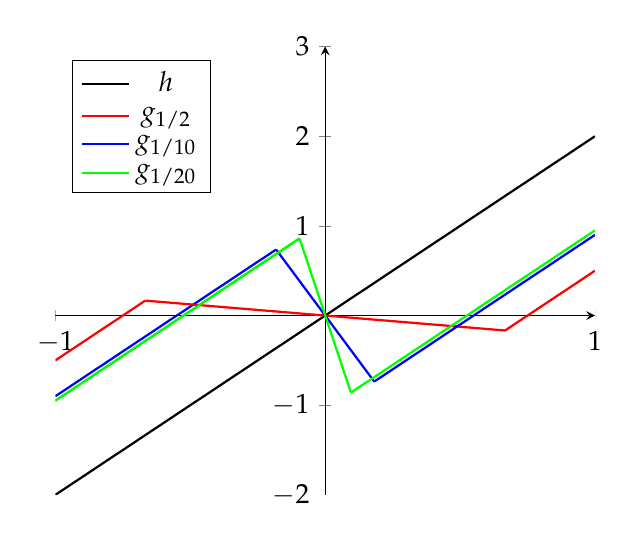
\begin{tikzpicture}\begin{axis}[axis lines = middle, 
xmin=-1,xmax=1,
ymin=-2,ymax=3,     
xtick={-1,0,1},     
ytick={-2,-1,1,2,3},
legend pos= north west,]


\addplot [domain=-1:1,samples=100,color=black,thick] ({x}, {2*x});
\addplot [domain=-1:-0.666,samples=100,color=red,thick] ({x}, {2*x+1+0.5});
\addplot [domain=-1:-0.1818,samples=100,color=blue,thick] ({x}, {2*x+1+0.1});
\addplot [domain=-1:-0.095,samples=100,color=green,thick] ({x}, {2*x+1+0.05});
\addplot [domain=-0.666:0.666,samples=100,color=red,thick] ({x}, {-0.25*x});
\addplot [domain=0.666:1,samples=100,color=red,thick] ({x}, {2*x+1-2.5});
\addplot [domain=-0.1818:0.1818,samples=100,color=blue,thick] ({x}, {-4.05*x});
\addplot [domain=0.1818:1,samples=100,color=blue,thick] ({x}, {2*x+1-2.1});
\addplot [domain=-1:-0.095,samples=100,color=green,thick] ({x}, {2*x+1+0.05});
\addplot [domain=-0.095:0.095,samples=100,color=green,thick] ({x}, {-9.025*x});
\addplot [domain=0.095:1,samples=100,color=green,thick] ({x}, {2*x+1-2.05});


\addlegendentry{$ h $} 
\addlegendentry{$ g_{1/2}$}
\addlegendentry{$ g_{1/10}$} 
\addlegendentry{$ g_{1/20}$}

\end{axis}\end{tikzpicture}\end{center}

Now observe that
\begin{align*}
\int_{-1}^{0}g_{t}(x)\mathrm{d}x & =\int_{-1}^{\frac{-2t}{1+t}}(2x+1+t)\mathrm{d}x+\int_{\frac{-2t}{1+t}}^{0}-\frac{(t-1)^{2}}{2t}x\mathrm{d}x\\
 & =(x^{2}+x+tx)|_{-1}^{\frac{-2t}{1+t}}+\left(\frac{-(t-1)^{2}}{4t}x^{2}\right)|_{\frac{-2t}{1+t}}^{0}\\
 & =\left(\frac{2t}{1+t}\right)^{2}+\left(\frac{-2t}{1+t}\right)+t\left(\frac{-2t}{1+t}\right)-\left(1-1-t\right)+\frac{(t-1)^{2}}{4t}\left(\frac{2t}{1+t}\right)^{2}\\
 & =\left(\frac{(t-1)^{2}}{4t}+1\right)\left(\frac{2t}{1+t}\right)^{2}+(1+t)\left(\frac{-2t}{1+t}\right)+t\\
 & =\frac{(t+1)^{2}}{4t}\frac{4t^{2}}{(1+t)^{2}}-t\\
 & =t-t\\
 & =0.
\end{align*}
Therefore $g_{t}\in\mathcal{Y}$ for all $t\in(0,1]$. Moreover, by
construction we have 
\[
\|g_{t}-h\|_{\infty}=1+t
\]
for all $t\in(0,1]$. This implies $d(h,\mathcal{Y})\leq1$. 

\hfill

\textbf{Step 2: }We claim that there does not exist a $g\in\mathcal{Y}$
such that $\|g-h\|_{\infty}=1$. Indeed, assume for a contradiction
there does exist a $g\in\mathcal{Y}$ such that $\|g-h\|_{\infty}=1$.
Choose such a $g\in\mathcal{Y}$. We may assume that $g$ is real-valued:
if $g$ is not real-valued, then we pass to its real-valued part $u$
and as argued above we obtain $u\in\mathcal{Y}$ and 
\begin{align*}
1 & =\|g-h\|_{\infty}\\
 & =\|u-h\|_{\infty}\\
 & \geq1.
\end{align*}

Since $g$ is real-valued and $\|g-h\|_{\infty}=1$, we have
\[
2x-1\leq g(x)\leq2x+1
\]
for all $x\in[-1,1]$. Since $g$ is continous, we cannot have 
\[
g(x)=\begin{cases}
2x+1 & \text{for all }x\in(-1,0)\\
2x-1 & \text{for all }x\in(0,1).
\end{cases}
\]
Assume $g(x)\neq2x-1$ on the interval $(0,1)$. Choose $c\in(0,1)$
such that $g(c)\neq2c-1$. Since $g$ is continuous and since $g(c)>2c-1$,
there exists $\varepsilon>0$ and $\delta>0$ such that 
\[
g(x)>2x-1+\varepsilon
\]
for all $x\in(c-\delta,c+\delta)$. Choose such $\varepsilon$ and
$\delta$ so that $(c-\delta,c+\delta)\subset(0,1)$. Then
\begin{align*}
0 & =\int_{0}^{1}g(x)\mathrm{d}x\\
 & =\int_{0}^{1}g(x)\mathrm{d}x+\int_{c-\delta}^{c+\delta}g(x)\mathrm{d}x+\int_{c+\delta}^{1}g(x)\mathrm{d}x\\
 & >\int_{0}^{c-\delta}(2x-1)\mathrm{d}x+\int_{c-\delta}^{c+\delta}(2x-1+\varepsilon)\mathrm{d}x+\int_{c+\delta}^{1}(2x-1)\mathrm{d}x\\
 & =\int_{0}^{1}(2x-1)\mathrm{d}x+\int_{c-\delta}^{c+\delta}\varepsilon\mathrm{d}x\\
 & =(x^{2}-x)|_{0}^{1}+\varepsilon x|_{c-\delta}^{c+\delta}\\
 & =2\varepsilon\delta\\
 & >0
\end{align*}
gives us a contradiction.

~~~Thus $g(x)\neq2x+1$ on the interval $(-1,0)$. Choose $c\in(-1,0)$
such that $g(c)\neq2c+1$. Then by a similar argument as above, we
have
\begin{align*}
0 & =\int_{-1}^{0}g(x)\mathrm{d}x\\
 & <\int_{-1}^{0}(2x+1)\mathrm{d}x-\int_{c-\delta}^{c+\delta}\varepsilon\mathrm{d}x\\
 & =-2\varepsilon\delta\\
 & <0,
\end{align*}
which also gives us a contradiction. Therefore there does not exist
a $g\in\mathcal{Y}$ such that $\|g-h\|_{\infty}=1$. \end{proof}

\subsection{Closed Subspaces of $\mathcal{X}^{*}$ and $\mathcal{X}$}

\begin{defn}\label{defn} Let $\mathcal{X}$ be a normed linear space.
For a set $A\subseteq\mathcal{X}$ we define $A^{\perp}$ to be the
subset of $\mathcal{X}^{*}$ consisting of all $\ell\in\mathcal{X}^{*}$
such that $\ell(a)=0$ for all $a\in A$. Similarly, for a set $M\subseteq\mathcal{X}^{*}$
we define $M_{\perp}$ to be the subset of $\mathcal{X}$ consisting
of all vectors $x\in\mathcal{X}$ such that $\ell(x)=0$ for all $\ell\in M$.
\end{defn}

\begin{prop}\label{propclosedsubspacesperpantiperp} Let $\mathcal{X}$
be a normed linear space, let $A$ be a subset of $\mathcal{X}$,
and let $M$ be a subset of $\mathcal{X}^{*}$. Then $A^{\perp}$
and $M_{\perp}$ are closed subspaces of $\mathcal{X}^{*}$ and $\mathcal{X}$
respectively. \end{prop}

\begin{proof} Let $x\in\mathcal{X}$. Define $\widehat{x}\colon\mathcal{X}^{*}\to\mathbb{C}$
by
\[
\widehat{x}(\ell)=\ell(x)
\]
for all $\ell\in\mathcal{X}^{*}$. We claim that $\widehat{x}$ is
a bounded linear functional. To see that $\widehat{x}$ is linear,
let $\ell,\ell'\in\mathcal{X}^{*}$ and let $\lambda,\lambda'\in\mathbb{C}$.
Then
\begin{align*}
\widehat{x}(\lambda\ell+\lambda'\ell') & =(\lambda\ell+\lambda'\ell')(x)\\
 & =\lambda\ell(x)+\lambda'\ell'(x)\\
 & =\lambda\widehat{x}(\ell)+\lambda'\widehat{x}(\ell').
\end{align*}
To see that $\widehat{x}$ is bounded, let $\ell\in\mathcal{X}^{*}$.
Then
\begin{align*}
|\widehat{x}(\ell)| & =|\ell(x)|\\
 & \leq\|x\|\|\ell\|.
\end{align*}
Therefore $\widehat{x}$ is a bounded linear functional. In particular
$\text{ker}\widehat{x}$ is a closed subspace. Thus
\[
A^{\perp}=\bigcap_{a\in A}\text{ker}\widehat{a}\quad\text{and}\quad M_{\perp}=\bigcap_{\ell\in M}\text{ker}\ell
\]
are closed subspaces since an arbitrary intersection of closed subspaces
is a closed subspace. \end{proof}

\begin{prop}\label{prop} Let $\mathcal{X}$ be a normed linear space,
let $A$ be a subset of $\mathcal{X}$, and let $M$ be a subset of
$\mathcal{X}^{*}$. Then $\overline{\text{span}}(A)\subseteq(A^{\perp})_{\perp}$
and $\overline{\text{span}}(M)\subseteq(M_{\perp})^{\perp}$. \end{prop}

\begin{proof} Proposition~(\ref{propclosedsubspacesperpantiperp})
implies $(A^{\perp})_{\perp}$ and $(M_{\perp})^{\perp}$ are closed
subspace. Thus, it suffices to show
\[
\text{span}(A)\subseteq(A^{\perp})_{\perp}\quad\text{and}\quad\text{span}(M)\subseteq(M_{\perp})^{\perp}.
\]
~~~First we show the former. Let $\lambda_{1}a_{1}+\cdots+\lambda_{n}a_{n}\in\text{span}(A)$
and let $\ell\in A^{\perp}$. Then since $\ell(a)=0$ for all $a\in A$,
we have
\begin{align*}
\ell(\lambda_{1}a_{1}+\cdots+\lambda_{n}a_{n}) & =\lambda_{1}\ell(a_{1})+\cdots+\lambda_{n}\ell(a_{n})\\
 & =\lambda_{1}\cdot0+\cdots+\lambda_{n}\cdot0\\
 & =0.
\end{align*}
Since $\ell$ was arbitrary, this implies $\lambda_{1}a_{1}+\cdots+\lambda_{n}a_{n}\in(A^{\perp})_{\perp}$,
and hence $\text{span}(A)\subseteq(A^{\perp})_{\perp}$. 

~~~Now we show the latter. Let $\lambda_{1}\ell_{1}+\cdots+\lambda_{n}\ell_{n}\in\text{span}(M)$
and let $x\in M_{\perp}$. Then since $\ell(x)=0$ for all $\ell\in M$,
we have
\begin{align*}
(\lambda_{1}\ell_{1}+\cdots+\lambda_{n}\ell_{n})(x) & =\lambda_{1}\ell_{1}(x)+\cdots+\lambda_{n}\ell_{n}(x)\\
 & =\lambda_{1}\cdot0+\cdots+\lambda_{n}\cdot0\\
 & =0.
\end{align*}
Since $x$ was arbitrary, this implies $\lambda_{1}\ell_{1}+\cdots+\lambda_{n}\ell_{n}\in(M_{\perp})^{\perp}$,
and hence $\text{span}(M)\subseteq(M_{\perp})^{\perp}$. \end{proof}

\subsection{$(\ell^{1})^{*}$ is isometrically isomorphic to $\ell^{\infty}$.}

\begin{prop}\label{prop} $(\ell^{1})^{*}$ is isometrically isomorphic
to $\ell^{\infty}$. \end{prop}

\begin{proof} For each $n\in\mathbb{N}$, let $e^{n}$ denote the
sequence with entry $1$ in the $n$th component and entry $0$ everywhere
else. Define $\Phi\colon(\ell^{1})^{*}\to\ell^{\infty}$ by
\[
\Phi(\psi)=(\psi(e^{n}))
\]
for all $\psi\in(\ell^{1})^{*}$. Note that for any $\psi\in(\ell^{1})^{*}$,
we have $|(\psi(e^{n}))|\leq\|\psi\|$, and therefore $(\psi(e^{n}))\in\ell^{\infty}$.
We claim that $\|\psi\|=\|\Phi(\psi)\|_{\infty}$. Indeed,
\begin{align*}
\|\Phi(\psi)\|_{\infty} & =\sup\{|\psi(e^{n})|\mid n\in\mathbb{N}\}\\
 & \leq\sup\left\{ \left|\psi\left(\sum_{n=1}^{\infty}a_{n}e^{n}\right)\right|\mid\sum_{n=1}^{\infty}|a_{n}|\leq1\right\} \\
 & =\|\psi\|.
\end{align*}
To prove the reverse inequality assume for a contradiction that $\|\psi\|>\|\Phi(\psi)\|_{\infty}$.
Choose $\varepsilon>0$ and $\sum_{n=1}^{\infty}a_{n}e^{n}\in\ell^{1}$
such that $\sum_{n=1}^{\infty}|a_{n}|\leq1$ and
\begin{equation}
\left|\psi\left(\sum_{n=1}^{\infty}a_{n}e^{n}\right)\right|>\|\Phi(\psi)\|_{\infty}+\varepsilon.\label{eq:strictineq1}
\end{equation}
Choose $N\in\mathbb{N}$ such that $\sum_{n=N}^{\infty}|a_{n}|<\varepsilon/\|\psi\|$
(we can find such an $N$ since $\sum_{n=1}^{\infty}|a_{n}|<\infty$).
Then
\begin{align*}
\left|\psi\left(\sum_{n=1}^{\infty}a_{n}e^{n}\right)\right| & =\left|\psi\left(\sum_{n=1}^{N}a_{n}e^{n}+\sum_{n=N+1}^{\infty}a_{n}e^{n}\right)\right|\\
 & =\left|\psi\left(\sum_{n=1}^{N}a_{n}e^{n}\right)+\psi\left(\sum_{n=N+1}^{\infty}a_{n}e^{n}\right)\right|\\
 & =\left|\sum_{n=1}^{N}a_{n}\psi(e^{n})+\psi\left(\sum_{n=N+1}^{\infty}a_{n}e^{n}\right)\right|\\
 & \leq\left|\sum_{n=1}^{N}a_{n}\psi(e^{n})\right|+\left|\psi\left(\sum_{n=N+1}^{\infty}a_{n}e^{n}\right)\right|\\
 & \leq\sum_{n=1}^{N}|a_{n}||\psi(e^{n})|+\|\psi\|\sum_{n=N+1}^{\infty}|a_{n}|\\
 & <\|\Phi(\psi)\|_{\infty}\sum_{n=1}^{N}|a_{n}|+\|\psi\|\cdot\frac{\varepsilon}{\|\psi\|}\\
 & \leq\|\Phi(\psi)\|_{\infty}+\varepsilon.
\end{align*}
This contradicts (\ref{eq:strictneq1}).

~~~Next we show $\Phi$ is linear. Let $\varphi,\psi\in(\ell^{1})^{*}$
and let $\lambda,\mu\in\mathbb{C}$. Then
\begin{align*}
\Phi(\lambda\varphi+\mu\psi) & =((\lambda\varphi+\mu\psi)(e^{n}))\\
 & =\lambda(\varphi(e^{n}))+\mu(\psi(e^{n}))\\
 & =\lambda\Phi(\varphi)+\mu\Phi(\psi).
\end{align*}

Therefore $\Phi$ is an isometric embedding. 

~~~Now show that $\Phi$ is surjective, and hence an isometric
isomorphism. Let $(a_{n})\in\ell^{\infty}$, let $M=\sup\{|a_{n}|\}$,
and let $E=\text{span}\{e^{n}\mid n\in\mathbb{N}\}$. Define $\varphi\colon E\to\mathbb{C}$
to be the unique linear map such that
\[
\varphi(e^{n})=a_{n}
\]
 for all $n\in\mathbb{N}$. Let $x=x_{n_{1}}e^{n_{1}}+\cdots+x_{n_{k}}e^{n_{k}}\in E$
such that $|x_{n_{1}}|+\cdots+|x_{n_{k}}|\leq1$. Then
\begin{align*}
|\varphi(x_{n_{1}}e^{n_{1}}+\cdots+x_{n_{k}}e^{n_{k}})| & =|x_{n_{1}}\varphi(e^{n_{1}})+\cdots+x_{n_{k}}\varphi(e^{n_{k}})|\\
 & =|x_{n_{1}}a_{n_{1}}+\cdots+x_{n_{k}}a_{n_{k}}|\\
 & \leq|x_{n_{1}}||a_{n_{1}}|+\cdots+|x_{n_{k}}||a_{n_{k}}|\\
 & \leq|x_{n_{1}}|M+\cdots+|x_{n_{k}}||M\\
 & =(|x_{n_{1}}|+\cdots+|x_{n_{k}}||)M\\
 & \leq M
\end{align*}
It follows that $\varphi$ is bounded. By the Hahn-Banach Theorem,
there exists a bounded linear functional $\widetilde{\varphi}$ defined
on all of $\ell^{1}$ such that $\widetilde{\varphi}|_{E}=\varphi$
and $\|\widetilde{\varphi}\|=\|\varphi\|$. Choose such a $\widetilde{\varphi}\in(\ell^{1})^{*}$.
Then clearly $\Phi(\widetilde{\varphi})=(a_{n})$. Therefore $\Phi$
is surjective, and hence an isometric isomorphism. \end{proof}

\section*{Appendix}

\subsection*{Problem 1}

\begin{prop}\label{propsuplinearpositive} Let $A$ be a non-emtpy
set of real numbers which is bounded above and let $\lambda$ be any
non-negative real number. Then
\begin{equation}
\sup(\lambda A)=\lambda\sup(A).\label{eq:sup}
\end{equation}

\end{prop}

\begin{proof} If $\lambda=0$, then (\ref{eq:sup}) is obvious, so
assume $\lambda>0$. Let $\alpha$ denote $\sup(A)$. Choose any element
in $\lambda A$, say $\lambda a$ where $a\in A$. Then since $a\leq\alpha$
and $\lambda$ is non-negative, we have $\lambda a\leq\lambda\alpha$.
This implies
\[
\sup(\lambda A)\leq\lambda\sup(A).
\]
For the reverse direction, observe that
\begin{align*}
\sup(A) & =\sup(\lambda^{-1}\lambda A)\\
 & \leq\lambda^{-1}\sup(\lambda A),
\end{align*}
and this implies 
\[
\sup(\lambda A)\geq\lambda\sup(A).
\]

\end{proof}

\begin{prop}\label{propsuplinearpositive2} Let $A$ and $B$ be non-empty
sets of non-negative real numbers both of which are bounded above.
Then
\begin{equation}
\sup(A+B)=\sup(A)+\sup(B).\label{eq:sup-1}
\end{equation}

\end{prop}

\begin{proof} Let $\alpha$ denote $\sup(A)$, let $\beta$ denote
$\sup(B)$, and let $a+b$ be an arbitrary element in $A+B$. Then
$a\leq\alpha$ and $b\leq\beta$ implies $a+b\leq\alpha+\beta$. Therefore
\begin{equation}
\sup(A+B)\leq\sup(A)+\sup(B).\label{eq:ineqsupadd}
\end{equation}
To show the reverse inequality, we assume (for a contradiction) that
the inequality (\ref{eq:ineqsupadd}) is strict
\[
\sup(A+B)<\sup(A)+\sup(B).
\]
Choose $\varepsilon>0$ such that 
\begin{equation}
\sup(A+B)<\sup(A)+\sup(B)-\varepsilon.\label{supstrictin}
\end{equation}
Choose $a\in A$ and $b\in B$ such that $a>\alpha-\varepsilon/2$
and $b>\beta-\varepsilon/2$. Then
\begin{align*}
a+b & >\alpha-\frac{\varepsilon}{2}+\beta-\frac{\varepsilon}{2}\\
 & =\alpha+\beta-\varepsilon.
\end{align*}
But this contradicts (\ref{supstrictin}). Therefore 
\[
\sup(A+B)\geq\sup(A)+\sup(B).
\]

\end{proof}

\part{Appendix}

\section{Completion}

Let $\mathcal{V}$ be an inner-product space. In this section, we
describe a procedure called \textbf{completion }which constructs a
Hibert space $\mathscr{C}_{\mathcal{V}}\slash\mathscr{C}_{\mathcal{V}}^{0}$
and an injective linear map $\iota\colon\mathcal{V}\to\mathscr{C}_{\mathcal{V}}\slash\mathscr{C}_{\mathcal{V}}^{0}$
such that $\iota$ respects then inner-product structure on both $\mathcal{V}$
and $\mathscr{C}_{\mathcal{V}}\slash\mathscr{C}_{\mathcal{V}}^{0}$
(namely we will show that $\iota$ is an isometry) and such that $\iota(\mathcal{V})$
is dense in $\mathscr{C}_{\mathcal{V}}\slash\mathscr{C}_{\mathcal{V}}^{0}$.

\subsection{Constructing Completions}

Let $\mathscr{C}_{\mathcal{V}}$ denote the set of all Cauchy sequences
in $\mathcal{V}$. We can give $\mathscr{C}_{\mathcal{V}}$ the structure
of a $\mathbb{C}$-vector space as follows: let $(x_{n}),(y_{n})\in\mathscr{C}_{\mathcal{V}}$
and let $\lambda,\mu\in\mathbb{C}$. Then we define
\begin{align}
a(x_{n})+b(y_{n}) & :=(ax_{n}+by_{n}).\label{eq:vectorspacecompletion}
\end{align}
Scalar multiplication and addition as in (\ref{eq:vectorspacecompletion})
are easily seen to give $\mathscr{C}_{\mathcal{V}}$ the structure
of a $\mathbb{C}$-vector space. 

\subsubsection{Pseudo Inner-Product}

A natural contender for an inner-product on $\mathscr{C}_{\mathcal{V}}$
is the map $\langle\cdot,\cdot\rangle\colon\mathscr{C}_{\mathcal{V}}\times\mathscr{C}_{\mathcal{V}}\to\mathbb{C}$
defined by 
\begin{equation}
\langle(x_{n}),(y_{n})\rangle:=\lim_{n\to\infty}\langle x_{n},y_{n}\rangle\label{eq:innerproductcompletion}
\end{equation}
for all $(x_{n}),(y_{n})\in\mathscr{C}_{\mathcal{V}}$. In fact, (\ref{eq:innerproductcompletion})
will not be an inner-product, but rather a \emph{pseudo }inner-product.
Before we explain this however, let us first show that the righthand
side of (\ref{eq:innerproductcompletion}) converges in $\mathbb{C}$

\begin{lemma}\label{lemmacauchybound} Let $(x_{n})$ be a Cauchy
sequence in $\mathcal{V}$. Then $(x_{n})$ is bounded. \end{lemma}

\begin{proof} Let $\varepsilon>0$. Choose $N\in\mathbb{N}$ such
that $n,m\geq N$ implies $\|x_{n}-x_{m}\|<\varepsilon$. Thus, fixing
$m\in\mathbb{N}$, we see that $n\geq N$ implies 
\[
\|x_{n}\|<\|x_{m}\|+\varepsilon.
\]
Now we let 
\[
M=\max\{\|x_{1}\|,\|x_{2}\|,\dots,\|x_{m}\|+\varepsilon\}.
\]
Then $M$ is a bound for $(x_{n})$. \end{proof}

\begin{prop}\label{prop} Let $(x_{n})$ and $(y_{n})$ be Cauchy
sequences of vectors in $\mathcal{V}$. Then $(\langle x_{n},y_{n}\rangle)$
is a Cauchy sequence of complex numbers in $\mathbb{C}$. In particular,
(\ref{eq:innerproductcompletion}) converges in $\mathbb{C}$. \end{prop}

\begin{proof} Let $\varepsilon>0$. Choose $M_{x}$ and $M_{y}$
such that $\|x_{n}\|<M_{x}$ and $\|y_{n}\|<M_{y}$ for all $n\in\mathbb{N}$.
We can do this by Lemma~(\ref{lemmacauchybound}). Next, choose $N\in\mathbb{N}$
such that $n,m\geq N$ implies $\|x_{n}-x_{m}\|<\frac{\varepsilon}{2M_{y}}$
and $\|y_{n}-y_{m}\|<\frac{\varepsilon}{2M_{x}}$. Then $n,m\geq M$
implies 
\begin{align*}
|\langle x_{n},y_{n}\rangle-\langle x_{m},y_{m}\rangle| & =|\langle x_{n},y_{n}\rangle-\langle x_{m},y_{n}\rangle+\langle x_{m},y_{n}\rangle-\langle x_{m},y_{m}\rangle|\\
 & =|\langle x_{n}-x_{m},y_{n}\rangle+\langle x_{m},y_{n}-y_{m}\rangle|\\
 & \leq|\langle x_{n}-x_{m},y_{n}\rangle|+|\langle x_{m},y_{n}-y_{m}\rangle|\\
 & \leq\|x_{n}-x_{m}\|\|y_{n}\|+\|x_{m}\|\|y_{n}-y_{m}\|\\
 & \leq\|x_{n}-x_{m}\|M_{y}+M_{x}\|y_{n}-y_{m}\|\\
 & <\varepsilon.
\end{align*}
This implies $(\langle x_{n},y_{n}\rangle)$ is a Cauchy sequence
of complex numbers in $\mathbb{C}$. The latter statement in the proposition
follows from the fact that $\mathbb{C}$ is complete. \end{proof}

\subsubsection{Quotienting Out To get an Inner-Product}

As mentioned above, (\ref{eq:innerproductcompletion}) is not an inner-product.
It is what's called a pseudo inner-product:

\begin{defn}\label{defn} Let $V$ be a vector space over $\mathbb{C}$.
A map $\langle\cdot,\cdot\rangle\colon V\times V\to\mathbb{C}$ is
called a \textbf{pseudo inner-product on $V$ }if it satisfies the
following properties:
\begin{enumerate}
\item Linearity in the first argument: $\langle x,z\rangle+\langle y,z\rangle=\langle x+y,z\rangle$
and $\langle\lambda x,y\rangle=\lambda\langle x,y\rangle$ for all
$x,y,z\in V$ and $\lambda\in\mathbb{C}$.
\item Conjugate symmetric: $\langle x,y\rangle=\overline{\langle y,x\rangle}$
for all $x,y\in V$.
\item Pseudo positive definiteness: $\langle x,x\rangle\geq0$ for all nonzero
$x\in V$.
\end{enumerate}
A vector space equipped with a pseudo inner-product is called a \textbf{pseudo}
\textbf{inner-product space}. \end{defn} 

~~~To see why (\ref{eq:innerproductcompletion}) is a pseudo inner-product,
note that linearity in the first argument and conjugate symmetry are
clear. What makes (\ref{eq:innerproductcompletion}) a pseudo inner-product
and not an inner-product is that we have pseudo positive definiteness:
\begin{align*}
\langle(x_{n}),(x_{n})\rangle & =\lim_{n\to\infty}\langle x_{n},x_{n}\rangle\\
 & =\lim_{n\to\infty}\|x_{n}\|^{2}\\
 & \geq0.
\end{align*}
In particular, we may have $\langle(x_{n}),(x_{n})\rangle=0$ with
$(x_{n})\neq0$. To remedy this situation, we define
\[
\mathscr{C}_{\mathcal{V}}^{0}:=\left\{ (x_{n})\in\mathscr{C}_{\mathcal{V}}\mid x_{n}\to0\right\} .
\]
Then $\mathscr{C}_{\mathcal{V}}^{0}$ is a subspace of $\mathscr{C}_{\mathcal{V}}$
(if $\lambda\in\mathbb{C}$ and $(x_{n}),(y_{n})\in\mathscr{C}_{\mathcal{V}}^{0}$,
then $(\lambda x_{n}+y_{n})\to0$ and hence $(\lambda x_{n}+y_{n})\in\mathscr{C}_{\mathcal{V}}^{0}$).
Therefore we obtain a quotient space $\mathscr{C}_{\mathcal{V}}\slash\mathscr{C}_{\mathcal{V}}^{0}$.
Now we claim that the pseudo inner-product (\ref{eq:innerproductcompletion})\textbf{
}induces a genuine inner-product, which we denote again by $\langle\cdot,\cdot\rangle$,
on $\mathscr{C}_{\mathcal{V}}\slash\mathscr{C}_{\mathcal{V}}^{0}$,
defined by
\begin{equation}
\langle\overline{(x_{n})},\overline{(y_{n})}\rangle:=\lim_{n\to\infty}\langle x_{n},y_{n}\rangle.\label{eq:innerprodcomp}
\end{equation}
for all $\overline{(x_{n})}$\footnote{When we write \emph{$\overline{(x_{n})}$ }for a coset in $\mathscr{C}_{\mathcal{V}}\slash\mathscr{C}_{\mathcal{V}}^{0}$,
then it is implicitly understood that $(x_{n})$ is an element $\mathscr{C}_{\mathcal{V}}$
which represents the coset \emph{$\overline{(x_{n})}$ }in $\mathscr{C}_{\mathcal{V}}\slash\mathscr{C}_{\mathcal{V}}^{0}$.} and $\overline{(y_{n})}$ in $\mathscr{C}_{\mathcal{V}}\slash\mathscr{C}_{\mathcal{V}}^{0}$.
We need to be sure that (\ref{eq:innerprodcomp}) is well-defined.
Let $(x_{n}')$ and $(y_{n}')$ be different representatives of the
cosets $\overline{(x_{n})}$ and $\overline{(y_{n})}$ respectively
(so $x_{n}-x_{n}'\to0$ and $y_{n}-y_{n}'\to0$). Then
\begin{align*}
\langle\overline{(x_{n}')},\overline{(y_{n}')}\rangle & =\lim_{n\to\infty}\langle x_{n}',y_{n}'\rangle\\
 & =\lim_{n\to\infty}\langle x_{n}',y_{n}'\rangle+\lim_{n\to\infty}\langle x_{n}-x_{n}',y_{n}'\rangle+\lim_{n\to\infty}\langle x_{n},y_{n}-y_{n}'\rangle\\
 & =\lim_{n\to\infty}(\langle x_{n}',y_{n}'\rangle+\langle x_{n}-x_{n}',y_{n}'\rangle+\langle x_{n},y_{n}-y_{n}'\rangle)\\
 & =\lim_{n\to\infty}(\langle x_{n},y_{n}'\rangle+\langle x_{n},y_{n}-y_{n}'\rangle)\\
 & =\lim_{n\to\infty}\langle x_{n},y_{n}\rangle\\
 & =\langle\overline{(x_{n})},\overline{(y_{n})}\rangle.
\end{align*}
Thus (\ref{eq:innerprodcomp}) is well-defined (meaning it is independent
of the choice of representatives of cosets).

~~~Now linearity in the first argument of (\ref{eq:innerprodcomp})
and conjugate symmetry of (\ref{eq:innerprodcomp}) are clear. This
time however, we have positive definiteness: if $\overline{(x_{n})}\in\mathscr{C}_{\mathcal{V}}\slash\mathscr{C}_{\mathcal{V}}^{0}$
such that $\langle\overline{(x_{n})},\overline{(x_{n})}\rangle=0$,
then 
\begin{align*}
\lim_{n\to\infty}\langle x_{n},x_{n}\rangle & =\langle\overline{(x_{n})},\overline{(x_{n})}\rangle\\
 & =0
\end{align*}
implies $x_{n}\to0$, which implies $\overline{(x_{n})}=0$ in $\mathscr{C}_{\mathcal{V}}\slash\mathscr{C}_{\mathcal{V}}^{0}$.

\subsubsection{The map $\iota\colon\mathcal{V}\to\mathscr{C}_{\mathcal{V}}\slash\mathscr{C}_{\mathcal{V}}^{0}$}

Let $\iota\colon\mathcal{V}\to\mathscr{C}_{\mathcal{V}}\slash\mathscr{C}_{\mathcal{V}}^{0}$
be defined by 
\[
\iota(x)=\overline{(x)}_{n\in\mathbb{N}}
\]
for all $x\in\mathcal{V}$, where $(x)_{n\in\mathbb{N}}$ is a constant
sequence in $\mathscr{C}_{\mathcal{V}}$.

\begin{defn}\label{defn} An \textbf{isometry} between inner-product
spaces $\mathcal{V}_{1}$ and $\mathcal{V}_{2}$ is an operator $T\colon\mathcal{V}_{1}\to\mathcal{V}_{2}$
such that
\[
\langle Tx,Ty\rangle=\langle x,y\rangle
\]
for all $x,y\in\mathcal{V}_{1}$. \end{defn}

\begin{rem}\label{rem} Note that an isometry is automatically injective.
Indeed, let $x\in\text{Ker}(T)$. Then 
\begin{align*}
\langle x,y\rangle & =\langle Tx,Ty\rangle\\
 & =\langle0,Ty\rangle\\
 & =0
\end{align*}
for all $y\in\mathcal{V}_{1}$. It follows that $x=0$. \end{rem}

\begin{prop}\label{prop} The map $\iota\colon\mathcal{V}\to\mathscr{C}_{\mathcal{V}}\slash\mathscr{C}_{\mathcal{V}}^{0}$
is an isometry. \end{prop}

\begin{proof}\label{proof} Linearity of $\iota$ is clear. Let $x,y\in\mathcal{V}$.
Then 
\begin{align*}
\langle\langle\iota(x),\iota(y)\rangle & :=\lim_{n\to\infty}\langle x,y\rangle\\
 & =\langle x,y\rangle.
\end{align*}
Thus $\iota$ is an isometry. \end{proof}

\begin{prop}\label{prop} The image of $\mathcal{V}$ under $\iota$
is dense in $\mathscr{C}_{\mathcal{V}}\slash\mathscr{C}_{\mathcal{V}}^{0}$.
In other words, the closure of $\iota(\mathcal{V})$ in $\mathscr{C}_{\mathcal{V}}\slash\mathscr{C}_{\mathcal{V}}^{0}$
is all of $\mathscr{C}_{\mathcal{V}}\slash\mathscr{C}_{\mathcal{V}}^{0}$.
\end{prop}

\begin{proof}\label{proof} Let $\overline{(x_{n})}$ be a coset in
$\mathscr{C}_{\mathcal{V}}\slash\mathscr{C}_{\mathcal{V}}^{0}$. To
show that the closure of $\iota(\mathcal{V})$ is is all of $\mathscr{C}_{\mathcal{V}}\slash\mathscr{C}_{\mathcal{V}}^{0}$,
we construct a sequence of cosets in $\iota(\mathcal{V})$ which converges
to $\overline{(x_{n})}$. Let $\varepsilon>0$ and choose $N\in\mathbb{N}$
such that $n,m\geq N$ implies
\[
\|x_{n}-x_{m}\|<\varepsilon/2.
\]
Then $n,m\geq N$ implies
\begin{align*}
\|\iota(x_{m})-\overline{(x_{n})}\| & =\lim_{n\to\infty}\|x_{m}-x_{n}\|\\
 & <\lim_{n\to\infty}\varepsilon\\
 & =\varepsilon.
\end{align*}
Thus, $(\iota(x_{m}))$ is a sequence of cosets in $\iota(\mathcal{V})$
which converges to $\overline{(x_{n})}$. \end{proof}

\subsubsection{$\mathscr{C}_{\mathcal{V}}\slash\mathscr{C}_{\mathcal{V}}^{0}$ is
a Hilbert Space}

\begin{prop}\label{prop} $\mathscr{C}_{\mathcal{V}}\slash\mathscr{C}_{\mathcal{V}}^{0}$
is a Hilbert space. \end{prop}

\begin{proof}\label{proof} Let $(\overline{x}^{n})$ be a Cauchy
sequence of cosets in $\mathscr{C}_{\mathcal{V}}\slash\mathscr{C}_{\mathcal{V}}^{0}$
where
\[
\overline{x}^{n}=\overline{(x_{k}^{n})}_{k\in\mathbb{N}}
\]
for each $n\in\mathbb{N}$. Throughout the remainder of this proof,
let $\varepsilon>0$.

~~~Since each $x^{n}=(x_{k}^{n})_{k\in\mathbb{N}}$ is a Cauchy
sequence of elements in $\mathcal{V}$, there exists a $\pi(n)\in\mathbb{N}$
such that $k,l\geq\pi(n)$ implies
\[
\|x_{k}^{n}-x_{l}^{n}\|<\frac{\varepsilon}{3}.
\]
For each $n\in\mathbb{N}$, choose such $\pi(n)\in\mathbb{N}$ in
such a way so $\pi(n)\geq\pi(m)$ whenever $n\geq m$.

\hfill

\textbf{Step 1: }We show that the sequence $(x_{\pi(n)}^{n})$ of
elements in $\mathcal{V}$ is a Cauchy sequence. Since $(\overline{x}^{n})$
is a Cauchy sequence of cosets in $\mathscr{C}_{\mathcal{V}}\slash\mathscr{C}_{\mathcal{V}}^{0}$,
there exists an $N\in\mathbb{N}$ such that $n,m\geq N$ implies
\begin{equation}
\|(\overline{x}^{n})-(\overline{x}^{m})\|=\lim_{k\to\infty}\|x_{k}^{n}-x_{k}^{m}\|<\frac{\varepsilon}{4}.\label{eq:cauchyin2}
\end{equation}

Choose such an $N\in\mathbb{N}$. It follows from (\ref{eq:cauchyin2})
that for each $n\geq m\geq N$, there exists $\pi(n,m)\geq\pi(n)$
such that
\[
\|x_{k}^{n}-x_{k}^{m}\|<\frac{\varepsilon}{3}
\]
for all $k\geq\pi(n,m)$. Choose such $\pi(n,m)$ for each $n\geq m\geq N$.
Then if $n\geq m\geq N$, we have
\begin{align*}
\|x_{\pi(n)}^{n}-x_{\pi(m)}^{m}\| & =\|x_{\pi(n)}^{n}-x_{\pi(n,m)}^{n}+x_{\pi(n,m)}^{n}-x_{\pi(n,m)}^{m}+x_{\pi(n,m)}^{m}-x_{\pi(m)}^{m}\|\\
 & \leq\|x_{\pi(n)}^{n}-x_{\pi(n,m)}^{n}\|+\|x_{\pi(n,m)}^{n}-x_{\pi(n,m)}^{m}\|+\|x_{\pi(n,m)}^{m}-x_{\pi(m)}^{m}\|\\
 & <\varepsilon/3+\varepsilon/3+\varepsilon/3\\
 & =\varepsilon.
\end{align*}
Therefore $(x_{\pi(n)}^{n})$ is a Cauchy sequence of elements in
$\mathcal{V}$ and hence represents a coset $\overline{(x_{\pi(n)}^{n})}$
in $\mathscr{C}_{\mathcal{V}}\slash\mathscr{C}_{\mathcal{V}}^{0}$.

\hfill

\textbf{Step 2:} Let $x=(x_{\pi(k)}^{k})$\footnote{Note the change in index from $n$ to $k$.}.
We want to show that the sequence $(\overline{x}^{n})$ of cosets
in $\mathscr{C}_{\mathcal{V}}\slash\mathscr{C}_{\mathcal{V}}^{0}$
converges to the coset $\overline{x}$ in $\mathscr{C}_{\mathcal{V}}\slash\mathscr{C}_{\mathcal{V}}^{0}$.
In particular, we need to find an $N\in\mathbb{N}$ such that $n\geq N$
implies
\[
\|\overline{x}^{n}-\overline{x}\|=\lim_{k\to\infty}\|x_{k}^{n}-x_{\pi(k)}^{k}\|<\varepsilon
\]
or in other words, $n\geq N$ implies
\[
\|x_{k}^{n}-x_{\pi(k)}^{k}\|<\varepsilon
\]
for all $k$ sufficiently large.

~~~Since $x$ is a Cauchy sequence of elements in $\mathcal{V}$,
there exists an $M\in\mathbb{N}$ such that $n,k\geq M$ implies
\[
\|x_{\pi(n)}^{n}-x_{\pi(k)}^{k}\|<2\varepsilon/3.
\]

Choose such an $M\in\mathbb{N}$. Then $n\geq M$ implies
\begin{align*}
\|x_{k}^{n}-x_{\pi(k)}^{k}\| & \leq\|x_{k}^{n}-x_{\pi(n)}^{n}\|+\|x_{\pi(n)}^{n}-x_{\pi(k)}^{k}\|\\
 & <\frac{\varepsilon}{3}+\frac{2\varepsilon}{3}\\
 & =\varepsilon.
\end{align*}
for all $k\geq\max\{M,\pi(n)\}$. \end{proof}

\section{Normed Vector Spaces}

\begin{defn}\label{normedvectorspace} Let $V$ be a $\mathbb{C}$-vector
space. A \textbf{norm }on $V$ is a nonnegative-valued scalar function
$\|\cdot\|\colon V\to[0,\infty)$ such that for all $\lambda\in\mathbb{C}$
and $u,v\in V$, we have 
\begin{enumerate}
\item (Subadditivity) $\|u+v\|\leq\|u\|+\|v\|$,
\item (Absolutely Homogeneous) $\|\lambda v\|=|\lambda|\|v\|$,
\item (Positive-Definite) $\|v\|=0$ if and only if $v=0$.
\end{enumerate}
We call the pair $(V,\|\cdot\|)$ a \textbf{normed vector space}.
\end{defn}

\subsection{Bounded Linear Operators and Normed Vector Spaces}

\begin{defn}\label{defn} Let $\mathcal{V}$ and $\mathcal{W}$ be
inner-product spaces. We define
\[
\mathcal{B}(\mathcal{V},\mathcal{W}):=\{T\colon\mathcal{V}\to\mathcal{W}\mid T\text{ is a bounded linear operator}\}.
\]
$\mathcal{B}(\mathcal{V},\mathcal{W})$ has the structure of a $\mathbb{C}$-vector
space, where addition and scalar multiplication are defined by
\[
(T+U)(x)=Tx+Ux\quad\text{and}\quad(\lambda T)(x)=T(\lambda x)
\]
for all $T,U\in\mathcal{B}(\mathcal{V},\mathcal{W})$, $\lambda\in\mathbb{C}$,
and $v\in\mathcal{V}$. \end{defn}

\begin{prop}\label{prop} Let $\mathcal{V}$ and $\mathcal{W}$ be
inner-product spaces. Then $(\mathcal{B}(\mathcal{V},\mathcal{W}),\|\cdot\|)$
is a normed vector space, where $\|\cdot\|$ is the map which sends
a bounded linear operator $T$ to its norm $\|T\|$. \end{prop}

\begin{proof} An easy exercise in linear algebra shows that $\mathcal{B}(\mathcal{V},\mathcal{W})$
has the structure of a $\mathbb{C}$-vector space, where addition
and scalar multiplication are defined by
\[
(T+U)(x)=T(x)+U(x)\quad\text{and}\quad(\lambda T)(x)=T(\lambda x)
\]
for all $T,U\in\mathcal{B}(\mathcal{V},\mathcal{W})$, $\lambda\in\mathbb{C}$,
and $v\in\mathcal{V}$. The details of this are left as an exercise.
We are more interested in the fact that $\mathcal{B}(\mathcal{V},\mathcal{W})$
is a \emph{normed }vector space. We just need to check that $\|\cdot\|$
satisfies the conditions laid out in Definition~(\ref{normedvectorspace}). 

~~~We first check for subadditivity. Let $T,U\in\mathcal{B}(\mathcal{V},\mathcal{W})$.
Then
\begin{align*}
\|(T+U)(x)\| & =\|Tx+Ux\|\\
 & \leq\|Tx\|+\|Ux\|\\
 & \leq\|T\|\|x\|+\|U\|\|x\|\\
 & =(\|T\|+\|U\|)\|x\|
\end{align*}
for all $x\in\mathcal{V}$. In particular, this implies $\|T+U\|\leq\|T\|+\|U\|$.
Thus we have subadditivity. 

~~~Next we check that $\|\cdot\|$ is absolutely homogeneous. Let
$T\in\mathcal{B}(\mathcal{V},\mathcal{W})$ and let $\lambda\in\mathbb{C}$.
Then 
\begin{align*}
\|(\lambda T)(x)\| & =\|T(\lambda x)\|\\
 & =\|\lambda Tx\|\\
 & =|\lambda|\|Tx\|
\end{align*}
for all $x\in\mathcal{V}$. In particular, this implies $\|\lambda T\|=|\lambda|\|T\|$.
Thus $\|\cdot\|$ is absolutely homogeneous. 

~~~Finally we check for positive-definitiness. Let $T\in\mathcal{B}(\mathcal{V},\mathcal{W})$.
Clearly $\|T\|$ is greater than or equal to $0$ since it is the
supremum of terms which are greater than or equal to $0$. Suppose
$\|T\|=0$. Then
\begin{align*}
\|Tx\| & \leq\|T\|\|x\|\\
 & =0\cdot\|x\|\\
 & =0
\end{align*}
for all $x\in\mathcal{V}$. In particular, this implies $Tx=0$ for
all $x\in\mathcal{V}$ (by positive-definiteness of the norm for $\mathcal{W}$).
Therefore $T=0$ since they agree on all $x\in\mathcal{V}$. \end{proof}

\subsection{Normed Vector Spaces Which Satisfy Parallelogram Law are Inner-Product
Spaces}

\begin{prop}\label{prop} Let $(V,\|\cdot\|)$ be a normed vector
space over $\mathbb{C}$ which satisfies the parallelogram law (\ref{eq:parallelogram}).
Then the map $\langle\cdot,\cdot\rangle\colon V\times V\to\mathbb{C}$
defined by
\begin{equation}
\langle x,y\rangle=\frac{1}{4}\left(\|x+y\|^{2}+i\|x+iy\|^{2}-\|x-y\|^{2}-i\|x-iy\|^{2}\right)\label{eq:innerfromnorm}
\end{equation}
for all $x,y\in V$ is an inner-product. Moreover, the norm induced
by this inner-product is precisely $\|\cdot\|$. In other words, we
have
\[
\langle x,x\rangle=\|x\|^{2}
\]
for all $x\in V$. \end{prop}

\begin{proof} The most difficult part of this proof is showing that
(\ref{eq:innerfromnorm}) is linear in the first argument. Before
we do this, let us show that (\ref{eq:innerfromnorm}) is positive-definite
and conjugate-symmetric. 

~~~For positive-definiteness, let $x\in V$. Then
\begin{align*}
\langle x,x\rangle & =\frac{1}{4}\left(\|2x\|^{2}+i\|x+ix\|^{2}-i\|x-ix\|^{2}\right)\\
 & =\frac{1}{4}\left(\|2x\|^{2}+i((|1+i|^{2}-|1-i|^{2})\|x\|^{2})\right)\\
 & =\|x\|^{2}\\
 & \geq0,
\end{align*}
with equality if and only if $x=0$. Note that this also gives us
$\langle x,x\rangle=\|x\|^{2}$ for all $x\in V$.

~~~For conjugate-symmetry, let $x,y\in V$. Then
\begin{align*}
\overline{\langle y,x\rangle} & =\frac{1}{4}\overline{\left(\|y+x\|^{2}+i\|y+ix\|^{2}-\|y-x\|^{2}-i\|y-ix\|^{2}\right)}\\
 & =\frac{1}{4}\left(\|y+x\|^{2}-i\|y+ix\|^{2}-\|y-x\|^{2}+i\|y-ix\|^{2}\right)\\
 & =\frac{1}{4}\left(\|x+y\|^{2}-i\|i(x-iy)\|^{2}-\|x-y\|^{2}+i\|i(x+iy)\|^{2}\right)\\
 & =\frac{1}{4}\left(\|x+y\|^{2}-i\|x-iy\|^{2}-\|x-y\|^{2}+i\|x+iy\|^{2}\right)\\
 & =\frac{1}{4}\left(\|x+y\|^{2}+i\|x+iy\|^{2}-\|x-y\|^{2}-i\|x-iy\|^{2}\right)\\
 & =\langle x,y\rangle
\end{align*}

~~~Now we come to the difficult part, namely showing that (\ref{eq:innerfromnorm})
is linear in the first argument. We do this in several steps:

\hfill

\textbf{Step 1: }We show that (\ref{eq:innerfromnorm}) is additive
in the first argument (i.e. $\langle x+z,y\rangle=\langle x,y\rangle+\langle z,y\rangle$
for all $x,y,z\in V$). Let $x,y,z\in V$. First note that by the
parallelogram law (\ref{eq:parallelogram}), we have
\begin{align*}
\|x+z+y\|^{2}-\|x+z-y\|^{2} & =2\|x+y\|^{2}+2\|z\|^{2}-\|x+y-z\|^{2}-2\|x-y\|^{2}-2\|z\|^{2}+\|x-y-z\|^{2}\\
 & =2\|x+y\|^{2}-2\|x-y\|^{2}-\|z-y-x\|^{2}+\|z+y-x\|^{2}\\
 & =2\|x+y\|^{2}-2\|x-y\|^{2}-2\|z-y\|^{2}-2\|x\|^{2}+\|z-y+x\|^{2}+2\|z+y\|^{2}+2\|x\|^{2}-\|z+y+x\|^{2}\\
 & =2\|x+y\|^{2}-2\|x-y\|^{2}+2\|z+y\|^{2}-2\|z-y\|^{2}+\|x+z-y\|^{2}-\|x+z+y\|^{2}.
\end{align*}
Adding $\|x+z-y\|^{2}-\|x+z+y\|^{2}$ to both sides gives us
\begin{align*}
2(\|x+z+y\|^{2}-\|x+z-y\|^{2}) & =2(\|x+y\|^{2}-\|x-y\|^{2}+\|z+y\|^{2}-\|z-y\|^{2}),
\end{align*}
and after cancelling $2$ from both sides, we obtain
\begin{align*}
\|x+z+y\|^{2}-\|x+z-y\|^{2} & =\|x+y\|^{2}-\|x-y\|^{2}+\|z+y\|^{2}-\|z-y\|^{2}.
\end{align*}
Therefore
\begin{align*}
\langle x+z,y\rangle & =\frac{1}{4}\left(\|x+z+y\|^{2}+i\|x+z+iy\|^{2}-\|x+z-y\|^{2}-i\|x+z-iy\|^{2}\right)\\
 & =\frac{1}{4}\left(\|x+z+y\|^{2}-\|x+z-y\|^{2}+i(\|x+z+iy\|^{2}-\|x+z-iy\|^{2})\right)\\
 & =\frac{1}{4}\left(\|x+y\|^{2}-\|x-y\|^{2}+\|z+y\|^{2}-\|z-y\|^{2}+i(\|x+iy\|^{2}-\|x-iy\|^{2}+\|z+iy\|^{2}-\|z-iy\|^{2})\right)\\
 & =\frac{1}{4}\left(\|x+y\|^{2}-\|x-y\|^{2}+\|z+y\|^{2}-\|z-y\|^{2}+i(\|x+iy\|^{2}-\|x-iy\|^{2}+\|z+iy\|^{2}-\|z-iy\|^{2})\right)\\
 & =\frac{1}{4}\left(\|x+y\|^{2}+i\|x+iy\|^{2}-\|x-y\|^{2}-i\|x-iy\|^{2}+\|z+y\|^{2}+i\|z+iy\|^{2}-\|z-y\|^{2}-i\|z-iy\|^{2}\right)\\
 & =\langle x,y\rangle+\langle z,y\rangle.
\end{align*}
Thus we have additivity in the first argument.

\hfill

\textbf{Step 2: }We show that (\ref{eq:innerfromnorm}) respects $\mathbb{Q}$-scaling
in the first argument (i.e. $\frac{m}{n}\langle x,y\rangle=\langle\frac{m}{n}x,y\rangle$
for all rational numbers $\frac{m}{n}\in\mathbb{Q}$ and for all $x,y\in V$.
Let $\frac{m}{n}\in\mathbb{Q}$ and let $x,y\in V$. Then since (\ref{eq:innerfromnorm})
is additive in the first argument and since $V$ is a $\mathbb{C}$-vector
space, we have
\begin{align*}
\frac{m}{n}\langle x,y\rangle & =\frac{m}{n}\left\langle \frac{n}{n}x,y\right\rangle \\
 & =\frac{mn}{n}\left\langle \frac{1}{n}x,y\right\rangle \\
 & =m\left\langle \frac{1}{n}x,y\right\rangle \\
 & =\left\langle \frac{m}{n}x,y\right\rangle .
\end{align*}
Therefore (\ref{eq:innerfromnorm}) respects $\mathbb{Q}$-scaling
in the first argument.

\hfill

\textbf{Step 3: }We show that (\ref{eq:innerfromnorm}) respects $\mathbb{R}$-scaling
in the first argument. First note that $y\in V$, the map $\langle\cdot,y\rangle\colon V\to\mathbb{C}$
is continuous. Let $x,y\in V$ and let $r\in\mathbb{R}$. Choose a
sequence $(r_{n})$ of rational numbers such that $r_{n}\to r$ (we
can do this since $\mathbb{Q}$ is dense in $\mathbb{R}$). Then we
have
\begin{align*}
\langle rx,y\rangle & =\lim_{n\to\infty}\langle r_{n}x,y\rangle\\
 & =\lim_{n\to\infty}r_{n}\langle x,y\rangle\\
 & =r\langle x,y\rangle.
\end{align*}
Therefore (\ref{eq:innerfromnorm}) respects $\mathbb{R}$-scaling
in the first component.

\textbf{Step 4: }We show that (\ref{eq:innerfromnorm}) respects $\mathbb{C}$-scaling
in the first component. We first show that $\langle ix,y\rangle=i\langle x,y\rangle$
for all $x,y\in V$. 

~~~Let $x,y\in V$. Then
\begin{align*}
\langle ix,y\rangle & =\frac{1}{4}\left(\|ix+y\|^{2}+i\|ix+iy\|^{2}-\|ix-y\|^{2}-i\|ix-iy\|^{2}\right)\\
 & =\frac{1}{4}\left(\|x-iy\|^{2}+i\|x+y\|^{2}-\|x+iy\|^{2}-i\|x-y\|^{2}\right)\\
 & =\frac{1}{4}\left(i\|x+y\|^{2}-\|x+iy\|^{2}-i\|x-y\|^{2}+\|x-iy\|^{2}\right)\\
 & =\frac{i}{4}\left(\|x+y\|^{2}+i\|x+iy\|^{2}-\|x-y\|^{2}-i\|x-iy\|^{2}\right)\\
 & =i\langle x,y\rangle.
\end{align*}

Now let $\lambda=r+is\in\mathbb{C}$. Then we have
\begin{align*}
\langle\lambda x,y\rangle & =\langle(r+is)x,y\rangle\\
 & =\langle rx+isx,y\rangle\\
 & =\langle rx,y\rangle+\langle isx,y\rangle\\
 & =r\langle x,y\rangle+s\langle ix,y\rangle\\
 & =r\langle x,y\rangle+is\langle x,y\rangle\\
 & =(r+is)\langle x,y\rangle\\
 & =\lambda\langle x,y\rangle
\end{align*}
for all $x,y\in V$. Therefore (\ref{eq:innerfromnorm}) respects
$\mathbb{C}$-scaling in the first component. \end{proof}

\subsection{Distances and Pseudo Normed Vector Spaces}

Let $\mathcal{V}$ be an inner-product space and let $\mathcal{A}$
be a subspace of $\mathcal{V}$. We define
\begin{equation}
d(x,\mathcal{A})=\inf\{\|x-a\|\mid a\in A\}\label{eq:pseudonorm}
\end{equation}
for all $x\in\mathcal{V}$. The map $d(-,\mathcal{A})$ is a good
candidate for a norm on $\mathcal{V}$. It turns out however that
$d(-,\mathcal{A})$ is just a \textbf{pseudo norm}. 

\begin{defn}\label{defn} Let $V$ be a vector space over $\mathbb{C}$.
A map $p\colon V\to[0,\infty)$ is called a \textbf{pseudo norm on
$V$ }if it satisfies the following properties:
\begin{enumerate}
\item (Subadditivity) $p(u+v)\leq p(u)+p(v)$ for all $u,v\in V$,
\item (Absolutely Homogeneous) $p(\lambda v)=|\lambda|p(v)$ for all $v\in V$
and $\lambda\in\mathbb{C}$.
\end{enumerate}
A vector space equipped with a pseudo inner-product is called a \textbf{pseudo}
\textbf{normed vector space}. \end{defn} 

\begin{rem}\label{rem} Thus a norm is just a pseudo norm with the
positive-definiteness property. \end{rem}

\subsubsection{Absolute Homogeneity of Distances}

\begin{prop}\label{prop} Let $\mathcal{V}$ be an inner-product space,
let $\mathcal{A}$ be a subspace of $\mathcal{V}$, let $x\in\mathcal{V}$,
and let $\lambda\in\mathbb{C}$. Then 
\[
d(\lambda x,\mathcal{A})=|\lambda|d(x,\mathcal{A}).
\]
\end{prop}

\begin{proof} Choose a sequence $(y_{n})$ of elements in $\mathcal{A}$
such that
\[
\|x-y_{n}\|<d(x,\mathcal{A})+\frac{1}{|\lambda n|}
\]
for all $n\in\mathbb{N}$. Then since $\mathcal{A}$ is a subspace,
we have
\begin{align*}
d(\lambda x,\mathcal{A}) & \leq\|\lambda x-\lambda y_{n}\|\\
 & =|\lambda|\|x-y_{n}\|\\
 & <|\lambda|\left(d(x,\mathcal{A})+\frac{1}{|\lambda n|}\right)\\
 & =|\lambda|d(x,\mathcal{A})+\frac{1}{n}
\end{align*}
for all $n\in\mathbb{N}$. In particular, this implies $d(\lambda x,\mathcal{A})\leq|\lambda|d(x,\mathcal{A})$. 

~~~Conversely, choose a sequence $(z_{n})$ of elements in $\mathcal{A}$
such that
\[
\|\lambda x-z_{n}\|<d(\lambda x,\mathcal{A})+\frac{1}{n}
\]

Then since $\mathcal{A}$ is a subspace, we have
\begin{align*}
|\lambda|d(x,\mathcal{A}) & \leq|\lambda|\|x-z_{n}/|\lambda|\|\\
 & =\|\lambda x-z_{n}\|\\
 & <d(\lambda x,\mathcal{A})+\frac{1}{n}
\end{align*}
for all $n\in\mathbb{N}$. In particular, this implies $|\lambda|d(x,\mathcal{A})\leq d(\lambda x,\mathcal{A})$.
\end{proof}

\subsubsection{Subadditivity of Distances}

\begin{prop}\label{prop} Let $\mathcal{V}$ be an inner-product space,
let $\mathcal{A}$ be a subspace of $\mathcal{V}$, and let $x,y\in\mathcal{V}$.
Then 
\[
d(x+y,\mathcal{A})\leq d(x,\mathcal{A})+d(y,\mathcal{A}).
\]
\end{prop}

\begin{proof} Choose a sequences $(w_{n})$ and $(z_{n})$ of elements
in $\mathcal{A}$ such that 
\[
\|x-w_{n}\|<d(x,\mathcal{A})+\frac{1}{2n}\quad\text{and}\quad\|y-z_{n}\|<d(y,\mathcal{A})+\frac{1}{2n}
\]
for all $n\in\mathbb{N}$. Then since $\mathcal{A}$ is a subspace,
we have
\begin{align*}
d(x+y,\mathcal{A}) & \leq\|(x+y)-(w_{n}+z_{n})\|\\
 & \leq\|x-w_{n}\|+\|y-z_{n}\|\\
 & <d(x,\mathcal{A})+\frac{1}{2n}+d(y,\mathcal{A})+\frac{1}{2n}\\
 & =d(x,\mathcal{A})+d(y,\mathcal{A})+\frac{1}{n}
\end{align*}
for all $n\in\mathbb{N}$. In particular, this implies $d(x+y,\mathcal{A})\leq d(x,\mathcal{A})+d(y,\mathcal{A})$.
\end{proof}

\subsubsection{Quotienting out to get a Norm}

To see why (\ref{eq:pseudonorm}) is just a pseudo norm and not a
norm, note that $d(x,\mathcal{A})=0$ if and only if $x\in\overline{\mathcal{A}}$.
To remedy this situation, we quotient out by $\overline{\mathcal{A}}$.
First we need a lemma. 

\begin{lemma}\label{lemma} Let $x\in\mathcal{V}$. Then $d(x,\mathcal{A})=d(x,\overline{\mathcal{A}})$.
\end{lemma}

\begin{proof} We have $d(x,\mathcal{A})\geq d(x,\overline{\mathcal{A}})$
since $\mathcal{A}\subseteq\overline{\mathcal{A}}$. For the reverse
inequality, we assume (for a contradiction) that $d(x,\mathcal{A})>d(x,\overline{\mathcal{A}})$.
For the reverse inequality, let $\varepsilon>0$. Choose $a\in\mathcal{\overline{A}}$
such that
\[
\|x-a\|<d(x,\overline{\mathcal{A}})+\varepsilon/2.
\]
Choose $b\in\mathcal{A}$ such that $\|a-b\|<\varepsilon/2.$ Then
\begin{align*}
d(x,\mathcal{A}) & \leq\|x-b\|\\
 & \leq\|x-a\|+\|a-b\|\\
 & <d(x,\overline{\mathcal{A}})+\varepsilon/2+\varepsilon/2\\
 & =d(x,\overline{\mathcal{A}})+\varepsilon.
\end{align*}
Since this holds for all $\varepsilon>0$, we have $d(x,\mathcal{A})\leq d(x,\overline{\mathcal{A}})$.
\end{proof}

\begin{prop}\label{prop} The pseudo norm $d(-,\mathcal{A})$ on $\mathcal{V}$
induces a well-defined norm $\|\cdot\|$ on $\mathcal{V}\slash\overline{\mathcal{A}}$,
defined by
\begin{equation}
\|\overline{x}\|=d(x,\mathcal{A})\label{normfrom}
\end{equation}
for all $\overline{x}\in\mathcal{V}\slash\overline{\mathcal{A}}$.
\end{prop}

\begin{proof} We first check that (\ref{normfrom}) is well-defined.
Let $\overline{x}\in\mathcal{V}\backslash\overline{\mathcal{A}}$\footnote{Do not confuse the overline over $\mathcal{A}$ with the overline
over $x$. One denotes the closure of $\mathcal{A}$ and the other
denotes a coset in $\mathcal{V}\slash\overline{\mathcal{A}}$ with
a given represenative $x\in\mathcal{V}$. }. Choose another representative of the coset $\overline{x}$, say
$x+a$ where $a\in\overline{\mathcal{A}}$. Then
\begin{align*}
\|\overline{x+a}\| & =d(x+a,\mathcal{A})\\
 & =d(x+a,\overline{\mathcal{A}})\\
 & =\inf\{\|x+a-b\|\mid b\in\overline{\mathcal{A}}\}\\
 & =\inf\{\|x-c\|\mid c\in\overline{\mathcal{A}}\}\\
 & =d(x,\mathcal{A})\\
 & =\|\overline{x}\|.
\end{align*}
Thus $\|\cdot\|$ is well-defined. 

~~~Now $\|\cdot\|$ is a pseudo norm on $\mathcal{V}\backslash\overline{\mathcal{A}}$
since it inherits these properties from $d(-,\mathcal{A})$ on $\mathcal{V}$.
Indeed, for subadditivity, we have
\begin{align*}
\|\overline{x}+\overline{y}\| & =d(x+y,\mathcal{A})\\
 & \leq d(x,\mathcal{A})+d(y,\mathcal{A})\\
 & =\|\overline{x}\|+\|\overline{y}\|
\end{align*}
for all $\overline{x},\overline{y}\in\mathcal{V}\backslash\overline{\mathcal{A}}$,
and for absolute homogeneity, we have
\begin{align*}
\|\lambda\overline{x}\| & =d(\lambda x,\mathcal{A})\\
 & =|\lambda|d(x,\mathcal{A})\\
 & =|\lambda|\|\overline{x}\|
\end{align*}
for all $\overline{x}\in\mathcal{V}\backslash\overline{\mathcal{A}}$
and $\lambda\in\mathbb{C}$. 

~~~Moreover $\|\cdot\|$ is a norm on $\mathcal{V}\backslash\overline{\mathcal{A}}$
since we also have positive-definiteness. Indeed, let $\overline{x}\in\mathcal{V}\slash\overline{\mathcal{A}}$.
Then
\begin{align*}
\overline{x}=0 & \iff x\in\overline{\mathcal{A}}\\
 & \iff d(x,\mathcal{A})=0\\
 & \iff\|\overline{x}\|=0.
\end{align*}

\end{proof}

\section{Duality}

Let $K$ be a field, let $V$ be a $K$-vector space with basis $\beta=\{\beta_{1},\dots,\beta_{m}\}$,
and let $W$ be a $K$-vector space with basis $\gamma=\{\gamma_{1},\dots,\gamma_{n}\}$.
Recall from linear algebra that we define\textbf{ }the \textbf{(algebraic)
dual} of $V$ to be the $K$-vector space
\[
V^{\star}:=\{\varphi\colon V\to K\mid\varphi\text{ is linear}\}.
\]
where addition and scalar multiplication are defined by
\[
(\varphi+\psi)(v)=\varphi(v)+\psi(v)\quad\text{and}\quad(\lambda\varphi)(v)=\varphi(\lambda v)
\]
for all $\varphi,\psi\in V^{\star}$, $\lambda\in\mathbb{C}$, and
$v\in V$. The \textbf{(algebraic) dual }of $\beta$ is defined to
be the basis of $V^{\star}$ given by $\beta^{\star}:=\{\beta_{1}^{\star},\dots,\beta_{m}^{\star}\}$,
where each $\beta_{i}^{\star}$ is uniquely determined by
\[
\beta_{i}^{\star}(\beta_{j})=\begin{cases}
1 & \text{if }i=j\\
0 & \text{else}
\end{cases}
\]
If $T\colon V\to W$ is a linear map, we define its \textbf{(algebraic)
dual }to be the linear map $T^{\star}\colon W^{\star}\to V^{\star}$
defined by
\[
T^{\star}(\varphi)=\varphi\circ T
\]
for all $\varphi\in W^{\star}$. One learns in linear algebra that
the transpose of the matrix representation of $T$ with respect to
the bases $\beta$ and $\gamma$ is equal to the matrix representation
of $T^{\star}$ with respect to the bases $\gamma^{\star}$ and $\beta^{\star}$.
In terms of notation, this is written as
\[
([T]_{\beta}^{\gamma})^{\top}=[T^{\star}]_{\gamma^{\star}}^{\beta^{\star}}.
\]

We want to describe an analog of this situation for inner-product
spaces over $\mathbb{C}$.

\begin{defn}\label{defn} Let $\mathcal{V}$ be an inner-product space
over $\mathbb{C}$. We define its \textbf{(continuous) dual space}\footnote{When speaking about the dual space of an inner-product space, we will
always mean its continuous dual.}\textbf{ }to be
\begin{align*}
\mathcal{V}^{*} & :=\{\ell\colon\mathcal{V}\to\mathbb{C}\mid\ell\text{ is linear and continuous}\}.\\
 & =\{\ell\colon\mathcal{V}\to\mathbb{C}\mid\ell\text{ is a bounded operator}\}.
\end{align*}

\end{defn}

\begin{rem}\label{rem} Thus $\mathcal{V}^{*}$ captures both topological
and linear aspects of $\mathcal{V}$. \end{rem}

\subsection{Riesz Representation Theorem Revisited}

\begin{theorem}\label{theorem} (Riesz Representation Theorem) Let
$\mathcal{H}$ be a Hilbert space. Then there exists an isometric
antiisomorphism $\Phi\colon\mathcal{H}\to\mathcal{H}^{*}$. \end{theorem}

\begin{proof}\label{proof} Define $\Phi\colon\mathcal{H}\to\mathcal{H}^{*}$
by
\[
\Phi(x)=\langle\cdot,x\rangle
\]
for all $x\in\mathcal{H}$. We first show $\Phi$ is antilinear. Let
$x,y\in\mathcal{H}$ and let $\lambda,\mu\in\mathbb{C}$. Then 
\begin{align*}
\Phi(\lambda x+\mu y)(z) & =\langle z,\lambda x+\mu y\rangle\\
 & =\overline{\lambda}\langle z,x\rangle+\overline{\mu}\langle z,y\rangle\\
 & =\overline{\lambda}\Phi(x)(z)+\overline{\mu}\Phi(y)(z)
\end{align*}
for all $z\in\mathcal{H}$. Therefore $\Phi$ is antilinear.

~~~Note $\Phi$ is an injective antilinear map since the inner-product
is positive-definite. Also, the Riesz representation theorem implies
$\Phi$ is surjective. Finally Example~(\ref{exampleriesz}) implies
$\Phi$ is an isometry. Therefore $\Phi$ is an isometric antiisomorphism.
\end{proof}

\section{Limit Infimum}

Let $(a_{n})$ be a sequence of positive real numbers. We define the
\textbf{limit infimum }of $(a_{n})$, denoted $\liminf(a_{n})$, to
be the limit
\begin{equation}
\liminf(a_{n}):=\lim_{N\to\infty}(\inf\{a_{n}\mid n\geq N\}).\label{eq:liminf-1}
\end{equation}

Since the sequence $(\inf\{a_{n}\mid n\geq N\})_{N\in\mathbb{N}}$
is a monotone increasing sequence in $N$, the limit (\ref{eq:liminf-1})
always exists or equals $-\infty$.

\begin{prop}\label{proplimsup} Let $(a_{n})$ be a sequence of positive
real-valued numbers.
\begin{enumerate}
\item If $\liminf(a_{n})=A$, then for each $\varepsilon>0$ and $N\in\mathbb{N}$,
there exists some $n\geq N$ such that $a_{n}>A+\varepsilon$. In
other words, for all $\varepsilon>0$, the sequence $(a_{n})$ is
frequently strictly less than $A+\varepsilon$. 
\item If $\liminf(a_{n})=A$, then for each $\varepsilon>0$, there exists
$N\in N$ such that $a_{n}>A-\varepsilon$ for all $n\geq N$. In
other words, for all $\varepsilon>0$, the sequence $(a_{n})$ is
eventually strictly greater than $A-\varepsilon$. 
\item Conversely, if $A\geq0$ satisfies 1 and 2, then $\text{liminf}(a_{n})=A$.
\end{enumerate}
\end{prop}

\begin{proof}\hfill

\hfill

1. We prove this by contradiction. To obtain a contradiction, assume
that there there exists $\varepsilon>0$ and $N\in\mathbb{N}$ such
that there does not exist any $n\geq N$ with $a_{n}<A+\varepsilon$.
Choose such $\varepsilon>0$ and $N\in\mathbb{N}$. Then $a_{n}\geq A+\varepsilon$
for all $n\geq N$. This implies $\inf\{a_{n}\mid n\geq N\}>A+\varepsilon$.
Since $\inf\{a_{n}\mid n\geq N\}$ is a monotone increasing function
of $N$, this implies $\liminf(a_{n})\geq A+\varepsilon$, which is
a contradiction. 

\hfill

2. We prove this by contradiction. To obtain a contradiction, assume
that there exists $\varepsilon>0$ such that there does not exist
an $N\in\mathbb{N}$ with $a_{n}>A-\varepsilon$ for all $n\geq N$.
Choose such $\varepsilon>0$ and let $N\in\mathbb{N}$. Then there
exists $n\geq N$ such that $a_{n}\leq A-\varepsilon$. In particular,
this implies
\[
\inf\{a_{n}\mid n\geq N\}\leq A-\varepsilon
\]
Since $N$ is arbitrary, this further implies
\begin{align*}
\liminf(a_{n}) & =\lim_{N\to\infty}(\inf\{a_{n}\mid n\geq N\})\\
 & \leq A-\varepsilon,
\end{align*}
which contradicts the fact that $\liminf(a_{n})=A$. 

\hfill

3. Let $A\geq0$ satisfy 1 and 2 and let $A'=\liminf(a_{n})$. We
prove by contradiction that $A=A'$. Assume for a contradiction that
$A<A'$. Let $\varepsilon=A'-A$. Since $A'$ satisfies 2, the sequence
$(a_{n})$ is eventually greater than $A'-\varepsilon/2$. On the
other hand, since $A$ satisfies 1, the sequence $(a_{n})$ is frequently
less than $A+\varepsilon/2=A'-\varepsilon/2$. This is a contradiciton.
An analagous argument gives a contradiction when we assume $A>A'$.
Therefore $A=A'$. \end{proof}

\begin{lemma}\label{lemma} Let $(a_{n})$ and $(b_{n})$ be two sequences
of positive real numbers such that $\liminf(a_{n})=A$ and $\liminf(b_{n})=B$.
Then
\begin{enumerate}
\item $\liminf(a_{n}b_{n})=AB$
\item $\liminf(a_{n}+b_{n})=A+B$
\end{enumerate}
\end{lemma}

\begin{proof}\hfill

\hfill

1. Let $\varepsilon>0$. Since the sequence $(a_{n})$ is eventually
greater than $A-\varepsilon/(A+B)$ and since the sequence $(b_{n})$
is eventually greater than $B-\varepsilon/(A+B)$, the sequence $(a_{n}b_{n})$
is eventually greater than
\begin{align*}
\left(A-\frac{\varepsilon}{A+B}\right)\left(B-\frac{\varepsilon}{A+B}\right) & =AB-\frac{\varepsilon(A+B)}{(A+B)}+\frac{\varepsilon^{2}}{(A+B)^{2}}\\
 & \geq AB-\varepsilon.
\end{align*}

An analagous argument shows that $(a_{n}b_{n})$ is frequently less
than $AB+\varepsilon$. 

\hfill

2. This is proved in the same way as 1. \end{proof}
\end{document}
